\documentclass[twoside]{book}

% Packages required by doxygen
\usepackage{fixltx2e}
\usepackage{calc}
\usepackage{doxygen}
\usepackage[export]{adjustbox} % also loads graphicx
\usepackage{graphicx}
\usepackage[utf8]{inputenc}
\usepackage{makeidx}
\usepackage{multicol}
\usepackage{multirow}
\PassOptionsToPackage{warn}{textcomp}
\usepackage{textcomp}
\usepackage[nointegrals]{wasysym}
\usepackage[table]{xcolor}

% Font selection
\usepackage[T1]{fontenc}
\usepackage[scaled=.90]{helvet}
\usepackage{courier}
\usepackage{amssymb}
\usepackage{sectsty}
\renewcommand{\familydefault}{\sfdefault}
\allsectionsfont{%
  \fontseries{bc}\selectfont%
  \color{darkgray}%
}
\renewcommand{\DoxyLabelFont}{%
  \fontseries{bc}\selectfont%
  \color{darkgray}%
}
\newcommand{\+}{\discretionary{\mbox{\scriptsize$\hookleftarrow$}}{}{}}

% Page & text layout
\usepackage{geometry}
\geometry{%
  a4paper,%
  top=2.5cm,%
  bottom=2.5cm,%
  left=2.5cm,%
  right=2.5cm%
}
\tolerance=750
\hfuzz=15pt
\hbadness=750
\setlength{\emergencystretch}{15pt}
\setlength{\parindent}{0cm}
\setlength{\parskip}{3ex plus 2ex minus 2ex}
\makeatletter
\renewcommand{\paragraph}{%
  \@startsection{paragraph}{4}{0ex}{-1.0ex}{1.0ex}{%
    \normalfont\normalsize\bfseries\SS@parafont%
  }%
}
\renewcommand{\subparagraph}{%
  \@startsection{subparagraph}{5}{0ex}{-1.0ex}{1.0ex}{%
    \normalfont\normalsize\bfseries\SS@subparafont%
  }%
}
\makeatother

% Headers & footers
\usepackage{fancyhdr}
\pagestyle{fancyplain}
\fancyhead[LE]{\fancyplain{}{\bfseries\thepage}}
\fancyhead[CE]{\fancyplain{}{}}
\fancyhead[RE]{\fancyplain{}{\bfseries\leftmark}}
\fancyhead[LO]{\fancyplain{}{\bfseries\rightmark}}
\fancyhead[CO]{\fancyplain{}{}}
\fancyhead[RO]{\fancyplain{}{\bfseries\thepage}}
\fancyfoot[LE]{\fancyplain{}{}}
\fancyfoot[CE]{\fancyplain{}{}}
\fancyfoot[RE]{\fancyplain{}{\bfseries\scriptsize Generated by Doxygen }}
\fancyfoot[LO]{\fancyplain{}{\bfseries\scriptsize Generated by Doxygen }}
\fancyfoot[CO]{\fancyplain{}{}}
\fancyfoot[RO]{\fancyplain{}{}}
\renewcommand{\footrulewidth}{0.4pt}
\renewcommand{\chaptermark}[1]{%
  \markboth{#1}{}%
}
\renewcommand{\sectionmark}[1]{%
  \markright{\thesection\ #1}%
}

% Indices & bibliography
\usepackage{natbib}
\usepackage[titles]{tocloft}
\setcounter{tocdepth}{3}
\setcounter{secnumdepth}{5}
\makeindex

% Hyperlinks (required, but should be loaded last)
\usepackage{ifpdf}
\ifpdf
  \usepackage[pdftex,pagebackref=true]{hyperref}
\else
  \usepackage[ps2pdf,pagebackref=true]{hyperref}
\fi
\hypersetup{%
  colorlinks=true,%
  linkcolor=blue,%
  citecolor=blue,%
  unicode%
}

% Custom commands
\newcommand{\clearemptydoublepage}{%
  \newpage{\pagestyle{empty}\cleardoublepage}%
}

\usepackage{caption}
\captionsetup{labelsep=space,justification=centering,font={bf},singlelinecheck=off,skip=4pt,position=top}

%===== C O N T E N T S =====

\begin{document}

% Titlepage & ToC
\hypersetup{pageanchor=false,
             bookmarksnumbered=true,
             pdfencoding=unicode
            }
\pagenumbering{alph}
\begin{titlepage}
\vspace*{7cm}
\begin{center}%
{\Large Drawing Client \\[1ex]\large 1 }\\
\vspace*{1cm}
{\large Generated by Doxygen 1.8.12}\\
\end{center}
\end{titlepage}
\clearemptydoublepage
\pagenumbering{roman}
\tableofcontents
\clearemptydoublepage
\pagenumbering{arabic}
\hypersetup{pageanchor=true}

%--- Begin generated contents ---
\chapter{Namespace Index}
\section{Namespace List}
Here is a list of all namespaces with brief descriptions\+:\begin{DoxyCompactList}
\item\contentsline{section}{\hyperlink{namespacefunc}{func} }{\pageref{namespacefunc}}{}
\end{DoxyCompactList}

\chapter{Hierarchical Index}
\section{Class Hierarchy}
This inheritance list is sorted roughly, but not completely, alphabetically\+:\begin{DoxyCompactList}
\item \contentsline{section}{Color}{\pageref{class_color}}{}
\item \contentsline{section}{Drawing\+Visitor}{\pageref{class_drawing_visitor}}{}
\begin{DoxyCompactList}
\item \contentsline{section}{Qt\+Drawer}{\pageref{class_qt_drawer}}{}
\item \contentsline{section}{Server\+Drawer}{\pageref{class_server_drawer}}{}
\end{DoxyCompactList}
\item \contentsline{section}{Geometry\+Exception}{\pageref{class_geometry_exception}}{}
\item \contentsline{section}{Network\+Exception}{\pageref{class_network_exception}}{}
\item \contentsline{section}{Radian\+Angle}{\pageref{class_radian_angle}}{}
\item \contentsline{section}{Save\+Visitor}{\pageref{class_save_visitor}}{}
\begin{DoxyCompactList}
\item \contentsline{section}{Save\+Text\+Visitor}{\pageref{class_save_text_visitor}}{}
\end{DoxyCompactList}
\item \contentsline{section}{Shape}{\pageref{class_shape}}{}
\begin{DoxyCompactList}
\item \contentsline{section}{Circle}{\pageref{class_circle}}{}
\item \contentsline{section}{Composed\+Shape}{\pageref{class_composed_shape}}{}
\item \contentsline{section}{Polygon}{\pageref{class_polygon}}{}
\begin{DoxyCompactList}
\item \contentsline{section}{Triangle}{\pageref{class_triangle}}{}
\end{DoxyCompactList}
\item \contentsline{section}{Segment}{\pageref{class_segment}}{}
\end{DoxyCompactList}
\item \contentsline{section}{Shape\+Creator}{\pageref{class_shape_creator}}{}
\begin{DoxyCompactList}
\item \contentsline{section}{Shape\+Creator\+Link}{\pageref{class_shape_creator_link}}{}
\begin{DoxyCompactList}
\item \contentsline{section}{Circle\+Creator}{\pageref{class_circle_creator}}{}
\item \contentsline{section}{Composed\+Shape\+Creator}{\pageref{class_composed_shape_creator}}{}
\item \contentsline{section}{Polygon\+Creator}{\pageref{class_polygon_creator}}{}
\item \contentsline{section}{Segment\+Creator}{\pageref{class_segment_creator}}{}
\item \contentsline{section}{Triangle\+Creator}{\pageref{class_triangle_creator}}{}
\end{DoxyCompactList}
\end{DoxyCompactList}
\item \contentsline{section}{Shape\+Loader}{\pageref{class_shape_loader}}{}
\begin{DoxyCompactList}
\item \contentsline{section}{Shape\+Loader\+Link}{\pageref{class_shape_loader_link}}{}
\begin{DoxyCompactList}
\item \contentsline{section}{Shape\+Loader\+Text}{\pageref{class_shape_loader_text}}{}
\end{DoxyCompactList}
\end{DoxyCompactList}
\item \contentsline{section}{Shape\+Loader\+Exception}{\pageref{class_shape_loader_exception}}{}
\item \contentsline{section}{Socket}{\pageref{class_socket}}{}
\item \contentsline{section}{Utils\+Exception}{\pageref{class_utils_exception}}{}
\item \contentsline{section}{Vector2D}{\pageref{class_vector2_d}}{}
\end{DoxyCompactList}

\chapter{Class Index}
\section{Class List}
Here are the classes, structs, unions and interfaces with brief descriptions\+:\begin{DoxyCompactList}
\item\contentsline{section}{\hyperlink{class_circle}{Circle} }{\pageref{class_circle}}{}
\item\contentsline{section}{\hyperlink{class_circle_creator}{Circle\+Creator} }{\pageref{class_circle_creator}}{}
\item\contentsline{section}{\hyperlink{class_color}{Color} }{\pageref{class_color}}{}
\item\contentsline{section}{\hyperlink{class_composed_shape}{Composed\+Shape} }{\pageref{class_composed_shape}}{}
\item\contentsline{section}{\hyperlink{class_composed_shape_creator}{Composed\+Shape\+Creator} }{\pageref{class_composed_shape_creator}}{}
\item\contentsline{section}{\hyperlink{class_drawing_visitor}{Drawing\+Visitor} }{\pageref{class_drawing_visitor}}{}
\item\contentsline{section}{\hyperlink{class_geometry_exception}{Geometry\+Exception} }{\pageref{class_geometry_exception}}{}
\item\contentsline{section}{\hyperlink{class_network_exception}{Network\+Exception} }{\pageref{class_network_exception}}{}
\item\contentsline{section}{\hyperlink{class_polygon}{Polygon} }{\pageref{class_polygon}}{}
\item\contentsline{section}{\hyperlink{class_polygon_creator}{Polygon\+Creator} }{\pageref{class_polygon_creator}}{}
\item\contentsline{section}{\hyperlink{class_qt_drawer}{Qt\+Drawer} }{\pageref{class_qt_drawer}}{}
\item\contentsline{section}{\hyperlink{class_radian_angle}{Radian\+Angle} }{\pageref{class_radian_angle}}{}
\item\contentsline{section}{\hyperlink{class_save_text_visitor}{Save\+Text\+Visitor} }{\pageref{class_save_text_visitor}}{}
\item\contentsline{section}{\hyperlink{class_save_visitor}{Save\+Visitor} }{\pageref{class_save_visitor}}{}
\item\contentsline{section}{\hyperlink{class_segment}{Segment} }{\pageref{class_segment}}{}
\item\contentsline{section}{\hyperlink{class_segment_creator}{Segment\+Creator} }{\pageref{class_segment_creator}}{}
\item\contentsline{section}{\hyperlink{class_server_drawer}{Server\+Drawer} }{\pageref{class_server_drawer}}{}
\item\contentsline{section}{\hyperlink{class_shape}{Shape} }{\pageref{class_shape}}{}
\item\contentsline{section}{\hyperlink{class_shape_creator}{Shape\+Creator} }{\pageref{class_shape_creator}}{}
\item\contentsline{section}{\hyperlink{class_shape_creator_link}{Shape\+Creator\+Link} }{\pageref{class_shape_creator_link}}{}
\item\contentsline{section}{\hyperlink{class_shape_loader}{Shape\+Loader} }{\pageref{class_shape_loader}}{}
\item\contentsline{section}{\hyperlink{class_shape_loader_exception}{Shape\+Loader\+Exception} }{\pageref{class_shape_loader_exception}}{}
\item\contentsline{section}{\hyperlink{class_shape_loader_link}{Shape\+Loader\+Link} }{\pageref{class_shape_loader_link}}{}
\item\contentsline{section}{\hyperlink{class_shape_loader_text}{Shape\+Loader\+Text} }{\pageref{class_shape_loader_text}}{}
\item\contentsline{section}{\hyperlink{class_socket}{Socket} }{\pageref{class_socket}}{}
\item\contentsline{section}{\hyperlink{class_triangle}{Triangle} }{\pageref{class_triangle}}{}
\item\contentsline{section}{\hyperlink{class_triangle_creator}{Triangle\+Creator} }{\pageref{class_triangle_creator}}{}
\item\contentsline{section}{\hyperlink{class_utils_exception}{Utils\+Exception} }{\pageref{class_utils_exception}}{}
\item\contentsline{section}{\hyperlink{class_vector2_d}{Vector2D} }{\pageref{class_vector2_d}}{}
\end{DoxyCompactList}

\chapter{File Index}
\section{File List}
Here is a list of all files with brief descriptions\+:\begin{DoxyCompactList}
\item\contentsline{section}{src/\+Geometry/\hyperlink{_geometry_exception_8cpp}{Geometry\+Exception.\+cpp} }{\pageref{_geometry_exception_8cpp}}{}
\item\contentsline{section}{src/\+Geometry/\hyperlink{_geometry_exception_8hpp}{Geometry\+Exception.\+hpp} }{\pageref{_geometry_exception_8hpp}}{}
\item\contentsline{section}{src/\+Geometry/\hyperlink{_radian_angle_8cpp}{Radian\+Angle.\+cpp} }{\pageref{_radian_angle_8cpp}}{}
\item\contentsline{section}{src/\+Geometry/\hyperlink{_radian_angle_8hpp}{Radian\+Angle.\+hpp} }{\pageref{_radian_angle_8hpp}}{}
\item\contentsline{section}{src/\+Geometry/\hyperlink{_vector2_d_8cpp}{Vector2\+D.\+cpp} }{\pageref{_vector2_d_8cpp}}{}
\item\contentsline{section}{src/\+Geometry/\hyperlink{_vector2_d_8hpp}{Vector2\+D.\+hpp} }{\pageref{_vector2_d_8hpp}}{}
\item\contentsline{section}{src/\+Loader/\hyperlink{_circle_creator_8cpp}{Circle\+Creator.\+cpp} }{\pageref{_circle_creator_8cpp}}{}
\item\contentsline{section}{src/\+Loader/\hyperlink{_circle_creator_8hpp}{Circle\+Creator.\+hpp} }{\pageref{_circle_creator_8hpp}}{}
\item\contentsline{section}{src/\+Loader/\hyperlink{_composed_shape_creator_8cpp}{Composed\+Shape\+Creator.\+cpp} }{\pageref{_composed_shape_creator_8cpp}}{}
\item\contentsline{section}{src/\+Loader/\hyperlink{_composed_shape_creator_8hpp}{Composed\+Shape\+Creator.\+hpp} }{\pageref{_composed_shape_creator_8hpp}}{}
\item\contentsline{section}{src/\+Loader/\hyperlink{_polygon_creator_8cpp}{Polygon\+Creator.\+cpp} }{\pageref{_polygon_creator_8cpp}}{}
\item\contentsline{section}{src/\+Loader/\hyperlink{_polygon_creator_8hpp}{Polygon\+Creator.\+hpp} }{\pageref{_polygon_creator_8hpp}}{}
\item\contentsline{section}{src/\+Loader/\hyperlink{_segment_creator_8cpp}{Segment\+Creator.\+cpp} }{\pageref{_segment_creator_8cpp}}{}
\item\contentsline{section}{src/\+Loader/\hyperlink{_segment_creator_8hpp}{Segment\+Creator.\+hpp} }{\pageref{_segment_creator_8hpp}}{}
\item\contentsline{section}{src/\+Loader/\hyperlink{_shape_creator_8hpp}{Shape\+Creator.\+hpp} }{\pageref{_shape_creator_8hpp}}{}
\item\contentsline{section}{src/\+Loader/\hyperlink{_shape_creator_link_8cpp}{Shape\+Creator\+Link.\+cpp} }{\pageref{_shape_creator_link_8cpp}}{}
\item\contentsline{section}{src/\+Loader/\hyperlink{_shape_creator_link_8hpp}{Shape\+Creator\+Link.\+hpp} }{\pageref{_shape_creator_link_8hpp}}{}
\item\contentsline{section}{src/\+Loader/\hyperlink{_shape_loader_8hpp}{Shape\+Loader.\+hpp} }{\pageref{_shape_loader_8hpp}}{}
\item\contentsline{section}{src/\+Loader/\hyperlink{_shape_loader_exception_8cpp}{Shape\+Loader\+Exception.\+cpp} }{\pageref{_shape_loader_exception_8cpp}}{}
\item\contentsline{section}{src/\+Loader/\hyperlink{_shape_loader_exception_8hpp}{Shape\+Loader\+Exception.\+hpp} }{\pageref{_shape_loader_exception_8hpp}}{}
\item\contentsline{section}{src/\+Loader/\hyperlink{_shape_loader_link_8cpp}{Shape\+Loader\+Link.\+cpp} }{\pageref{_shape_loader_link_8cpp}}{}
\item\contentsline{section}{src/\+Loader/\hyperlink{_shape_loader_link_8hpp}{Shape\+Loader\+Link.\+hpp} }{\pageref{_shape_loader_link_8hpp}}{}
\item\contentsline{section}{src/\+Loader/\hyperlink{_shape_loader_text_8cpp}{Shape\+Loader\+Text.\+cpp} }{\pageref{_shape_loader_text_8cpp}}{}
\item\contentsline{section}{src/\+Loader/\hyperlink{_shape_loader_text_8hpp}{Shape\+Loader\+Text.\+hpp} }{\pageref{_shape_loader_text_8hpp}}{}
\item\contentsline{section}{src/\+Loader/\hyperlink{_triangle_creator_8cpp}{Triangle\+Creator.\+cpp} }{\pageref{_triangle_creator_8cpp}}{}
\item\contentsline{section}{src/\+Loader/\hyperlink{_triangle_creator_8hpp}{Triangle\+Creator.\+hpp} }{\pageref{_triangle_creator_8hpp}}{}
\item\contentsline{section}{src/\+Main/\hyperlink{main_8cpp}{main.\+cpp} }{\pageref{main_8cpp}}{}
\item\contentsline{section}{src/\+Network/\hyperlink{_network_exception_8cpp}{Network\+Exception.\+cpp} }{\pageref{_network_exception_8cpp}}{}
\item\contentsline{section}{src/\+Network/\hyperlink{_network_exception_8hpp}{Network\+Exception.\+hpp} }{\pageref{_network_exception_8hpp}}{}
\item\contentsline{section}{src/\+Network/\hyperlink{_socket_8cpp}{Socket.\+cpp} }{\pageref{_socket_8cpp}}{}
\item\contentsline{section}{src/\+Network/\hyperlink{_socket_8hpp}{Socket.\+hpp} }{\pageref{_socket_8hpp}}{}
\item\contentsline{section}{src/\+Shape/\hyperlink{_circle_8cpp}{Circle.\+cpp} }{\pageref{_circle_8cpp}}{}
\item\contentsline{section}{src/\+Shape/\hyperlink{_circle_8hpp}{Circle.\+hpp} }{\pageref{_circle_8hpp}}{}
\item\contentsline{section}{src/\+Shape/\hyperlink{_composed_shape_8cpp}{Composed\+Shape.\+cpp} }{\pageref{_composed_shape_8cpp}}{}
\item\contentsline{section}{src/\+Shape/\hyperlink{_composed_shape_8hpp}{Composed\+Shape.\+hpp} }{\pageref{_composed_shape_8hpp}}{}
\item\contentsline{section}{src/\+Shape/\hyperlink{_polygon_8cpp}{Polygon.\+cpp} }{\pageref{_polygon_8cpp}}{}
\item\contentsline{section}{src/\+Shape/\hyperlink{_polygon_8hpp}{Polygon.\+hpp} }{\pageref{_polygon_8hpp}}{}
\item\contentsline{section}{src/\+Shape/\hyperlink{_segment_8cpp}{Segment.\+cpp} }{\pageref{_segment_8cpp}}{}
\item\contentsline{section}{src/\+Shape/\hyperlink{_segment_8hpp}{Segment.\+hpp} }{\pageref{_segment_8hpp}}{}
\item\contentsline{section}{src/\+Shape/\hyperlink{_shape_8cpp}{Shape.\+cpp} }{\pageref{_shape_8cpp}}{}
\item\contentsline{section}{src/\+Shape/\hyperlink{_shape_8hpp}{Shape.\+hpp} }{\pageref{_shape_8hpp}}{}
\item\contentsline{section}{src/\+Shape/\hyperlink{_triangle_8cpp}{Triangle.\+cpp} }{\pageref{_triangle_8cpp}}{}
\item\contentsline{section}{src/\+Shape/\hyperlink{_triangle_8hpp}{Triangle.\+hpp} }{\pageref{_triangle_8hpp}}{}
\item\contentsline{section}{src/\+Tests/\hyperlink{test-color_8cpp}{test-\/color.\+cpp} }{\pageref{test-color_8cpp}}{}
\item\contentsline{section}{src/\+Tests/\hyperlink{test-loader_8cpp}{test-\/loader.\+cpp} }{\pageref{test-loader_8cpp}}{}
\item\contentsline{section}{src/\+Tests/\hyperlink{test-qtdrawer_8cpp}{test-\/qtdrawer.\+cpp} }{\pageref{test-qtdrawer_8cpp}}{}
\item\contentsline{section}{src/\+Tests/\hyperlink{test-saving_8cpp}{test-\/saving.\+cpp} }{\pageref{test-saving_8cpp}}{}
\item\contentsline{section}{src/\+Tests/\hyperlink{test-shape_8cpp}{test-\/shape.\+cpp} }{\pageref{test-shape_8cpp}}{}
\item\contentsline{section}{src/\+Tests/\hyperlink{test-socket_8cpp}{test-\/socket.\+cpp} }{\pageref{test-socket_8cpp}}{}
\item\contentsline{section}{src/\+Tests/\hyperlink{test-vector2_d_8cpp}{test-\/vector2\+D.\+cpp} }{\pageref{test-vector2_d_8cpp}}{}
\item\contentsline{section}{src/\+Tests/\hyperlink{_test_qt_8cpp}{Test\+Qt.\+cpp} }{\pageref{_test_qt_8cpp}}{}
\item\contentsline{section}{src/\+Utils/\hyperlink{_color_8cpp}{Color.\+cpp} }{\pageref{_color_8cpp}}{}
\item\contentsline{section}{src/\+Utils/\hyperlink{_color_8hpp}{Color.\+hpp} }{\pageref{_color_8hpp}}{}
\item\contentsline{section}{src/\+Utils/\hyperlink{_utils_exception_8cpp}{Utils\+Exception.\+cpp} }{\pageref{_utils_exception_8cpp}}{}
\item\contentsline{section}{src/\+Utils/\hyperlink{_utils_exception_8hpp}{Utils\+Exception.\+hpp} }{\pageref{_utils_exception_8hpp}}{}
\item\contentsline{section}{src/\+Visitor/\hyperlink{_drawing_visitor_8hpp}{Drawing\+Visitor.\+hpp} }{\pageref{_drawing_visitor_8hpp}}{}
\item\contentsline{section}{src/\+Visitor/\hyperlink{_qt_drawer_8cpp}{Qt\+Drawer.\+cpp} }{\pageref{_qt_drawer_8cpp}}{}
\item\contentsline{section}{src/\+Visitor/\hyperlink{_qt_drawer_8hpp}{Qt\+Drawer.\+hpp} }{\pageref{_qt_drawer_8hpp}}{}
\item\contentsline{section}{src/\+Visitor/\hyperlink{_save_text_visitor_8cpp}{Save\+Text\+Visitor.\+cpp} }{\pageref{_save_text_visitor_8cpp}}{}
\item\contentsline{section}{src/\+Visitor/\hyperlink{_save_text_visitor_8hpp}{Save\+Text\+Visitor.\+hpp} }{\pageref{_save_text_visitor_8hpp}}{}
\item\contentsline{section}{src/\+Visitor/\hyperlink{_save_visitor_8hpp}{Save\+Visitor.\+hpp} }{\pageref{_save_visitor_8hpp}}{}
\item\contentsline{section}{src/\+Visitor/\hyperlink{_server_drawer_8cpp}{Server\+Drawer.\+cpp} }{\pageref{_server_drawer_8cpp}}{}
\item\contentsline{section}{src/\+Visitor/\hyperlink{_server_drawer_8hpp}{Server\+Drawer.\+hpp} }{\pageref{_server_drawer_8hpp}}{}
\end{DoxyCompactList}

\chapter{Namespace Documentation}
\hypertarget{namespacefunc}{}\section{func Namespace Reference}
\label{namespacefunc}\index{func@{func}}
\subsection*{Functions}
\begin{DoxyCompactItemize}
\item 
vector$<$ string $>$ \hyperlink{namespacefunc_a9f72ec6e5c1c3620723c349a075d2298}{split} (const string \&s, char sep)
\end{DoxyCompactItemize}


\subsection{Detailed Description}
namespace func 

\subsection{Function Documentation}
\hypertarget{namespacefunc_a9f72ec6e5c1c3620723c349a075d2298}{}\label{namespacefunc_a9f72ec6e5c1c3620723c349a075d2298} 
\index{func@{func}!split@{split}}
\index{split@{split}!func@{func}}
\subsubsection{\texorpdfstring{split()}{split()}}
{\footnotesize\ttfamily vector$<$ string $>$ func\+::split (\begin{DoxyParamCaption}\item[{const string \&}]{s,  }\item[{char}]{sep }\end{DoxyParamCaption})}

Splits a string with a separator 
\begin{DoxyParams}{Parameters}
{\em s} & String to split \\
\hline
{\em sep} & The separator \\
\hline
\end{DoxyParams}
\begin{DoxyReturn}{Returns}
vector$<$string$>$ An array of the string wich is split 
\end{DoxyReturn}

\chapter{Class Documentation}
\hypertarget{class_circle}{}\section{Circle Class Reference}
\label{class_circle}\index{Circle@{Circle}}


{\ttfamily \#include $<$Circle.\+hpp$>$}



Inheritance diagram for Circle\+:\nopagebreak
\begin{figure}[H]
\begin{center}
\leavevmode
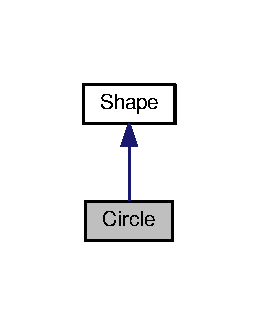
\includegraphics[width=124pt]{class_circle__inherit__graph}
\end{center}
\end{figure}


Collaboration diagram for Circle\+:\nopagebreak
\begin{figure}[H]
\begin{center}
\leavevmode
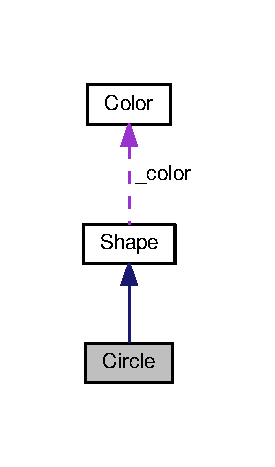
\includegraphics[width=132pt]{class_circle__coll__graph}
\end{center}
\end{figure}
\subsection*{Public Member Functions}
\begin{DoxyCompactItemize}
\item 
\hyperlink{class_circle_a68b0710e21ca715da8bb16c269f8e0ba}{Circle} (const \hyperlink{class_vector2_d}{Vector2D} \&center, const double \&diameter, const \hyperlink{class_color}{Color} \&color=\hyperlink{class_color_a94697e8c9eb81124c5a7c1439e1e7348}{Color\+::get\+Color}(\char`\"{}black\char`\"{}))
\item 
const \hyperlink{class_vector2_d}{Vector2D} \hyperlink{class_circle_a4ed140857e0622e97377f60993c4ec44}{get\+Center} () const
\item 
const double \hyperlink{class_circle_af54e2c9adcf8e6f53ec51560fff849d7}{get\+Diameter} () const
\item 
void \hyperlink{class_circle_a4c2dc8107eab8b562328743cafdddd79}{draw} (\hyperlink{class_drawing_visitor}{Drawing\+Visitor} $\ast$visitor) const
\item 
\hyperlink{class_circle_a4533a225b6d02699cea4045f47d3c7ff}{operator string} () const
\item 
void \hyperlink{class_circle_a91f2af619cc0465ae297ea88ce3b6c23}{save} (const \hyperlink{class_save_visitor}{Save\+Visitor} $\ast$save\+Visitor, const string \&filename) const
\item 
\hyperlink{class_shape}{Shape} $\ast$ \hyperlink{class_circle_ad3b54b369f44baa1947aa3991f55e068}{translation} (const \hyperlink{class_vector2_d}{Vector2D} \&translation\+Vector) const
\item 
\hyperlink{class_shape}{Shape} $\ast$ \hyperlink{class_circle_a031f188681977c2cf6ba2e80e30fb5ce}{homothety} (const \hyperlink{class_vector2_d}{Vector2D} \&invariant\+Point, const double \&homothety\+Ratio) const
\item 
\hyperlink{class_shape}{Shape} $\ast$ \hyperlink{class_circle_ac676105f9868877ffcecc9c236de10bb}{rotation} (const \hyperlink{class_vector2_d}{Vector2D} \&rotation\+Center, const \hyperlink{class_radian_angle}{Radian\+Angle} \&rotation\+Angle) const
\item 
double \hyperlink{class_circle_a7bfb5ab5c8d4f11890407a2483ad61ee}{get\+Area} () const
\end{DoxyCompactItemize}
\subsection*{Friends}
\begin{DoxyCompactItemize}
\item 
ostream \& \hyperlink{class_circle_aff122891f2c5c68c5016c71add530da2}{operator$<$$<$} (ostream \&os, const \hyperlink{class_circle}{Circle} \&circle)
\end{DoxyCompactItemize}
\subsection*{Additional Inherited Members}


\subsection{Detailed Description}
Represent a \hyperlink{class_circle}{Circle} It\textquotesingle{}s a \hyperlink{class_shape}{Shape} 

\subsection{Constructor \& Destructor Documentation}
\hypertarget{class_circle_a68b0710e21ca715da8bb16c269f8e0ba}{}\label{class_circle_a68b0710e21ca715da8bb16c269f8e0ba} 
\index{Circle@{Circle}!Circle@{Circle}}
\index{Circle@{Circle}!Circle@{Circle}}
\subsubsection{\texorpdfstring{Circle()}{Circle()}}
{\footnotesize\ttfamily Circle\+::\+Circle (\begin{DoxyParamCaption}\item[{const \hyperlink{class_vector2_d}{Vector2D} \&}]{center,  }\item[{const double \&}]{diameter,  }\item[{const \hyperlink{class_color}{Color} \&}]{color = {\ttfamily \hyperlink{class_color_a94697e8c9eb81124c5a7c1439e1e7348}{Color\+::get\+Color}(\char`\"{}black\char`\"{})} }\end{DoxyParamCaption})}

\hyperlink{class_circle}{Circle} constructor 
\begin{DoxyParams}{Parameters}
{\em center} & The center point of the \hyperlink{class_circle}{Circle} \\
\hline
{\em diameter} & The diameter of the \hyperlink{class_circle}{Circle} \\
\hline
{\em color} & The color of the \hyperlink{class_circle}{Circle} \\
\hline
\end{DoxyParams}


\subsection{Member Function Documentation}
\hypertarget{class_circle_a4c2dc8107eab8b562328743cafdddd79}{}\label{class_circle_a4c2dc8107eab8b562328743cafdddd79} 
\index{Circle@{Circle}!draw@{draw}}
\index{draw@{draw}!Circle@{Circle}}
\subsubsection{\texorpdfstring{draw()}{draw()}}
{\footnotesize\ttfamily void Circle\+::draw (\begin{DoxyParamCaption}\item[{\hyperlink{class_drawing_visitor}{Drawing\+Visitor} $\ast$}]{visitor }\end{DoxyParamCaption}) const\hspace{0.3cm}{\ttfamily [virtual]}}

Draws the \hyperlink{class_circle}{Circle} using a \hyperlink{class_drawing_visitor}{Drawing\+Visitor}. 
\begin{DoxyParams}{Parameters}
{\em visitor} & The \hyperlink{class_drawing_visitor}{Drawing\+Visitor} to use to draw the \hyperlink{class_circle}{Circle}. \\
\hline
\end{DoxyParams}


Implements \hyperlink{class_shape_ae67fc6d39dd33759b65ff6112b21eab7}{Shape}.

\hypertarget{class_circle_a7bfb5ab5c8d4f11890407a2483ad61ee}{}\label{class_circle_a7bfb5ab5c8d4f11890407a2483ad61ee} 
\index{Circle@{Circle}!get\+Area@{get\+Area}}
\index{get\+Area@{get\+Area}!Circle@{Circle}}
\subsubsection{\texorpdfstring{get\+Area()}{getArea()}}
{\footnotesize\ttfamily double Circle\+::get\+Area (\begin{DoxyParamCaption}{ }\end{DoxyParamCaption}) const\hspace{0.3cm}{\ttfamily [virtual]}}

Returns the area of the \hyperlink{class_circle}{Circle}. \begin{DoxyReturn}{Returns}
The area of the \hyperlink{class_circle}{Circle}. 
\end{DoxyReturn}


Implements \hyperlink{class_shape_ad9454ee04617290547e7529180b1beae}{Shape}.

\hypertarget{class_circle_a4ed140857e0622e97377f60993c4ec44}{}\label{class_circle_a4ed140857e0622e97377f60993c4ec44} 
\index{Circle@{Circle}!get\+Center@{get\+Center}}
\index{get\+Center@{get\+Center}!Circle@{Circle}}
\subsubsection{\texorpdfstring{get\+Center()}{getCenter()}}
{\footnotesize\ttfamily const \hyperlink{class_vector2_d}{Vector2D} Circle\+::get\+Center (\begin{DoxyParamCaption}{ }\end{DoxyParamCaption}) const}

Gets the center of the circle \begin{DoxyReturn}{Returns}
\hyperlink{class_vector2_d}{Vector2D} the center of the circle 
\end{DoxyReturn}
\hypertarget{class_circle_af54e2c9adcf8e6f53ec51560fff849d7}{}\label{class_circle_af54e2c9adcf8e6f53ec51560fff849d7} 
\index{Circle@{Circle}!get\+Diameter@{get\+Diameter}}
\index{get\+Diameter@{get\+Diameter}!Circle@{Circle}}
\subsubsection{\texorpdfstring{get\+Diameter()}{getDiameter()}}
{\footnotesize\ttfamily const double Circle\+::get\+Diameter (\begin{DoxyParamCaption}{ }\end{DoxyParamCaption}) const}

Gets the diameter of the circle \begin{DoxyReturn}{Returns}
double the diameter of the circle 
\end{DoxyReturn}
\hypertarget{class_circle_a031f188681977c2cf6ba2e80e30fb5ce}{}\label{class_circle_a031f188681977c2cf6ba2e80e30fb5ce} 
\index{Circle@{Circle}!homothety@{homothety}}
\index{homothety@{homothety}!Circle@{Circle}}
\subsubsection{\texorpdfstring{homothety()}{homothety()}}
{\footnotesize\ttfamily \hyperlink{class_shape}{Shape} $\ast$ Circle\+::homothety (\begin{DoxyParamCaption}\item[{const \hyperlink{class_vector2_d}{Vector2D} \&}]{invariant\+Point,  }\item[{const double \&}]{homothety\+Ratio }\end{DoxyParamCaption}) const\hspace{0.3cm}{\ttfamily [virtual]}}

Apply an homothety on the \hyperlink{class_circle}{Circle}. 
\begin{DoxyParams}{Parameters}
{\em invariant\+Point} & The center of the homothety. \\
\hline
{\em homothety\+Ratio} & The ratio of the homothety. \\
\hline
\end{DoxyParams}
\begin{DoxyReturn}{Returns}
Shape$\ast$ the new circle after homothety 
\end{DoxyReturn}


Implements \hyperlink{class_shape_a91f18af3004ba210db5c91084c50beb9}{Shape}.

\hypertarget{class_circle_a4533a225b6d02699cea4045f47d3c7ff}{}\label{class_circle_a4533a225b6d02699cea4045f47d3c7ff} 
\index{Circle@{Circle}!operator string@{operator string}}
\index{operator string@{operator string}!Circle@{Circle}}
\subsubsection{\texorpdfstring{operator string()}{operator string()}}
{\footnotesize\ttfamily Circle\+::operator string (\begin{DoxyParamCaption}{ }\end{DoxyParamCaption}) const\hspace{0.3cm}{\ttfamily [virtual]}}

Returns a string that represents the \hyperlink{class_circle}{Circle}. \begin{DoxyReturn}{Returns}
The string representing the \hyperlink{class_circle}{Circle}. 
\end{DoxyReturn}


Implements \hyperlink{class_shape_a0d74dcb2db0791b88b92f439bf4a6972}{Shape}.

\hypertarget{class_circle_ac676105f9868877ffcecc9c236de10bb}{}\label{class_circle_ac676105f9868877ffcecc9c236de10bb} 
\index{Circle@{Circle}!rotation@{rotation}}
\index{rotation@{rotation}!Circle@{Circle}}
\subsubsection{\texorpdfstring{rotation()}{rotation()}}
{\footnotesize\ttfamily \hyperlink{class_shape}{Shape} $\ast$ Circle\+::rotation (\begin{DoxyParamCaption}\item[{const \hyperlink{class_vector2_d}{Vector2D} \&}]{rotation\+Center,  }\item[{const \hyperlink{class_radian_angle}{Radian\+Angle} \&}]{rotation\+Angle }\end{DoxyParamCaption}) const\hspace{0.3cm}{\ttfamily [virtual]}}

Rotates the \hyperlink{class_circle}{Circle}. 
\begin{DoxyParams}{Parameters}
{\em rotation\+Center} & The center of the rotation. \\
\hline
{\em rotation\+Angle} & The angle of the rotation. \\
\hline
\end{DoxyParams}
\begin{DoxyReturn}{Returns}
Shape$\ast$ the new circle after rotation 
\end{DoxyReturn}


Implements \hyperlink{class_shape_abfc7a673b8a6d9a4d646dc15c771aa0d}{Shape}.

\hypertarget{class_circle_a91f2af619cc0465ae297ea88ce3b6c23}{}\label{class_circle_a91f2af619cc0465ae297ea88ce3b6c23} 
\index{Circle@{Circle}!save@{save}}
\index{save@{save}!Circle@{Circle}}
\subsubsection{\texorpdfstring{save()}{save()}}
{\footnotesize\ttfamily void Circle\+::save (\begin{DoxyParamCaption}\item[{const \hyperlink{class_save_visitor}{Save\+Visitor} $\ast$}]{save\+Visitor,  }\item[{const string \&}]{filename }\end{DoxyParamCaption}) const\hspace{0.3cm}{\ttfamily [virtual]}}

Saves the \hyperlink{class_circle}{Circle}. 
\begin{DoxyParams}{Parameters}
{\em save\+Visitor} & The \hyperlink{class_save_visitor}{Save\+Visitor} to use to save the \hyperlink{class_circle}{Circle}. \\
\hline
\end{DoxyParams}


Implements \hyperlink{class_shape_ae1477829e1b06aad805b8b76312f87bc}{Shape}.

\hypertarget{class_circle_ad3b54b369f44baa1947aa3991f55e068}{}\label{class_circle_ad3b54b369f44baa1947aa3991f55e068} 
\index{Circle@{Circle}!translation@{translation}}
\index{translation@{translation}!Circle@{Circle}}
\subsubsection{\texorpdfstring{translation()}{translation()}}
{\footnotesize\ttfamily \hyperlink{class_shape}{Shape} $\ast$ Circle\+::translation (\begin{DoxyParamCaption}\item[{const \hyperlink{class_vector2_d}{Vector2D} \&}]{translation\+Vector }\end{DoxyParamCaption}) const\hspace{0.3cm}{\ttfamily [virtual]}}

Translate the \hyperlink{class_circle}{Circle} using a translation vector. 
\begin{DoxyParams}{Parameters}
{\em translation\+Vector} & The translation vector to use for the translation. \\
\hline
\end{DoxyParams}
\begin{DoxyReturn}{Returns}
Shape$\ast$ the new circle after Translation 
\end{DoxyReturn}


Implements \hyperlink{class_shape_ad3daca0d9bedf9aa15b92afab63c1de8}{Shape}.



\subsection{Friends And Related Function Documentation}
\hypertarget{class_circle_aff122891f2c5c68c5016c71add530da2}{}\label{class_circle_aff122891f2c5c68c5016c71add530da2} 
\index{Circle@{Circle}!operator$<$$<$@{operator$<$$<$}}
\index{operator$<$$<$@{operator$<$$<$}!Circle@{Circle}}
\subsubsection{\texorpdfstring{operator$<$$<$}{operator<<}}
{\footnotesize\ttfamily ostream\& operator$<$$<$ (\begin{DoxyParamCaption}\item[{ostream \&}]{os,  }\item[{const \hyperlink{class_circle}{Circle} \&}]{circle }\end{DoxyParamCaption})\hspace{0.3cm}{\ttfamily [friend]}}



The documentation for this class was generated from the following files\+:\begin{DoxyCompactItemize}
\item 
src/\+Shape/\hyperlink{_circle_8hpp}{Circle.\+hpp}\item 
src/\+Shape/\hyperlink{_circle_8cpp}{Circle.\+cpp}\end{DoxyCompactItemize}

\hypertarget{class_circle_creator}{}\section{Circle\+Creator Class Reference}
\label{class_circle_creator}\index{Circle\+Creator@{Circle\+Creator}}


{\ttfamily \#include $<$Circle\+Creator.\+hpp$>$}



Inheritance diagram for Circle\+Creator\+:\nopagebreak
\begin{figure}[H]
\begin{center}
\leavevmode
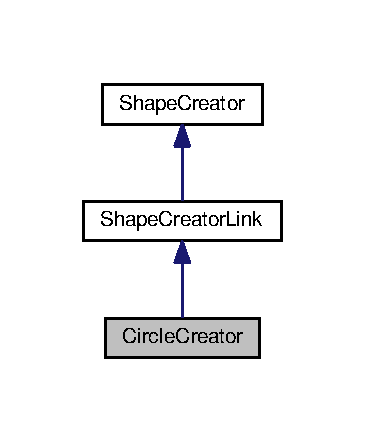
\includegraphics[width=175pt]{class_circle_creator__inherit__graph}
\end{center}
\end{figure}


Collaboration diagram for Circle\+Creator\+:\nopagebreak
\begin{figure}[H]
\begin{center}
\leavevmode
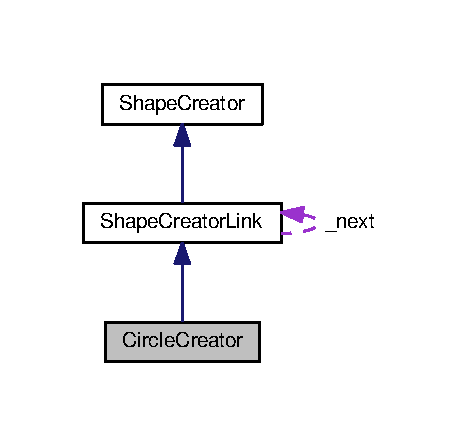
\includegraphics[width=221pt]{class_circle_creator__coll__graph}
\end{center}
\end{figure}
\subsection*{Public Member Functions}
\begin{DoxyCompactItemize}
\item 
\hyperlink{class_circle_creator_a549730b5da4a9ebc7a814ef823683246}{Circle\+Creator} (\hyperlink{class_shape_creator_link}{Shape\+Creator\+Link} $\ast$next)
\item 
virtual \hyperlink{class_shape}{Shape} $\ast$ \hyperlink{class_circle_creator_ae77dd120e2521fdfb2e002228a1f0c25}{create\+Shape\+Spe} (const string \&shape\+String) const
\end{DoxyCompactItemize}
\subsection*{Additional Inherited Members}


\subsection{Detailed Description}
Class \hyperlink{class_circle_creator}{Circle\+Creator} Link of the C\+OR for build \hyperlink{class_circle}{Circle} 

\subsection{Constructor \& Destructor Documentation}
\hypertarget{class_circle_creator_a549730b5da4a9ebc7a814ef823683246}{}\label{class_circle_creator_a549730b5da4a9ebc7a814ef823683246} 
\index{Circle\+Creator@{Circle\+Creator}!Circle\+Creator@{Circle\+Creator}}
\index{Circle\+Creator@{Circle\+Creator}!Circle\+Creator@{Circle\+Creator}}
\subsubsection{\texorpdfstring{Circle\+Creator()}{CircleCreator()}}
{\footnotesize\ttfamily Circle\+Creator\+::\+Circle\+Creator (\begin{DoxyParamCaption}\item[{\hyperlink{class_shape_creator_link}{Shape\+Creator\+Link} $\ast$}]{next }\end{DoxyParamCaption})}

Constructor of \hyperlink{class_circle_creator}{Circle\+Creator} 
\begin{DoxyParams}{Parameters}
{\em next} & The next \hyperlink{class_shape_creator_link}{Shape\+Creator\+Link} if this one fails \\
\hline
\end{DoxyParams}


\subsection{Member Function Documentation}
\hypertarget{class_circle_creator_ae77dd120e2521fdfb2e002228a1f0c25}{}\label{class_circle_creator_ae77dd120e2521fdfb2e002228a1f0c25} 
\index{Circle\+Creator@{Circle\+Creator}!create\+Shape\+Spe@{create\+Shape\+Spe}}
\index{create\+Shape\+Spe@{create\+Shape\+Spe}!Circle\+Creator@{Circle\+Creator}}
\subsubsection{\texorpdfstring{create\+Shape\+Spe()}{createShapeSpe()}}
{\footnotesize\ttfamily \hyperlink{class_shape}{Shape} $\ast$ Circle\+Creator\+::create\+Shape\+Spe (\begin{DoxyParamCaption}\item[{const string \&}]{shape\+String }\end{DoxyParamCaption}) const\hspace{0.3cm}{\ttfamily [virtual]}}

Try to create a \hyperlink{class_circle}{Circle} with the string 
\begin{DoxyParams}{Parameters}
{\em shape\+String} & The string with informations of the shape \\
\hline
\end{DoxyParams}
\begin{DoxyReturn}{Returns}
The Shape$\ast$ wich were created 
\end{DoxyReturn}


Implements \hyperlink{class_shape_creator_link_a036ecc845946d23b36335e9077308bcf}{Shape\+Creator\+Link}.



The documentation for this class was generated from the following files\+:\begin{DoxyCompactItemize}
\item 
src/\+Loader/\hyperlink{_circle_creator_8hpp}{Circle\+Creator.\+hpp}\item 
src/\+Loader/\hyperlink{_circle_creator_8cpp}{Circle\+Creator.\+cpp}\end{DoxyCompactItemize}

\hypertarget{class_color}{}\section{Color Class Reference}
\label{class_color}\index{Color@{Color}}


{\ttfamily \#include $<$Color.\+hpp$>$}

\subsection*{Public Member Functions}
\begin{DoxyCompactItemize}
\item 
\hyperlink{class_color_a0787459fe72580ad9b96a774b1da4c06}{Color} (unsigned char red, unsigned char green, unsigned char blue)
\item 
unsigned char \hyperlink{class_color_a366040ee493dc797f3877c747f70245e}{get\+Red} () const
\item 
unsigned char \hyperlink{class_color_ae97f0bb0f55f82c2e824899d9f8f60ad}{get\+Green} () const
\item 
unsigned char \hyperlink{class_color_afda694abe0a33c924daf178603f44752}{get\+Blue} () const
\item 
\hyperlink{class_color_ac245c9d05bd9409245905b6f15c30f1a}{operator string} () const
\end{DoxyCompactItemize}
\subsection*{Static Public Member Functions}
\begin{DoxyCompactItemize}
\item 
static void \hyperlink{class_color_aba1211bd466bce64d3076af2a55d9785}{init\+Color\+Map} ()
\item 
static \hyperlink{class_color}{Color} \hyperlink{class_color_a94697e8c9eb81124c5a7c1439e1e7348}{get\+Color} (const string \&color)
\end{DoxyCompactItemize}
\subsection*{Friends}
\begin{DoxyCompactItemize}
\item 
ostream \& \hyperlink{class_color_aaa4c7d27cb5d200e5d58e49962d9d9e8}{operator$<$$<$} (ostream \&os, const \hyperlink{class_color}{Color} \&color)
\end{DoxyCompactItemize}


\subsection{Detailed Description}
Represents R\+GB \hyperlink{class_color}{Color} 

\subsection{Constructor \& Destructor Documentation}
\hypertarget{class_color_a0787459fe72580ad9b96a774b1da4c06}{}\label{class_color_a0787459fe72580ad9b96a774b1da4c06} 
\index{Color@{Color}!Color@{Color}}
\index{Color@{Color}!Color@{Color}}
\subsubsection{\texorpdfstring{Color()}{Color()}}
{\footnotesize\ttfamily Color\+::\+Color (\begin{DoxyParamCaption}\item[{unsigned char}]{red,  }\item[{unsigned char}]{green,  }\item[{unsigned char}]{blue }\end{DoxyParamCaption})}

Constructor for \hyperlink{class_color}{Color} 
\begin{DoxyParams}{Parameters}
{\em red} & unsigned char for red intensity \\
\hline
{\em green} & unsigned char for green intensity \\
\hline
{\em blue} & unsigned char for blue intensity \\
\hline
\end{DoxyParams}


\subsection{Member Function Documentation}
\hypertarget{class_color_afda694abe0a33c924daf178603f44752}{}\label{class_color_afda694abe0a33c924daf178603f44752} 
\index{Color@{Color}!get\+Blue@{get\+Blue}}
\index{get\+Blue@{get\+Blue}!Color@{Color}}
\subsubsection{\texorpdfstring{get\+Blue()}{getBlue()}}
{\footnotesize\ttfamily unsigned char Color\+::get\+Blue (\begin{DoxyParamCaption}{ }\end{DoxyParamCaption}) const}

Gets \+\_\+blue intensity \begin{DoxyReturn}{Returns}
blue intensity 
\end{DoxyReturn}
\hypertarget{class_color_a94697e8c9eb81124c5a7c1439e1e7348}{}\label{class_color_a94697e8c9eb81124c5a7c1439e1e7348} 
\index{Color@{Color}!get\+Color@{get\+Color}}
\index{get\+Color@{get\+Color}!Color@{Color}}
\subsubsection{\texorpdfstring{get\+Color()}{getColor()}}
{\footnotesize\ttfamily \hyperlink{class_color}{Color} Color\+::get\+Color (\begin{DoxyParamCaption}\item[{const string \&}]{color }\end{DoxyParamCaption})\hspace{0.3cm}{\ttfamily [static]}}

Gets color in map with a string 
\begin{DoxyParams}{Parameters}
{\em color} & string of the color \\
\hline
\end{DoxyParams}

\begin{DoxyExceptions}{Exceptions}
{\em \hyperlink{class_utils_exception}{Utils\+Exception}} & When color isn\textquotesingle{}t found in the array of colors \\
\hline
\end{DoxyExceptions}
\begin{DoxyReturn}{Returns}
The corresponding \hyperlink{class_color}{Color} object 
\end{DoxyReturn}
\hypertarget{class_color_ae97f0bb0f55f82c2e824899d9f8f60ad}{}\label{class_color_ae97f0bb0f55f82c2e824899d9f8f60ad} 
\index{Color@{Color}!get\+Green@{get\+Green}}
\index{get\+Green@{get\+Green}!Color@{Color}}
\subsubsection{\texorpdfstring{get\+Green()}{getGreen()}}
{\footnotesize\ttfamily unsigned char Color\+::get\+Green (\begin{DoxyParamCaption}{ }\end{DoxyParamCaption}) const}

Gets \+\_\+green intensity \begin{DoxyReturn}{Returns}
green intensity 
\end{DoxyReturn}
\hypertarget{class_color_a366040ee493dc797f3877c747f70245e}{}\label{class_color_a366040ee493dc797f3877c747f70245e} 
\index{Color@{Color}!get\+Red@{get\+Red}}
\index{get\+Red@{get\+Red}!Color@{Color}}
\subsubsection{\texorpdfstring{get\+Red()}{getRed()}}
{\footnotesize\ttfamily unsigned char Color\+::get\+Red (\begin{DoxyParamCaption}{ }\end{DoxyParamCaption}) const}

Gets \+\_\+red intensity \begin{DoxyReturn}{Returns}
red intensity 
\end{DoxyReturn}
\hypertarget{class_color_aba1211bd466bce64d3076af2a55d9785}{}\label{class_color_aba1211bd466bce64d3076af2a55d9785} 
\index{Color@{Color}!init\+Color\+Map@{init\+Color\+Map}}
\index{init\+Color\+Map@{init\+Color\+Map}!Color@{Color}}
\subsubsection{\texorpdfstring{init\+Color\+Map()}{initColorMap()}}
{\footnotesize\ttfamily void Color\+::init\+Color\+Map (\begin{DoxyParamCaption}{ }\end{DoxyParamCaption})\hspace{0.3cm}{\ttfamily [static]}}

Initialize map of color \hypertarget{class_color_ac245c9d05bd9409245905b6f15c30f1a}{}\label{class_color_ac245c9d05bd9409245905b6f15c30f1a} 
\index{Color@{Color}!operator string@{operator string}}
\index{operator string@{operator string}!Color@{Color}}
\subsubsection{\texorpdfstring{operator string()}{operator string()}}
{\footnotesize\ttfamily Color\+::operator string (\begin{DoxyParamCaption}{ }\end{DoxyParamCaption}) const}

Operator cast to string 

\subsection{Friends And Related Function Documentation}
\hypertarget{class_color_aaa4c7d27cb5d200e5d58e49962d9d9e8}{}\label{class_color_aaa4c7d27cb5d200e5d58e49962d9d9e8} 
\index{Color@{Color}!operator$<$$<$@{operator$<$$<$}}
\index{operator$<$$<$@{operator$<$$<$}!Color@{Color}}
\subsubsection{\texorpdfstring{operator$<$$<$}{operator<<}}
{\footnotesize\ttfamily ostream\& operator$<$$<$ (\begin{DoxyParamCaption}\item[{ostream \&}]{os,  }\item[{const \hyperlink{class_color}{Color} \&}]{color }\end{DoxyParamCaption})\hspace{0.3cm}{\ttfamily [friend]}}



The documentation for this class was generated from the following files\+:\begin{DoxyCompactItemize}
\item 
src/\+Utils/\hyperlink{_color_8hpp}{Color.\+hpp}\item 
src/\+Utils/\hyperlink{_color_8cpp}{Color.\+cpp}\end{DoxyCompactItemize}

\hypertarget{class_composed_shape}{}\section{Composed\+Shape Class Reference}
\label{class_composed_shape}\index{Composed\+Shape@{Composed\+Shape}}


{\ttfamily \#include $<$Composed\+Shape.\+hpp$>$}



Inheritance diagram for Composed\+Shape\+:\nopagebreak
\begin{figure}[H]
\begin{center}
\leavevmode
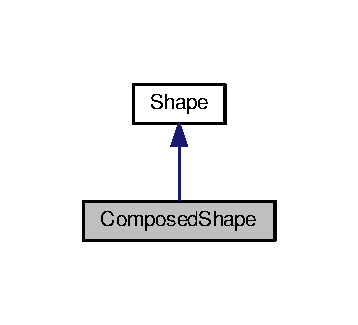
\includegraphics[width=172pt]{class_composed_shape__inherit__graph}
\end{center}
\end{figure}


Collaboration diagram for Composed\+Shape\+:\nopagebreak
\begin{figure}[H]
\begin{center}
\leavevmode
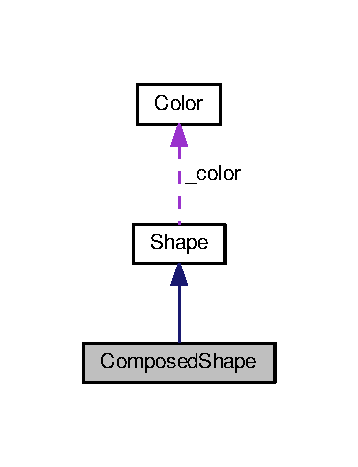
\includegraphics[width=172pt]{class_composed_shape__coll__graph}
\end{center}
\end{figure}
\subsection*{Public Member Functions}
\begin{DoxyCompactItemize}
\item 
\hyperlink{class_composed_shape_a048c0d943a560bba5f5b4c9d9a18afc9}{Composed\+Shape} (\hyperlink{class_color}{Color} color=\hyperlink{class_color_a94697e8c9eb81124c5a7c1439e1e7348}{Color\+::get\+Color}(\char`\"{}black\char`\"{}))
\item 
void \hyperlink{class_composed_shape_a5f78e498ae77eeefc868d28ae8c8aa99}{add\+Shape} (\hyperlink{class_shape}{Shape} $\ast$shape)
\item 
void \hyperlink{class_composed_shape_a30f69734aa983bca56574ff4e5fd1723}{draw} (\hyperlink{class_drawing_visitor}{Drawing\+Visitor} $\ast$visitor) const
\item 
\hyperlink{class_composed_shape_aef491963b0e58209d1921973f2711c94}{operator string} () const
\item 
void \hyperlink{class_composed_shape_af189684eb5328b2fc13c694d7e637ff8}{save} (const \hyperlink{class_save_visitor}{Save\+Visitor} $\ast$save\+Visitor, const string \&filename) const
\item 
\hyperlink{class_shape}{Shape} $\ast$ \hyperlink{class_composed_shape_a31337a3fc33ac1fb929edbb6ff485dcc}{translation} (const \hyperlink{class_vector2_d}{Vector2D} \&translation\+Vector) const
\item 
\hyperlink{class_shape}{Shape} $\ast$ \hyperlink{class_composed_shape_acff645310f05924aaf66b0de71b2307a}{homothety} (const \hyperlink{class_vector2_d}{Vector2D} \&invariant\+Point, const double \&homothety\+Ratio) const
\item 
\hyperlink{class_shape}{Shape} $\ast$ \hyperlink{class_composed_shape_a9c4f0561d631b20c6cd56348d41a14dd}{rotation} (const \hyperlink{class_vector2_d}{Vector2D} \&rotation\+Center, const \hyperlink{class_radian_angle}{Radian\+Angle} \&rotation\+Angle) const
\item 
double \hyperlink{class_composed_shape_a89b3457e1699afeb86805afad627d2c7}{get\+Area} () const
\item 
int \hyperlink{class_composed_shape_ab33696ffeb5f3840cf0c5b75c8911787}{get\+Shape\+Number} () const
\item 
const \hyperlink{class_shape}{Shape} $\ast$ \hyperlink{class_composed_shape_a144d7d70317e5123f081d36689254ea8}{get\+Shape} (unsigned int i) const
\end{DoxyCompactItemize}
\subsection*{Friends}
\begin{DoxyCompactItemize}
\item 
ostream \& \hyperlink{class_composed_shape_a68ff1b04d83134ec6f6e949b45b63016}{operator$<$$<$} (ostream \&os, const \hyperlink{class_composed_shape}{Composed\+Shape} \&composed\+Shape)
\end{DoxyCompactItemize}
\subsection*{Additional Inherited Members}


\subsection{Detailed Description}
Represent a \hyperlink{class_composed_shape}{Composed\+Shape} It\textquotesingle{}s a \hyperlink{class_shape}{Shape} 

\subsection{Constructor \& Destructor Documentation}
\hypertarget{class_composed_shape_a048c0d943a560bba5f5b4c9d9a18afc9}{}\label{class_composed_shape_a048c0d943a560bba5f5b4c9d9a18afc9} 
\index{Composed\+Shape@{Composed\+Shape}!Composed\+Shape@{Composed\+Shape}}
\index{Composed\+Shape@{Composed\+Shape}!Composed\+Shape@{Composed\+Shape}}
\subsubsection{\texorpdfstring{Composed\+Shape()}{ComposedShape()}}
{\footnotesize\ttfamily Composed\+Shape\+::\+Composed\+Shape (\begin{DoxyParamCaption}\item[{\hyperlink{class_color}{Color}}]{color = {\ttfamily \hyperlink{class_color_a94697e8c9eb81124c5a7c1439e1e7348}{Color\+::get\+Color}(\char`\"{}black\char`\"{})} }\end{DoxyParamCaption})}

\hyperlink{class_composed_shape}{Composed\+Shape} constructors 

\subsection{Member Function Documentation}
\hypertarget{class_composed_shape_a5f78e498ae77eeefc868d28ae8c8aa99}{}\label{class_composed_shape_a5f78e498ae77eeefc868d28ae8c8aa99} 
\index{Composed\+Shape@{Composed\+Shape}!add\+Shape@{add\+Shape}}
\index{add\+Shape@{add\+Shape}!Composed\+Shape@{Composed\+Shape}}
\subsubsection{\texorpdfstring{add\+Shape()}{addShape()}}
{\footnotesize\ttfamily void Composed\+Shape\+::add\+Shape (\begin{DoxyParamCaption}\item[{\hyperlink{class_shape}{Shape} $\ast$}]{shape }\end{DoxyParamCaption})}

Function to add a point on the \hyperlink{class_composed_shape}{Composed\+Shape} 
\begin{DoxyParams}{Parameters}
{\em point} & point to add \\
\hline
\end{DoxyParams}
\hypertarget{class_composed_shape_a30f69734aa983bca56574ff4e5fd1723}{}\label{class_composed_shape_a30f69734aa983bca56574ff4e5fd1723} 
\index{Composed\+Shape@{Composed\+Shape}!draw@{draw}}
\index{draw@{draw}!Composed\+Shape@{Composed\+Shape}}
\subsubsection{\texorpdfstring{draw()}{draw()}}
{\footnotesize\ttfamily void Composed\+Shape\+::draw (\begin{DoxyParamCaption}\item[{\hyperlink{class_drawing_visitor}{Drawing\+Visitor} $\ast$}]{visitor }\end{DoxyParamCaption}) const\hspace{0.3cm}{\ttfamily [virtual]}}

Draws the \hyperlink{class_composed_shape}{Composed\+Shape} using a \hyperlink{class_drawing_visitor}{Drawing\+Visitor}. 
\begin{DoxyParams}{Parameters}
{\em visitor} & The \hyperlink{class_drawing_visitor}{Drawing\+Visitor} to use to draw the \hyperlink{class_composed_shape}{Composed\+Shape}. \\
\hline
\end{DoxyParams}


Implements \hyperlink{class_shape_ae67fc6d39dd33759b65ff6112b21eab7}{Shape}.

\hypertarget{class_composed_shape_a89b3457e1699afeb86805afad627d2c7}{}\label{class_composed_shape_a89b3457e1699afeb86805afad627d2c7} 
\index{Composed\+Shape@{Composed\+Shape}!get\+Area@{get\+Area}}
\index{get\+Area@{get\+Area}!Composed\+Shape@{Composed\+Shape}}
\subsubsection{\texorpdfstring{get\+Area()}{getArea()}}
{\footnotesize\ttfamily double Composed\+Shape\+::get\+Area (\begin{DoxyParamCaption}{ }\end{DoxyParamCaption}) const\hspace{0.3cm}{\ttfamily [virtual]}}

Returns the area of the \hyperlink{class_composed_shape}{Composed\+Shape}. \begin{DoxyReturn}{Returns}
The area of the \hyperlink{class_composed_shape}{Composed\+Shape}. 
\end{DoxyReturn}


Implements \hyperlink{class_shape_ad9454ee04617290547e7529180b1beae}{Shape}.

\hypertarget{class_composed_shape_a144d7d70317e5123f081d36689254ea8}{}\label{class_composed_shape_a144d7d70317e5123f081d36689254ea8} 
\index{Composed\+Shape@{Composed\+Shape}!get\+Shape@{get\+Shape}}
\index{get\+Shape@{get\+Shape}!Composed\+Shape@{Composed\+Shape}}
\subsubsection{\texorpdfstring{get\+Shape()}{getShape()}}
{\footnotesize\ttfamily const \hyperlink{class_shape}{Shape} $\ast$ Composed\+Shape\+::get\+Shape (\begin{DoxyParamCaption}\item[{unsigned int}]{i }\end{DoxyParamCaption}) const}

Returns the i-\/th shape in this \hyperlink{class_composed_shape}{Composed\+Shape} \begin{DoxyReturn}{Returns}
The i-\/th shape in this \hyperlink{class_composed_shape}{Composed\+Shape} 
\end{DoxyReturn}

\begin{DoxyExceptions}{Exceptions}
{\em Shape\+Exception} & if the index is wrong. \\
\hline
\end{DoxyExceptions}
\hypertarget{class_composed_shape_ab33696ffeb5f3840cf0c5b75c8911787}{}\label{class_composed_shape_ab33696ffeb5f3840cf0c5b75c8911787} 
\index{Composed\+Shape@{Composed\+Shape}!get\+Shape\+Number@{get\+Shape\+Number}}
\index{get\+Shape\+Number@{get\+Shape\+Number}!Composed\+Shape@{Composed\+Shape}}
\subsubsection{\texorpdfstring{get\+Shape\+Number()}{getShapeNumber()}}
{\footnotesize\ttfamily int Composed\+Shape\+::get\+Shape\+Number (\begin{DoxyParamCaption}{ }\end{DoxyParamCaption}) const}

Returns the number of Shapes composing this \hyperlink{class_composed_shape}{Composed\+Shape}. \begin{DoxyReturn}{Returns}
The number of shapes composing this \hyperlink{class_composed_shape}{Composed\+Shape}. 
\end{DoxyReturn}
\hypertarget{class_composed_shape_acff645310f05924aaf66b0de71b2307a}{}\label{class_composed_shape_acff645310f05924aaf66b0de71b2307a} 
\index{Composed\+Shape@{Composed\+Shape}!homothety@{homothety}}
\index{homothety@{homothety}!Composed\+Shape@{Composed\+Shape}}
\subsubsection{\texorpdfstring{homothety()}{homothety()}}
{\footnotesize\ttfamily \hyperlink{class_shape}{Shape} $\ast$ Composed\+Shape\+::homothety (\begin{DoxyParamCaption}\item[{const \hyperlink{class_vector2_d}{Vector2D} \&}]{invariant\+Point,  }\item[{const double \&}]{homothety\+Ratio }\end{DoxyParamCaption}) const\hspace{0.3cm}{\ttfamily [virtual]}}

Apply an homothety on the \hyperlink{class_composed_shape}{Composed\+Shape}. 
\begin{DoxyParams}{Parameters}
{\em invariant\+Point} & The center of the homothety. \\
\hline
{\em homothety\+Ratio} & The ratio of the homothety. \\
\hline
\end{DoxyParams}
\begin{DoxyReturn}{Returns}
Shape$\ast$ the new \hyperlink{class_composed_shape}{Composed\+Shape} after homothety 
\end{DoxyReturn}


Implements \hyperlink{class_shape_a91f18af3004ba210db5c91084c50beb9}{Shape}.

\hypertarget{class_composed_shape_aef491963b0e58209d1921973f2711c94}{}\label{class_composed_shape_aef491963b0e58209d1921973f2711c94} 
\index{Composed\+Shape@{Composed\+Shape}!operator string@{operator string}}
\index{operator string@{operator string}!Composed\+Shape@{Composed\+Shape}}
\subsubsection{\texorpdfstring{operator string()}{operator string()}}
{\footnotesize\ttfamily Composed\+Shape\+::operator string (\begin{DoxyParamCaption}{ }\end{DoxyParamCaption}) const\hspace{0.3cm}{\ttfamily [virtual]}}

Returns a string that represents the \hyperlink{class_composed_shape}{Composed\+Shape}. \begin{DoxyReturn}{Returns}
The string representing the \hyperlink{class_composed_shape}{Composed\+Shape}. 
\end{DoxyReturn}


Implements \hyperlink{class_shape_a0d74dcb2db0791b88b92f439bf4a6972}{Shape}.

\hypertarget{class_composed_shape_a9c4f0561d631b20c6cd56348d41a14dd}{}\label{class_composed_shape_a9c4f0561d631b20c6cd56348d41a14dd} 
\index{Composed\+Shape@{Composed\+Shape}!rotation@{rotation}}
\index{rotation@{rotation}!Composed\+Shape@{Composed\+Shape}}
\subsubsection{\texorpdfstring{rotation()}{rotation()}}
{\footnotesize\ttfamily \hyperlink{class_shape}{Shape} $\ast$ Composed\+Shape\+::rotation (\begin{DoxyParamCaption}\item[{const \hyperlink{class_vector2_d}{Vector2D} \&}]{rotation\+Center,  }\item[{const \hyperlink{class_radian_angle}{Radian\+Angle} \&}]{rotation\+Angle }\end{DoxyParamCaption}) const\hspace{0.3cm}{\ttfamily [virtual]}}

Rotates the \hyperlink{class_composed_shape}{Composed\+Shape}. 
\begin{DoxyParams}{Parameters}
{\em rotation\+Center} & The center of the rotation. \\
\hline
{\em rotation\+Angle} & The angle of the rotation. \\
\hline
\end{DoxyParams}
\begin{DoxyReturn}{Returns}
Shape$\ast$ the new \hyperlink{class_composed_shape}{Composed\+Shape} after rotation 
\end{DoxyReturn}


Implements \hyperlink{class_shape_abfc7a673b8a6d9a4d646dc15c771aa0d}{Shape}.

\hypertarget{class_composed_shape_af189684eb5328b2fc13c694d7e637ff8}{}\label{class_composed_shape_af189684eb5328b2fc13c694d7e637ff8} 
\index{Composed\+Shape@{Composed\+Shape}!save@{save}}
\index{save@{save}!Composed\+Shape@{Composed\+Shape}}
\subsubsection{\texorpdfstring{save()}{save()}}
{\footnotesize\ttfamily void Composed\+Shape\+::save (\begin{DoxyParamCaption}\item[{const \hyperlink{class_save_visitor}{Save\+Visitor} $\ast$}]{save\+Visitor,  }\item[{const string \&}]{filename }\end{DoxyParamCaption}) const\hspace{0.3cm}{\ttfamily [virtual]}}

Saves the \hyperlink{class_composed_shape}{Composed\+Shape}. 
\begin{DoxyParams}{Parameters}
{\em save\+Visitor} & The \hyperlink{class_save_visitor}{Save\+Visitor} to use to save the \hyperlink{class_composed_shape}{Composed\+Shape}. \\
\hline
\end{DoxyParams}


Implements \hyperlink{class_shape_ae1477829e1b06aad805b8b76312f87bc}{Shape}.

\hypertarget{class_composed_shape_a31337a3fc33ac1fb929edbb6ff485dcc}{}\label{class_composed_shape_a31337a3fc33ac1fb929edbb6ff485dcc} 
\index{Composed\+Shape@{Composed\+Shape}!translation@{translation}}
\index{translation@{translation}!Composed\+Shape@{Composed\+Shape}}
\subsubsection{\texorpdfstring{translation()}{translation()}}
{\footnotesize\ttfamily \hyperlink{class_shape}{Shape} $\ast$ Composed\+Shape\+::translation (\begin{DoxyParamCaption}\item[{const \hyperlink{class_vector2_d}{Vector2D} \&}]{translation\+Vector }\end{DoxyParamCaption}) const\hspace{0.3cm}{\ttfamily [virtual]}}

Translate the \hyperlink{class_composed_shape}{Composed\+Shape} using a translation vector. 
\begin{DoxyParams}{Parameters}
{\em translation\+Vector} & The translation vector to use for the translation. \\
\hline
\end{DoxyParams}
\begin{DoxyReturn}{Returns}
Shape$\ast$ the new \hyperlink{class_composed_shape}{Composed\+Shape} after Translation 
\end{DoxyReturn}


Implements \hyperlink{class_shape_ad3daca0d9bedf9aa15b92afab63c1de8}{Shape}.



\subsection{Friends And Related Function Documentation}
\hypertarget{class_composed_shape_a68ff1b04d83134ec6f6e949b45b63016}{}\label{class_composed_shape_a68ff1b04d83134ec6f6e949b45b63016} 
\index{Composed\+Shape@{Composed\+Shape}!operator$<$$<$@{operator$<$$<$}}
\index{operator$<$$<$@{operator$<$$<$}!Composed\+Shape@{Composed\+Shape}}
\subsubsection{\texorpdfstring{operator$<$$<$}{operator<<}}
{\footnotesize\ttfamily ostream\& operator$<$$<$ (\begin{DoxyParamCaption}\item[{ostream \&}]{os,  }\item[{const \hyperlink{class_composed_shape}{Composed\+Shape} \&}]{composed\+Shape }\end{DoxyParamCaption})\hspace{0.3cm}{\ttfamily [friend]}}



The documentation for this class was generated from the following files\+:\begin{DoxyCompactItemize}
\item 
src/\+Shape/\hyperlink{_composed_shape_8hpp}{Composed\+Shape.\+hpp}\item 
src/\+Shape/\hyperlink{_composed_shape_8cpp}{Composed\+Shape.\+cpp}\end{DoxyCompactItemize}

\hypertarget{class_composed_shape_creator}{}\section{Composed\+Shape\+Creator Class Reference}
\label{class_composed_shape_creator}\index{Composed\+Shape\+Creator@{Composed\+Shape\+Creator}}


{\ttfamily \#include $<$Composed\+Shape\+Creator.\+hpp$>$}



Inheritance diagram for Composed\+Shape\+Creator\+:\nopagebreak
\begin{figure}[H]
\begin{center}
\leavevmode
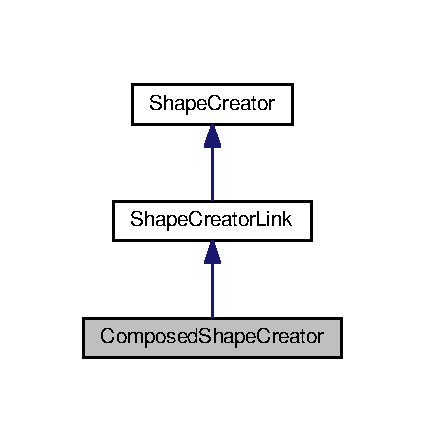
\includegraphics[width=204pt]{class_composed_shape_creator__inherit__graph}
\end{center}
\end{figure}


Collaboration diagram for Composed\+Shape\+Creator\+:\nopagebreak
\begin{figure}[H]
\begin{center}
\leavevmode
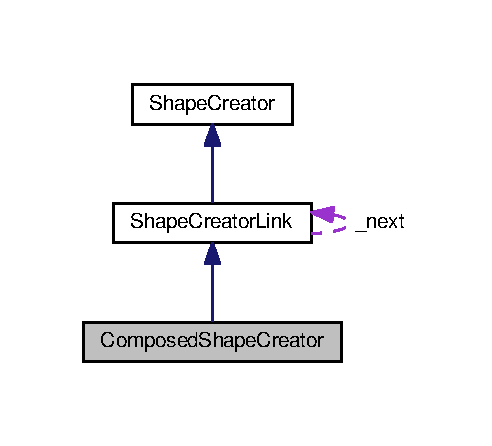
\includegraphics[width=236pt]{class_composed_shape_creator__coll__graph}
\end{center}
\end{figure}
\subsection*{Public Member Functions}
\begin{DoxyCompactItemize}
\item 
\hyperlink{class_composed_shape_creator_a6fc84212ed85e2a63c748faceb464a58}{Composed\+Shape\+Creator} (\hyperlink{class_shape_creator_link}{Shape\+Creator\+Link} $\ast$next)
\item 
virtual \hyperlink{class_shape}{Shape} $\ast$ \hyperlink{class_composed_shape_creator_a5a1ebce5d0d7509923e70d507dc57ff2}{create\+Shape\+Spe} (const string \&shape\+String) const
\end{DoxyCompactItemize}
\subsection*{Additional Inherited Members}


\subsection{Detailed Description}
Class \hyperlink{class_composed_shape_creator}{Composed\+Shape\+Creator} Link of the C\+OR for build \hyperlink{class_composed_shape}{Composed\+Shape} 

\subsection{Constructor \& Destructor Documentation}
\hypertarget{class_composed_shape_creator_a6fc84212ed85e2a63c748faceb464a58}{}\label{class_composed_shape_creator_a6fc84212ed85e2a63c748faceb464a58} 
\index{Composed\+Shape\+Creator@{Composed\+Shape\+Creator}!Composed\+Shape\+Creator@{Composed\+Shape\+Creator}}
\index{Composed\+Shape\+Creator@{Composed\+Shape\+Creator}!Composed\+Shape\+Creator@{Composed\+Shape\+Creator}}
\subsubsection{\texorpdfstring{Composed\+Shape\+Creator()}{ComposedShapeCreator()}}
{\footnotesize\ttfamily Composed\+Shape\+Creator\+::\+Composed\+Shape\+Creator (\begin{DoxyParamCaption}\item[{\hyperlink{class_shape_creator_link}{Shape\+Creator\+Link} $\ast$}]{next }\end{DoxyParamCaption})}

Constructor of \hyperlink{class_composed_shape_creator}{Composed\+Shape\+Creator} 
\begin{DoxyParams}{Parameters}
{\em next} & The next \hyperlink{class_shape_creator_link}{Shape\+Creator\+Link} if this one fails \\
\hline
\end{DoxyParams}


\subsection{Member Function Documentation}
\hypertarget{class_composed_shape_creator_a5a1ebce5d0d7509923e70d507dc57ff2}{}\label{class_composed_shape_creator_a5a1ebce5d0d7509923e70d507dc57ff2} 
\index{Composed\+Shape\+Creator@{Composed\+Shape\+Creator}!create\+Shape\+Spe@{create\+Shape\+Spe}}
\index{create\+Shape\+Spe@{create\+Shape\+Spe}!Composed\+Shape\+Creator@{Composed\+Shape\+Creator}}
\subsubsection{\texorpdfstring{create\+Shape\+Spe()}{createShapeSpe()}}
{\footnotesize\ttfamily \hyperlink{class_shape}{Shape} $\ast$ Composed\+Shape\+Creator\+::create\+Shape\+Spe (\begin{DoxyParamCaption}\item[{const string \&}]{shape\+String }\end{DoxyParamCaption}) const\hspace{0.3cm}{\ttfamily [virtual]}}

Try to create a \hyperlink{class_composed_shape}{Composed\+Shape} with the string 
\begin{DoxyParams}{Parameters}
{\em shape\+String} & the string with informations of the shape \\
\hline
\end{DoxyParams}
\begin{DoxyReturn}{Returns}
The Shape$\ast$ wich were created 
\end{DoxyReturn}


Implements \hyperlink{class_shape_creator_link_a036ecc845946d23b36335e9077308bcf}{Shape\+Creator\+Link}.



The documentation for this class was generated from the following files\+:\begin{DoxyCompactItemize}
\item 
src/\+Loader/\hyperlink{_composed_shape_creator_8hpp}{Composed\+Shape\+Creator.\+hpp}\item 
src/\+Loader/\hyperlink{_composed_shape_creator_8cpp}{Composed\+Shape\+Creator.\+cpp}\end{DoxyCompactItemize}

\hypertarget{class_drawing_visitor}{}\section{Drawing\+Visitor Class Reference}
\label{class_drawing_visitor}\index{Drawing\+Visitor@{Drawing\+Visitor}}


{\ttfamily \#include $<$Drawing\+Visitor.\+hpp$>$}



Inheritance diagram for Drawing\+Visitor\+:\nopagebreak
\begin{figure}[H]
\begin{center}
\leavevmode
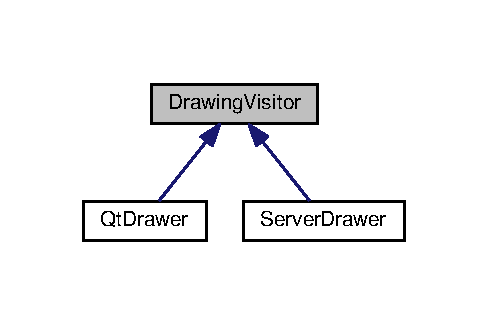
\includegraphics[width=234pt]{class_drawing_visitor__inherit__graph}
\end{center}
\end{figure}
\subsection*{Public Member Functions}
\begin{DoxyCompactItemize}
\item 
virtual void \hyperlink{class_drawing_visitor_a287f6d770c755c1c3bc144fb08b65030}{draw} (const \hyperlink{class_circle}{Circle} $\ast$circle)=0
\item 
virtual void \hyperlink{class_drawing_visitor_a8a95018de31a7e3d7a067c347478ffde}{draw} (const \hyperlink{class_segment}{Segment} $\ast$segment)=0
\item 
virtual void \hyperlink{class_drawing_visitor_a178aa7e1bb9cfbd538d7de0dbfa2d4b1}{draw} (const \hyperlink{class_triangle}{Triangle} $\ast$triangle)=0
\item 
virtual void \hyperlink{class_drawing_visitor_a771a2110a3afe4e87688bddd65657a46}{draw} (const \hyperlink{class_polygon}{Polygon} $\ast$polygon)=0
\item 
virtual void \hyperlink{class_drawing_visitor_ad3d9e3028449f65ea2c405c74c4a55b4}{draw} (const \hyperlink{class_shape}{Shape} $\ast$shape)=0
\end{DoxyCompactItemize}


\subsection{Detailed Description}
The abstract base class for all drawers. 

\subsection{Member Function Documentation}
\hypertarget{class_drawing_visitor_a287f6d770c755c1c3bc144fb08b65030}{}\label{class_drawing_visitor_a287f6d770c755c1c3bc144fb08b65030} 
\index{Drawing\+Visitor@{Drawing\+Visitor}!draw@{draw}}
\index{draw@{draw}!Drawing\+Visitor@{Drawing\+Visitor}}
\subsubsection{\texorpdfstring{draw()}{draw()}\hspace{0.1cm}{\footnotesize\ttfamily [1/5]}}
{\footnotesize\ttfamily virtual void Drawing\+Visitor\+::draw (\begin{DoxyParamCaption}\item[{const \hyperlink{class_circle}{Circle} $\ast$}]{circle }\end{DoxyParamCaption})\hspace{0.3cm}{\ttfamily [pure virtual]}}

Draws the \hyperlink{class_circle}{Circle}. 
\begin{DoxyParams}{Parameters}
{\em circle} & The \hyperlink{class_circle}{Circle} to draw. \\
\hline
\end{DoxyParams}


Implemented in \hyperlink{class_qt_drawer_a1e9a6ad76355f26fc9b41b54b28a04f4}{Qt\+Drawer}, and \hyperlink{class_server_drawer_a70bd94ed93c913b53d689fb8fc5dddc9}{Server\+Drawer}.

\hypertarget{class_drawing_visitor_a8a95018de31a7e3d7a067c347478ffde}{}\label{class_drawing_visitor_a8a95018de31a7e3d7a067c347478ffde} 
\index{Drawing\+Visitor@{Drawing\+Visitor}!draw@{draw}}
\index{draw@{draw}!Drawing\+Visitor@{Drawing\+Visitor}}
\subsubsection{\texorpdfstring{draw()}{draw()}\hspace{0.1cm}{\footnotesize\ttfamily [2/5]}}
{\footnotesize\ttfamily virtual void Drawing\+Visitor\+::draw (\begin{DoxyParamCaption}\item[{const \hyperlink{class_segment}{Segment} $\ast$}]{segment }\end{DoxyParamCaption})\hspace{0.3cm}{\ttfamily [pure virtual]}}

Draws the \hyperlink{class_segment}{Segment}. 
\begin{DoxyParams}{Parameters}
{\em segment} & The \hyperlink{class_segment}{Segment} to draw. \\
\hline
\end{DoxyParams}


Implemented in \hyperlink{class_qt_drawer_afe2f299e83092e1d4676c8b3fd4a3452}{Qt\+Drawer}, and \hyperlink{class_server_drawer_a2bec9e70a1111d59b6c2d7de0908d780}{Server\+Drawer}.

\hypertarget{class_drawing_visitor_a178aa7e1bb9cfbd538d7de0dbfa2d4b1}{}\label{class_drawing_visitor_a178aa7e1bb9cfbd538d7de0dbfa2d4b1} 
\index{Drawing\+Visitor@{Drawing\+Visitor}!draw@{draw}}
\index{draw@{draw}!Drawing\+Visitor@{Drawing\+Visitor}}
\subsubsection{\texorpdfstring{draw()}{draw()}\hspace{0.1cm}{\footnotesize\ttfamily [3/5]}}
{\footnotesize\ttfamily virtual void Drawing\+Visitor\+::draw (\begin{DoxyParamCaption}\item[{const \hyperlink{class_triangle}{Triangle} $\ast$}]{triangle }\end{DoxyParamCaption})\hspace{0.3cm}{\ttfamily [pure virtual]}}

Draws the \hyperlink{class_triangle}{Triangle}. 
\begin{DoxyParams}{Parameters}
{\em triangle} & The \hyperlink{class_triangle}{Triangle} to draw. \\
\hline
\end{DoxyParams}


Implemented in \hyperlink{class_qt_drawer_a6d68080c84447a76b34810ca0330fd2c}{Qt\+Drawer}, and \hyperlink{class_server_drawer_aad913eff7f5c248003ef70ec8c09d2b2}{Server\+Drawer}.

\hypertarget{class_drawing_visitor_a771a2110a3afe4e87688bddd65657a46}{}\label{class_drawing_visitor_a771a2110a3afe4e87688bddd65657a46} 
\index{Drawing\+Visitor@{Drawing\+Visitor}!draw@{draw}}
\index{draw@{draw}!Drawing\+Visitor@{Drawing\+Visitor}}
\subsubsection{\texorpdfstring{draw()}{draw()}\hspace{0.1cm}{\footnotesize\ttfamily [4/5]}}
{\footnotesize\ttfamily virtual void Drawing\+Visitor\+::draw (\begin{DoxyParamCaption}\item[{const \hyperlink{class_polygon}{Polygon} $\ast$}]{polygon }\end{DoxyParamCaption})\hspace{0.3cm}{\ttfamily [pure virtual]}}

Draws the \hyperlink{class_polygon}{Polygon}. 
\begin{DoxyParams}{Parameters}
{\em polygon} & The \hyperlink{class_polygon}{Polygon} to draw. \\
\hline
\end{DoxyParams}


Implemented in \hyperlink{class_qt_drawer_a977cc5f97827eb36063f8429ef044727}{Qt\+Drawer}, and \hyperlink{class_server_drawer_acd973f89e7618d67fcd8db364df0b6bf}{Server\+Drawer}.

\hypertarget{class_drawing_visitor_ad3d9e3028449f65ea2c405c74c4a55b4}{}\label{class_drawing_visitor_ad3d9e3028449f65ea2c405c74c4a55b4} 
\index{Drawing\+Visitor@{Drawing\+Visitor}!draw@{draw}}
\index{draw@{draw}!Drawing\+Visitor@{Drawing\+Visitor}}
\subsubsection{\texorpdfstring{draw()}{draw()}\hspace{0.1cm}{\footnotesize\ttfamily [5/5]}}
{\footnotesize\ttfamily virtual void Drawing\+Visitor\+::draw (\begin{DoxyParamCaption}\item[{const \hyperlink{class_shape}{Shape} $\ast$}]{shape }\end{DoxyParamCaption})\hspace{0.3cm}{\ttfamily [pure virtual]}}

Draws the \hyperlink{class_shape}{Shape}. 
\begin{DoxyParams}{Parameters}
{\em polygon} & The \hyperlink{class_shape}{Shape} to draw. \\
\hline
\end{DoxyParams}


Implemented in \hyperlink{class_qt_drawer_a031e3b3242e341fa6e6fdcbf96b3dbfe}{Qt\+Drawer}, and \hyperlink{class_server_drawer_a071fa49ab9edc71554b32aaaf7422b7f}{Server\+Drawer}.



The documentation for this class was generated from the following file\+:\begin{DoxyCompactItemize}
\item 
src/\+Visitor/\hyperlink{_drawing_visitor_8hpp}{Drawing\+Visitor.\+hpp}\end{DoxyCompactItemize}

\hypertarget{class_geometry_exception}{}\section{Geometry\+Exception Class Reference}
\label{class_geometry_exception}\index{Geometry\+Exception@{Geometry\+Exception}}


{\ttfamily \#include $<$Geometry\+Exception.\+hpp$>$}

\subsection*{Public Member Functions}
\begin{DoxyCompactItemize}
\item 
\hyperlink{class_geometry_exception_a15e945c91a8d6aaa1a2d18edd9f7971f}{Geometry\+Exception} (const string \&message)
\end{DoxyCompactItemize}
\subsection*{Friends}
\begin{DoxyCompactItemize}
\item 
ostream \& \hyperlink{class_geometry_exception_a1a0e9b6dde275e9a72dd6538ab4a7b73}{operator$<$$<$} (ostream \&os, const \hyperlink{class_geometry_exception}{Geometry\+Exception} \&geometry\+Exception)
\end{DoxyCompactItemize}


\subsection{Detailed Description}
Class for hander all geometrique exceptions 

\subsection{Constructor \& Destructor Documentation}
\hypertarget{class_geometry_exception_a15e945c91a8d6aaa1a2d18edd9f7971f}{}\label{class_geometry_exception_a15e945c91a8d6aaa1a2d18edd9f7971f} 
\index{Geometry\+Exception@{Geometry\+Exception}!Geometry\+Exception@{Geometry\+Exception}}
\index{Geometry\+Exception@{Geometry\+Exception}!Geometry\+Exception@{Geometry\+Exception}}
\subsubsection{\texorpdfstring{Geometry\+Exception()}{GeometryException()}}
{\footnotesize\ttfamily Geometry\+Exception\+::\+Geometry\+Exception (\begin{DoxyParamCaption}\item[{const string \&}]{message }\end{DoxyParamCaption})}

Constructor of \hyperlink{class_geometry_exception}{Geometry\+Exception} 
\begin{DoxyParams}{Parameters}
{\em message} & the message to throw \\
\hline
\end{DoxyParams}


\subsection{Friends And Related Function Documentation}
\hypertarget{class_geometry_exception_a1a0e9b6dde275e9a72dd6538ab4a7b73}{}\label{class_geometry_exception_a1a0e9b6dde275e9a72dd6538ab4a7b73} 
\index{Geometry\+Exception@{Geometry\+Exception}!operator$<$$<$@{operator$<$$<$}}
\index{operator$<$$<$@{operator$<$$<$}!Geometry\+Exception@{Geometry\+Exception}}
\subsubsection{\texorpdfstring{operator$<$$<$}{operator<<}}
{\footnotesize\ttfamily ostream\& operator$<$$<$ (\begin{DoxyParamCaption}\item[{ostream \&}]{os,  }\item[{const \hyperlink{class_geometry_exception}{Geometry\+Exception} \&}]{geometry\+Exception }\end{DoxyParamCaption})\hspace{0.3cm}{\ttfamily [friend]}}

Sends a string of excpetion to a stream 
\begin{DoxyParams}{Parameters}
{\em os} & ostream \\
\hline
{\em geometry\+Exception} & \hyperlink{class_geometry_exception}{Geometry\+Exception} have to print \\
\hline
\end{DoxyParams}
\begin{DoxyReturn}{Returns}
ostream to send to the output 
\end{DoxyReturn}


The documentation for this class was generated from the following files\+:\begin{DoxyCompactItemize}
\item 
src/\+Geometry/\hyperlink{_geometry_exception_8hpp}{Geometry\+Exception.\+hpp}\item 
src/\+Geometry/\hyperlink{_geometry_exception_8cpp}{Geometry\+Exception.\+cpp}\end{DoxyCompactItemize}

\hypertarget{class_network_exception}{}\section{Network\+Exception Class Reference}
\label{class_network_exception}\index{Network\+Exception@{Network\+Exception}}


{\ttfamily \#include $<$Network\+Exception.\+hpp$>$}

\subsection*{Public Member Functions}
\begin{DoxyCompactItemize}
\item 
\hyperlink{class_network_exception_a844beb53c862bdcacc263604baa44366}{Network\+Exception} (const string \&message)
\end{DoxyCompactItemize}
\subsection*{Friends}
\begin{DoxyCompactItemize}
\item 
ostream \& \hyperlink{class_network_exception_a2c376f88177b93b2c3734294358fbef0}{operator$<$$<$} (ostream \&os, const \hyperlink{class_network_exception}{Network\+Exception} \&network\+Exception)
\end{DoxyCompactItemize}


\subsection{Detailed Description}
Class for hander all network exceptions 

\subsection{Constructor \& Destructor Documentation}
\hypertarget{class_network_exception_a844beb53c862bdcacc263604baa44366}{}\label{class_network_exception_a844beb53c862bdcacc263604baa44366} 
\index{Network\+Exception@{Network\+Exception}!Network\+Exception@{Network\+Exception}}
\index{Network\+Exception@{Network\+Exception}!Network\+Exception@{Network\+Exception}}
\subsubsection{\texorpdfstring{Network\+Exception()}{NetworkException()}}
{\footnotesize\ttfamily Network\+Exception\+::\+Network\+Exception (\begin{DoxyParamCaption}\item[{const string \&}]{message }\end{DoxyParamCaption})}

Constructor of \hyperlink{class_network_exception}{Network\+Exception} 
\begin{DoxyParams}{Parameters}
{\em message} & the message to throw \\
\hline
\end{DoxyParams}


\subsection{Friends And Related Function Documentation}
\hypertarget{class_network_exception_a2c376f88177b93b2c3734294358fbef0}{}\label{class_network_exception_a2c376f88177b93b2c3734294358fbef0} 
\index{Network\+Exception@{Network\+Exception}!operator$<$$<$@{operator$<$$<$}}
\index{operator$<$$<$@{operator$<$$<$}!Network\+Exception@{Network\+Exception}}
\subsubsection{\texorpdfstring{operator$<$$<$}{operator<<}}
{\footnotesize\ttfamily ostream\& operator$<$$<$ (\begin{DoxyParamCaption}\item[{ostream \&}]{os,  }\item[{const \hyperlink{class_network_exception}{Network\+Exception} \&}]{network\+Exception }\end{DoxyParamCaption})\hspace{0.3cm}{\ttfamily [friend]}}

Sends a string of excpetion to a stream 
\begin{DoxyParams}{Parameters}
{\em os} & ostream \\
\hline
{\em \hyperlink{class_network_exception}{Network\+Exception}} & \hyperlink{class_network_exception}{Network\+Exception} have to print \\
\hline
\end{DoxyParams}
\begin{DoxyReturn}{Returns}
ostream to send to the output 
\end{DoxyReturn}


The documentation for this class was generated from the following files\+:\begin{DoxyCompactItemize}
\item 
src/\+Network/\hyperlink{_network_exception_8hpp}{Network\+Exception.\+hpp}\item 
src/\+Network/\hyperlink{_network_exception_8cpp}{Network\+Exception.\+cpp}\end{DoxyCompactItemize}

\hypertarget{class_polygon}{}\section{Polygon Class Reference}
\label{class_polygon}\index{Polygon@{Polygon}}


{\ttfamily \#include $<$Polygon.\+hpp$>$}



Inheritance diagram for Polygon\+:\nopagebreak
\begin{figure}[H]
\begin{center}
\leavevmode
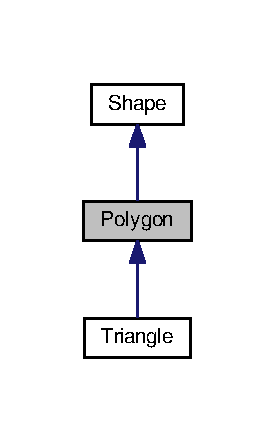
\includegraphics[width=132pt]{class_polygon__inherit__graph}
\end{center}
\end{figure}


Collaboration diagram for Polygon\+:\nopagebreak
\begin{figure}[H]
\begin{center}
\leavevmode
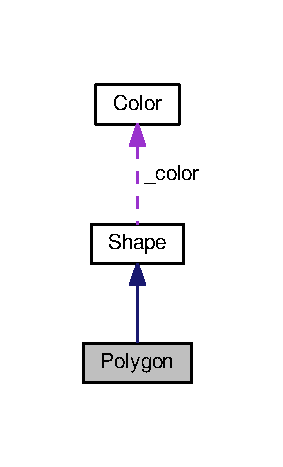
\includegraphics[width=136pt]{class_polygon__coll__graph}
\end{center}
\end{figure}
\subsection*{Public Member Functions}
\begin{DoxyCompactItemize}
\item 
\hyperlink{class_polygon_a9010c30fc3b029a2cc26199c15f915b6}{Polygon} (const \hyperlink{class_color}{Color} \&color=\hyperlink{class_color_a94697e8c9eb81124c5a7c1439e1e7348}{Color\+::get\+Color}(\char`\"{}black\char`\"{}))
\item 
void \hyperlink{class_polygon_a9a5b91783fca1fd154bc97a1e416500b}{add\+Point} (const \hyperlink{class_vector2_d}{Vector2D} \&point)
\item 
const \hyperlink{class_vector2_d}{Vector2D} \hyperlink{class_polygon_ae488fc076f6a3ca6b36ae6217b38195d}{get\+Point} (int index) const
\item 
const int \hyperlink{class_polygon_a07f0c79bf97308da04c7bce322331cab}{get\+Points\+Size} () const
\item 
void \hyperlink{class_polygon_a245c526a6a65ea99f5549fe5243006d0}{draw} (\hyperlink{class_drawing_visitor}{Drawing\+Visitor} $\ast$visitor) const
\item 
\hyperlink{class_polygon_a41c29b75f2463646af0f7bd604a4853d}{operator string} () const
\item 
void \hyperlink{class_polygon_ad9adb867821b71e1aa8130dccbc9b37f}{save} (const \hyperlink{class_save_visitor}{Save\+Visitor} $\ast$save\+Visitor, const string \&filename) const
\item 
\hyperlink{class_shape}{Shape} $\ast$ \hyperlink{class_polygon_ae828addfa5cffab547bcb16db1f275be}{translation} (const \hyperlink{class_vector2_d}{Vector2D} \&translation\+Vector) const
\item 
\hyperlink{class_shape}{Shape} $\ast$ \hyperlink{class_polygon_a2b77c7ecbe9ca68664d7f7020181b791}{homothety} (const \hyperlink{class_vector2_d}{Vector2D} \&invariant\+Point, const double \&homothety\+Ratio) const
\item 
\hyperlink{class_shape}{Shape} $\ast$ \hyperlink{class_polygon_a5a453f01700f97ca98b0487cd670b194}{rotation} (const \hyperlink{class_vector2_d}{Vector2D} \&rotation\+Center, const \hyperlink{class_radian_angle}{Radian\+Angle} \&rotation\+Angle) const
\item 
double \hyperlink{class_polygon_ae1ae9dd5e5613f119af3e31488427b01}{get\+Area} () const
\end{DoxyCompactItemize}
\subsection*{Protected Attributes}
\begin{DoxyCompactItemize}
\item 
std\+::vector$<$ \hyperlink{class_vector2_d}{Vector2D} $>$ \hyperlink{class_polygon_a36bc7384f59aac1a731f1701af587916}{\+\_\+points}
\end{DoxyCompactItemize}
\subsection*{Friends}
\begin{DoxyCompactItemize}
\item 
ostream \& \hyperlink{class_polygon_af7ce19139e0c1e3637615abf41b8befb}{operator$<$$<$} (ostream \&os, const \hyperlink{class_polygon}{Polygon} \&polygon)
\end{DoxyCompactItemize}


\subsection{Detailed Description}
Represent a \hyperlink{class_polygon}{Polygon} It\textquotesingle{}s a \hyperlink{class_shape}{Shape} 

\subsection{Constructor \& Destructor Documentation}
\hypertarget{class_polygon_a9010c30fc3b029a2cc26199c15f915b6}{}\label{class_polygon_a9010c30fc3b029a2cc26199c15f915b6} 
\index{Polygon@{Polygon}!Polygon@{Polygon}}
\index{Polygon@{Polygon}!Polygon@{Polygon}}
\subsubsection{\texorpdfstring{Polygon()}{Polygon()}}
{\footnotesize\ttfamily Polygon\+::\+Polygon (\begin{DoxyParamCaption}\item[{const \hyperlink{class_color}{Color} \&}]{color = {\ttfamily \hyperlink{class_color_a94697e8c9eb81124c5a7c1439e1e7348}{Color\+::get\+Color}(\char`\"{}black\char`\"{})} }\end{DoxyParamCaption})}

\hyperlink{class_polygon}{Polygon} constructor 
\begin{DoxyParams}{Parameters}
{\em color} & the color of the \hyperlink{class_polygon}{Polygon} \\
\hline
\end{DoxyParams}


\subsection{Member Function Documentation}
\hypertarget{class_polygon_a9a5b91783fca1fd154bc97a1e416500b}{}\label{class_polygon_a9a5b91783fca1fd154bc97a1e416500b} 
\index{Polygon@{Polygon}!add\+Point@{add\+Point}}
\index{add\+Point@{add\+Point}!Polygon@{Polygon}}
\subsubsection{\texorpdfstring{add\+Point()}{addPoint()}}
{\footnotesize\ttfamily void Polygon\+::add\+Point (\begin{DoxyParamCaption}\item[{const \hyperlink{class_vector2_d}{Vector2D} \&}]{point }\end{DoxyParamCaption})}

Function to add a point on the \hyperlink{class_polygon}{Polygon} 
\begin{DoxyParams}{Parameters}
{\em point} & point to add \\
\hline
\end{DoxyParams}
\hypertarget{class_polygon_a245c526a6a65ea99f5549fe5243006d0}{}\label{class_polygon_a245c526a6a65ea99f5549fe5243006d0} 
\index{Polygon@{Polygon}!draw@{draw}}
\index{draw@{draw}!Polygon@{Polygon}}
\subsubsection{\texorpdfstring{draw()}{draw()}}
{\footnotesize\ttfamily void Polygon\+::draw (\begin{DoxyParamCaption}\item[{\hyperlink{class_drawing_visitor}{Drawing\+Visitor} $\ast$}]{visitor }\end{DoxyParamCaption}) const\hspace{0.3cm}{\ttfamily [virtual]}}

Draws the \hyperlink{class_polygon}{Polygon} using a \hyperlink{class_drawing_visitor}{Drawing\+Visitor}. 
\begin{DoxyParams}{Parameters}
{\em visitor} & The \hyperlink{class_drawing_visitor}{Drawing\+Visitor} to use to draw the \hyperlink{class_polygon}{Polygon}. \\
\hline
\end{DoxyParams}


Implements \hyperlink{class_shape_ae67fc6d39dd33759b65ff6112b21eab7}{Shape}.



Reimplemented in \hyperlink{class_triangle_a1fa834143ed718605959a227eba573b3}{Triangle}.

\hypertarget{class_polygon_ae1ae9dd5e5613f119af3e31488427b01}{}\label{class_polygon_ae1ae9dd5e5613f119af3e31488427b01} 
\index{Polygon@{Polygon}!get\+Area@{get\+Area}}
\index{get\+Area@{get\+Area}!Polygon@{Polygon}}
\subsubsection{\texorpdfstring{get\+Area()}{getArea()}}
{\footnotesize\ttfamily double Polygon\+::get\+Area (\begin{DoxyParamCaption}{ }\end{DoxyParamCaption}) const\hspace{0.3cm}{\ttfamily [virtual]}}

Returns the area of the \hyperlink{class_polygon}{Polygon}. \begin{DoxyReturn}{Returns}
The area of the \hyperlink{class_polygon}{Polygon}. 
\end{DoxyReturn}


Implements \hyperlink{class_shape_ad9454ee04617290547e7529180b1beae}{Shape}.



Reimplemented in \hyperlink{class_triangle_a5f7fa9fd678345063e50e3458d943a9b}{Triangle}.

\hypertarget{class_polygon_ae488fc076f6a3ca6b36ae6217b38195d}{}\label{class_polygon_ae488fc076f6a3ca6b36ae6217b38195d} 
\index{Polygon@{Polygon}!get\+Point@{get\+Point}}
\index{get\+Point@{get\+Point}!Polygon@{Polygon}}
\subsubsection{\texorpdfstring{get\+Point()}{getPoint()}}
{\footnotesize\ttfamily const \hyperlink{class_vector2_d}{Vector2D} Polygon\+::get\+Point (\begin{DoxyParamCaption}\item[{int}]{index }\end{DoxyParamCaption}) const}

Function to get a point of \+\_\+points with index  index the index of point to get \begin{DoxyReturn}{Returns}
\hyperlink{class_vector2_d}{Vector2D} the point 
\end{DoxyReturn}
\hypertarget{class_polygon_a07f0c79bf97308da04c7bce322331cab}{}\label{class_polygon_a07f0c79bf97308da04c7bce322331cab} 
\index{Polygon@{Polygon}!get\+Points\+Size@{get\+Points\+Size}}
\index{get\+Points\+Size@{get\+Points\+Size}!Polygon@{Polygon}}
\subsubsection{\texorpdfstring{get\+Points\+Size()}{getPointsSize()}}
{\footnotesize\ttfamily const int Polygon\+::get\+Points\+Size (\begin{DoxyParamCaption}{ }\end{DoxyParamCaption}) const}

Function to get the size of \+\_\+points \begin{DoxyReturn}{Returns}
int the size of \+\_\+points 
\end{DoxyReturn}
\hypertarget{class_polygon_a2b77c7ecbe9ca68664d7f7020181b791}{}\label{class_polygon_a2b77c7ecbe9ca68664d7f7020181b791} 
\index{Polygon@{Polygon}!homothety@{homothety}}
\index{homothety@{homothety}!Polygon@{Polygon}}
\subsubsection{\texorpdfstring{homothety()}{homothety()}}
{\footnotesize\ttfamily \hyperlink{class_shape}{Shape} $\ast$ Polygon\+::homothety (\begin{DoxyParamCaption}\item[{const \hyperlink{class_vector2_d}{Vector2D} \&}]{invariant\+Point,  }\item[{const double \&}]{homothety\+Ratio }\end{DoxyParamCaption}) const\hspace{0.3cm}{\ttfamily [virtual]}}

Apply an homothety on the \hyperlink{class_polygon}{Polygon}. 
\begin{DoxyParams}{Parameters}
{\em invariant\+Point} & The center of the homothety. \\
\hline
{\em homothety\+Ratio} & The ratio of the homothety. \\
\hline
\end{DoxyParams}
\begin{DoxyReturn}{Returns}
Shape$\ast$ the new \hyperlink{class_polygon}{Polygon} after homothety 
\end{DoxyReturn}


Implements \hyperlink{class_shape_a91f18af3004ba210db5c91084c50beb9}{Shape}.



Reimplemented in \hyperlink{class_triangle_a45a3a9f74118c99b95c6d8e993773a71}{Triangle}.

\hypertarget{class_polygon_a41c29b75f2463646af0f7bd604a4853d}{}\label{class_polygon_a41c29b75f2463646af0f7bd604a4853d} 
\index{Polygon@{Polygon}!operator string@{operator string}}
\index{operator string@{operator string}!Polygon@{Polygon}}
\subsubsection{\texorpdfstring{operator string()}{operator string()}}
{\footnotesize\ttfamily Polygon\+::operator string (\begin{DoxyParamCaption}{ }\end{DoxyParamCaption}) const\hspace{0.3cm}{\ttfamily [virtual]}}

Returns a string that represents the \hyperlink{class_polygon}{Polygon}. \begin{DoxyReturn}{Returns}
The string representing the \hyperlink{class_polygon}{Polygon}. 
\end{DoxyReturn}


Implements \hyperlink{class_shape_a0d74dcb2db0791b88b92f439bf4a6972}{Shape}.



Reimplemented in \hyperlink{class_triangle_acd8612cc20ffb71e543944c869e4ab81}{Triangle}.

\hypertarget{class_polygon_a5a453f01700f97ca98b0487cd670b194}{}\label{class_polygon_a5a453f01700f97ca98b0487cd670b194} 
\index{Polygon@{Polygon}!rotation@{rotation}}
\index{rotation@{rotation}!Polygon@{Polygon}}
\subsubsection{\texorpdfstring{rotation()}{rotation()}}
{\footnotesize\ttfamily \hyperlink{class_shape}{Shape} $\ast$ Polygon\+::rotation (\begin{DoxyParamCaption}\item[{const \hyperlink{class_vector2_d}{Vector2D} \&}]{rotation\+Center,  }\item[{const \hyperlink{class_radian_angle}{Radian\+Angle} \&}]{rotation\+Angle }\end{DoxyParamCaption}) const\hspace{0.3cm}{\ttfamily [virtual]}}

Rotates the \hyperlink{class_polygon}{Polygon}. 
\begin{DoxyParams}{Parameters}
{\em rotation\+Center} & The center of the rotation. \\
\hline
{\em rotation\+Angle} & The angle of the rotation. \\
\hline
\end{DoxyParams}
\begin{DoxyReturn}{Returns}
Shape$\ast$ the new \hyperlink{class_polygon}{Polygon} after rotation 
\end{DoxyReturn}


Implements \hyperlink{class_shape_abfc7a673b8a6d9a4d646dc15c771aa0d}{Shape}.



Reimplemented in \hyperlink{class_triangle_a663ca3c6bd7967265849bf1f8c8a464b}{Triangle}.

\hypertarget{class_polygon_ad9adb867821b71e1aa8130dccbc9b37f}{}\label{class_polygon_ad9adb867821b71e1aa8130dccbc9b37f} 
\index{Polygon@{Polygon}!save@{save}}
\index{save@{save}!Polygon@{Polygon}}
\subsubsection{\texorpdfstring{save()}{save()}}
{\footnotesize\ttfamily void Polygon\+::save (\begin{DoxyParamCaption}\item[{const \hyperlink{class_save_visitor}{Save\+Visitor} $\ast$}]{save\+Visitor,  }\item[{const string \&}]{filename }\end{DoxyParamCaption}) const\hspace{0.3cm}{\ttfamily [virtual]}}

Saves the \hyperlink{class_polygon}{Polygon}. 
\begin{DoxyParams}{Parameters}
{\em save\+Visitor} & The \hyperlink{class_save_visitor}{Save\+Visitor} to use to save the \hyperlink{class_polygon}{Polygon}. \\
\hline
\end{DoxyParams}


Implements \hyperlink{class_shape_ae1477829e1b06aad805b8b76312f87bc}{Shape}.



Reimplemented in \hyperlink{class_triangle_ae9ac3d633172f14d391d290a4467e1d3}{Triangle}.

\hypertarget{class_polygon_ae828addfa5cffab547bcb16db1f275be}{}\label{class_polygon_ae828addfa5cffab547bcb16db1f275be} 
\index{Polygon@{Polygon}!translation@{translation}}
\index{translation@{translation}!Polygon@{Polygon}}
\subsubsection{\texorpdfstring{translation()}{translation()}}
{\footnotesize\ttfamily \hyperlink{class_shape}{Shape} $\ast$ Polygon\+::translation (\begin{DoxyParamCaption}\item[{const \hyperlink{class_vector2_d}{Vector2D} \&}]{translation\+Vector }\end{DoxyParamCaption}) const\hspace{0.3cm}{\ttfamily [virtual]}}

Translate the \hyperlink{class_polygon}{Polygon} using a translation vector. 
\begin{DoxyParams}{Parameters}
{\em translation\+Vector} & The translation vector to use for the translation. \\
\hline
\end{DoxyParams}
\begin{DoxyReturn}{Returns}
Shape$\ast$ the new \hyperlink{class_polygon}{Polygon} after Translation 
\end{DoxyReturn}


Implements \hyperlink{class_shape_ad3daca0d9bedf9aa15b92afab63c1de8}{Shape}.



Reimplemented in \hyperlink{class_triangle_ac66208b0b633add41b915860f051cf44}{Triangle}.



\subsection{Friends And Related Function Documentation}
\hypertarget{class_polygon_af7ce19139e0c1e3637615abf41b8befb}{}\label{class_polygon_af7ce19139e0c1e3637615abf41b8befb} 
\index{Polygon@{Polygon}!operator$<$$<$@{operator$<$$<$}}
\index{operator$<$$<$@{operator$<$$<$}!Polygon@{Polygon}}
\subsubsection{\texorpdfstring{operator$<$$<$}{operator<<}}
{\footnotesize\ttfamily ostream\& operator$<$$<$ (\begin{DoxyParamCaption}\item[{ostream \&}]{os,  }\item[{const \hyperlink{class_polygon}{Polygon} \&}]{polygon }\end{DoxyParamCaption})\hspace{0.3cm}{\ttfamily [friend]}}



\subsection{Member Data Documentation}
\hypertarget{class_polygon_a36bc7384f59aac1a731f1701af587916}{}\label{class_polygon_a36bc7384f59aac1a731f1701af587916} 
\index{Polygon@{Polygon}!\+\_\+points@{\+\_\+points}}
\index{\+\_\+points@{\+\_\+points}!Polygon@{Polygon}}
\subsubsection{\texorpdfstring{\+\_\+points}{\_points}}
{\footnotesize\ttfamily std\+::vector$<$\hyperlink{class_vector2_d}{Vector2D}$>$ Polygon\+::\+\_\+points\hspace{0.3cm}{\ttfamily [protected]}}

Array of \hyperlink{class_vector2_d}{Vector2D} for store points of the \hyperlink{class_polygon}{Polygon} 

The documentation for this class was generated from the following files\+:\begin{DoxyCompactItemize}
\item 
src/\+Shape/\hyperlink{_polygon_8hpp}{Polygon.\+hpp}\item 
src/\+Shape/\hyperlink{_polygon_8cpp}{Polygon.\+cpp}\end{DoxyCompactItemize}

\hypertarget{class_polygon_creator}{}\section{Polygon\+Creator Class Reference}
\label{class_polygon_creator}\index{Polygon\+Creator@{Polygon\+Creator}}


{\ttfamily \#include $<$Polygon\+Creator.\+hpp$>$}



Inheritance diagram for Polygon\+Creator\+:\nopagebreak
\begin{figure}[H]
\begin{center}
\leavevmode
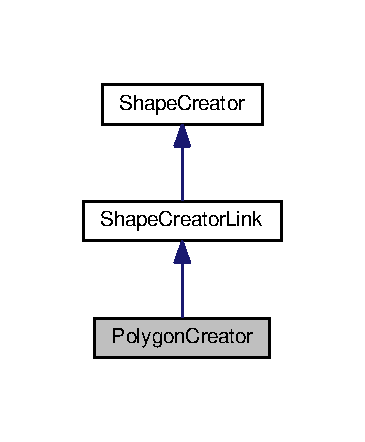
\includegraphics[width=175pt]{class_polygon_creator__inherit__graph}
\end{center}
\end{figure}


Collaboration diagram for Polygon\+Creator\+:\nopagebreak
\begin{figure}[H]
\begin{center}
\leavevmode
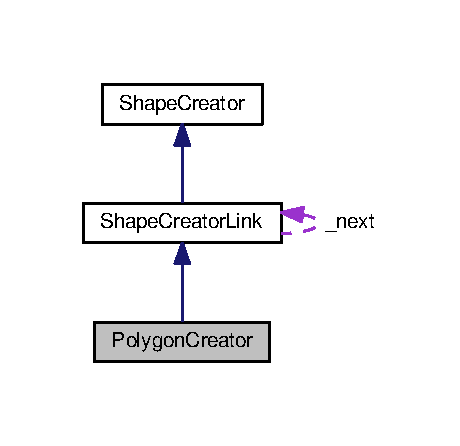
\includegraphics[width=221pt]{class_polygon_creator__coll__graph}
\end{center}
\end{figure}
\subsection*{Public Member Functions}
\begin{DoxyCompactItemize}
\item 
\hyperlink{class_polygon_creator_ab0d3a2c045b483938bda8cffc6173e42}{Polygon\+Creator} (\hyperlink{class_shape_creator_link}{Shape\+Creator\+Link} $\ast$next)
\item 
virtual \hyperlink{class_shape}{Shape} $\ast$ \hyperlink{class_polygon_creator_ad7a34580d4291a50fe189c912c7b32a0}{create\+Shape\+Spe} (const string \&shape\+String) const
\end{DoxyCompactItemize}
\subsection*{Additional Inherited Members}


\subsection{Detailed Description}
Class \hyperlink{class_polygon_creator}{Polygon\+Creator} Link of the C\+OR for build \hyperlink{class_polygon}{Polygon} 

\subsection{Constructor \& Destructor Documentation}
\hypertarget{class_polygon_creator_ab0d3a2c045b483938bda8cffc6173e42}{}\label{class_polygon_creator_ab0d3a2c045b483938bda8cffc6173e42} 
\index{Polygon\+Creator@{Polygon\+Creator}!Polygon\+Creator@{Polygon\+Creator}}
\index{Polygon\+Creator@{Polygon\+Creator}!Polygon\+Creator@{Polygon\+Creator}}
\subsubsection{\texorpdfstring{Polygon\+Creator()}{PolygonCreator()}}
{\footnotesize\ttfamily Polygon\+Creator\+::\+Polygon\+Creator (\begin{DoxyParamCaption}\item[{\hyperlink{class_shape_creator_link}{Shape\+Creator\+Link} $\ast$}]{next }\end{DoxyParamCaption})}

Constructor of \hyperlink{class_polygon_creator}{Polygon\+Creator} 
\begin{DoxyParams}{Parameters}
{\em next} & The next \hyperlink{class_shape_creator_link}{Shape\+Creator\+Link} if this one fails \\
\hline
\end{DoxyParams}


\subsection{Member Function Documentation}
\hypertarget{class_polygon_creator_ad7a34580d4291a50fe189c912c7b32a0}{}\label{class_polygon_creator_ad7a34580d4291a50fe189c912c7b32a0} 
\index{Polygon\+Creator@{Polygon\+Creator}!create\+Shape\+Spe@{create\+Shape\+Spe}}
\index{create\+Shape\+Spe@{create\+Shape\+Spe}!Polygon\+Creator@{Polygon\+Creator}}
\subsubsection{\texorpdfstring{create\+Shape\+Spe()}{createShapeSpe()}}
{\footnotesize\ttfamily \hyperlink{class_shape}{Shape} $\ast$ Polygon\+Creator\+::create\+Shape\+Spe (\begin{DoxyParamCaption}\item[{const string \&}]{shape\+String }\end{DoxyParamCaption}) const\hspace{0.3cm}{\ttfamily [virtual]}}

Try to create a \hyperlink{class_polygon}{Polygon} with the string 
\begin{DoxyParams}{Parameters}
{\em shape\+String} & the string with informations of the shape \\
\hline
\end{DoxyParams}
\begin{DoxyReturn}{Returns}
The Shape$\ast$ wich were created 
\end{DoxyReturn}


Implements \hyperlink{class_shape_creator_link_a036ecc845946d23b36335e9077308bcf}{Shape\+Creator\+Link}.



The documentation for this class was generated from the following files\+:\begin{DoxyCompactItemize}
\item 
src/\+Loader/\hyperlink{_polygon_creator_8hpp}{Polygon\+Creator.\+hpp}\item 
src/\+Loader/\hyperlink{_polygon_creator_8cpp}{Polygon\+Creator.\+cpp}\end{DoxyCompactItemize}

\hypertarget{class_qt_drawer}{}\section{Qt\+Drawer Class Reference}
\label{class_qt_drawer}\index{Qt\+Drawer@{Qt\+Drawer}}


{\ttfamily \#include $<$Qt\+Drawer.\+hpp$>$}



Inheritance diagram for Qt\+Drawer\+:\nopagebreak
\begin{figure}[H]
\begin{center}
\leavevmode
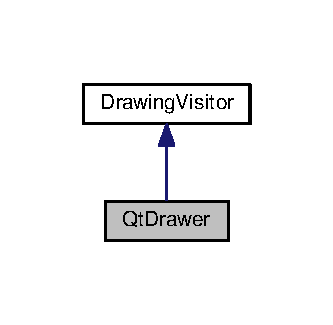
\includegraphics[width=160pt]{class_qt_drawer__inherit__graph}
\end{center}
\end{figure}


Collaboration diagram for Qt\+Drawer\+:\nopagebreak
\begin{figure}[H]
\begin{center}
\leavevmode
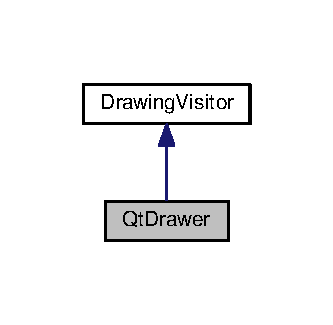
\includegraphics[width=160pt]{class_qt_drawer__coll__graph}
\end{center}
\end{figure}
\subsection*{Public Member Functions}
\begin{DoxyCompactItemize}
\item 
\hyperlink{class_qt_drawer_a1d7dce4e986de57aa3dfb7f39052b54e}{Qt\+Drawer} ()
\item 
virtual \hyperlink{class_qt_drawer_a73b63daa39c4824da08c1486b099a160}{$\sim$\+Qt\+Drawer} ()
\item 
void \hyperlink{class_qt_drawer_a1e9a6ad76355f26fc9b41b54b28a04f4}{draw} (const \hyperlink{class_circle}{Circle} $\ast$circle)
\item 
void \hyperlink{class_qt_drawer_afe2f299e83092e1d4676c8b3fd4a3452}{draw} (const \hyperlink{class_segment}{Segment} $\ast$segment)
\item 
void \hyperlink{class_qt_drawer_a6d68080c84447a76b34810ca0330fd2c}{draw} (const \hyperlink{class_triangle}{Triangle} $\ast$triangle)
\item 
void \hyperlink{class_qt_drawer_a977cc5f97827eb36063f8429ef044727}{draw} (const \hyperlink{class_polygon}{Polygon} $\ast$polygon)
\item 
void \hyperlink{class_qt_drawer_a031e3b3242e341fa6e6fdcbf96b3dbfe}{draw} (const \hyperlink{class_shape}{Shape} $\ast$shape)
\item 
void \hyperlink{class_qt_drawer_a404a989a5cf6f7b5e7469e251045dacb}{add\+To\+Scene} (const \hyperlink{class_circle}{Circle} $\ast$circle)
\item 
void \hyperlink{class_qt_drawer_a7210a0775cf19ce5de0601028c8d7712}{add\+To\+Scene} (const \hyperlink{class_segment}{Segment} $\ast$segment)
\item 
void \hyperlink{class_qt_drawer_a5515539c77eb172644859e115a8044bc}{add\+To\+Scene} (const \hyperlink{class_triangle}{Triangle} $\ast$triangle)
\item 
void \hyperlink{class_qt_drawer_a48a8a31ffdc14e6122b78779c0cdfb39}{add\+To\+Scene} (const \hyperlink{class_polygon}{Polygon} $\ast$polygon)
\item 
void \hyperlink{class_qt_drawer_adaec0c490edc2cd18ece227a0f56dbfa}{add\+To\+Scene} (const \hyperlink{class_composed_shape}{Composed\+Shape} $\ast$composed\+Shape)
\item 
void \hyperlink{class_qt_drawer_a43c474754631c15519485533caf18a89}{display\+Window} ()
\end{DoxyCompactItemize}


\subsection{Detailed Description}
This class is the drawer that implement a way to draw shapes using Qt 

\subsection{Constructor \& Destructor Documentation}
\hypertarget{class_qt_drawer_a1d7dce4e986de57aa3dfb7f39052b54e}{}\label{class_qt_drawer_a1d7dce4e986de57aa3dfb7f39052b54e} 
\index{Qt\+Drawer@{Qt\+Drawer}!Qt\+Drawer@{Qt\+Drawer}}
\index{Qt\+Drawer@{Qt\+Drawer}!Qt\+Drawer@{Qt\+Drawer}}
\subsubsection{\texorpdfstring{Qt\+Drawer()}{QtDrawer()}}
{\footnotesize\ttfamily Qt\+Drawer\+::\+Qt\+Drawer (\begin{DoxyParamCaption}{ }\end{DoxyParamCaption})}

\hypertarget{class_qt_drawer_a73b63daa39c4824da08c1486b099a160}{}\label{class_qt_drawer_a73b63daa39c4824da08c1486b099a160} 
\index{Qt\+Drawer@{Qt\+Drawer}!````~Qt\+Drawer@{$\sim$\+Qt\+Drawer}}
\index{````~Qt\+Drawer@{$\sim$\+Qt\+Drawer}!Qt\+Drawer@{Qt\+Drawer}}
\subsubsection{\texorpdfstring{$\sim$\+Qt\+Drawer()}{~QtDrawer()}}
{\footnotesize\ttfamily Qt\+Drawer\+::$\sim$\+Qt\+Drawer (\begin{DoxyParamCaption}{ }\end{DoxyParamCaption})\hspace{0.3cm}{\ttfamily [virtual]}}



\subsection{Member Function Documentation}
\hypertarget{class_qt_drawer_a404a989a5cf6f7b5e7469e251045dacb}{}\label{class_qt_drawer_a404a989a5cf6f7b5e7469e251045dacb} 
\index{Qt\+Drawer@{Qt\+Drawer}!add\+To\+Scene@{add\+To\+Scene}}
\index{add\+To\+Scene@{add\+To\+Scene}!Qt\+Drawer@{Qt\+Drawer}}
\subsubsection{\texorpdfstring{add\+To\+Scene()}{addToScene()}\hspace{0.1cm}{\footnotesize\ttfamily [1/5]}}
{\footnotesize\ttfamily void Qt\+Drawer\+::add\+To\+Scene (\begin{DoxyParamCaption}\item[{const \hyperlink{class_circle}{Circle} $\ast$}]{circle }\end{DoxyParamCaption})}

Add the \hyperlink{class_circle}{Circle} to the scene. 
\begin{DoxyParams}{Parameters}
{\em circle} & The \hyperlink{class_circle}{Circle} to add to the scene. \\
\hline
\end{DoxyParams}
\hypertarget{class_qt_drawer_a7210a0775cf19ce5de0601028c8d7712}{}\label{class_qt_drawer_a7210a0775cf19ce5de0601028c8d7712} 
\index{Qt\+Drawer@{Qt\+Drawer}!add\+To\+Scene@{add\+To\+Scene}}
\index{add\+To\+Scene@{add\+To\+Scene}!Qt\+Drawer@{Qt\+Drawer}}
\subsubsection{\texorpdfstring{add\+To\+Scene()}{addToScene()}\hspace{0.1cm}{\footnotesize\ttfamily [2/5]}}
{\footnotesize\ttfamily void Qt\+Drawer\+::add\+To\+Scene (\begin{DoxyParamCaption}\item[{const \hyperlink{class_segment}{Segment} $\ast$}]{segment }\end{DoxyParamCaption})}

Add the \hyperlink{class_segment}{Segment} to the scene. 
\begin{DoxyParams}{Parameters}
{\em segment} & The \hyperlink{class_segment}{Segment} to add to the scene. \\
\hline
\end{DoxyParams}
\hypertarget{class_qt_drawer_a5515539c77eb172644859e115a8044bc}{}\label{class_qt_drawer_a5515539c77eb172644859e115a8044bc} 
\index{Qt\+Drawer@{Qt\+Drawer}!add\+To\+Scene@{add\+To\+Scene}}
\index{add\+To\+Scene@{add\+To\+Scene}!Qt\+Drawer@{Qt\+Drawer}}
\subsubsection{\texorpdfstring{add\+To\+Scene()}{addToScene()}\hspace{0.1cm}{\footnotesize\ttfamily [3/5]}}
{\footnotesize\ttfamily void Qt\+Drawer\+::add\+To\+Scene (\begin{DoxyParamCaption}\item[{const \hyperlink{class_triangle}{Triangle} $\ast$}]{triangle }\end{DoxyParamCaption})}

Add the \hyperlink{class_triangle}{Triangle} to the scene. 
\begin{DoxyParams}{Parameters}
{\em triangle} & The \hyperlink{class_triangle}{Triangle} to add to the scene. \\
\hline
\end{DoxyParams}
\hypertarget{class_qt_drawer_a48a8a31ffdc14e6122b78779c0cdfb39}{}\label{class_qt_drawer_a48a8a31ffdc14e6122b78779c0cdfb39} 
\index{Qt\+Drawer@{Qt\+Drawer}!add\+To\+Scene@{add\+To\+Scene}}
\index{add\+To\+Scene@{add\+To\+Scene}!Qt\+Drawer@{Qt\+Drawer}}
\subsubsection{\texorpdfstring{add\+To\+Scene()}{addToScene()}\hspace{0.1cm}{\footnotesize\ttfamily [4/5]}}
{\footnotesize\ttfamily void Qt\+Drawer\+::add\+To\+Scene (\begin{DoxyParamCaption}\item[{const \hyperlink{class_polygon}{Polygon} $\ast$}]{polygon }\end{DoxyParamCaption})}

Add the \hyperlink{class_polygon}{Polygon} to the scene. 
\begin{DoxyParams}{Parameters}
{\em polygon} & The \hyperlink{class_polygon}{Polygon} to add to the scene. \\
\hline
\end{DoxyParams}
\hypertarget{class_qt_drawer_adaec0c490edc2cd18ece227a0f56dbfa}{}\label{class_qt_drawer_adaec0c490edc2cd18ece227a0f56dbfa} 
\index{Qt\+Drawer@{Qt\+Drawer}!add\+To\+Scene@{add\+To\+Scene}}
\index{add\+To\+Scene@{add\+To\+Scene}!Qt\+Drawer@{Qt\+Drawer}}
\subsubsection{\texorpdfstring{add\+To\+Scene()}{addToScene()}\hspace{0.1cm}{\footnotesize\ttfamily [5/5]}}
{\footnotesize\ttfamily void Qt\+Drawer\+::add\+To\+Scene (\begin{DoxyParamCaption}\item[{const \hyperlink{class_composed_shape}{Composed\+Shape} $\ast$}]{composed\+Shape }\end{DoxyParamCaption})}

Add the \hyperlink{class_composed_shape}{Composed\+Shape} to the scene. 
\begin{DoxyParams}{Parameters}
{\em composed\+Shape} & The \hyperlink{class_composed_shape}{Composed\+Shape} to add to the scene. \\
\hline
\end{DoxyParams}
\hypertarget{class_qt_drawer_a43c474754631c15519485533caf18a89}{}\label{class_qt_drawer_a43c474754631c15519485533caf18a89} 
\index{Qt\+Drawer@{Qt\+Drawer}!display\+Window@{display\+Window}}
\index{display\+Window@{display\+Window}!Qt\+Drawer@{Qt\+Drawer}}
\subsubsection{\texorpdfstring{display\+Window()}{displayWindow()}}
{\footnotesize\ttfamily void Qt\+Drawer\+::display\+Window (\begin{DoxyParamCaption}{ }\end{DoxyParamCaption})}

Sets the scene to the view and display it. \hypertarget{class_qt_drawer_a1e9a6ad76355f26fc9b41b54b28a04f4}{}\label{class_qt_drawer_a1e9a6ad76355f26fc9b41b54b28a04f4} 
\index{Qt\+Drawer@{Qt\+Drawer}!draw@{draw}}
\index{draw@{draw}!Qt\+Drawer@{Qt\+Drawer}}
\subsubsection{\texorpdfstring{draw()}{draw()}\hspace{0.1cm}{\footnotesize\ttfamily [1/5]}}
{\footnotesize\ttfamily void Qt\+Drawer\+::draw (\begin{DoxyParamCaption}\item[{const \hyperlink{class_circle}{Circle} $\ast$}]{circle }\end{DoxyParamCaption})\hspace{0.3cm}{\ttfamily [virtual]}}

Draws the \hyperlink{class_circle}{Circle}. 
\begin{DoxyParams}{Parameters}
{\em circle} & The \hyperlink{class_circle}{Circle} to draw. \\
\hline
\end{DoxyParams}


Implements \hyperlink{class_drawing_visitor_a287f6d770c755c1c3bc144fb08b65030}{Drawing\+Visitor}.

\hypertarget{class_qt_drawer_afe2f299e83092e1d4676c8b3fd4a3452}{}\label{class_qt_drawer_afe2f299e83092e1d4676c8b3fd4a3452} 
\index{Qt\+Drawer@{Qt\+Drawer}!draw@{draw}}
\index{draw@{draw}!Qt\+Drawer@{Qt\+Drawer}}
\subsubsection{\texorpdfstring{draw()}{draw()}\hspace{0.1cm}{\footnotesize\ttfamily [2/5]}}
{\footnotesize\ttfamily void Qt\+Drawer\+::draw (\begin{DoxyParamCaption}\item[{const \hyperlink{class_segment}{Segment} $\ast$}]{segment }\end{DoxyParamCaption})\hspace{0.3cm}{\ttfamily [virtual]}}

Draws the \hyperlink{class_segment}{Segment}. 
\begin{DoxyParams}{Parameters}
{\em segment} & The \hyperlink{class_segment}{Segment} to draw. \\
\hline
\end{DoxyParams}


Implements \hyperlink{class_drawing_visitor_a8a95018de31a7e3d7a067c347478ffde}{Drawing\+Visitor}.

\hypertarget{class_qt_drawer_a6d68080c84447a76b34810ca0330fd2c}{}\label{class_qt_drawer_a6d68080c84447a76b34810ca0330fd2c} 
\index{Qt\+Drawer@{Qt\+Drawer}!draw@{draw}}
\index{draw@{draw}!Qt\+Drawer@{Qt\+Drawer}}
\subsubsection{\texorpdfstring{draw()}{draw()}\hspace{0.1cm}{\footnotesize\ttfamily [3/5]}}
{\footnotesize\ttfamily void Qt\+Drawer\+::draw (\begin{DoxyParamCaption}\item[{const \hyperlink{class_triangle}{Triangle} $\ast$}]{triangle }\end{DoxyParamCaption})\hspace{0.3cm}{\ttfamily [virtual]}}

Draws the \hyperlink{class_triangle}{Triangle}. 
\begin{DoxyParams}{Parameters}
{\em triangle} & The \hyperlink{class_triangle}{Triangle} to draw. \\
\hline
\end{DoxyParams}


Implements \hyperlink{class_drawing_visitor_a178aa7e1bb9cfbd538d7de0dbfa2d4b1}{Drawing\+Visitor}.

\hypertarget{class_qt_drawer_a977cc5f97827eb36063f8429ef044727}{}\label{class_qt_drawer_a977cc5f97827eb36063f8429ef044727} 
\index{Qt\+Drawer@{Qt\+Drawer}!draw@{draw}}
\index{draw@{draw}!Qt\+Drawer@{Qt\+Drawer}}
\subsubsection{\texorpdfstring{draw()}{draw()}\hspace{0.1cm}{\footnotesize\ttfamily [4/5]}}
{\footnotesize\ttfamily void Qt\+Drawer\+::draw (\begin{DoxyParamCaption}\item[{const \hyperlink{class_polygon}{Polygon} $\ast$}]{polygon }\end{DoxyParamCaption})\hspace{0.3cm}{\ttfamily [virtual]}}

Draws the \hyperlink{class_polygon}{Polygon}. 
\begin{DoxyParams}{Parameters}
{\em polygon} & The \hyperlink{class_polygon}{Polygon} to draw. \\
\hline
\end{DoxyParams}


Implements \hyperlink{class_drawing_visitor_a771a2110a3afe4e87688bddd65657a46}{Drawing\+Visitor}.

\hypertarget{class_qt_drawer_a031e3b3242e341fa6e6fdcbf96b3dbfe}{}\label{class_qt_drawer_a031e3b3242e341fa6e6fdcbf96b3dbfe} 
\index{Qt\+Drawer@{Qt\+Drawer}!draw@{draw}}
\index{draw@{draw}!Qt\+Drawer@{Qt\+Drawer}}
\subsubsection{\texorpdfstring{draw()}{draw()}\hspace{0.1cm}{\footnotesize\ttfamily [5/5]}}
{\footnotesize\ttfamily void Qt\+Drawer\+::draw (\begin{DoxyParamCaption}\item[{const \hyperlink{class_shape}{Shape} $\ast$}]{shape }\end{DoxyParamCaption})\hspace{0.3cm}{\ttfamily [virtual]}}

Draws the \hyperlink{class_shape}{Shape}. 
\begin{DoxyParams}{Parameters}
{\em shape} & The \hyperlink{class_shape}{Shape} to draw. \\
\hline
\end{DoxyParams}


Implements \hyperlink{class_drawing_visitor_ad3d9e3028449f65ea2c405c74c4a55b4}{Drawing\+Visitor}.



The documentation for this class was generated from the following files\+:\begin{DoxyCompactItemize}
\item 
src/\+Visitor/\hyperlink{_qt_drawer_8hpp}{Qt\+Drawer.\+hpp}\item 
src/\+Visitor/\hyperlink{_qt_drawer_8cpp}{Qt\+Drawer.\+cpp}\end{DoxyCompactItemize}

\hypertarget{class_radian_angle}{}\section{Radian\+Angle Class Reference}
\label{class_radian_angle}\index{Radian\+Angle@{Radian\+Angle}}


{\ttfamily \#include $<$Radian\+Angle.\+hpp$>$}

\subsection*{Public Member Functions}
\begin{DoxyCompactItemize}
\item 
\hyperlink{class_radian_angle_afbe1e0f9fa6ac4d7ca513c6d7a7cafab}{Radian\+Angle} (const double \&value)
\item 
void \hyperlink{class_radian_angle_a87dae7c0daf8b7d463f478cdf72e9e9c}{set\+Value} (const double \&value)
\item 
double \hyperlink{class_radian_angle_af1bf21127c667a74076eab163613e978}{get\+Value} () const
\item 
\hyperlink{class_radian_angle_a19ff772a77d9c531b284894593a3bad3}{operator string} () const
\item 
const \hyperlink{class_radian_angle}{Radian\+Angle} \hyperlink{class_radian_angle_a3f085b5cf1b492301508a66c3a7120cf}{operator+} (const \hyperlink{class_radian_angle}{Radian\+Angle} \&angle) const
\item 
const \hyperlink{class_radian_angle}{Radian\+Angle} \hyperlink{class_radian_angle_a6e3171ec1d131de996d296fbc0a3e21e}{operator+} (const double \&a) const
\item 
const \hyperlink{class_radian_angle}{Radian\+Angle} \& \hyperlink{class_radian_angle_a0a6a7355c027adf1ee9b2d8de6199c2b}{operator+=} (const \hyperlink{class_radian_angle}{Radian\+Angle} \&angle)
\item 
const \hyperlink{class_radian_angle}{Radian\+Angle} \& \hyperlink{class_radian_angle_a0d4bed84f13d83111f64e7c3ea839626}{operator+=} (const double \&a)
\item 
const \hyperlink{class_radian_angle}{Radian\+Angle} \hyperlink{class_radian_angle_a62d344adfdbf562b51e0c1e9ead1cde5}{operator$\ast$} (const double \&a) const
\item 
const \hyperlink{class_radian_angle}{Radian\+Angle} \& \hyperlink{class_radian_angle_a19d1c6cb6594379533cf993b70326437}{operator$\ast$=} (const double \&a)
\item 
const \hyperlink{class_radian_angle}{Radian\+Angle} \hyperlink{class_radian_angle_ae95e5e7dce81b620f51b90173f91e0b3}{operator-\/} () const
\item 
const \hyperlink{class_radian_angle}{Radian\+Angle} \hyperlink{class_radian_angle_a742ebbb27af0fff0daeff658d0b9af9f}{operator-\/} (const \hyperlink{class_radian_angle}{Radian\+Angle} \&angle) const
\item 
const \hyperlink{class_radian_angle}{Radian\+Angle} \hyperlink{class_radian_angle_aca764c1e2df081fbbcbd1dce23934fae}{operator-\/} (const double \&a) const
\item 
const \hyperlink{class_radian_angle}{Radian\+Angle} \& \hyperlink{class_radian_angle_adde4dd5627874db7748711fc4e587706}{operator-\/=} (const \hyperlink{class_radian_angle}{Radian\+Angle} \&angle)
\item 
const \hyperlink{class_radian_angle}{Radian\+Angle} \& \hyperlink{class_radian_angle_a2bfd60cced12284db32b4a594b5da2aa}{operator-\/=} (const double \&a)
\item 
const \hyperlink{class_radian_angle}{Radian\+Angle} \hyperlink{class_radian_angle_a60cf94ad19c21efe288f9a73e0dd158e}{operator/} (const double \&a) const
\end{DoxyCompactItemize}
\subsection*{Friends}
\begin{DoxyCompactItemize}
\item 
ostream \& \hyperlink{class_radian_angle_a19bc64edfd90b3e701d4e9fc173162e1}{operator$<$$<$} (ostream \&os, const \hyperlink{class_radian_angle}{Radian\+Angle} \&angle)
\end{DoxyCompactItemize}


\subsection{Detailed Description}
Class represents an angle in radian 

\subsection{Constructor \& Destructor Documentation}
\hypertarget{class_radian_angle_afbe1e0f9fa6ac4d7ca513c6d7a7cafab}{}\label{class_radian_angle_afbe1e0f9fa6ac4d7ca513c6d7a7cafab} 
\index{Radian\+Angle@{Radian\+Angle}!Radian\+Angle@{Radian\+Angle}}
\index{Radian\+Angle@{Radian\+Angle}!Radian\+Angle@{Radian\+Angle}}
\subsubsection{\texorpdfstring{Radian\+Angle()}{RadianAngle()}}
{\footnotesize\ttfamily Radian\+Angle\+::\+Radian\+Angle (\begin{DoxyParamCaption}\item[{const double \&}]{value }\end{DoxyParamCaption})}

Constructor of the radian angle 
\begin{DoxyParams}{Parameters}
{\em value} & value of angle \\
\hline
\end{DoxyParams}


\subsection{Member Function Documentation}
\hypertarget{class_radian_angle_af1bf21127c667a74076eab163613e978}{}\label{class_radian_angle_af1bf21127c667a74076eab163613e978} 
\index{Radian\+Angle@{Radian\+Angle}!get\+Value@{get\+Value}}
\index{get\+Value@{get\+Value}!Radian\+Angle@{Radian\+Angle}}
\subsubsection{\texorpdfstring{get\+Value()}{getValue()}}
{\footnotesize\ttfamily double Radian\+Angle\+::get\+Value (\begin{DoxyParamCaption}{ }\end{DoxyParamCaption}) const}

Gets the angle\textquotesingle{}s value \begin{DoxyReturn}{Returns}
value 
\end{DoxyReturn}
\hypertarget{class_radian_angle_a19ff772a77d9c531b284894593a3bad3}{}\label{class_radian_angle_a19ff772a77d9c531b284894593a3bad3} 
\index{Radian\+Angle@{Radian\+Angle}!operator string@{operator string}}
\index{operator string@{operator string}!Radian\+Angle@{Radian\+Angle}}
\subsubsection{\texorpdfstring{operator string()}{operator string()}}
{\footnotesize\ttfamily Radian\+Angle\+::operator string (\begin{DoxyParamCaption}{ }\end{DoxyParamCaption}) const}

Casts \hyperlink{class_radian_angle}{Radian\+Angle} to a string \hypertarget{class_radian_angle_a62d344adfdbf562b51e0c1e9ead1cde5}{}\label{class_radian_angle_a62d344adfdbf562b51e0c1e9ead1cde5} 
\index{Radian\+Angle@{Radian\+Angle}!operator$\ast$@{operator$\ast$}}
\index{operator$\ast$@{operator$\ast$}!Radian\+Angle@{Radian\+Angle}}
\subsubsection{\texorpdfstring{operator$\ast$()}{operator*()}}
{\footnotesize\ttfamily const \hyperlink{class_radian_angle}{Radian\+Angle} Radian\+Angle\+::operator$\ast$ (\begin{DoxyParamCaption}\item[{const double \&}]{a }\end{DoxyParamCaption}) const}

Allows to multiply a angle by a double 
\begin{DoxyParams}{Parameters}
{\em a} & double to multiply \\
\hline
\end{DoxyParams}
\begin{DoxyReturn}{Returns}
\hyperlink{class_radian_angle}{Radian\+Angle} which is the result of product 
\end{DoxyReturn}
\hypertarget{class_radian_angle_a19d1c6cb6594379533cf993b70326437}{}\label{class_radian_angle_a19d1c6cb6594379533cf993b70326437} 
\index{Radian\+Angle@{Radian\+Angle}!operator$\ast$=@{operator$\ast$=}}
\index{operator$\ast$=@{operator$\ast$=}!Radian\+Angle@{Radian\+Angle}}
\subsubsection{\texorpdfstring{operator$\ast$=()}{operator*=()}}
{\footnotesize\ttfamily const \hyperlink{class_radian_angle}{Radian\+Angle} \& Radian\+Angle\+::operator$\ast$= (\begin{DoxyParamCaption}\item[{const double \&}]{a }\end{DoxyParamCaption})}

\hypertarget{class_radian_angle_a3f085b5cf1b492301508a66c3a7120cf}{}\label{class_radian_angle_a3f085b5cf1b492301508a66c3a7120cf} 
\index{Radian\+Angle@{Radian\+Angle}!operator+@{operator+}}
\index{operator+@{operator+}!Radian\+Angle@{Radian\+Angle}}
\subsubsection{\texorpdfstring{operator+()}{operator+()}\hspace{0.1cm}{\footnotesize\ttfamily [1/2]}}
{\footnotesize\ttfamily const \hyperlink{class_radian_angle}{Radian\+Angle} Radian\+Angle\+::operator+ (\begin{DoxyParamCaption}\item[{const \hyperlink{class_radian_angle}{Radian\+Angle} \&}]{angle }\end{DoxyParamCaption}) const}

Allows to add two \hyperlink{class_radian_angle}{Radian\+Angle} 
\begin{DoxyParams}{Parameters}
{\em angle} & \hyperlink{class_radian_angle}{Radian\+Angle} to add \\
\hline
\end{DoxyParams}
\begin{DoxyReturn}{Returns}
\hyperlink{class_radian_angle}{Radian\+Angle} which is the result of addition 
\end{DoxyReturn}
\hypertarget{class_radian_angle_a6e3171ec1d131de996d296fbc0a3e21e}{}\label{class_radian_angle_a6e3171ec1d131de996d296fbc0a3e21e} 
\index{Radian\+Angle@{Radian\+Angle}!operator+@{operator+}}
\index{operator+@{operator+}!Radian\+Angle@{Radian\+Angle}}
\subsubsection{\texorpdfstring{operator+()}{operator+()}\hspace{0.1cm}{\footnotesize\ttfamily [2/2]}}
{\footnotesize\ttfamily const \hyperlink{class_radian_angle}{Radian\+Angle} Radian\+Angle\+::operator+ (\begin{DoxyParamCaption}\item[{const double \&}]{a }\end{DoxyParamCaption}) const}

Allows to add \hyperlink{class_radian_angle}{Radian\+Angle} and double 
\begin{DoxyParams}{Parameters}
{\em a} & double to add \\
\hline
\end{DoxyParams}
\begin{DoxyReturn}{Returns}
\hyperlink{class_radian_angle}{Radian\+Angle} which is the result of addition 
\end{DoxyReturn}
\hypertarget{class_radian_angle_a0a6a7355c027adf1ee9b2d8de6199c2b}{}\label{class_radian_angle_a0a6a7355c027adf1ee9b2d8de6199c2b} 
\index{Radian\+Angle@{Radian\+Angle}!operator+=@{operator+=}}
\index{operator+=@{operator+=}!Radian\+Angle@{Radian\+Angle}}
\subsubsection{\texorpdfstring{operator+=()}{operator+=()}\hspace{0.1cm}{\footnotesize\ttfamily [1/2]}}
{\footnotesize\ttfamily const \hyperlink{class_radian_angle}{Radian\+Angle} \& Radian\+Angle\+::operator+= (\begin{DoxyParamCaption}\item[{const \hyperlink{class_radian_angle}{Radian\+Angle} \&}]{angle }\end{DoxyParamCaption})}

\hypertarget{class_radian_angle_a0d4bed84f13d83111f64e7c3ea839626}{}\label{class_radian_angle_a0d4bed84f13d83111f64e7c3ea839626} 
\index{Radian\+Angle@{Radian\+Angle}!operator+=@{operator+=}}
\index{operator+=@{operator+=}!Radian\+Angle@{Radian\+Angle}}
\subsubsection{\texorpdfstring{operator+=()}{operator+=()}\hspace{0.1cm}{\footnotesize\ttfamily [2/2]}}
{\footnotesize\ttfamily const \hyperlink{class_radian_angle}{Radian\+Angle} \& Radian\+Angle\+::operator+= (\begin{DoxyParamCaption}\item[{const double \&}]{a }\end{DoxyParamCaption})}

\hypertarget{class_radian_angle_ae95e5e7dce81b620f51b90173f91e0b3}{}\label{class_radian_angle_ae95e5e7dce81b620f51b90173f91e0b3} 
\index{Radian\+Angle@{Radian\+Angle}!operator-\/@{operator-\/}}
\index{operator-\/@{operator-\/}!Radian\+Angle@{Radian\+Angle}}
\subsubsection{\texorpdfstring{operator-\/()}{operator-()}\hspace{0.1cm}{\footnotesize\ttfamily [1/3]}}
{\footnotesize\ttfamily const \hyperlink{class_radian_angle}{Radian\+Angle} Radian\+Angle\+::operator-\/ (\begin{DoxyParamCaption}{ }\end{DoxyParamCaption}) const}

Gets the opposite of a \hyperlink{class_radian_angle}{Radian\+Angle} \begin{DoxyReturn}{Returns}
\hyperlink{class_radian_angle}{Radian\+Angle} 
\end{DoxyReturn}
\hypertarget{class_radian_angle_a742ebbb27af0fff0daeff658d0b9af9f}{}\label{class_radian_angle_a742ebbb27af0fff0daeff658d0b9af9f} 
\index{Radian\+Angle@{Radian\+Angle}!operator-\/@{operator-\/}}
\index{operator-\/@{operator-\/}!Radian\+Angle@{Radian\+Angle}}
\subsubsection{\texorpdfstring{operator-\/()}{operator-()}\hspace{0.1cm}{\footnotesize\ttfamily [2/3]}}
{\footnotesize\ttfamily const \hyperlink{class_radian_angle}{Radian\+Angle} Radian\+Angle\+::operator-\/ (\begin{DoxyParamCaption}\item[{const \hyperlink{class_radian_angle}{Radian\+Angle} \&}]{angle }\end{DoxyParamCaption}) const}

Allows to substract two \hyperlink{class_radian_angle}{Radian\+Angle} 
\begin{DoxyParams}{Parameters}
{\em angle} & \hyperlink{class_radian_angle}{Radian\+Angle} to sub \\
\hline
\end{DoxyParams}
\begin{DoxyReturn}{Returns}
\hyperlink{class_radian_angle}{Radian\+Angle} which is the result of substraction 
\end{DoxyReturn}
\hypertarget{class_radian_angle_aca764c1e2df081fbbcbd1dce23934fae}{}\label{class_radian_angle_aca764c1e2df081fbbcbd1dce23934fae} 
\index{Radian\+Angle@{Radian\+Angle}!operator-\/@{operator-\/}}
\index{operator-\/@{operator-\/}!Radian\+Angle@{Radian\+Angle}}
\subsubsection{\texorpdfstring{operator-\/()}{operator-()}\hspace{0.1cm}{\footnotesize\ttfamily [3/3]}}
{\footnotesize\ttfamily const \hyperlink{class_radian_angle}{Radian\+Angle} Radian\+Angle\+::operator-\/ (\begin{DoxyParamCaption}\item[{const double \&}]{a }\end{DoxyParamCaption}) const}

Allows to substract two \hyperlink{class_radian_angle}{Radian\+Angle} 
\begin{DoxyParams}{Parameters}
{\em a} & double to sub \\
\hline
\end{DoxyParams}
\begin{DoxyReturn}{Returns}
\hyperlink{class_radian_angle}{Radian\+Angle} which is the result of substraction 
\end{DoxyReturn}
\hypertarget{class_radian_angle_adde4dd5627874db7748711fc4e587706}{}\label{class_radian_angle_adde4dd5627874db7748711fc4e587706} 
\index{Radian\+Angle@{Radian\+Angle}!operator-\/=@{operator-\/=}}
\index{operator-\/=@{operator-\/=}!Radian\+Angle@{Radian\+Angle}}
\subsubsection{\texorpdfstring{operator-\/=()}{operator-=()}\hspace{0.1cm}{\footnotesize\ttfamily [1/2]}}
{\footnotesize\ttfamily const \hyperlink{class_radian_angle}{Radian\+Angle} \& Radian\+Angle\+::operator-\/= (\begin{DoxyParamCaption}\item[{const \hyperlink{class_radian_angle}{Radian\+Angle} \&}]{angle }\end{DoxyParamCaption})}

\hypertarget{class_radian_angle_a2bfd60cced12284db32b4a594b5da2aa}{}\label{class_radian_angle_a2bfd60cced12284db32b4a594b5da2aa} 
\index{Radian\+Angle@{Radian\+Angle}!operator-\/=@{operator-\/=}}
\index{operator-\/=@{operator-\/=}!Radian\+Angle@{Radian\+Angle}}
\subsubsection{\texorpdfstring{operator-\/=()}{operator-=()}\hspace{0.1cm}{\footnotesize\ttfamily [2/2]}}
{\footnotesize\ttfamily const \hyperlink{class_radian_angle}{Radian\+Angle} \& Radian\+Angle\+::operator-\/= (\begin{DoxyParamCaption}\item[{const double \&}]{a }\end{DoxyParamCaption})}

\hypertarget{class_radian_angle_a60cf94ad19c21efe288f9a73e0dd158e}{}\label{class_radian_angle_a60cf94ad19c21efe288f9a73e0dd158e} 
\index{Radian\+Angle@{Radian\+Angle}!operator/@{operator/}}
\index{operator/@{operator/}!Radian\+Angle@{Radian\+Angle}}
\subsubsection{\texorpdfstring{operator/()}{operator/()}}
{\footnotesize\ttfamily const \hyperlink{class_radian_angle}{Radian\+Angle} Radian\+Angle\+::operator/ (\begin{DoxyParamCaption}\item[{const double \&}]{a }\end{DoxyParamCaption}) const}

Allows to divide \hyperlink{class_radian_angle}{Radian\+Angle} and double 
\begin{DoxyParams}{Parameters}
{\em a} & double to divide \\
\hline
\end{DoxyParams}
\begin{DoxyReturn}{Returns}
\hyperlink{class_radian_angle}{Radian\+Angle} which is the result of division 
\end{DoxyReturn}
\hypertarget{class_radian_angle_a87dae7c0daf8b7d463f478cdf72e9e9c}{}\label{class_radian_angle_a87dae7c0daf8b7d463f478cdf72e9e9c} 
\index{Radian\+Angle@{Radian\+Angle}!set\+Value@{set\+Value}}
\index{set\+Value@{set\+Value}!Radian\+Angle@{Radian\+Angle}}
\subsubsection{\texorpdfstring{set\+Value()}{setValue()}}
{\footnotesize\ttfamily void Radian\+Angle\+::set\+Value (\begin{DoxyParamCaption}\item[{const double \&}]{value }\end{DoxyParamCaption})}

Sets the value before some verifications 
\begin{DoxyParams}{Parameters}
{\em value} & \\
\hline
\end{DoxyParams}


\subsection{Friends And Related Function Documentation}
\hypertarget{class_radian_angle_a19bc64edfd90b3e701d4e9fc173162e1}{}\label{class_radian_angle_a19bc64edfd90b3e701d4e9fc173162e1} 
\index{Radian\+Angle@{Radian\+Angle}!operator$<$$<$@{operator$<$$<$}}
\index{operator$<$$<$@{operator$<$$<$}!Radian\+Angle@{Radian\+Angle}}
\subsubsection{\texorpdfstring{operator$<$$<$}{operator<<}}
{\footnotesize\ttfamily ostream\& operator$<$$<$ (\begin{DoxyParamCaption}\item[{ostream \&}]{os,  }\item[{const \hyperlink{class_radian_angle}{Radian\+Angle} \&}]{angle }\end{DoxyParamCaption})\hspace{0.3cm}{\ttfamily [friend]}}

Sends a string of angle to a stream 
\begin{DoxyParams}{Parameters}
{\em os} & ostream \\
\hline
{\em angle} & the angle to send \\
\hline
\end{DoxyParams}
\begin{DoxyReturn}{Returns}
ostream to send to output 
\end{DoxyReturn}


The documentation for this class was generated from the following files\+:\begin{DoxyCompactItemize}
\item 
src/\+Geometry/\hyperlink{_radian_angle_8hpp}{Radian\+Angle.\+hpp}\item 
src/\+Geometry/\hyperlink{_radian_angle_8cpp}{Radian\+Angle.\+cpp}\end{DoxyCompactItemize}

\hypertarget{class_save_text_visitor}{}\section{Save\+Text\+Visitor Class Reference}
\label{class_save_text_visitor}\index{Save\+Text\+Visitor@{Save\+Text\+Visitor}}


{\ttfamily \#include $<$Save\+Text\+Visitor.\+hpp$>$}



Inheritance diagram for Save\+Text\+Visitor\+:\nopagebreak
\begin{figure}[H]
\begin{center}
\leavevmode
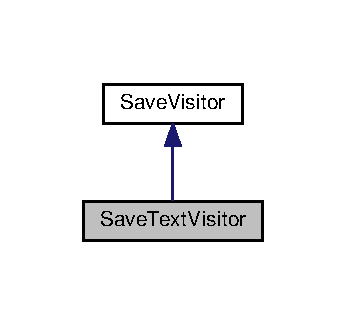
\includegraphics[width=166pt]{class_save_text_visitor__inherit__graph}
\end{center}
\end{figure}


Collaboration diagram for Save\+Text\+Visitor\+:\nopagebreak
\begin{figure}[H]
\begin{center}
\leavevmode
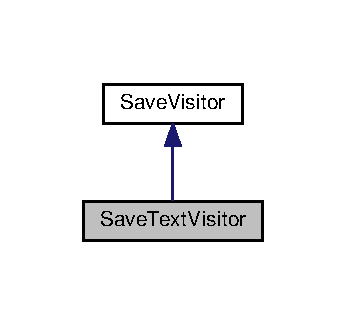
\includegraphics[width=166pt]{class_save_text_visitor__coll__graph}
\end{center}
\end{figure}
\subsection*{Public Member Functions}
\begin{DoxyCompactItemize}
\item 
\hyperlink{class_save_text_visitor_ae1ae492c0dd3eb6f26f4981a871d1130}{Save\+Text\+Visitor} ()
\item 
virtual \hyperlink{class_save_text_visitor_a1939db020915adce6354cc168cd1be3e}{$\sim$\+Save\+Text\+Visitor} ()
\item 
void \hyperlink{class_save_text_visitor_a2f083ffe6cda82e0c2fd31d601ba5e30}{save} (const \hyperlink{class_circle}{Circle} $\ast$circle, const string \&filename) const
\item 
void \hyperlink{class_save_text_visitor_aded2d7fe5898a3fd55bf4d15ed405416}{save} (const \hyperlink{class_segment}{Segment} $\ast$segment, const string \&filename) const
\item 
void \hyperlink{class_save_text_visitor_a1ac892a59b374572d44fc69b9b3528c0}{save} (const \hyperlink{class_triangle}{Triangle} $\ast$triangle, const string \&filename) const
\item 
void \hyperlink{class_save_text_visitor_a9b4292ce11779caf26556cf6abc5db0f}{save} (const \hyperlink{class_polygon}{Polygon} $\ast$polygon, const string \&filename) const
\item 
void \hyperlink{class_save_text_visitor_aa73d6b9e27e6b95d058c089fb4900514}{save} (const \hyperlink{class_shape}{Shape} $\ast$shape, const string \&filename) const
\end{DoxyCompactItemize}


\subsection{Detailed Description}
This class implements a way to save a shape in a simple text format. 

\subsection{Constructor \& Destructor Documentation}
\hypertarget{class_save_text_visitor_ae1ae492c0dd3eb6f26f4981a871d1130}{}\label{class_save_text_visitor_ae1ae492c0dd3eb6f26f4981a871d1130} 
\index{Save\+Text\+Visitor@{Save\+Text\+Visitor}!Save\+Text\+Visitor@{Save\+Text\+Visitor}}
\index{Save\+Text\+Visitor@{Save\+Text\+Visitor}!Save\+Text\+Visitor@{Save\+Text\+Visitor}}
\subsubsection{\texorpdfstring{Save\+Text\+Visitor()}{SaveTextVisitor()}}
{\footnotesize\ttfamily Save\+Text\+Visitor\+::\+Save\+Text\+Visitor (\begin{DoxyParamCaption}{ }\end{DoxyParamCaption})}

\hypertarget{class_save_text_visitor_a1939db020915adce6354cc168cd1be3e}{}\label{class_save_text_visitor_a1939db020915adce6354cc168cd1be3e} 
\index{Save\+Text\+Visitor@{Save\+Text\+Visitor}!````~Save\+Text\+Visitor@{$\sim$\+Save\+Text\+Visitor}}
\index{````~Save\+Text\+Visitor@{$\sim$\+Save\+Text\+Visitor}!Save\+Text\+Visitor@{Save\+Text\+Visitor}}
\subsubsection{\texorpdfstring{$\sim$\+Save\+Text\+Visitor()}{~SaveTextVisitor()}}
{\footnotesize\ttfamily Save\+Text\+Visitor\+::$\sim$\+Save\+Text\+Visitor (\begin{DoxyParamCaption}{ }\end{DoxyParamCaption})\hspace{0.3cm}{\ttfamily [virtual]}}



\subsection{Member Function Documentation}
\hypertarget{class_save_text_visitor_a2f083ffe6cda82e0c2fd31d601ba5e30}{}\label{class_save_text_visitor_a2f083ffe6cda82e0c2fd31d601ba5e30} 
\index{Save\+Text\+Visitor@{Save\+Text\+Visitor}!save@{save}}
\index{save@{save}!Save\+Text\+Visitor@{Save\+Text\+Visitor}}
\subsubsection{\texorpdfstring{save()}{save()}\hspace{0.1cm}{\footnotesize\ttfamily [1/5]}}
{\footnotesize\ttfamily void Save\+Text\+Visitor\+::save (\begin{DoxyParamCaption}\item[{const \hyperlink{class_circle}{Circle} $\ast$}]{circle,  }\item[{const string \&}]{filename }\end{DoxyParamCaption}) const\hspace{0.3cm}{\ttfamily [virtual]}}

Saves the \hyperlink{class_circle}{Circle}. 
\begin{DoxyParams}{Parameters}
{\em circle} & The \hyperlink{class_circle}{Circle} to save. \\
\hline
\end{DoxyParams}


Implements \hyperlink{class_save_visitor_a2e17acabc377913b745edb2b391052c7}{Save\+Visitor}.

\hypertarget{class_save_text_visitor_aded2d7fe5898a3fd55bf4d15ed405416}{}\label{class_save_text_visitor_aded2d7fe5898a3fd55bf4d15ed405416} 
\index{Save\+Text\+Visitor@{Save\+Text\+Visitor}!save@{save}}
\index{save@{save}!Save\+Text\+Visitor@{Save\+Text\+Visitor}}
\subsubsection{\texorpdfstring{save()}{save()}\hspace{0.1cm}{\footnotesize\ttfamily [2/5]}}
{\footnotesize\ttfamily void Save\+Text\+Visitor\+::save (\begin{DoxyParamCaption}\item[{const \hyperlink{class_segment}{Segment} $\ast$}]{segment,  }\item[{const string \&}]{filename }\end{DoxyParamCaption}) const\hspace{0.3cm}{\ttfamily [virtual]}}

Saves the \hyperlink{class_segment}{Segment}. 
\begin{DoxyParams}{Parameters}
{\em segment} & The \hyperlink{class_segment}{Segment} to save. \\
\hline
\end{DoxyParams}


Implements \hyperlink{class_save_visitor_ad23764257a2a9836cb920be85ecbcd64}{Save\+Visitor}.

\hypertarget{class_save_text_visitor_a1ac892a59b374572d44fc69b9b3528c0}{}\label{class_save_text_visitor_a1ac892a59b374572d44fc69b9b3528c0} 
\index{Save\+Text\+Visitor@{Save\+Text\+Visitor}!save@{save}}
\index{save@{save}!Save\+Text\+Visitor@{Save\+Text\+Visitor}}
\subsubsection{\texorpdfstring{save()}{save()}\hspace{0.1cm}{\footnotesize\ttfamily [3/5]}}
{\footnotesize\ttfamily void Save\+Text\+Visitor\+::save (\begin{DoxyParamCaption}\item[{const \hyperlink{class_triangle}{Triangle} $\ast$}]{triangle,  }\item[{const string \&}]{filename }\end{DoxyParamCaption}) const\hspace{0.3cm}{\ttfamily [virtual]}}

Saves the \hyperlink{class_triangle}{Triangle}. 
\begin{DoxyParams}{Parameters}
{\em triangle} & The \hyperlink{class_triangle}{Triangle} to save. \\
\hline
\end{DoxyParams}


Implements \hyperlink{class_save_visitor_aa94777a1d367e937294ffd467835dc31}{Save\+Visitor}.

\hypertarget{class_save_text_visitor_a9b4292ce11779caf26556cf6abc5db0f}{}\label{class_save_text_visitor_a9b4292ce11779caf26556cf6abc5db0f} 
\index{Save\+Text\+Visitor@{Save\+Text\+Visitor}!save@{save}}
\index{save@{save}!Save\+Text\+Visitor@{Save\+Text\+Visitor}}
\subsubsection{\texorpdfstring{save()}{save()}\hspace{0.1cm}{\footnotesize\ttfamily [4/5]}}
{\footnotesize\ttfamily void Save\+Text\+Visitor\+::save (\begin{DoxyParamCaption}\item[{const \hyperlink{class_polygon}{Polygon} $\ast$}]{polygon,  }\item[{const string \&}]{filename }\end{DoxyParamCaption}) const\hspace{0.3cm}{\ttfamily [virtual]}}

Saves the \hyperlink{class_polygon}{Polygon}. 
\begin{DoxyParams}{Parameters}
{\em polygon} & The \hyperlink{class_polygon}{Polygon} to save. \\
\hline
\end{DoxyParams}


Implements \hyperlink{class_save_visitor_aa24d8ccd081233a49ad31396e265af81}{Save\+Visitor}.

\hypertarget{class_save_text_visitor_aa73d6b9e27e6b95d058c089fb4900514}{}\label{class_save_text_visitor_aa73d6b9e27e6b95d058c089fb4900514} 
\index{Save\+Text\+Visitor@{Save\+Text\+Visitor}!save@{save}}
\index{save@{save}!Save\+Text\+Visitor@{Save\+Text\+Visitor}}
\subsubsection{\texorpdfstring{save()}{save()}\hspace{0.1cm}{\footnotesize\ttfamily [5/5]}}
{\footnotesize\ttfamily void Save\+Text\+Visitor\+::save (\begin{DoxyParamCaption}\item[{const \hyperlink{class_shape}{Shape} $\ast$}]{shape,  }\item[{const string \&}]{filename }\end{DoxyParamCaption}) const\hspace{0.3cm}{\ttfamily [virtual]}}

Saves the \hyperlink{class_shape}{Shape} 
\begin{DoxyParams}{Parameters}
{\em shape} & The \hyperlink{class_shape}{Shape} to save. \\
\hline
\end{DoxyParams}


Implements \hyperlink{class_save_visitor_a0d6549287b18302461912fe454a08af2}{Save\+Visitor}.



The documentation for this class was generated from the following files\+:\begin{DoxyCompactItemize}
\item 
src/\+Visitor/\hyperlink{_save_text_visitor_8hpp}{Save\+Text\+Visitor.\+hpp}\item 
src/\+Visitor/\hyperlink{_save_text_visitor_8cpp}{Save\+Text\+Visitor.\+cpp}\end{DoxyCompactItemize}

\hypertarget{class_save_visitor}{}\section{Save\+Visitor Class Reference}
\label{class_save_visitor}\index{Save\+Visitor@{Save\+Visitor}}


{\ttfamily \#include $<$Save\+Visitor.\+hpp$>$}



Inheritance diagram for Save\+Visitor\+:\nopagebreak
\begin{figure}[H]
\begin{center}
\leavevmode
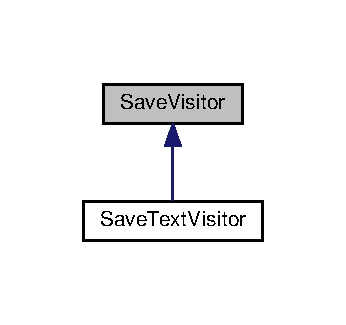
\includegraphics[width=166pt]{class_save_visitor__inherit__graph}
\end{center}
\end{figure}
\subsection*{Public Member Functions}
\begin{DoxyCompactItemize}
\item 
virtual void \hyperlink{class_save_visitor_a2e17acabc377913b745edb2b391052c7}{save} (const \hyperlink{class_circle}{Circle} $\ast$circle, const string \&filename) const =0
\item 
virtual void \hyperlink{class_save_visitor_ad23764257a2a9836cb920be85ecbcd64}{save} (const \hyperlink{class_segment}{Segment} $\ast$segment, const string \&filename) const =0
\item 
virtual void \hyperlink{class_save_visitor_aa94777a1d367e937294ffd467835dc31}{save} (const \hyperlink{class_triangle}{Triangle} $\ast$triangle, const string \&filename) const =0
\item 
virtual void \hyperlink{class_save_visitor_aa24d8ccd081233a49ad31396e265af81}{save} (const \hyperlink{class_polygon}{Polygon} $\ast$polygon, const string \&filename) const =0
\item 
virtual void \hyperlink{class_save_visitor_a0d6549287b18302461912fe454a08af2}{save} (const \hyperlink{class_shape}{Shape} $\ast$shape, const string \&filename) const =0
\end{DoxyCompactItemize}


\subsection{Detailed Description}
The abstract class to implement the classes that will save the Shapes. 

\subsection{Member Function Documentation}
\hypertarget{class_save_visitor_a2e17acabc377913b745edb2b391052c7}{}\label{class_save_visitor_a2e17acabc377913b745edb2b391052c7} 
\index{Save\+Visitor@{Save\+Visitor}!save@{save}}
\index{save@{save}!Save\+Visitor@{Save\+Visitor}}
\subsubsection{\texorpdfstring{save()}{save()}\hspace{0.1cm}{\footnotesize\ttfamily [1/5]}}
{\footnotesize\ttfamily virtual void Save\+Visitor\+::save (\begin{DoxyParamCaption}\item[{const \hyperlink{class_circle}{Circle} $\ast$}]{circle,  }\item[{const string \&}]{filename }\end{DoxyParamCaption}) const\hspace{0.3cm}{\ttfamily [pure virtual]}}

Saves the \hyperlink{class_circle}{Circle}. 
\begin{DoxyParams}{Parameters}
{\em circle} & The \hyperlink{class_circle}{Circle} to save. \\
\hline
\end{DoxyParams}


Implemented in \hyperlink{class_save_text_visitor_a2f083ffe6cda82e0c2fd31d601ba5e30}{Save\+Text\+Visitor}.

\hypertarget{class_save_visitor_ad23764257a2a9836cb920be85ecbcd64}{}\label{class_save_visitor_ad23764257a2a9836cb920be85ecbcd64} 
\index{Save\+Visitor@{Save\+Visitor}!save@{save}}
\index{save@{save}!Save\+Visitor@{Save\+Visitor}}
\subsubsection{\texorpdfstring{save()}{save()}\hspace{0.1cm}{\footnotesize\ttfamily [2/5]}}
{\footnotesize\ttfamily virtual void Save\+Visitor\+::save (\begin{DoxyParamCaption}\item[{const \hyperlink{class_segment}{Segment} $\ast$}]{segment,  }\item[{const string \&}]{filename }\end{DoxyParamCaption}) const\hspace{0.3cm}{\ttfamily [pure virtual]}}

Saves the \hyperlink{class_segment}{Segment}. 
\begin{DoxyParams}{Parameters}
{\em segment} & The \hyperlink{class_segment}{Segment} to save. \\
\hline
\end{DoxyParams}


Implemented in \hyperlink{class_save_text_visitor_aded2d7fe5898a3fd55bf4d15ed405416}{Save\+Text\+Visitor}.

\hypertarget{class_save_visitor_aa94777a1d367e937294ffd467835dc31}{}\label{class_save_visitor_aa94777a1d367e937294ffd467835dc31} 
\index{Save\+Visitor@{Save\+Visitor}!save@{save}}
\index{save@{save}!Save\+Visitor@{Save\+Visitor}}
\subsubsection{\texorpdfstring{save()}{save()}\hspace{0.1cm}{\footnotesize\ttfamily [3/5]}}
{\footnotesize\ttfamily virtual void Save\+Visitor\+::save (\begin{DoxyParamCaption}\item[{const \hyperlink{class_triangle}{Triangle} $\ast$}]{triangle,  }\item[{const string \&}]{filename }\end{DoxyParamCaption}) const\hspace{0.3cm}{\ttfamily [pure virtual]}}

Saves the \hyperlink{class_triangle}{Triangle}. 
\begin{DoxyParams}{Parameters}
{\em triangle} & The \hyperlink{class_triangle}{Triangle} to save. \\
\hline
\end{DoxyParams}


Implemented in \hyperlink{class_save_text_visitor_a1ac892a59b374572d44fc69b9b3528c0}{Save\+Text\+Visitor}.

\hypertarget{class_save_visitor_aa24d8ccd081233a49ad31396e265af81}{}\label{class_save_visitor_aa24d8ccd081233a49ad31396e265af81} 
\index{Save\+Visitor@{Save\+Visitor}!save@{save}}
\index{save@{save}!Save\+Visitor@{Save\+Visitor}}
\subsubsection{\texorpdfstring{save()}{save()}\hspace{0.1cm}{\footnotesize\ttfamily [4/5]}}
{\footnotesize\ttfamily virtual void Save\+Visitor\+::save (\begin{DoxyParamCaption}\item[{const \hyperlink{class_polygon}{Polygon} $\ast$}]{polygon,  }\item[{const string \&}]{filename }\end{DoxyParamCaption}) const\hspace{0.3cm}{\ttfamily [pure virtual]}}

Saves the \hyperlink{class_polygon}{Polygon}. 
\begin{DoxyParams}{Parameters}
{\em polygon} & The \hyperlink{class_polygon}{Polygon} to save. \\
\hline
\end{DoxyParams}


Implemented in \hyperlink{class_save_text_visitor_a9b4292ce11779caf26556cf6abc5db0f}{Save\+Text\+Visitor}.

\hypertarget{class_save_visitor_a0d6549287b18302461912fe454a08af2}{}\label{class_save_visitor_a0d6549287b18302461912fe454a08af2} 
\index{Save\+Visitor@{Save\+Visitor}!save@{save}}
\index{save@{save}!Save\+Visitor@{Save\+Visitor}}
\subsubsection{\texorpdfstring{save()}{save()}\hspace{0.1cm}{\footnotesize\ttfamily [5/5]}}
{\footnotesize\ttfamily virtual void Save\+Visitor\+::save (\begin{DoxyParamCaption}\item[{const \hyperlink{class_shape}{Shape} $\ast$}]{shape,  }\item[{const string \&}]{filename }\end{DoxyParamCaption}) const\hspace{0.3cm}{\ttfamily [pure virtual]}}

Saves the \hyperlink{class_shape}{Shape} 
\begin{DoxyParams}{Parameters}
{\em shape} & The \hyperlink{class_shape}{Shape} to save. \\
\hline
\end{DoxyParams}


Implemented in \hyperlink{class_save_text_visitor_aa73d6b9e27e6b95d058c089fb4900514}{Save\+Text\+Visitor}.



The documentation for this class was generated from the following file\+:\begin{DoxyCompactItemize}
\item 
src/\+Visitor/\hyperlink{_save_visitor_8hpp}{Save\+Visitor.\+hpp}\end{DoxyCompactItemize}

\hypertarget{class_segment}{}\section{Segment Class Reference}
\label{class_segment}\index{Segment@{Segment}}


{\ttfamily \#include $<$Segment.\+hpp$>$}



Inheritance diagram for Segment\+:\nopagebreak
\begin{figure}[H]
\begin{center}
\leavevmode
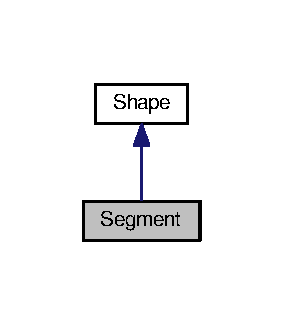
\includegraphics[width=136pt]{class_segment__inherit__graph}
\end{center}
\end{figure}


Collaboration diagram for Segment\+:\nopagebreak
\begin{figure}[H]
\begin{center}
\leavevmode
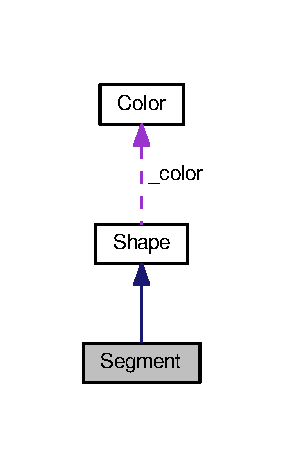
\includegraphics[width=138pt]{class_segment__coll__graph}
\end{center}
\end{figure}
\subsection*{Public Member Functions}
\begin{DoxyCompactItemize}
\item 
\hyperlink{class_segment_a1ac49abbcc008ed6cb519c87a421375e}{Segment} (const \hyperlink{class_vector2_d}{Vector2D} \&first\+Point, const \hyperlink{class_vector2_d}{Vector2D} \&second\+Point, const \hyperlink{class_color}{Color} \&color=\hyperlink{class_color_a94697e8c9eb81124c5a7c1439e1e7348}{Color\+::get\+Color}(\char`\"{}black\char`\"{}))
\item 
const \hyperlink{class_vector2_d}{Vector2D} \hyperlink{class_segment_a6aaa2508c09b60520c402f6e1054be5c}{get\+First\+Point} () const
\item 
const \hyperlink{class_vector2_d}{Vector2D} \hyperlink{class_segment_a7d7d1e5fa25f759f6bf0912925c9e922}{get\+Second\+Point} () const
\item 
void \hyperlink{class_segment_ad7b3641fc3670b1fba9cd97c2c40e3ba}{draw} (\hyperlink{class_drawing_visitor}{Drawing\+Visitor} $\ast$visitor) const
\item 
\hyperlink{class_segment_a28b3be893a35a0d73574354752c147fd}{operator string} () const
\item 
void \hyperlink{class_segment_a76c475fb193a0d7bb987da60dfc88ccd}{save} (const \hyperlink{class_save_visitor}{Save\+Visitor} $\ast$save\+Visitor, const string \&filename) const
\item 
\hyperlink{class_shape}{Shape} $\ast$ \hyperlink{class_segment_a8592ee9b864b2ebc61ab1810fa7dc577}{translation} (const \hyperlink{class_vector2_d}{Vector2D} \&translation\+Vector) const
\item 
\hyperlink{class_shape}{Shape} $\ast$ \hyperlink{class_segment_a5fe8d9711a0d3405a8c4cf3270069ee3}{homothety} (const \hyperlink{class_vector2_d}{Vector2D} \&invariant\+Point, const double \&homothety\+Ratio) const
\item 
\hyperlink{class_shape}{Shape} $\ast$ \hyperlink{class_segment_a46c1007c530f9be37ee7637e4ffdbf57}{rotation} (const \hyperlink{class_vector2_d}{Vector2D} \&rotation\+Center, const \hyperlink{class_radian_angle}{Radian\+Angle} \&rotation\+Angle) const
\item 
double \hyperlink{class_segment_af019f332cb32a21a1f9b7ae5acd7b4e7}{get\+Area} () const
\end{DoxyCompactItemize}
\subsection*{Friends}
\begin{DoxyCompactItemize}
\item 
ostream \& \hyperlink{class_segment_a8071236184a6b1617c06f5e5742f25a7}{operator$<$$<$} (ostream \&os, const \hyperlink{class_segment}{Segment} \&segment)
\end{DoxyCompactItemize}
\subsection*{Additional Inherited Members}


\subsection{Detailed Description}
Represent a \hyperlink{class_segment}{Segment} It\textquotesingle{}s a \hyperlink{class_shape}{Shape} 

\subsection{Constructor \& Destructor Documentation}
\hypertarget{class_segment_a1ac49abbcc008ed6cb519c87a421375e}{}\label{class_segment_a1ac49abbcc008ed6cb519c87a421375e} 
\index{Segment@{Segment}!Segment@{Segment}}
\index{Segment@{Segment}!Segment@{Segment}}
\subsubsection{\texorpdfstring{Segment()}{Segment()}}
{\footnotesize\ttfamily Segment\+::\+Segment (\begin{DoxyParamCaption}\item[{const \hyperlink{class_vector2_d}{Vector2D} \&}]{first\+Point,  }\item[{const \hyperlink{class_vector2_d}{Vector2D} \&}]{second\+Point,  }\item[{const \hyperlink{class_color}{Color} \&}]{color = {\ttfamily \hyperlink{class_color_a94697e8c9eb81124c5a7c1439e1e7348}{Color\+::get\+Color}(\char`\"{}black\char`\"{})} }\end{DoxyParamCaption})}

\hyperlink{class_segment}{Segment} constructor with color 
\begin{DoxyParams}{Parameters}
{\em first\+Point} & the first\+Point of the \hyperlink{class_segment}{Segment} \\
\hline
{\em second\+Point} & the second\+Point of the \hyperlink{class_segment}{Segment} \\
\hline
{\em color} & the color of the \hyperlink{class_segment}{Segment} \\
\hline
\end{DoxyParams}


\subsection{Member Function Documentation}
\hypertarget{class_segment_ad7b3641fc3670b1fba9cd97c2c40e3ba}{}\label{class_segment_ad7b3641fc3670b1fba9cd97c2c40e3ba} 
\index{Segment@{Segment}!draw@{draw}}
\index{draw@{draw}!Segment@{Segment}}
\subsubsection{\texorpdfstring{draw()}{draw()}}
{\footnotesize\ttfamily void Segment\+::draw (\begin{DoxyParamCaption}\item[{\hyperlink{class_drawing_visitor}{Drawing\+Visitor} $\ast$}]{visitor }\end{DoxyParamCaption}) const\hspace{0.3cm}{\ttfamily [virtual]}}

Draws the \hyperlink{class_segment}{Segment} using a \hyperlink{class_drawing_visitor}{Drawing\+Visitor}. 
\begin{DoxyParams}{Parameters}
{\em visitor} & The \hyperlink{class_drawing_visitor}{Drawing\+Visitor} to use to draw the \hyperlink{class_segment}{Segment}. \\
\hline
\end{DoxyParams}


Implements \hyperlink{class_shape_ae67fc6d39dd33759b65ff6112b21eab7}{Shape}.

\hypertarget{class_segment_af019f332cb32a21a1f9b7ae5acd7b4e7}{}\label{class_segment_af019f332cb32a21a1f9b7ae5acd7b4e7} 
\index{Segment@{Segment}!get\+Area@{get\+Area}}
\index{get\+Area@{get\+Area}!Segment@{Segment}}
\subsubsection{\texorpdfstring{get\+Area()}{getArea()}}
{\footnotesize\ttfamily double Segment\+::get\+Area (\begin{DoxyParamCaption}{ }\end{DoxyParamCaption}) const\hspace{0.3cm}{\ttfamily [virtual]}}

Returns the area of the \hyperlink{class_segment}{Segment}. \begin{DoxyReturn}{Returns}
The area of the \hyperlink{class_segment}{Segment}. 
\end{DoxyReturn}


Implements \hyperlink{class_shape_ad9454ee04617290547e7529180b1beae}{Shape}.

\hypertarget{class_segment_a6aaa2508c09b60520c402f6e1054be5c}{}\label{class_segment_a6aaa2508c09b60520c402f6e1054be5c} 
\index{Segment@{Segment}!get\+First\+Point@{get\+First\+Point}}
\index{get\+First\+Point@{get\+First\+Point}!Segment@{Segment}}
\subsubsection{\texorpdfstring{get\+First\+Point()}{getFirstPoint()}}
{\footnotesize\ttfamily const \hyperlink{class_vector2_d}{Vector2D} Segment\+::get\+First\+Point (\begin{DoxyParamCaption}{ }\end{DoxyParamCaption}) const}

Getter of the first point \begin{DoxyReturn}{Returns}
\hyperlink{class_vector2_d}{Vector2D} The first point 
\end{DoxyReturn}
\hypertarget{class_segment_a7d7d1e5fa25f759f6bf0912925c9e922}{}\label{class_segment_a7d7d1e5fa25f759f6bf0912925c9e922} 
\index{Segment@{Segment}!get\+Second\+Point@{get\+Second\+Point}}
\index{get\+Second\+Point@{get\+Second\+Point}!Segment@{Segment}}
\subsubsection{\texorpdfstring{get\+Second\+Point()}{getSecondPoint()}}
{\footnotesize\ttfamily const \hyperlink{class_vector2_d}{Vector2D} Segment\+::get\+Second\+Point (\begin{DoxyParamCaption}{ }\end{DoxyParamCaption}) const}

Getter of the second point \begin{DoxyReturn}{Returns}
\hyperlink{class_vector2_d}{Vector2D} The second point 
\end{DoxyReturn}
\hypertarget{class_segment_a5fe8d9711a0d3405a8c4cf3270069ee3}{}\label{class_segment_a5fe8d9711a0d3405a8c4cf3270069ee3} 
\index{Segment@{Segment}!homothety@{homothety}}
\index{homothety@{homothety}!Segment@{Segment}}
\subsubsection{\texorpdfstring{homothety()}{homothety()}}
{\footnotesize\ttfamily \hyperlink{class_shape}{Shape} $\ast$ Segment\+::homothety (\begin{DoxyParamCaption}\item[{const \hyperlink{class_vector2_d}{Vector2D} \&}]{invariant\+Point,  }\item[{const double \&}]{homothety\+Ratio }\end{DoxyParamCaption}) const\hspace{0.3cm}{\ttfamily [virtual]}}

Apply an homothety on the \hyperlink{class_segment}{Segment}. 
\begin{DoxyParams}{Parameters}
{\em invariant\+Point} & The center of the homothety. \\
\hline
{\em homothety\+Ratio} & The ratio of the homothety. \\
\hline
\end{DoxyParams}
\begin{DoxyReturn}{Returns}
Shape$\ast$ the new \hyperlink{class_segment}{Segment} after the homothety 
\end{DoxyReturn}


Implements \hyperlink{class_shape_a91f18af3004ba210db5c91084c50beb9}{Shape}.

\hypertarget{class_segment_a28b3be893a35a0d73574354752c147fd}{}\label{class_segment_a28b3be893a35a0d73574354752c147fd} 
\index{Segment@{Segment}!operator string@{operator string}}
\index{operator string@{operator string}!Segment@{Segment}}
\subsubsection{\texorpdfstring{operator string()}{operator string()}}
{\footnotesize\ttfamily Segment\+::operator string (\begin{DoxyParamCaption}{ }\end{DoxyParamCaption}) const\hspace{0.3cm}{\ttfamily [virtual]}}

Returns a string that represents the \hyperlink{class_segment}{Segment}. \begin{DoxyReturn}{Returns}
The string representing the \hyperlink{class_segment}{Segment}. 
\end{DoxyReturn}


Implements \hyperlink{class_shape_a0d74dcb2db0791b88b92f439bf4a6972}{Shape}.

\hypertarget{class_segment_a46c1007c530f9be37ee7637e4ffdbf57}{}\label{class_segment_a46c1007c530f9be37ee7637e4ffdbf57} 
\index{Segment@{Segment}!rotation@{rotation}}
\index{rotation@{rotation}!Segment@{Segment}}
\subsubsection{\texorpdfstring{rotation()}{rotation()}}
{\footnotesize\ttfamily \hyperlink{class_shape}{Shape} $\ast$ Segment\+::rotation (\begin{DoxyParamCaption}\item[{const \hyperlink{class_vector2_d}{Vector2D} \&}]{rotation\+Center,  }\item[{const \hyperlink{class_radian_angle}{Radian\+Angle} \&}]{rotation\+Angle }\end{DoxyParamCaption}) const\hspace{0.3cm}{\ttfamily [virtual]}}

Rotates the \hyperlink{class_segment}{Segment}. 
\begin{DoxyParams}{Parameters}
{\em rotation\+Center} & The center of the rotation. \\
\hline
{\em rotation\+Angle} & The angle of the rotation. \\
\hline
\end{DoxyParams}
\begin{DoxyReturn}{Returns}
Shape$\ast$ the new \hyperlink{class_segment}{Segment} after the rotation 
\end{DoxyReturn}


Implements \hyperlink{class_shape_abfc7a673b8a6d9a4d646dc15c771aa0d}{Shape}.

\hypertarget{class_segment_a76c475fb193a0d7bb987da60dfc88ccd}{}\label{class_segment_a76c475fb193a0d7bb987da60dfc88ccd} 
\index{Segment@{Segment}!save@{save}}
\index{save@{save}!Segment@{Segment}}
\subsubsection{\texorpdfstring{save()}{save()}}
{\footnotesize\ttfamily void Segment\+::save (\begin{DoxyParamCaption}\item[{const \hyperlink{class_save_visitor}{Save\+Visitor} $\ast$}]{save\+Visitor,  }\item[{const string \&}]{filename }\end{DoxyParamCaption}) const\hspace{0.3cm}{\ttfamily [virtual]}}

Saves the \hyperlink{class_segment}{Segment}. 
\begin{DoxyParams}{Parameters}
{\em save\+Visitor} & The \hyperlink{class_save_visitor}{Save\+Visitor} to use to save the \hyperlink{class_segment}{Segment}. \\
\hline
\end{DoxyParams}


Implements \hyperlink{class_shape_ae1477829e1b06aad805b8b76312f87bc}{Shape}.

\hypertarget{class_segment_a8592ee9b864b2ebc61ab1810fa7dc577}{}\label{class_segment_a8592ee9b864b2ebc61ab1810fa7dc577} 
\index{Segment@{Segment}!translation@{translation}}
\index{translation@{translation}!Segment@{Segment}}
\subsubsection{\texorpdfstring{translation()}{translation()}}
{\footnotesize\ttfamily \hyperlink{class_shape}{Shape} $\ast$ Segment\+::translation (\begin{DoxyParamCaption}\item[{const \hyperlink{class_vector2_d}{Vector2D} \&}]{translation\+Vector }\end{DoxyParamCaption}) const\hspace{0.3cm}{\ttfamily [virtual]}}

Translate the \hyperlink{class_segment}{Segment} using a translation vector. 
\begin{DoxyParams}{Parameters}
{\em translation\+Vector} & The translation vector to use for the translation. \\
\hline
\end{DoxyParams}
\begin{DoxyReturn}{Returns}
Shape$\ast$ the new \hyperlink{class_segment}{Segment} after the translation 
\end{DoxyReturn}


Implements \hyperlink{class_shape_ad3daca0d9bedf9aa15b92afab63c1de8}{Shape}.



\subsection{Friends And Related Function Documentation}
\hypertarget{class_segment_a8071236184a6b1617c06f5e5742f25a7}{}\label{class_segment_a8071236184a6b1617c06f5e5742f25a7} 
\index{Segment@{Segment}!operator$<$$<$@{operator$<$$<$}}
\index{operator$<$$<$@{operator$<$$<$}!Segment@{Segment}}
\subsubsection{\texorpdfstring{operator$<$$<$}{operator<<}}
{\footnotesize\ttfamily ostream\& operator$<$$<$ (\begin{DoxyParamCaption}\item[{ostream \&}]{os,  }\item[{const \hyperlink{class_segment}{Segment} \&}]{segment }\end{DoxyParamCaption})\hspace{0.3cm}{\ttfamily [friend]}}



The documentation for this class was generated from the following files\+:\begin{DoxyCompactItemize}
\item 
src/\+Shape/\hyperlink{_segment_8hpp}{Segment.\+hpp}\item 
src/\+Shape/\hyperlink{_segment_8cpp}{Segment.\+cpp}\end{DoxyCompactItemize}

\hypertarget{class_segment_creator}{}\section{Segment\+Creator Class Reference}
\label{class_segment_creator}\index{Segment\+Creator@{Segment\+Creator}}


{\ttfamily \#include $<$Segment\+Creator.\+hpp$>$}



Inheritance diagram for Segment\+Creator\+:\nopagebreak
\begin{figure}[H]
\begin{center}
\leavevmode
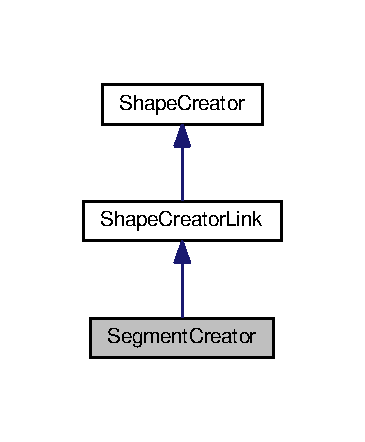
\includegraphics[width=175pt]{class_segment_creator__inherit__graph}
\end{center}
\end{figure}


Collaboration diagram for Segment\+Creator\+:\nopagebreak
\begin{figure}[H]
\begin{center}
\leavevmode
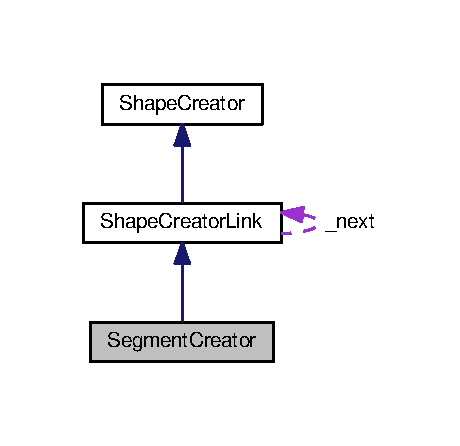
\includegraphics[width=221pt]{class_segment_creator__coll__graph}
\end{center}
\end{figure}
\subsection*{Public Member Functions}
\begin{DoxyCompactItemize}
\item 
\hyperlink{class_segment_creator_ad46fd18ef535e6eb4ccb7a1edbf906c8}{Segment\+Creator} (\hyperlink{class_shape_creator_link}{Shape\+Creator\+Link} $\ast$next)
\item 
virtual \hyperlink{class_shape}{Shape} $\ast$ \hyperlink{class_segment_creator_ab19a7665cba20a6e0b44c57b3cb4ce77}{create\+Shape\+Spe} (const string \&shape\+String) const
\end{DoxyCompactItemize}
\subsection*{Additional Inherited Members}


\subsection{Detailed Description}
Class \hyperlink{class_segment_creator}{Segment\+Creator} Link of the C\+OR for build \hyperlink{class_segment}{Segment} 

\subsection{Constructor \& Destructor Documentation}
\hypertarget{class_segment_creator_ad46fd18ef535e6eb4ccb7a1edbf906c8}{}\label{class_segment_creator_ad46fd18ef535e6eb4ccb7a1edbf906c8} 
\index{Segment\+Creator@{Segment\+Creator}!Segment\+Creator@{Segment\+Creator}}
\index{Segment\+Creator@{Segment\+Creator}!Segment\+Creator@{Segment\+Creator}}
\subsubsection{\texorpdfstring{Segment\+Creator()}{SegmentCreator()}}
{\footnotesize\ttfamily Segment\+Creator\+::\+Segment\+Creator (\begin{DoxyParamCaption}\item[{\hyperlink{class_shape_creator_link}{Shape\+Creator\+Link} $\ast$}]{next }\end{DoxyParamCaption})}

Constructor of \hyperlink{class_segment_creator}{Segment\+Creator} 
\begin{DoxyParams}{Parameters}
{\em next} & The next \hyperlink{class_shape_creator_link}{Shape\+Creator\+Link} if this one fails \\
\hline
\end{DoxyParams}


\subsection{Member Function Documentation}
\hypertarget{class_segment_creator_ab19a7665cba20a6e0b44c57b3cb4ce77}{}\label{class_segment_creator_ab19a7665cba20a6e0b44c57b3cb4ce77} 
\index{Segment\+Creator@{Segment\+Creator}!create\+Shape\+Spe@{create\+Shape\+Spe}}
\index{create\+Shape\+Spe@{create\+Shape\+Spe}!Segment\+Creator@{Segment\+Creator}}
\subsubsection{\texorpdfstring{create\+Shape\+Spe()}{createShapeSpe()}}
{\footnotesize\ttfamily \hyperlink{class_shape}{Shape} $\ast$ Segment\+Creator\+::create\+Shape\+Spe (\begin{DoxyParamCaption}\item[{const string \&}]{shape\+String }\end{DoxyParamCaption}) const\hspace{0.3cm}{\ttfamily [virtual]}}

Try to create a \hyperlink{class_segment}{Segment} with the string 
\begin{DoxyParams}{Parameters}
{\em shape\+String} & the string with informations of the shape \\
\hline
\end{DoxyParams}
\begin{DoxyReturn}{Returns}
The Shape$\ast$ wich were created 
\end{DoxyReturn}


Implements \hyperlink{class_shape_creator_link_a036ecc845946d23b36335e9077308bcf}{Shape\+Creator\+Link}.



The documentation for this class was generated from the following files\+:\begin{DoxyCompactItemize}
\item 
src/\+Loader/\hyperlink{_segment_creator_8hpp}{Segment\+Creator.\+hpp}\item 
src/\+Loader/\hyperlink{_segment_creator_8cpp}{Segment\+Creator.\+cpp}\end{DoxyCompactItemize}

\hypertarget{class_server_drawer}{}\section{Server\+Drawer Class Reference}
\label{class_server_drawer}\index{Server\+Drawer@{Server\+Drawer}}


{\ttfamily \#include $<$Server\+Drawer.\+hpp$>$}



Inheritance diagram for Server\+Drawer\+:\nopagebreak
\begin{figure}[H]
\begin{center}
\leavevmode
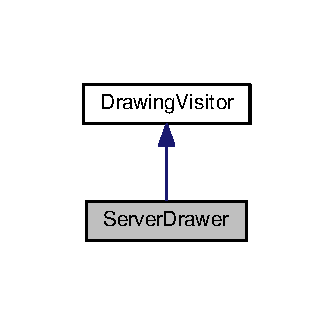
\includegraphics[width=160pt]{class_server_drawer__inherit__graph}
\end{center}
\end{figure}


Collaboration diagram for Server\+Drawer\+:\nopagebreak
\begin{figure}[H]
\begin{center}
\leavevmode
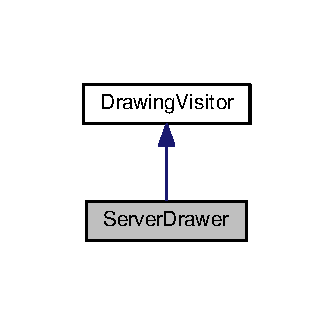
\includegraphics[width=160pt]{class_server_drawer__coll__graph}
\end{center}
\end{figure}
\subsection*{Public Member Functions}
\begin{DoxyCompactItemize}
\item 
\hyperlink{class_server_drawer_a533e227591169905b2b4eba7c6c3d3bc}{Server\+Drawer} ()
\item 
virtual \hyperlink{class_server_drawer_a40a7d8a070305d246bb12b23af81e72b}{$\sim$\+Server\+Drawer} ()
\item 
void \hyperlink{class_server_drawer_a70bd94ed93c913b53d689fb8fc5dddc9}{draw} (const \hyperlink{class_circle}{Circle} $\ast$circle)
\item 
void \hyperlink{class_server_drawer_a2bec9e70a1111d59b6c2d7de0908d780}{draw} (const \hyperlink{class_segment}{Segment} $\ast$segment)
\item 
void \hyperlink{class_server_drawer_aad913eff7f5c248003ef70ec8c09d2b2}{draw} (const \hyperlink{class_triangle}{Triangle} $\ast$triangle)
\item 
void \hyperlink{class_server_drawer_acd973f89e7618d67fcd8db364df0b6bf}{draw} (const \hyperlink{class_polygon}{Polygon} $\ast$polygon)
\item 
virtual void \hyperlink{class_server_drawer_a071fa49ab9edc71554b32aaaf7422b7f}{draw} (const \hyperlink{class_shape}{Shape} $\ast$shape)
\end{DoxyCompactItemize}


\subsection{Detailed Description}
This class is the drawer that implement a way to draw shapes using a drawing server. 

\subsection{Constructor \& Destructor Documentation}
\hypertarget{class_server_drawer_a533e227591169905b2b4eba7c6c3d3bc}{}\label{class_server_drawer_a533e227591169905b2b4eba7c6c3d3bc} 
\index{Server\+Drawer@{Server\+Drawer}!Server\+Drawer@{Server\+Drawer}}
\index{Server\+Drawer@{Server\+Drawer}!Server\+Drawer@{Server\+Drawer}}
\subsubsection{\texorpdfstring{Server\+Drawer()}{ServerDrawer()}}
{\footnotesize\ttfamily Server\+Drawer\+::\+Server\+Drawer (\begin{DoxyParamCaption}{ }\end{DoxyParamCaption})}

\hypertarget{class_server_drawer_a40a7d8a070305d246bb12b23af81e72b}{}\label{class_server_drawer_a40a7d8a070305d246bb12b23af81e72b} 
\index{Server\+Drawer@{Server\+Drawer}!````~Server\+Drawer@{$\sim$\+Server\+Drawer}}
\index{````~Server\+Drawer@{$\sim$\+Server\+Drawer}!Server\+Drawer@{Server\+Drawer}}
\subsubsection{\texorpdfstring{$\sim$\+Server\+Drawer()}{~ServerDrawer()}}
{\footnotesize\ttfamily Server\+Drawer\+::$\sim$\+Server\+Drawer (\begin{DoxyParamCaption}{ }\end{DoxyParamCaption})\hspace{0.3cm}{\ttfamily [virtual]}}



\subsection{Member Function Documentation}
\hypertarget{class_server_drawer_a70bd94ed93c913b53d689fb8fc5dddc9}{}\label{class_server_drawer_a70bd94ed93c913b53d689fb8fc5dddc9} 
\index{Server\+Drawer@{Server\+Drawer}!draw@{draw}}
\index{draw@{draw}!Server\+Drawer@{Server\+Drawer}}
\subsubsection{\texorpdfstring{draw()}{draw()}\hspace{0.1cm}{\footnotesize\ttfamily [1/5]}}
{\footnotesize\ttfamily void Server\+Drawer\+::draw (\begin{DoxyParamCaption}\item[{const \hyperlink{class_circle}{Circle} $\ast$}]{circle }\end{DoxyParamCaption})\hspace{0.3cm}{\ttfamily [virtual]}}

Draws the \hyperlink{class_circle}{Circle}. 
\begin{DoxyParams}{Parameters}
{\em circle} & The \hyperlink{class_circle}{Circle} to draw. \\
\hline
\end{DoxyParams}


Implements \hyperlink{class_drawing_visitor_a287f6d770c755c1c3bc144fb08b65030}{Drawing\+Visitor}.

\hypertarget{class_server_drawer_a2bec9e70a1111d59b6c2d7de0908d780}{}\label{class_server_drawer_a2bec9e70a1111d59b6c2d7de0908d780} 
\index{Server\+Drawer@{Server\+Drawer}!draw@{draw}}
\index{draw@{draw}!Server\+Drawer@{Server\+Drawer}}
\subsubsection{\texorpdfstring{draw()}{draw()}\hspace{0.1cm}{\footnotesize\ttfamily [2/5]}}
{\footnotesize\ttfamily void Server\+Drawer\+::draw (\begin{DoxyParamCaption}\item[{const \hyperlink{class_segment}{Segment} $\ast$}]{segment }\end{DoxyParamCaption})\hspace{0.3cm}{\ttfamily [virtual]}}

Draws the \hyperlink{class_segment}{Segment}. 
\begin{DoxyParams}{Parameters}
{\em segment} & The \hyperlink{class_segment}{Segment} to draw. \\
\hline
\end{DoxyParams}


Implements \hyperlink{class_drawing_visitor_a8a95018de31a7e3d7a067c347478ffde}{Drawing\+Visitor}.

\hypertarget{class_server_drawer_aad913eff7f5c248003ef70ec8c09d2b2}{}\label{class_server_drawer_aad913eff7f5c248003ef70ec8c09d2b2} 
\index{Server\+Drawer@{Server\+Drawer}!draw@{draw}}
\index{draw@{draw}!Server\+Drawer@{Server\+Drawer}}
\subsubsection{\texorpdfstring{draw()}{draw()}\hspace{0.1cm}{\footnotesize\ttfamily [3/5]}}
{\footnotesize\ttfamily void Server\+Drawer\+::draw (\begin{DoxyParamCaption}\item[{const \hyperlink{class_triangle}{Triangle} $\ast$}]{triangle }\end{DoxyParamCaption})\hspace{0.3cm}{\ttfamily [virtual]}}

Draws the \hyperlink{class_triangle}{Triangle}. 
\begin{DoxyParams}{Parameters}
{\em triangle} & The \hyperlink{class_triangle}{Triangle} to draw. \\
\hline
\end{DoxyParams}


Implements \hyperlink{class_drawing_visitor_a178aa7e1bb9cfbd538d7de0dbfa2d4b1}{Drawing\+Visitor}.

\hypertarget{class_server_drawer_acd973f89e7618d67fcd8db364df0b6bf}{}\label{class_server_drawer_acd973f89e7618d67fcd8db364df0b6bf} 
\index{Server\+Drawer@{Server\+Drawer}!draw@{draw}}
\index{draw@{draw}!Server\+Drawer@{Server\+Drawer}}
\subsubsection{\texorpdfstring{draw()}{draw()}\hspace{0.1cm}{\footnotesize\ttfamily [4/5]}}
{\footnotesize\ttfamily void Server\+Drawer\+::draw (\begin{DoxyParamCaption}\item[{const \hyperlink{class_polygon}{Polygon} $\ast$}]{polygon }\end{DoxyParamCaption})\hspace{0.3cm}{\ttfamily [virtual]}}

Draws the \hyperlink{class_polygon}{Polygon}. 
\begin{DoxyParams}{Parameters}
{\em polygon} & The \hyperlink{class_polygon}{Polygon} to draw. \\
\hline
\end{DoxyParams}


Implements \hyperlink{class_drawing_visitor_a771a2110a3afe4e87688bddd65657a46}{Drawing\+Visitor}.

\hypertarget{class_server_drawer_a071fa49ab9edc71554b32aaaf7422b7f}{}\label{class_server_drawer_a071fa49ab9edc71554b32aaaf7422b7f} 
\index{Server\+Drawer@{Server\+Drawer}!draw@{draw}}
\index{draw@{draw}!Server\+Drawer@{Server\+Drawer}}
\subsubsection{\texorpdfstring{draw()}{draw()}\hspace{0.1cm}{\footnotesize\ttfamily [5/5]}}
{\footnotesize\ttfamily void Server\+Drawer\+::draw (\begin{DoxyParamCaption}\item[{const \hyperlink{class_shape}{Shape} $\ast$}]{shape }\end{DoxyParamCaption})\hspace{0.3cm}{\ttfamily [virtual]}}

Draws the \hyperlink{class_shape}{Shape}. 
\begin{DoxyParams}{Parameters}
{\em polygon} & The \hyperlink{class_shape}{Shape} to draw. \\
\hline
\end{DoxyParams}


Implements \hyperlink{class_drawing_visitor_ad3d9e3028449f65ea2c405c74c4a55b4}{Drawing\+Visitor}.



The documentation for this class was generated from the following files\+:\begin{DoxyCompactItemize}
\item 
src/\+Visitor/\hyperlink{_server_drawer_8hpp}{Server\+Drawer.\+hpp}\item 
src/\+Visitor/\hyperlink{_server_drawer_8cpp}{Server\+Drawer.\+cpp}\end{DoxyCompactItemize}

\hypertarget{class_shape}{}\section{Shape Class Reference}
\label{class_shape}\index{Shape@{Shape}}


{\ttfamily \#include $<$Shape.\+hpp$>$}



Inheritance diagram for Shape\+:\nopagebreak
\begin{figure}[H]
\begin{center}
\leavevmode
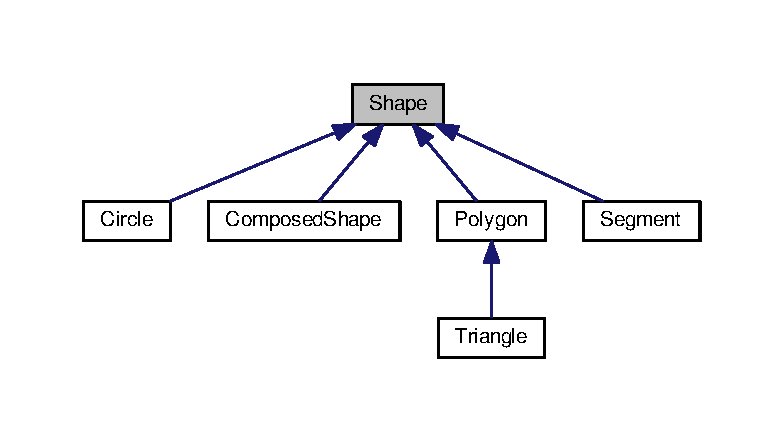
\includegraphics[width=350pt]{class_shape__inherit__graph}
\end{center}
\end{figure}


Collaboration diagram for Shape\+:\nopagebreak
\begin{figure}[H]
\begin{center}
\leavevmode
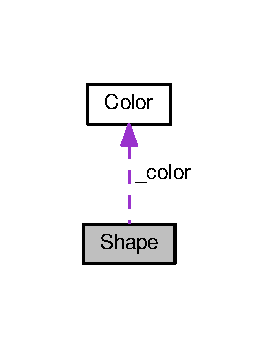
\includegraphics[width=132pt]{class_shape__coll__graph}
\end{center}
\end{figure}
\subsection*{Public Member Functions}
\begin{DoxyCompactItemize}
\item 
\hyperlink{class_shape_a6a2e4f913c228a1a167062035ba7e898}{Shape} (const \hyperlink{class_color}{Color} \&color=\hyperlink{class_color_a94697e8c9eb81124c5a7c1439e1e7348}{Color\+::get\+Color}(\char`\"{}black\char`\"{}))
\item 
virtual void \hyperlink{class_shape_ae67fc6d39dd33759b65ff6112b21eab7}{draw} (\hyperlink{class_drawing_visitor}{Drawing\+Visitor} $\ast$visitor) const =0
\item 
virtual \hyperlink{class_shape_a0d74dcb2db0791b88b92f439bf4a6972}{operator string} () const =0
\item 
virtual void \hyperlink{class_shape_ae1477829e1b06aad805b8b76312f87bc}{save} (const \hyperlink{class_save_visitor}{Save\+Visitor} $\ast$save\+Visitor, const string \&filename) const =0
\item 
virtual \hyperlink{class_shape}{Shape} $\ast$ \hyperlink{class_shape_ad3daca0d9bedf9aa15b92afab63c1de8}{translation} (const \hyperlink{class_vector2_d}{Vector2D} \&translation\+Vector) const =0
\item 
virtual \hyperlink{class_shape}{Shape} $\ast$ \hyperlink{class_shape_a91f18af3004ba210db5c91084c50beb9}{homothety} (const \hyperlink{class_vector2_d}{Vector2D} \&invariant\+Point, const double \&homothety\+Ratio) const =0
\item 
virtual \hyperlink{class_shape}{Shape} $\ast$ \hyperlink{class_shape_abfc7a673b8a6d9a4d646dc15c771aa0d}{rotation} (const \hyperlink{class_vector2_d}{Vector2D} \&rotation\+Center, const \hyperlink{class_radian_angle}{Radian\+Angle} \&rotation\+Angle) const =0
\item 
virtual double \hyperlink{class_shape_ad9454ee04617290547e7529180b1beae}{get\+Area} () const =0
\item 
virtual void \hyperlink{class_shape_a9f3d9c69476b41a375161b27949f765c}{set\+Color} (const \hyperlink{class_color}{Color} \&color)
\item 
virtual \hyperlink{class_color}{Color} \hyperlink{class_shape_a6ab685fc0e6aeec5d2e9743f5ecd66a4}{get\+Color} () const
\end{DoxyCompactItemize}
\subsection*{Protected Attributes}
\begin{DoxyCompactItemize}
\item 
\hyperlink{class_color}{Color} \hyperlink{class_shape_a5b499b01e45f0dbd8bbc64172f169213}{\+\_\+color}
\end{DoxyCompactItemize}
\subsection*{Friends}
\begin{DoxyCompactItemize}
\item 
ostream \& \hyperlink{class_shape_ada7f3e97b3113c4725bf7ec7293b5a36}{operator$<$$<$} (ostream \&os, const \hyperlink{class_shape}{Shape} \&shape)
\end{DoxyCompactItemize}


\subsection{Detailed Description}
This class is the base class for every \hyperlink{class_shape}{Shape}. 

\subsection{Constructor \& Destructor Documentation}
\hypertarget{class_shape_a6a2e4f913c228a1a167062035ba7e898}{}\label{class_shape_a6a2e4f913c228a1a167062035ba7e898} 
\index{Shape@{Shape}!Shape@{Shape}}
\index{Shape@{Shape}!Shape@{Shape}}
\subsubsection{\texorpdfstring{Shape()}{Shape()}}
{\footnotesize\ttfamily Shape\+::\+Shape (\begin{DoxyParamCaption}\item[{const \hyperlink{class_color}{Color} \&}]{color = {\ttfamily \hyperlink{class_color_a94697e8c9eb81124c5a7c1439e1e7348}{Color\+::get\+Color}(\char`\"{}black\char`\"{})} }\end{DoxyParamCaption})}



\subsection{Member Function Documentation}
\hypertarget{class_shape_ae67fc6d39dd33759b65ff6112b21eab7}{}\label{class_shape_ae67fc6d39dd33759b65ff6112b21eab7} 
\index{Shape@{Shape}!draw@{draw}}
\index{draw@{draw}!Shape@{Shape}}
\subsubsection{\texorpdfstring{draw()}{draw()}}
{\footnotesize\ttfamily virtual void Shape\+::draw (\begin{DoxyParamCaption}\item[{\hyperlink{class_drawing_visitor}{Drawing\+Visitor} $\ast$}]{visitor }\end{DoxyParamCaption}) const\hspace{0.3cm}{\ttfamily [pure virtual]}}

Draws the \hyperlink{class_shape}{Shape} using a \hyperlink{class_drawing_visitor}{Drawing\+Visitor}. 
\begin{DoxyParams}{Parameters}
{\em visitor} & The \hyperlink{class_drawing_visitor}{Drawing\+Visitor} to use to draw the shape. \\
\hline
\end{DoxyParams}


Implemented in \hyperlink{class_segment_ad7b3641fc3670b1fba9cd97c2c40e3ba}{Segment}, \hyperlink{class_polygon_a245c526a6a65ea99f5549fe5243006d0}{Polygon}, \hyperlink{class_triangle_a1fa834143ed718605959a227eba573b3}{Triangle}, \hyperlink{class_circle_a4c2dc8107eab8b562328743cafdddd79}{Circle}, and \hyperlink{class_composed_shape_a30f69734aa983bca56574ff4e5fd1723}{Composed\+Shape}.

\hypertarget{class_shape_ad9454ee04617290547e7529180b1beae}{}\label{class_shape_ad9454ee04617290547e7529180b1beae} 
\index{Shape@{Shape}!get\+Area@{get\+Area}}
\index{get\+Area@{get\+Area}!Shape@{Shape}}
\subsubsection{\texorpdfstring{get\+Area()}{getArea()}}
{\footnotesize\ttfamily virtual double Shape\+::get\+Area (\begin{DoxyParamCaption}{ }\end{DoxyParamCaption}) const\hspace{0.3cm}{\ttfamily [pure virtual]}}

Returns the area of the \hyperlink{class_shape}{Shape}. \begin{DoxyReturn}{Returns}
The area of the \hyperlink{class_shape}{Shape}. 
\end{DoxyReturn}


Implemented in \hyperlink{class_segment_af019f332cb32a21a1f9b7ae5acd7b4e7}{Segment}, \hyperlink{class_polygon_ae1ae9dd5e5613f119af3e31488427b01}{Polygon}, \hyperlink{class_triangle_a5f7fa9fd678345063e50e3458d943a9b}{Triangle}, \hyperlink{class_circle_a7bfb5ab5c8d4f11890407a2483ad61ee}{Circle}, and \hyperlink{class_composed_shape_a89b3457e1699afeb86805afad627d2c7}{Composed\+Shape}.

\hypertarget{class_shape_a6ab685fc0e6aeec5d2e9743f5ecd66a4}{}\label{class_shape_a6ab685fc0e6aeec5d2e9743f5ecd66a4} 
\index{Shape@{Shape}!get\+Color@{get\+Color}}
\index{get\+Color@{get\+Color}!Shape@{Shape}}
\subsubsection{\texorpdfstring{get\+Color()}{getColor()}}
{\footnotesize\ttfamily \hyperlink{class_color}{Color} Shape\+::get\+Color (\begin{DoxyParamCaption}{ }\end{DoxyParamCaption}) const\hspace{0.3cm}{\ttfamily [virtual]}}

Gets the color of the \hyperlink{class_shape}{Shape} \begin{DoxyReturn}{Returns}
The color of the \hyperlink{class_shape}{Shape}. 
\end{DoxyReturn}
\hypertarget{class_shape_a91f18af3004ba210db5c91084c50beb9}{}\label{class_shape_a91f18af3004ba210db5c91084c50beb9} 
\index{Shape@{Shape}!homothety@{homothety}}
\index{homothety@{homothety}!Shape@{Shape}}
\subsubsection{\texorpdfstring{homothety()}{homothety()}}
{\footnotesize\ttfamily virtual \hyperlink{class_shape}{Shape}$\ast$ Shape\+::homothety (\begin{DoxyParamCaption}\item[{const \hyperlink{class_vector2_d}{Vector2D} \&}]{invariant\+Point,  }\item[{const double \&}]{homothety\+Ratio }\end{DoxyParamCaption}) const\hspace{0.3cm}{\ttfamily [pure virtual]}}

Apply an homothety on the shape. 
\begin{DoxyParams}{Parameters}
{\em invariant\+Point} & The center of the homothety. \\
\hline
{\em homothety\+Ratio} & The ratio of the homothety. \\
\hline
\end{DoxyParams}


Implemented in \hyperlink{class_segment_a5fe8d9711a0d3405a8c4cf3270069ee3}{Segment}, \hyperlink{class_polygon_a2b77c7ecbe9ca68664d7f7020181b791}{Polygon}, \hyperlink{class_triangle_a45a3a9f74118c99b95c6d8e993773a71}{Triangle}, \hyperlink{class_circle_a031f188681977c2cf6ba2e80e30fb5ce}{Circle}, and \hyperlink{class_composed_shape_acff645310f05924aaf66b0de71b2307a}{Composed\+Shape}.

\hypertarget{class_shape_a0d74dcb2db0791b88b92f439bf4a6972}{}\label{class_shape_a0d74dcb2db0791b88b92f439bf4a6972} 
\index{Shape@{Shape}!operator string@{operator string}}
\index{operator string@{operator string}!Shape@{Shape}}
\subsubsection{\texorpdfstring{operator string()}{operator string()}}
{\footnotesize\ttfamily virtual Shape\+::operator string (\begin{DoxyParamCaption}{ }\end{DoxyParamCaption}) const\hspace{0.3cm}{\ttfamily [pure virtual]}}

Returns a string that represents the \hyperlink{class_shape}{Shape}. \begin{DoxyReturn}{Returns}
The string representing the \hyperlink{class_shape}{Shape}. 
\end{DoxyReturn}


Implemented in \hyperlink{class_segment_a28b3be893a35a0d73574354752c147fd}{Segment}, \hyperlink{class_polygon_a41c29b75f2463646af0f7bd604a4853d}{Polygon}, \hyperlink{class_triangle_acd8612cc20ffb71e543944c869e4ab81}{Triangle}, \hyperlink{class_circle_a4533a225b6d02699cea4045f47d3c7ff}{Circle}, and \hyperlink{class_composed_shape_aef491963b0e58209d1921973f2711c94}{Composed\+Shape}.

\hypertarget{class_shape_abfc7a673b8a6d9a4d646dc15c771aa0d}{}\label{class_shape_abfc7a673b8a6d9a4d646dc15c771aa0d} 
\index{Shape@{Shape}!rotation@{rotation}}
\index{rotation@{rotation}!Shape@{Shape}}
\subsubsection{\texorpdfstring{rotation()}{rotation()}}
{\footnotesize\ttfamily virtual \hyperlink{class_shape}{Shape}$\ast$ Shape\+::rotation (\begin{DoxyParamCaption}\item[{const \hyperlink{class_vector2_d}{Vector2D} \&}]{rotation\+Center,  }\item[{const \hyperlink{class_radian_angle}{Radian\+Angle} \&}]{rotation\+Angle }\end{DoxyParamCaption}) const\hspace{0.3cm}{\ttfamily [pure virtual]}}

Rotates the shape. 
\begin{DoxyParams}{Parameters}
{\em rotation\+Center} & The center of the rotation. \\
\hline
{\em rotation\+Angle} & The angle of the rotation. \\
\hline
\end{DoxyParams}


Implemented in \hyperlink{class_segment_a46c1007c530f9be37ee7637e4ffdbf57}{Segment}, \hyperlink{class_polygon_a5a453f01700f97ca98b0487cd670b194}{Polygon}, \hyperlink{class_triangle_a663ca3c6bd7967265849bf1f8c8a464b}{Triangle}, \hyperlink{class_circle_ac676105f9868877ffcecc9c236de10bb}{Circle}, and \hyperlink{class_composed_shape_a9c4f0561d631b20c6cd56348d41a14dd}{Composed\+Shape}.

\hypertarget{class_shape_ae1477829e1b06aad805b8b76312f87bc}{}\label{class_shape_ae1477829e1b06aad805b8b76312f87bc} 
\index{Shape@{Shape}!save@{save}}
\index{save@{save}!Shape@{Shape}}
\subsubsection{\texorpdfstring{save()}{save()}}
{\footnotesize\ttfamily virtual void Shape\+::save (\begin{DoxyParamCaption}\item[{const \hyperlink{class_save_visitor}{Save\+Visitor} $\ast$}]{save\+Visitor,  }\item[{const string \&}]{filename }\end{DoxyParamCaption}) const\hspace{0.3cm}{\ttfamily [pure virtual]}}

Saves the \hyperlink{class_shape}{Shape}. 
\begin{DoxyParams}{Parameters}
{\em save\+Visitor} & The \hyperlink{class_save_visitor}{Save\+Visitor} to use to save the shape. \\
\hline
\end{DoxyParams}


Implemented in \hyperlink{class_segment_a76c475fb193a0d7bb987da60dfc88ccd}{Segment}, \hyperlink{class_polygon_ad9adb867821b71e1aa8130dccbc9b37f}{Polygon}, \hyperlink{class_triangle_ae9ac3d633172f14d391d290a4467e1d3}{Triangle}, \hyperlink{class_circle_a91f2af619cc0465ae297ea88ce3b6c23}{Circle}, and \hyperlink{class_composed_shape_af189684eb5328b2fc13c694d7e637ff8}{Composed\+Shape}.

\hypertarget{class_shape_a9f3d9c69476b41a375161b27949f765c}{}\label{class_shape_a9f3d9c69476b41a375161b27949f765c} 
\index{Shape@{Shape}!set\+Color@{set\+Color}}
\index{set\+Color@{set\+Color}!Shape@{Shape}}
\subsubsection{\texorpdfstring{set\+Color()}{setColor()}}
{\footnotesize\ttfamily void Shape\+::set\+Color (\begin{DoxyParamCaption}\item[{const \hyperlink{class_color}{Color} \&}]{color }\end{DoxyParamCaption})\hspace{0.3cm}{\ttfamily [virtual]}}

Sets the color of the \hyperlink{class_shape}{Shape} 
\begin{DoxyParams}{Parameters}
{\em color} & The color of the \hyperlink{class_shape}{Shape}. \\
\hline
\end{DoxyParams}
\hypertarget{class_shape_ad3daca0d9bedf9aa15b92afab63c1de8}{}\label{class_shape_ad3daca0d9bedf9aa15b92afab63c1de8} 
\index{Shape@{Shape}!translation@{translation}}
\index{translation@{translation}!Shape@{Shape}}
\subsubsection{\texorpdfstring{translation()}{translation()}}
{\footnotesize\ttfamily virtual \hyperlink{class_shape}{Shape}$\ast$ Shape\+::translation (\begin{DoxyParamCaption}\item[{const \hyperlink{class_vector2_d}{Vector2D} \&}]{translation\+Vector }\end{DoxyParamCaption}) const\hspace{0.3cm}{\ttfamily [pure virtual]}}

Translate the shape using a translation vector. 
\begin{DoxyParams}{Parameters}
{\em translation\+Vector} & The translation vector to use for the translation. \\
\hline
\end{DoxyParams}


Implemented in \hyperlink{class_segment_a8592ee9b864b2ebc61ab1810fa7dc577}{Segment}, \hyperlink{class_polygon_ae828addfa5cffab547bcb16db1f275be}{Polygon}, \hyperlink{class_triangle_ac66208b0b633add41b915860f051cf44}{Triangle}, \hyperlink{class_circle_ad3b54b369f44baa1947aa3991f55e068}{Circle}, and \hyperlink{class_composed_shape_a31337a3fc33ac1fb929edbb6ff485dcc}{Composed\+Shape}.



\subsection{Friends And Related Function Documentation}
\hypertarget{class_shape_ada7f3e97b3113c4725bf7ec7293b5a36}{}\label{class_shape_ada7f3e97b3113c4725bf7ec7293b5a36} 
\index{Shape@{Shape}!operator$<$$<$@{operator$<$$<$}}
\index{operator$<$$<$@{operator$<$$<$}!Shape@{Shape}}
\subsubsection{\texorpdfstring{operator$<$$<$}{operator<<}}
{\footnotesize\ttfamily ostream\& operator$<$$<$ (\begin{DoxyParamCaption}\item[{ostream \&}]{os,  }\item[{const \hyperlink{class_shape}{Shape} \&}]{shape }\end{DoxyParamCaption})\hspace{0.3cm}{\ttfamily [friend]}}



\subsection{Member Data Documentation}
\hypertarget{class_shape_a5b499b01e45f0dbd8bbc64172f169213}{}\label{class_shape_a5b499b01e45f0dbd8bbc64172f169213} 
\index{Shape@{Shape}!\+\_\+color@{\+\_\+color}}
\index{\+\_\+color@{\+\_\+color}!Shape@{Shape}}
\subsubsection{\texorpdfstring{\+\_\+color}{\_color}}
{\footnotesize\ttfamily \hyperlink{class_color}{Color} Shape\+::\+\_\+color\hspace{0.3cm}{\ttfamily [protected]}}

Member \+\_\+color for color of the shape 

The documentation for this class was generated from the following files\+:\begin{DoxyCompactItemize}
\item 
src/\+Shape/\hyperlink{_shape_8hpp}{Shape.\+hpp}\item 
src/\+Shape/\hyperlink{_shape_8cpp}{Shape.\+cpp}\end{DoxyCompactItemize}

\hypertarget{class_shape_creator}{}\section{Shape\+Creator Class Reference}
\label{class_shape_creator}\index{Shape\+Creator@{Shape\+Creator}}


{\ttfamily \#include $<$Shape\+Creator.\+hpp$>$}



Inheritance diagram for Shape\+Creator\+:\nopagebreak
\begin{figure}[H]
\begin{center}
\leavevmode
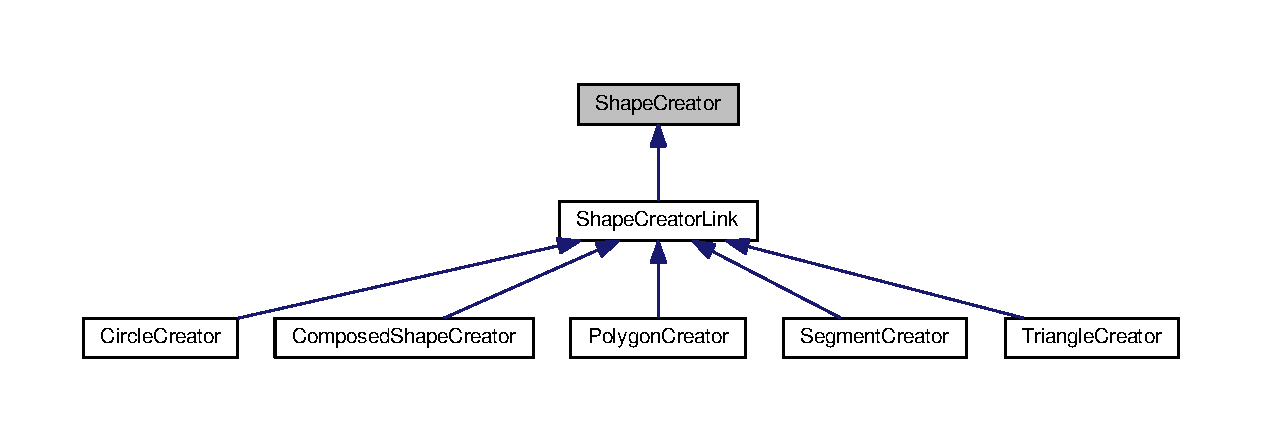
\includegraphics[width=350pt]{class_shape_creator__inherit__graph}
\end{center}
\end{figure}
\subsection*{Public Member Functions}
\begin{DoxyCompactItemize}
\item 
virtual \hyperlink{class_shape}{Shape} $\ast$ \hyperlink{class_shape_creator_a515bc403dc9de02b126d52480ba6ee78}{create\+Shape} (const string \&shape\+String) const =0
\end{DoxyCompactItemize}


\subsection{Detailed Description}
Abstract class \hyperlink{class_shape_creator}{Shape\+Creator} for handle shape creation C\+OR 

\subsection{Member Function Documentation}
\hypertarget{class_shape_creator_a515bc403dc9de02b126d52480ba6ee78}{}\label{class_shape_creator_a515bc403dc9de02b126d52480ba6ee78} 
\index{Shape\+Creator@{Shape\+Creator}!create\+Shape@{create\+Shape}}
\index{create\+Shape@{create\+Shape}!Shape\+Creator@{Shape\+Creator}}
\subsubsection{\texorpdfstring{create\+Shape()}{createShape()}}
{\footnotesize\ttfamily virtual \hyperlink{class_shape}{Shape}$\ast$ Shape\+Creator\+::create\+Shape (\begin{DoxyParamCaption}\item[{const string \&}]{shape\+String }\end{DoxyParamCaption}) const\hspace{0.3cm}{\ttfamily [pure virtual]}}

Virtual method for create a shape from a string 
\begin{DoxyParams}{Parameters}
{\em shape\+String} & The string cast of the shape have to create \\
\hline
\end{DoxyParams}
\begin{DoxyReturn}{Returns}
Shape$\ast$ The shape wich is create 
\end{DoxyReturn}


Implemented in \hyperlink{class_shape_creator_link_af372255e987c8fa587620e16dd406ccc}{Shape\+Creator\+Link}.



The documentation for this class was generated from the following file\+:\begin{DoxyCompactItemize}
\item 
src/\+Loader/\hyperlink{_shape_creator_8hpp}{Shape\+Creator.\+hpp}\end{DoxyCompactItemize}

\hypertarget{class_shape_creator_link}{}\section{Shape\+Creator\+Link Class Reference}
\label{class_shape_creator_link}\index{Shape\+Creator\+Link@{Shape\+Creator\+Link}}


{\ttfamily \#include $<$Shape\+Creator\+Link.\+hpp$>$}



Inheritance diagram for Shape\+Creator\+Link\+:\nopagebreak
\begin{figure}[H]
\begin{center}
\leavevmode
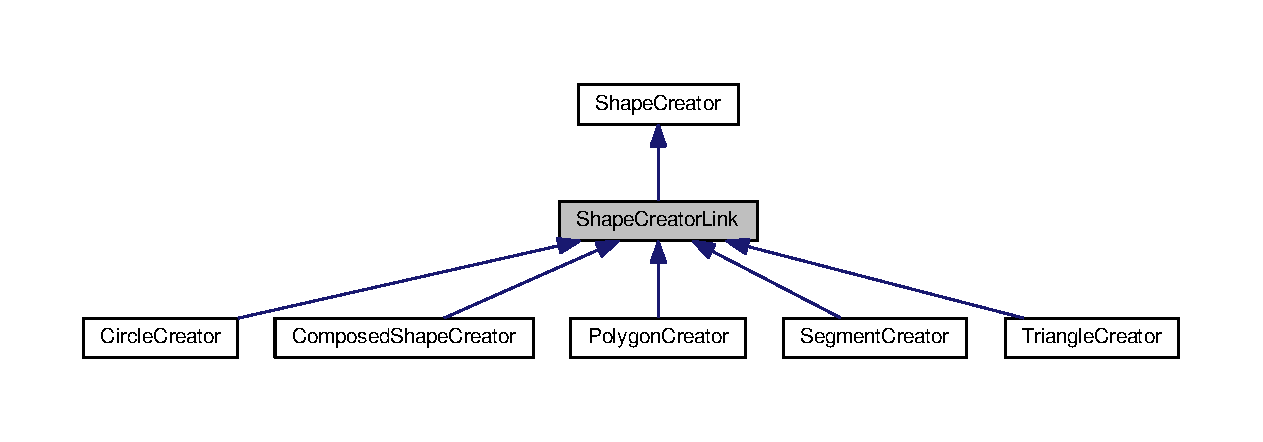
\includegraphics[width=350pt]{class_shape_creator_link__inherit__graph}
\end{center}
\end{figure}


Collaboration diagram for Shape\+Creator\+Link\+:\nopagebreak
\begin{figure}[H]
\begin{center}
\leavevmode
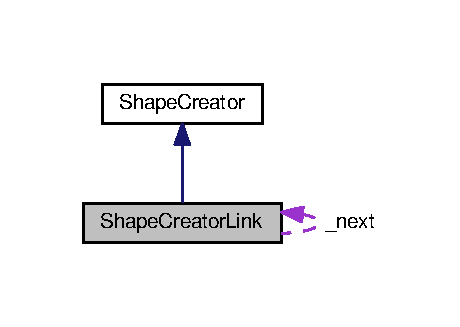
\includegraphics[width=221pt]{class_shape_creator_link__coll__graph}
\end{center}
\end{figure}
\subsection*{Public Member Functions}
\begin{DoxyCompactItemize}
\item 
\hyperlink{class_shape_creator_link_a625ba24fc48628d42ddd206e65489de0}{Shape\+Creator\+Link} (\hyperlink{class_shape_creator_link}{Shape\+Creator\+Link} $\ast$next)
\item 
\hyperlink{class_shape}{Shape} $\ast$ \hyperlink{class_shape_creator_link_af372255e987c8fa587620e16dd406ccc}{create\+Shape} (const string \&shape\+String) const
\item 
virtual \hyperlink{class_shape}{Shape} $\ast$ \hyperlink{class_shape_creator_link_a036ecc845946d23b36335e9077308bcf}{create\+Shape\+Spe} (const string \&shape\+String) const =0
\end{DoxyCompactItemize}
\subsection*{Protected Attributes}
\begin{DoxyCompactItemize}
\item 
\hyperlink{class_shape_creator_link}{Shape\+Creator\+Link} $\ast$ \hyperlink{class_shape_creator_link_a53714771bfbce43504eac24c4acf7e6f}{\+\_\+next}
\end{DoxyCompactItemize}


\subsection{Detailed Description}
Abstract class \hyperlink{class_shape_creator_link}{Shape\+Creator\+Link} for link the C\+OR of creation shape 

\subsection{Constructor \& Destructor Documentation}
\hypertarget{class_shape_creator_link_a625ba24fc48628d42ddd206e65489de0}{}\label{class_shape_creator_link_a625ba24fc48628d42ddd206e65489de0} 
\index{Shape\+Creator\+Link@{Shape\+Creator\+Link}!Shape\+Creator\+Link@{Shape\+Creator\+Link}}
\index{Shape\+Creator\+Link@{Shape\+Creator\+Link}!Shape\+Creator\+Link@{Shape\+Creator\+Link}}
\subsubsection{\texorpdfstring{Shape\+Creator\+Link()}{ShapeCreatorLink()}}
{\footnotesize\ttfamily Shape\+Creator\+Link\+::\+Shape\+Creator\+Link (\begin{DoxyParamCaption}\item[{\hyperlink{class_shape_creator_link}{Shape\+Creator\+Link} $\ast$}]{next }\end{DoxyParamCaption})}

Constructor of \hyperlink{class_shape_creator_link}{Shape\+Creator\+Link} 
\begin{DoxyParams}{Parameters}
{\em next} & A pointer of the next \hyperlink{class_shape_creator_link}{Shape\+Creator\+Link} \\
\hline
\end{DoxyParams}


\subsection{Member Function Documentation}
\hypertarget{class_shape_creator_link_af372255e987c8fa587620e16dd406ccc}{}\label{class_shape_creator_link_af372255e987c8fa587620e16dd406ccc} 
\index{Shape\+Creator\+Link@{Shape\+Creator\+Link}!create\+Shape@{create\+Shape}}
\index{create\+Shape@{create\+Shape}!Shape\+Creator\+Link@{Shape\+Creator\+Link}}
\subsubsection{\texorpdfstring{create\+Shape()}{createShape()}}
{\footnotesize\ttfamily \hyperlink{class_shape}{Shape} $\ast$ Shape\+Creator\+Link\+::create\+Shape (\begin{DoxyParamCaption}\item[{const string \&}]{shape\+String }\end{DoxyParamCaption}) const\hspace{0.3cm}{\ttfamily [virtual]}}

Try to create a shape with string If it doesn\textquotesingle{}t work, try with the next \hyperlink{class_shape_creator_link}{Shape\+Creator\+Link} 
\begin{DoxyParams}{Parameters}
{\em shape\+String} & The string for build the shape \\
\hline
\end{DoxyParams}
\begin{DoxyReturn}{Returns}
A Shape$\ast$ build with shape\+String 
\end{DoxyReturn}


Implements \hyperlink{class_shape_creator_a515bc403dc9de02b126d52480ba6ee78}{Shape\+Creator}.

\hypertarget{class_shape_creator_link_a036ecc845946d23b36335e9077308bcf}{}\label{class_shape_creator_link_a036ecc845946d23b36335e9077308bcf} 
\index{Shape\+Creator\+Link@{Shape\+Creator\+Link}!create\+Shape\+Spe@{create\+Shape\+Spe}}
\index{create\+Shape\+Spe@{create\+Shape\+Spe}!Shape\+Creator\+Link@{Shape\+Creator\+Link}}
\subsubsection{\texorpdfstring{create\+Shape\+Spe()}{createShapeSpe()}}
{\footnotesize\ttfamily virtual \hyperlink{class_shape}{Shape}$\ast$ Shape\+Creator\+Link\+::create\+Shape\+Spe (\begin{DoxyParamCaption}\item[{const string \&}]{shape\+String }\end{DoxyParamCaption}) const\hspace{0.3cm}{\ttfamily [pure virtual]}}

Abstract method for try creating shape with each type of \hyperlink{class_shape}{Shape} 
\begin{DoxyParams}{Parameters}
{\em shape\+String} & The string for build the shape \\
\hline
\end{DoxyParams}
\begin{DoxyReturn}{Returns}
A Shape$\ast$ build with shape\+String 
\end{DoxyReturn}


Implemented in \hyperlink{class_circle_creator_ae77dd120e2521fdfb2e002228a1f0c25}{Circle\+Creator}, \hyperlink{class_composed_shape_creator_a5a1ebce5d0d7509923e70d507dc57ff2}{Composed\+Shape\+Creator}, \hyperlink{class_polygon_creator_ad7a34580d4291a50fe189c912c7b32a0}{Polygon\+Creator}, \hyperlink{class_segment_creator_ab19a7665cba20a6e0b44c57b3cb4ce77}{Segment\+Creator}, and \hyperlink{class_triangle_creator_a8698d657d98a7be93aeaf86b2434bbb3}{Triangle\+Creator}.



\subsection{Member Data Documentation}
\hypertarget{class_shape_creator_link_a53714771bfbce43504eac24c4acf7e6f}{}\label{class_shape_creator_link_a53714771bfbce43504eac24c4acf7e6f} 
\index{Shape\+Creator\+Link@{Shape\+Creator\+Link}!\+\_\+next@{\+\_\+next}}
\index{\+\_\+next@{\+\_\+next}!Shape\+Creator\+Link@{Shape\+Creator\+Link}}
\subsubsection{\texorpdfstring{\+\_\+next}{\_next}}
{\footnotesize\ttfamily \hyperlink{class_shape_creator_link}{Shape\+Creator\+Link}$\ast$ Shape\+Creator\+Link\+::\+\_\+next\hspace{0.3cm}{\ttfamily [protected]}}



The documentation for this class was generated from the following files\+:\begin{DoxyCompactItemize}
\item 
src/\+Loader/\hyperlink{_shape_creator_link_8hpp}{Shape\+Creator\+Link.\+hpp}\item 
src/\+Loader/\hyperlink{_shape_creator_link_8cpp}{Shape\+Creator\+Link.\+cpp}\end{DoxyCompactItemize}

\hypertarget{class_shape_loader}{}\section{Shape\+Loader Class Reference}
\label{class_shape_loader}\index{Shape\+Loader@{Shape\+Loader}}


{\ttfamily \#include $<$Shape\+Loader.\+hpp$>$}



Inheritance diagram for Shape\+Loader\+:\nopagebreak
\begin{figure}[H]
\begin{center}
\leavevmode
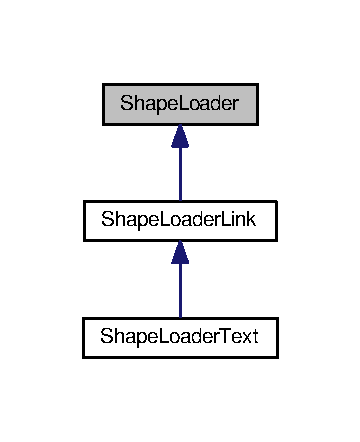
\includegraphics[width=173pt]{class_shape_loader__inherit__graph}
\end{center}
\end{figure}


Collaboration diagram for Shape\+Loader\+:\nopagebreak
\begin{figure}[H]
\begin{center}
\leavevmode
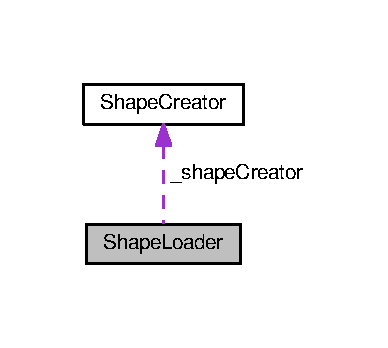
\includegraphics[width=186pt]{class_shape_loader__coll__graph}
\end{center}
\end{figure}
\subsection*{Public Member Functions}
\begin{DoxyCompactItemize}
\item 
\hyperlink{class_shape_loader_a648a5e0abfda168281769ae2c68e1d0b}{Shape\+Loader} (const \hyperlink{class_shape_creator}{Shape\+Creator} $\ast$shape\+Creator)
\item 
virtual \hyperlink{class_shape}{Shape} $\ast$ \hyperlink{class_shape_loader_af675cfe98578da47d31c54a3ea3748e1}{load} (const string \&filename) const =0
\end{DoxyCompactItemize}
\subsection*{Protected Attributes}
\begin{DoxyCompactItemize}
\item 
const \hyperlink{class_shape_creator}{Shape\+Creator} $\ast$ \hyperlink{class_shape_loader_ae412cdea4d16545ea9845870ec1e83e5}{\+\_\+shape\+Creator}
\end{DoxyCompactItemize}


\subsection{Constructor \& Destructor Documentation}
\hypertarget{class_shape_loader_a648a5e0abfda168281769ae2c68e1d0b}{}\label{class_shape_loader_a648a5e0abfda168281769ae2c68e1d0b} 
\index{Shape\+Loader@{Shape\+Loader}!Shape\+Loader@{Shape\+Loader}}
\index{Shape\+Loader@{Shape\+Loader}!Shape\+Loader@{Shape\+Loader}}
\subsubsection{\texorpdfstring{Shape\+Loader()}{ShapeLoader()}}
{\footnotesize\ttfamily Shape\+Loader\+::\+Shape\+Loader (\begin{DoxyParamCaption}\item[{const \hyperlink{class_shape_creator}{Shape\+Creator} $\ast$}]{shape\+Creator }\end{DoxyParamCaption})\hspace{0.3cm}{\ttfamily [inline]}}



\subsection{Member Function Documentation}
\hypertarget{class_shape_loader_af675cfe98578da47d31c54a3ea3748e1}{}\label{class_shape_loader_af675cfe98578da47d31c54a3ea3748e1} 
\index{Shape\+Loader@{Shape\+Loader}!load@{load}}
\index{load@{load}!Shape\+Loader@{Shape\+Loader}}
\subsubsection{\texorpdfstring{load()}{load()}}
{\footnotesize\ttfamily virtual \hyperlink{class_shape}{Shape}$\ast$ Shape\+Loader\+::load (\begin{DoxyParamCaption}\item[{const string \&}]{filename }\end{DoxyParamCaption}) const\hspace{0.3cm}{\ttfamily [pure virtual]}}



Implemented in \hyperlink{class_shape_loader_link_a0637abbe648488e98f4130bd9827bd72}{Shape\+Loader\+Link}.



\subsection{Member Data Documentation}
\hypertarget{class_shape_loader_ae412cdea4d16545ea9845870ec1e83e5}{}\label{class_shape_loader_ae412cdea4d16545ea9845870ec1e83e5} 
\index{Shape\+Loader@{Shape\+Loader}!\+\_\+shape\+Creator@{\+\_\+shape\+Creator}}
\index{\+\_\+shape\+Creator@{\+\_\+shape\+Creator}!Shape\+Loader@{Shape\+Loader}}
\subsubsection{\texorpdfstring{\+\_\+shape\+Creator}{\_shapeCreator}}
{\footnotesize\ttfamily const \hyperlink{class_shape_creator}{Shape\+Creator}$\ast$ Shape\+Loader\+::\+\_\+shape\+Creator\hspace{0.3cm}{\ttfamily [protected]}}



The documentation for this class was generated from the following file\+:\begin{DoxyCompactItemize}
\item 
src/\+Loader/\hyperlink{_shape_loader_8hpp}{Shape\+Loader.\+hpp}\end{DoxyCompactItemize}

\hypertarget{class_shape_loader_exception}{}\section{Shape\+Loader\+Exception Class Reference}
\label{class_shape_loader_exception}\index{Shape\+Loader\+Exception@{Shape\+Loader\+Exception}}


{\ttfamily \#include $<$Shape\+Loader\+Exception.\+hpp$>$}

\subsection*{Public Member Functions}
\begin{DoxyCompactItemize}
\item 
\hyperlink{class_shape_loader_exception_abafaa24f3865b9a1bc5a0c3b4ffb62b5}{Shape\+Loader\+Exception} (const string \&message)
\end{DoxyCompactItemize}
\subsection*{Friends}
\begin{DoxyCompactItemize}
\item 
ostream \& \hyperlink{class_shape_loader_exception_aaeb686a05fcc919d9b383b9f61182f44}{operator$<$$<$} (ostream \&os, const \hyperlink{class_shape_loader_exception}{Shape\+Loader\+Exception} \&shape\+Loader\+Exception)
\end{DoxyCompactItemize}


\subsection{Detailed Description}
Class for hander all network exceptions 

\subsection{Constructor \& Destructor Documentation}
\hypertarget{class_shape_loader_exception_abafaa24f3865b9a1bc5a0c3b4ffb62b5}{}\label{class_shape_loader_exception_abafaa24f3865b9a1bc5a0c3b4ffb62b5} 
\index{Shape\+Loader\+Exception@{Shape\+Loader\+Exception}!Shape\+Loader\+Exception@{Shape\+Loader\+Exception}}
\index{Shape\+Loader\+Exception@{Shape\+Loader\+Exception}!Shape\+Loader\+Exception@{Shape\+Loader\+Exception}}
\subsubsection{\texorpdfstring{Shape\+Loader\+Exception()}{ShapeLoaderException()}}
{\footnotesize\ttfamily Shape\+Loader\+Exception\+::\+Shape\+Loader\+Exception (\begin{DoxyParamCaption}\item[{const string \&}]{message }\end{DoxyParamCaption})}

Constructor of \hyperlink{class_shape_loader_exception}{Shape\+Loader\+Exception} 
\begin{DoxyParams}{Parameters}
{\em message} & the message to throw \\
\hline
\end{DoxyParams}


\subsection{Friends And Related Function Documentation}
\hypertarget{class_shape_loader_exception_aaeb686a05fcc919d9b383b9f61182f44}{}\label{class_shape_loader_exception_aaeb686a05fcc919d9b383b9f61182f44} 
\index{Shape\+Loader\+Exception@{Shape\+Loader\+Exception}!operator$<$$<$@{operator$<$$<$}}
\index{operator$<$$<$@{operator$<$$<$}!Shape\+Loader\+Exception@{Shape\+Loader\+Exception}}
\subsubsection{\texorpdfstring{operator$<$$<$}{operator<<}}
{\footnotesize\ttfamily ostream\& operator$<$$<$ (\begin{DoxyParamCaption}\item[{ostream \&}]{os,  }\item[{const \hyperlink{class_shape_loader_exception}{Shape\+Loader\+Exception} \&}]{shape\+Loader\+Exception }\end{DoxyParamCaption})\hspace{0.3cm}{\ttfamily [friend]}}

Sends a string of excpetion to a stream 
\begin{DoxyParams}{Parameters}
{\em os} & ostream \\
\hline
{\em \hyperlink{class_shape_loader_exception}{Shape\+Loader\+Exception}} & \hyperlink{class_shape_loader_exception}{Shape\+Loader\+Exception} have to print \\
\hline
\end{DoxyParams}
\begin{DoxyReturn}{Returns}
ostream to send to the output 
\end{DoxyReturn}


The documentation for this class was generated from the following files\+:\begin{DoxyCompactItemize}
\item 
src/\+Loader/\hyperlink{_shape_loader_exception_8hpp}{Shape\+Loader\+Exception.\+hpp}\item 
src/\+Loader/\hyperlink{_shape_loader_exception_8cpp}{Shape\+Loader\+Exception.\+cpp}\end{DoxyCompactItemize}

\hypertarget{class_shape_loader_link}{}\section{Shape\+Loader\+Link Class Reference}
\label{class_shape_loader_link}\index{Shape\+Loader\+Link@{Shape\+Loader\+Link}}


{\ttfamily \#include $<$Shape\+Loader\+Link.\+hpp$>$}



Inheritance diagram for Shape\+Loader\+Link\+:\nopagebreak
\begin{figure}[H]
\begin{center}
\leavevmode
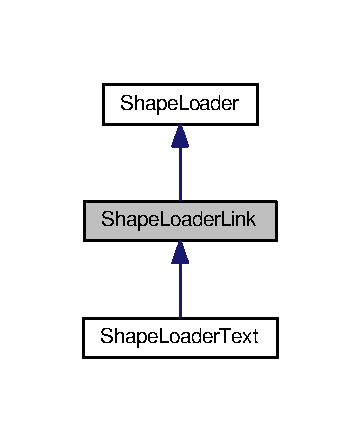
\includegraphics[width=173pt]{class_shape_loader_link__inherit__graph}
\end{center}
\end{figure}


Collaboration diagram for Shape\+Loader\+Link\+:\nopagebreak
\begin{figure}[H]
\begin{center}
\leavevmode
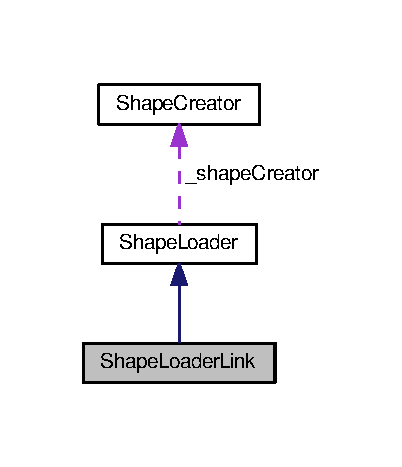
\includegraphics[width=193pt]{class_shape_loader_link__coll__graph}
\end{center}
\end{figure}
\subsection*{Public Member Functions}
\begin{DoxyCompactItemize}
\item 
\hyperlink{class_shape_loader_link_a79c836d9ee6912b2ad018f736264bc3b}{Shape\+Loader\+Link} (const \hyperlink{class_shape_loader_link}{Shape\+Loader\+Link} $\ast$next, const \hyperlink{class_shape_creator}{Shape\+Creator} $\ast$shape\+Creator)
\item 
virtual \hyperlink{class_shape_loader_link_ac1d209f646bb69bae5ba34d7ae132ba1}{$\sim$\+Shape\+Loader\+Link} ()
\item 
\hyperlink{class_shape}{Shape} $\ast$ \hyperlink{class_shape_loader_link_a0637abbe648488e98f4130bd9827bd72}{load} (const string \&filename) const
\item 
virtual \hyperlink{class_shape}{Shape} $\ast$ \hyperlink{class_shape_loader_link_a02f18caa405a1d5a1e24ed5b7bf08320}{load\+Shape} (const string \&filename) const =0
\end{DoxyCompactItemize}
\subsection*{Additional Inherited Members}


\subsection{Constructor \& Destructor Documentation}
\hypertarget{class_shape_loader_link_a79c836d9ee6912b2ad018f736264bc3b}{}\label{class_shape_loader_link_a79c836d9ee6912b2ad018f736264bc3b} 
\index{Shape\+Loader\+Link@{Shape\+Loader\+Link}!Shape\+Loader\+Link@{Shape\+Loader\+Link}}
\index{Shape\+Loader\+Link@{Shape\+Loader\+Link}!Shape\+Loader\+Link@{Shape\+Loader\+Link}}
\subsubsection{\texorpdfstring{Shape\+Loader\+Link()}{ShapeLoaderLink()}}
{\footnotesize\ttfamily Shape\+Loader\+Link\+::\+Shape\+Loader\+Link (\begin{DoxyParamCaption}\item[{const \hyperlink{class_shape_loader_link}{Shape\+Loader\+Link} $\ast$}]{next,  }\item[{const \hyperlink{class_shape_creator}{Shape\+Creator} $\ast$}]{shape\+Creator }\end{DoxyParamCaption})}

\hypertarget{class_shape_loader_link_ac1d209f646bb69bae5ba34d7ae132ba1}{}\label{class_shape_loader_link_ac1d209f646bb69bae5ba34d7ae132ba1} 
\index{Shape\+Loader\+Link@{Shape\+Loader\+Link}!````~Shape\+Loader\+Link@{$\sim$\+Shape\+Loader\+Link}}
\index{````~Shape\+Loader\+Link@{$\sim$\+Shape\+Loader\+Link}!Shape\+Loader\+Link@{Shape\+Loader\+Link}}
\subsubsection{\texorpdfstring{$\sim$\+Shape\+Loader\+Link()}{~ShapeLoaderLink()}}
{\footnotesize\ttfamily Shape\+Loader\+Link\+::$\sim$\+Shape\+Loader\+Link (\begin{DoxyParamCaption}{ }\end{DoxyParamCaption})\hspace{0.3cm}{\ttfamily [virtual]}}



\subsection{Member Function Documentation}
\hypertarget{class_shape_loader_link_a0637abbe648488e98f4130bd9827bd72}{}\label{class_shape_loader_link_a0637abbe648488e98f4130bd9827bd72} 
\index{Shape\+Loader\+Link@{Shape\+Loader\+Link}!load@{load}}
\index{load@{load}!Shape\+Loader\+Link@{Shape\+Loader\+Link}}
\subsubsection{\texorpdfstring{load()}{load()}}
{\footnotesize\ttfamily \hyperlink{class_shape}{Shape} $\ast$ Shape\+Loader\+Link\+::load (\begin{DoxyParamCaption}\item[{const string \&}]{filename }\end{DoxyParamCaption}) const\hspace{0.3cm}{\ttfamily [virtual]}}



Implements \hyperlink{class_shape_loader_af675cfe98578da47d31c54a3ea3748e1}{Shape\+Loader}.

\hypertarget{class_shape_loader_link_a02f18caa405a1d5a1e24ed5b7bf08320}{}\label{class_shape_loader_link_a02f18caa405a1d5a1e24ed5b7bf08320} 
\index{Shape\+Loader\+Link@{Shape\+Loader\+Link}!load\+Shape@{load\+Shape}}
\index{load\+Shape@{load\+Shape}!Shape\+Loader\+Link@{Shape\+Loader\+Link}}
\subsubsection{\texorpdfstring{load\+Shape()}{loadShape()}}
{\footnotesize\ttfamily virtual \hyperlink{class_shape}{Shape}$\ast$ Shape\+Loader\+Link\+::load\+Shape (\begin{DoxyParamCaption}\item[{const string \&}]{filename }\end{DoxyParamCaption}) const\hspace{0.3cm}{\ttfamily [pure virtual]}}



Implemented in \hyperlink{class_shape_loader_text_a7770dff8a2b7c942e2fdf5b5c15b5748}{Shape\+Loader\+Text}.



The documentation for this class was generated from the following files\+:\begin{DoxyCompactItemize}
\item 
src/\+Loader/\hyperlink{_shape_loader_link_8hpp}{Shape\+Loader\+Link.\+hpp}\item 
src/\+Loader/\hyperlink{_shape_loader_link_8cpp}{Shape\+Loader\+Link.\+cpp}\end{DoxyCompactItemize}

\hypertarget{class_shape_loader_text}{}\section{Shape\+Loader\+Text Class Reference}
\label{class_shape_loader_text}\index{Shape\+Loader\+Text@{Shape\+Loader\+Text}}


{\ttfamily \#include $<$Shape\+Loader\+Text.\+hpp$>$}



Inheritance diagram for Shape\+Loader\+Text\+:\nopagebreak
\begin{figure}[H]
\begin{center}
\leavevmode
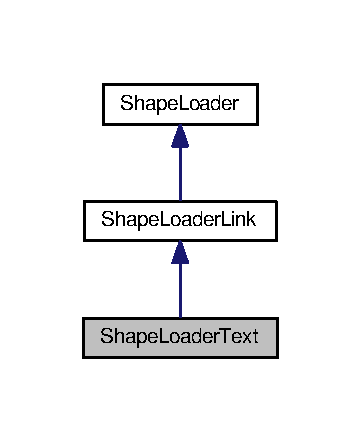
\includegraphics[width=173pt]{class_shape_loader_text__inherit__graph}
\end{center}
\end{figure}


Collaboration diagram for Shape\+Loader\+Text\+:\nopagebreak
\begin{figure}[H]
\begin{center}
\leavevmode
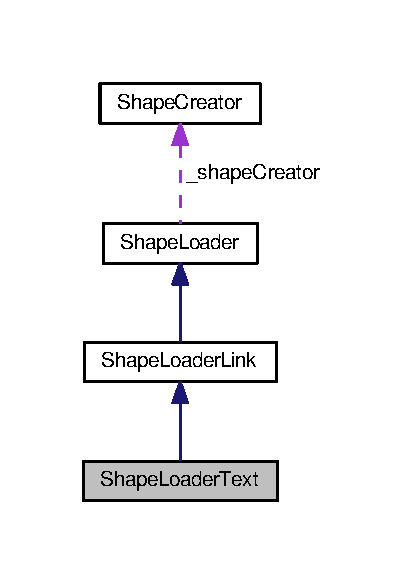
\includegraphics[width=194pt]{class_shape_loader_text__coll__graph}
\end{center}
\end{figure}
\subsection*{Public Member Functions}
\begin{DoxyCompactItemize}
\item 
\hyperlink{class_shape_loader_text_ac2bbc1cc5d177966949935a008016b57}{Shape\+Loader\+Text} (const \hyperlink{class_shape_loader_link}{Shape\+Loader\+Link} $\ast$next, const \hyperlink{class_shape_creator}{Shape\+Creator} $\ast$shape\+Creator)
\item 
\hyperlink{class_shape}{Shape} $\ast$ \hyperlink{class_shape_loader_text_a7770dff8a2b7c942e2fdf5b5c15b5748}{load\+Shape} (const string \&filename) const
\end{DoxyCompactItemize}
\subsection*{Additional Inherited Members}


\subsection{Constructor \& Destructor Documentation}
\hypertarget{class_shape_loader_text_ac2bbc1cc5d177966949935a008016b57}{}\label{class_shape_loader_text_ac2bbc1cc5d177966949935a008016b57} 
\index{Shape\+Loader\+Text@{Shape\+Loader\+Text}!Shape\+Loader\+Text@{Shape\+Loader\+Text}}
\index{Shape\+Loader\+Text@{Shape\+Loader\+Text}!Shape\+Loader\+Text@{Shape\+Loader\+Text}}
\subsubsection{\texorpdfstring{Shape\+Loader\+Text()}{ShapeLoaderText()}}
{\footnotesize\ttfamily Shape\+Loader\+Text\+::\+Shape\+Loader\+Text (\begin{DoxyParamCaption}\item[{const \hyperlink{class_shape_loader_link}{Shape\+Loader\+Link} $\ast$}]{next,  }\item[{const \hyperlink{class_shape_creator}{Shape\+Creator} $\ast$}]{shape\+Creator }\end{DoxyParamCaption})}



\subsection{Member Function Documentation}
\hypertarget{class_shape_loader_text_a7770dff8a2b7c942e2fdf5b5c15b5748}{}\label{class_shape_loader_text_a7770dff8a2b7c942e2fdf5b5c15b5748} 
\index{Shape\+Loader\+Text@{Shape\+Loader\+Text}!load\+Shape@{load\+Shape}}
\index{load\+Shape@{load\+Shape}!Shape\+Loader\+Text@{Shape\+Loader\+Text}}
\subsubsection{\texorpdfstring{load\+Shape()}{loadShape()}}
{\footnotesize\ttfamily \hyperlink{class_shape}{Shape} $\ast$ Shape\+Loader\+Text\+::load\+Shape (\begin{DoxyParamCaption}\item[{const string \&}]{filename }\end{DoxyParamCaption}) const\hspace{0.3cm}{\ttfamily [virtual]}}



Implements \hyperlink{class_shape_loader_link_a02f18caa405a1d5a1e24ed5b7bf08320}{Shape\+Loader\+Link}.



The documentation for this class was generated from the following files\+:\begin{DoxyCompactItemize}
\item 
src/\+Loader/\hyperlink{_shape_loader_text_8hpp}{Shape\+Loader\+Text.\+hpp}\item 
src/\+Loader/\hyperlink{_shape_loader_text_8cpp}{Shape\+Loader\+Text.\+cpp}\end{DoxyCompactItemize}

\hypertarget{class_socket}{}\section{Socket Class Reference}
\label{class_socket}\index{Socket@{Socket}}


{\ttfamily \#include $<$Socket.\+hpp$>$}

\subsection*{Static Public Member Functions}
\begin{DoxyCompactItemize}
\item 
static const \hyperlink{class_socket}{Socket} $\ast$ \hyperlink{class_socket_ad5d9fff005dee4de1de73ee22c42fad4}{get\+Instance} ()
\item 
static void \hyperlink{class_socket_a2571482be5b97e7b2beac7abf543a025}{create\+Connexion} ()
\item 
static void \hyperlink{class_socket_a23669198a36df9525a6248d7650661e4}{send\+Request} (const string \&request)
\item 
static string \hyperlink{class_socket_ae41cf538ddff9d547b1a6c43529e6d26}{receive\+Data} ()
\item 
static void \hyperlink{class_socket_aacc2ad59fc693055e3c0adcdbb4da209}{close\+Socket} ()
\end{DoxyCompactItemize}


\subsection{Detailed Description}
The singleton that will encapsulate the socket to communicate with the drawing server. 

\subsection{Member Function Documentation}
\hypertarget{class_socket_aacc2ad59fc693055e3c0adcdbb4da209}{}\label{class_socket_aacc2ad59fc693055e3c0adcdbb4da209} 
\index{Socket@{Socket}!close\+Socket@{close\+Socket}}
\index{close\+Socket@{close\+Socket}!Socket@{Socket}}
\subsubsection{\texorpdfstring{close\+Socket()}{closeSocket()}}
{\footnotesize\ttfamily void Socket\+::close\+Socket (\begin{DoxyParamCaption}{ }\end{DoxyParamCaption})\hspace{0.3cm}{\ttfamily [static]}}

Closes the socket 
\begin{DoxyExceptions}{Exceptions}
{\em \hyperlink{class_network_exception}{Network\+Exception}} & When close function fails \\
\hline
\end{DoxyExceptions}
\hypertarget{class_socket_a2571482be5b97e7b2beac7abf543a025}{}\label{class_socket_a2571482be5b97e7b2beac7abf543a025} 
\index{Socket@{Socket}!create\+Connexion@{create\+Connexion}}
\index{create\+Connexion@{create\+Connexion}!Socket@{Socket}}
\subsubsection{\texorpdfstring{create\+Connexion()}{createConnexion()}}
{\footnotesize\ttfamily void Socket\+::create\+Connexion (\begin{DoxyParamCaption}{ }\end{DoxyParamCaption})\hspace{0.3cm}{\ttfamily [static]}}

Creates the connexion to the server. 
\begin{DoxyExceptions}{Exceptions}
{\em \hyperlink{class_network_exception}{Network\+Exception}} & When the socket can\textquotesingle{}t be created or when server connexion can\textquotesingle{}t be open \\
\hline
\end{DoxyExceptions}
\hypertarget{class_socket_ad5d9fff005dee4de1de73ee22c42fad4}{}\label{class_socket_ad5d9fff005dee4de1de73ee22c42fad4} 
\index{Socket@{Socket}!get\+Instance@{get\+Instance}}
\index{get\+Instance@{get\+Instance}!Socket@{Socket}}
\subsubsection{\texorpdfstring{get\+Instance()}{getInstance()}}
{\footnotesize\ttfamily const \hyperlink{class_socket}{Socket} $\ast$ Socket\+::get\+Instance (\begin{DoxyParamCaption}{ }\end{DoxyParamCaption})\hspace{0.3cm}{\ttfamily [static]}}

Creates the \hyperlink{class_socket}{Socket} if it hasn\textquotesingle{}t been created yet, otherwise returns a pointer to the instance of the \hyperlink{class_socket}{Socket}. \begin{DoxyReturn}{Returns}
Socket$\ast$ A pointer to the instance of the \hyperlink{class_socket}{Socket}. 
\end{DoxyReturn}
\hypertarget{class_socket_ae41cf538ddff9d547b1a6c43529e6d26}{}\label{class_socket_ae41cf538ddff9d547b1a6c43529e6d26} 
\index{Socket@{Socket}!receive\+Data@{receive\+Data}}
\index{receive\+Data@{receive\+Data}!Socket@{Socket}}
\subsubsection{\texorpdfstring{receive\+Data()}{receiveData()}}
{\footnotesize\ttfamily string Socket\+::receive\+Data (\begin{DoxyParamCaption}{ }\end{DoxyParamCaption})\hspace{0.3cm}{\ttfamily [static]}}

Receives a message from the server and returns it. 
\begin{DoxyExceptions}{Exceptions}
{\em \hyperlink{class_network_exception}{Network\+Exception}} & When message from server cannot be load \\
\hline
\end{DoxyExceptions}
\begin{DoxyReturn}{Returns}
string The message received from the server. 
\end{DoxyReturn}
\hypertarget{class_socket_a23669198a36df9525a6248d7650661e4}{}\label{class_socket_a23669198a36df9525a6248d7650661e4} 
\index{Socket@{Socket}!send\+Request@{send\+Request}}
\index{send\+Request@{send\+Request}!Socket@{Socket}}
\subsubsection{\texorpdfstring{send\+Request()}{sendRequest()}}
{\footnotesize\ttfamily void Socket\+::send\+Request (\begin{DoxyParamCaption}\item[{const string \&}]{request }\end{DoxyParamCaption})\hspace{0.3cm}{\ttfamily [static]}}

Sends the request to the server. 
\begin{DoxyExceptions}{Exceptions}
{\em \hyperlink{class_network_exception}{Network\+Exception}} & when message cannot be send \\
\hline
\end{DoxyExceptions}


The documentation for this class was generated from the following files\+:\begin{DoxyCompactItemize}
\item 
src/\+Network/\hyperlink{_socket_8hpp}{Socket.\+hpp}\item 
src/\+Network/\hyperlink{_socket_8cpp}{Socket.\+cpp}\end{DoxyCompactItemize}

\hypertarget{class_triangle}{}\section{Triangle Class Reference}
\label{class_triangle}\index{Triangle@{Triangle}}


{\ttfamily \#include $<$Triangle.\+hpp$>$}



Inheritance diagram for Triangle\+:\nopagebreak
\begin{figure}[H]
\begin{center}
\leavevmode
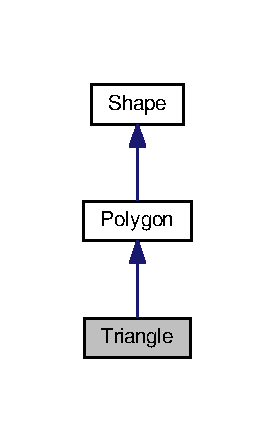
\includegraphics[width=132pt]{class_triangle__inherit__graph}
\end{center}
\end{figure}


Collaboration diagram for Triangle\+:\nopagebreak
\begin{figure}[H]
\begin{center}
\leavevmode
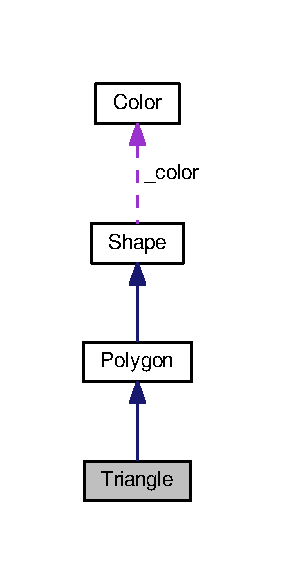
\includegraphics[width=136pt]{class_triangle__coll__graph}
\end{center}
\end{figure}
\subsection*{Public Member Functions}
\begin{DoxyCompactItemize}
\item 
\hyperlink{class_triangle_ab74304b451a87d4c72ece2fe442ca0a7}{Triangle} (const \hyperlink{class_vector2_d}{Vector2D} \&first\+Point, const \hyperlink{class_vector2_d}{Vector2D} \&second\+Point, const \hyperlink{class_vector2_d}{Vector2D} \&third\+Point, const \hyperlink{class_color}{Color} \&color=\hyperlink{class_color_a94697e8c9eb81124c5a7c1439e1e7348}{Color\+::get\+Color}(\char`\"{}black\char`\"{}))
\item 
const \hyperlink{class_vector2_d}{Vector2D} \hyperlink{class_triangle_aa40afc17cb09bf78a863b2e93e5cff45}{get\+First\+Point} () const
\item 
const \hyperlink{class_vector2_d}{Vector2D} \hyperlink{class_triangle_aa92252309b0e6d9ce26a1c9679b7cf19}{get\+Second\+Point} () const
\item 
const \hyperlink{class_vector2_d}{Vector2D} \hyperlink{class_triangle_aa44238e4272fe5a2b9e83974f58f95c6}{get\+Third\+Point} () const
\item 
void \hyperlink{class_triangle_a1fa834143ed718605959a227eba573b3}{draw} (\hyperlink{class_drawing_visitor}{Drawing\+Visitor} $\ast$visitor) const
\item 
\hyperlink{class_triangle_acd8612cc20ffb71e543944c869e4ab81}{operator string} () const
\item 
void \hyperlink{class_triangle_ae9ac3d633172f14d391d290a4467e1d3}{save} (const \hyperlink{class_save_visitor}{Save\+Visitor} $\ast$save\+Visitor, const string \&filename) const
\item 
\hyperlink{class_shape}{Shape} $\ast$ \hyperlink{class_triangle_ac66208b0b633add41b915860f051cf44}{translation} (const \hyperlink{class_vector2_d}{Vector2D} \&translation\+Vector) const
\item 
\hyperlink{class_shape}{Shape} $\ast$ \hyperlink{class_triangle_a45a3a9f74118c99b95c6d8e993773a71}{homothety} (const \hyperlink{class_vector2_d}{Vector2D} \&invariant\+Point, const double \&homothety\+Ratio) const
\item 
\hyperlink{class_shape}{Shape} $\ast$ \hyperlink{class_triangle_a663ca3c6bd7967265849bf1f8c8a464b}{rotation} (const \hyperlink{class_vector2_d}{Vector2D} \&rotation\+Center, const \hyperlink{class_radian_angle}{Radian\+Angle} \&rotation\+Angle) const
\item 
double \hyperlink{class_triangle_a5f7fa9fd678345063e50e3458d943a9b}{get\+Area} () const
\end{DoxyCompactItemize}
\subsection*{Friends}
\begin{DoxyCompactItemize}
\item 
ostream \& \hyperlink{class_triangle_a187347fa130a0bf0bf713db5afe3ee4b}{operator$<$$<$} (ostream \&os, const \hyperlink{class_triangle}{Triangle} \&triangle)
\end{DoxyCompactItemize}
\subsection*{Additional Inherited Members}


\subsection{Detailed Description}
Represent a \hyperlink{class_triangle}{Triangle} It\textquotesingle{}s a \hyperlink{class_shape}{Shape} 

\subsection{Constructor \& Destructor Documentation}
\hypertarget{class_triangle_ab74304b451a87d4c72ece2fe442ca0a7}{}\label{class_triangle_ab74304b451a87d4c72ece2fe442ca0a7} 
\index{Triangle@{Triangle}!Triangle@{Triangle}}
\index{Triangle@{Triangle}!Triangle@{Triangle}}
\subsubsection{\texorpdfstring{Triangle()}{Triangle()}}
{\footnotesize\ttfamily Triangle\+::\+Triangle (\begin{DoxyParamCaption}\item[{const \hyperlink{class_vector2_d}{Vector2D} \&}]{first\+Point,  }\item[{const \hyperlink{class_vector2_d}{Vector2D} \&}]{second\+Point,  }\item[{const \hyperlink{class_vector2_d}{Vector2D} \&}]{third\+Point,  }\item[{const \hyperlink{class_color}{Color} \&}]{color = {\ttfamily \hyperlink{class_color_a94697e8c9eb81124c5a7c1439e1e7348}{Color\+::get\+Color}(\char`\"{}black\char`\"{})} }\end{DoxyParamCaption})}

\hyperlink{class_triangle}{Triangle} constructor 
\begin{DoxyParams}{Parameters}
{\em first\+Point} & the first\+Point of the \hyperlink{class_triangle}{Triangle} \\
\hline
{\em second\+Point} & the second\+Point of the \hyperlink{class_triangle}{Triangle} \\
\hline
{\em third\+Point} & the third\+Point of the \hyperlink{class_triangle}{Triangle} \\
\hline
{\em color} & the color of the \hyperlink{class_triangle}{Triangle} \\
\hline
\end{DoxyParams}


\subsection{Member Function Documentation}
\hypertarget{class_triangle_a1fa834143ed718605959a227eba573b3}{}\label{class_triangle_a1fa834143ed718605959a227eba573b3} 
\index{Triangle@{Triangle}!draw@{draw}}
\index{draw@{draw}!Triangle@{Triangle}}
\subsubsection{\texorpdfstring{draw()}{draw()}}
{\footnotesize\ttfamily void Triangle\+::draw (\begin{DoxyParamCaption}\item[{\hyperlink{class_drawing_visitor}{Drawing\+Visitor} $\ast$}]{visitor }\end{DoxyParamCaption}) const\hspace{0.3cm}{\ttfamily [virtual]}}

Draws the \hyperlink{class_triangle}{Triangle} using a \hyperlink{class_drawing_visitor}{Drawing\+Visitor}. 
\begin{DoxyParams}{Parameters}
{\em visitor} & The \hyperlink{class_drawing_visitor}{Drawing\+Visitor} to use to draw the \hyperlink{class_triangle}{Triangle}. \\
\hline
\end{DoxyParams}


Reimplemented from \hyperlink{class_polygon_a245c526a6a65ea99f5549fe5243006d0}{Polygon}.

\hypertarget{class_triangle_a5f7fa9fd678345063e50e3458d943a9b}{}\label{class_triangle_a5f7fa9fd678345063e50e3458d943a9b} 
\index{Triangle@{Triangle}!get\+Area@{get\+Area}}
\index{get\+Area@{get\+Area}!Triangle@{Triangle}}
\subsubsection{\texorpdfstring{get\+Area()}{getArea()}}
{\footnotesize\ttfamily double Triangle\+::get\+Area (\begin{DoxyParamCaption}{ }\end{DoxyParamCaption}) const\hspace{0.3cm}{\ttfamily [virtual]}}

Returns the area of the \hyperlink{class_triangle}{Triangle}. \begin{DoxyReturn}{Returns}
The area of the \hyperlink{class_triangle}{Triangle}. 
\end{DoxyReturn}


Reimplemented from \hyperlink{class_polygon_ae1ae9dd5e5613f119af3e31488427b01}{Polygon}.

\hypertarget{class_triangle_aa40afc17cb09bf78a863b2e93e5cff45}{}\label{class_triangle_aa40afc17cb09bf78a863b2e93e5cff45} 
\index{Triangle@{Triangle}!get\+First\+Point@{get\+First\+Point}}
\index{get\+First\+Point@{get\+First\+Point}!Triangle@{Triangle}}
\subsubsection{\texorpdfstring{get\+First\+Point()}{getFirstPoint()}}
{\footnotesize\ttfamily const \hyperlink{class_vector2_d}{Vector2D} Triangle\+::get\+First\+Point (\begin{DoxyParamCaption}{ }\end{DoxyParamCaption}) const}

Getter of the first point \begin{DoxyReturn}{Returns}
\hyperlink{class_vector2_d}{Vector2D} The first point 
\end{DoxyReturn}
\hypertarget{class_triangle_aa92252309b0e6d9ce26a1c9679b7cf19}{}\label{class_triangle_aa92252309b0e6d9ce26a1c9679b7cf19} 
\index{Triangle@{Triangle}!get\+Second\+Point@{get\+Second\+Point}}
\index{get\+Second\+Point@{get\+Second\+Point}!Triangle@{Triangle}}
\subsubsection{\texorpdfstring{get\+Second\+Point()}{getSecondPoint()}}
{\footnotesize\ttfamily const \hyperlink{class_vector2_d}{Vector2D} Triangle\+::get\+Second\+Point (\begin{DoxyParamCaption}{ }\end{DoxyParamCaption}) const}

Getter of the second point \begin{DoxyReturn}{Returns}
\hyperlink{class_vector2_d}{Vector2D} The second point 
\end{DoxyReturn}
\hypertarget{class_triangle_aa44238e4272fe5a2b9e83974f58f95c6}{}\label{class_triangle_aa44238e4272fe5a2b9e83974f58f95c6} 
\index{Triangle@{Triangle}!get\+Third\+Point@{get\+Third\+Point}}
\index{get\+Third\+Point@{get\+Third\+Point}!Triangle@{Triangle}}
\subsubsection{\texorpdfstring{get\+Third\+Point()}{getThirdPoint()}}
{\footnotesize\ttfamily const \hyperlink{class_vector2_d}{Vector2D} Triangle\+::get\+Third\+Point (\begin{DoxyParamCaption}{ }\end{DoxyParamCaption}) const}

Getter of the third point \begin{DoxyReturn}{Returns}
\hyperlink{class_vector2_d}{Vector2D} The third point 
\end{DoxyReturn}
\hypertarget{class_triangle_a45a3a9f74118c99b95c6d8e993773a71}{}\label{class_triangle_a45a3a9f74118c99b95c6d8e993773a71} 
\index{Triangle@{Triangle}!homothety@{homothety}}
\index{homothety@{homothety}!Triangle@{Triangle}}
\subsubsection{\texorpdfstring{homothety()}{homothety()}}
{\footnotesize\ttfamily \hyperlink{class_shape}{Shape} $\ast$ Triangle\+::homothety (\begin{DoxyParamCaption}\item[{const \hyperlink{class_vector2_d}{Vector2D} \&}]{invariant\+Point,  }\item[{const double \&}]{homothety\+Ratio }\end{DoxyParamCaption}) const\hspace{0.3cm}{\ttfamily [virtual]}}

Apply an homothety on the \hyperlink{class_triangle}{Triangle}. 
\begin{DoxyParams}{Parameters}
{\em invariant\+Point} & The center of the homothety. \\
\hline
{\em homothety\+Ratio} & The ratio of the homothety. \\
\hline
\end{DoxyParams}
\begin{DoxyReturn}{Returns}
Shape$\ast$ the new triangle after the homotethy 
\end{DoxyReturn}


Reimplemented from \hyperlink{class_polygon_a2b77c7ecbe9ca68664d7f7020181b791}{Polygon}.

\hypertarget{class_triangle_acd8612cc20ffb71e543944c869e4ab81}{}\label{class_triangle_acd8612cc20ffb71e543944c869e4ab81} 
\index{Triangle@{Triangle}!operator string@{operator string}}
\index{operator string@{operator string}!Triangle@{Triangle}}
\subsubsection{\texorpdfstring{operator string()}{operator string()}}
{\footnotesize\ttfamily Triangle\+::operator string (\begin{DoxyParamCaption}{ }\end{DoxyParamCaption}) const\hspace{0.3cm}{\ttfamily [virtual]}}

Returns a string that represents the \hyperlink{class_triangle}{Triangle}. \begin{DoxyReturn}{Returns}
The string representing the \hyperlink{class_triangle}{Triangle}. 
\end{DoxyReturn}


Reimplemented from \hyperlink{class_polygon_a41c29b75f2463646af0f7bd604a4853d}{Polygon}.

\hypertarget{class_triangle_a663ca3c6bd7967265849bf1f8c8a464b}{}\label{class_triangle_a663ca3c6bd7967265849bf1f8c8a464b} 
\index{Triangle@{Triangle}!rotation@{rotation}}
\index{rotation@{rotation}!Triangle@{Triangle}}
\subsubsection{\texorpdfstring{rotation()}{rotation()}}
{\footnotesize\ttfamily \hyperlink{class_shape}{Shape} $\ast$ Triangle\+::rotation (\begin{DoxyParamCaption}\item[{const \hyperlink{class_vector2_d}{Vector2D} \&}]{rotation\+Center,  }\item[{const \hyperlink{class_radian_angle}{Radian\+Angle} \&}]{rotation\+Angle }\end{DoxyParamCaption}) const\hspace{0.3cm}{\ttfamily [virtual]}}

Rotates the \hyperlink{class_triangle}{Triangle}. 
\begin{DoxyParams}{Parameters}
{\em rotation\+Center} & The center of the rotation. \\
\hline
{\em rotation\+Angle} & The angle of the rotation. \\
\hline
\end{DoxyParams}
\begin{DoxyReturn}{Returns}
Shape$\ast$ the new \hyperlink{class_triangle}{Triangle} after the rotation 
\end{DoxyReturn}


Reimplemented from \hyperlink{class_polygon_a5a453f01700f97ca98b0487cd670b194}{Polygon}.

\hypertarget{class_triangle_ae9ac3d633172f14d391d290a4467e1d3}{}\label{class_triangle_ae9ac3d633172f14d391d290a4467e1d3} 
\index{Triangle@{Triangle}!save@{save}}
\index{save@{save}!Triangle@{Triangle}}
\subsubsection{\texorpdfstring{save()}{save()}}
{\footnotesize\ttfamily void Triangle\+::save (\begin{DoxyParamCaption}\item[{const \hyperlink{class_save_visitor}{Save\+Visitor} $\ast$}]{save\+Visitor,  }\item[{const string \&}]{filename }\end{DoxyParamCaption}) const\hspace{0.3cm}{\ttfamily [virtual]}}

Saves the \hyperlink{class_triangle}{Triangle}. 
\begin{DoxyParams}{Parameters}
{\em save\+Visitor} & The \hyperlink{class_save_visitor}{Save\+Visitor} to use to save the \hyperlink{class_triangle}{Triangle}. \\
\hline
\end{DoxyParams}


Reimplemented from \hyperlink{class_polygon_ad9adb867821b71e1aa8130dccbc9b37f}{Polygon}.

\hypertarget{class_triangle_ac66208b0b633add41b915860f051cf44}{}\label{class_triangle_ac66208b0b633add41b915860f051cf44} 
\index{Triangle@{Triangle}!translation@{translation}}
\index{translation@{translation}!Triangle@{Triangle}}
\subsubsection{\texorpdfstring{translation()}{translation()}}
{\footnotesize\ttfamily \hyperlink{class_shape}{Shape} $\ast$ Triangle\+::translation (\begin{DoxyParamCaption}\item[{const \hyperlink{class_vector2_d}{Vector2D} \&}]{translation\+Vector }\end{DoxyParamCaption}) const\hspace{0.3cm}{\ttfamily [virtual]}}

Translate the \hyperlink{class_triangle}{Triangle} using a translation vector. 
\begin{DoxyParams}{Parameters}
{\em translation\+Vector} & The translation vector to use for the translation. \\
\hline
\end{DoxyParams}
\begin{DoxyReturn}{Returns}
Shape$\ast$ the new \hyperlink{class_triangle}{Triangle} after the translation 
\end{DoxyReturn}


Reimplemented from \hyperlink{class_polygon_ae828addfa5cffab547bcb16db1f275be}{Polygon}.



\subsection{Friends And Related Function Documentation}
\hypertarget{class_triangle_a187347fa130a0bf0bf713db5afe3ee4b}{}\label{class_triangle_a187347fa130a0bf0bf713db5afe3ee4b} 
\index{Triangle@{Triangle}!operator$<$$<$@{operator$<$$<$}}
\index{operator$<$$<$@{operator$<$$<$}!Triangle@{Triangle}}
\subsubsection{\texorpdfstring{operator$<$$<$}{operator<<}}
{\footnotesize\ttfamily ostream\& operator$<$$<$ (\begin{DoxyParamCaption}\item[{ostream \&}]{os,  }\item[{const \hyperlink{class_triangle}{Triangle} \&}]{triangle }\end{DoxyParamCaption})\hspace{0.3cm}{\ttfamily [friend]}}



The documentation for this class was generated from the following files\+:\begin{DoxyCompactItemize}
\item 
src/\+Shape/\hyperlink{_triangle_8hpp}{Triangle.\+hpp}\item 
src/\+Shape/\hyperlink{_triangle_8cpp}{Triangle.\+cpp}\end{DoxyCompactItemize}

\hypertarget{class_triangle_creator}{}\section{Triangle\+Creator Class Reference}
\label{class_triangle_creator}\index{Triangle\+Creator@{Triangle\+Creator}}


{\ttfamily \#include $<$Triangle\+Creator.\+hpp$>$}



Inheritance diagram for Triangle\+Creator\+:\nopagebreak
\begin{figure}[H]
\begin{center}
\leavevmode
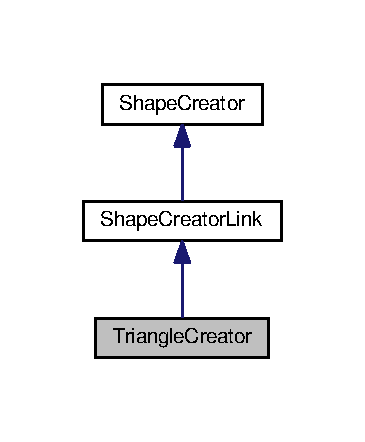
\includegraphics[width=175pt]{class_triangle_creator__inherit__graph}
\end{center}
\end{figure}


Collaboration diagram for Triangle\+Creator\+:\nopagebreak
\begin{figure}[H]
\begin{center}
\leavevmode
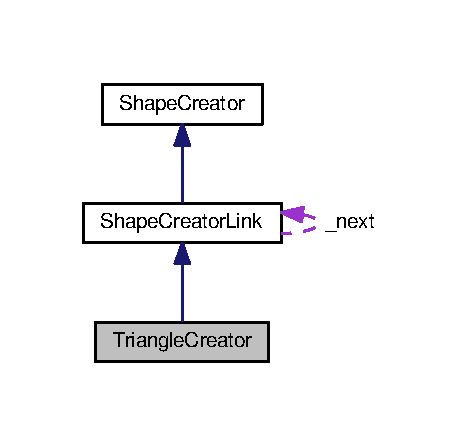
\includegraphics[width=221pt]{class_triangle_creator__coll__graph}
\end{center}
\end{figure}
\subsection*{Public Member Functions}
\begin{DoxyCompactItemize}
\item 
\hyperlink{class_triangle_creator_a89e29090c1f072d81562e448a98a138d}{Triangle\+Creator} (\hyperlink{class_shape_creator_link}{Shape\+Creator\+Link} $\ast$next)
\item 
virtual \hyperlink{class_shape}{Shape} $\ast$ \hyperlink{class_triangle_creator_a8698d657d98a7be93aeaf86b2434bbb3}{create\+Shape\+Spe} (const string \&shape\+String) const
\end{DoxyCompactItemize}
\subsection*{Additional Inherited Members}


\subsection{Detailed Description}
Class \hyperlink{class_triangle_creator}{Triangle\+Creator} Link of the C\+OR for build \hyperlink{class_triangle}{Triangle} 

\subsection{Constructor \& Destructor Documentation}
\hypertarget{class_triangle_creator_a89e29090c1f072d81562e448a98a138d}{}\label{class_triangle_creator_a89e29090c1f072d81562e448a98a138d} 
\index{Triangle\+Creator@{Triangle\+Creator}!Triangle\+Creator@{Triangle\+Creator}}
\index{Triangle\+Creator@{Triangle\+Creator}!Triangle\+Creator@{Triangle\+Creator}}
\subsubsection{\texorpdfstring{Triangle\+Creator()}{TriangleCreator()}}
{\footnotesize\ttfamily Triangle\+Creator\+::\+Triangle\+Creator (\begin{DoxyParamCaption}\item[{\hyperlink{class_shape_creator_link}{Shape\+Creator\+Link} $\ast$}]{next }\end{DoxyParamCaption})}

Constructor of \hyperlink{class_triangle_creator}{Triangle\+Creator} 
\begin{DoxyParams}{Parameters}
{\em next} & The next \hyperlink{class_shape_creator_link}{Shape\+Creator\+Link} if this one fails \\
\hline
\end{DoxyParams}


\subsection{Member Function Documentation}
\hypertarget{class_triangle_creator_a8698d657d98a7be93aeaf86b2434bbb3}{}\label{class_triangle_creator_a8698d657d98a7be93aeaf86b2434bbb3} 
\index{Triangle\+Creator@{Triangle\+Creator}!create\+Shape\+Spe@{create\+Shape\+Spe}}
\index{create\+Shape\+Spe@{create\+Shape\+Spe}!Triangle\+Creator@{Triangle\+Creator}}
\subsubsection{\texorpdfstring{create\+Shape\+Spe()}{createShapeSpe()}}
{\footnotesize\ttfamily \hyperlink{class_shape}{Shape} $\ast$ Triangle\+Creator\+::create\+Shape\+Spe (\begin{DoxyParamCaption}\item[{const string \&}]{shape\+String }\end{DoxyParamCaption}) const\hspace{0.3cm}{\ttfamily [virtual]}}

Try to create a \hyperlink{class_triangle}{Triangle} with the string 
\begin{DoxyParams}{Parameters}
{\em shape\+String} & the string with informations of the shape \\
\hline
\end{DoxyParams}
\begin{DoxyReturn}{Returns}
The Shape$\ast$ wich were created 
\end{DoxyReturn}


Implements \hyperlink{class_shape_creator_link_a036ecc845946d23b36335e9077308bcf}{Shape\+Creator\+Link}.



The documentation for this class was generated from the following files\+:\begin{DoxyCompactItemize}
\item 
src/\+Loader/\hyperlink{_triangle_creator_8hpp}{Triangle\+Creator.\+hpp}\item 
src/\+Loader/\hyperlink{_triangle_creator_8cpp}{Triangle\+Creator.\+cpp}\end{DoxyCompactItemize}

\hypertarget{class_utils_exception}{}\section{Utils\+Exception Class Reference}
\label{class_utils_exception}\index{Utils\+Exception@{Utils\+Exception}}


{\ttfamily \#include $<$Utils\+Exception.\+hpp$>$}

\subsection*{Public Member Functions}
\begin{DoxyCompactItemize}
\item 
\hyperlink{class_utils_exception_ab8cad43c55b3ce4a62e32b85c1c46491}{Utils\+Exception} (const string \&message)
\end{DoxyCompactItemize}
\subsection*{Friends}
\begin{DoxyCompactItemize}
\item 
ostream \& \hyperlink{class_utils_exception_a6ebd1d5ff627152beaa743b43fc2f9d3}{operator$<$$<$} (ostream \&os, const \hyperlink{class_utils_exception}{Utils\+Exception} \&utils\+Exception)
\end{DoxyCompactItemize}


\subsection{Detailed Description}
Class for hander all utils exceptions 

\subsection{Constructor \& Destructor Documentation}
\hypertarget{class_utils_exception_ab8cad43c55b3ce4a62e32b85c1c46491}{}\label{class_utils_exception_ab8cad43c55b3ce4a62e32b85c1c46491} 
\index{Utils\+Exception@{Utils\+Exception}!Utils\+Exception@{Utils\+Exception}}
\index{Utils\+Exception@{Utils\+Exception}!Utils\+Exception@{Utils\+Exception}}
\subsubsection{\texorpdfstring{Utils\+Exception()}{UtilsException()}}
{\footnotesize\ttfamily Utils\+Exception\+::\+Utils\+Exception (\begin{DoxyParamCaption}\item[{const string \&}]{message }\end{DoxyParamCaption})}

Constructor of \hyperlink{class_utils_exception}{Utils\+Exception} 
\begin{DoxyParams}{Parameters}
{\em message} & the message to throw \\
\hline
\end{DoxyParams}


\subsection{Friends And Related Function Documentation}
\hypertarget{class_utils_exception_a6ebd1d5ff627152beaa743b43fc2f9d3}{}\label{class_utils_exception_a6ebd1d5ff627152beaa743b43fc2f9d3} 
\index{Utils\+Exception@{Utils\+Exception}!operator$<$$<$@{operator$<$$<$}}
\index{operator$<$$<$@{operator$<$$<$}!Utils\+Exception@{Utils\+Exception}}
\subsubsection{\texorpdfstring{operator$<$$<$}{operator<<}}
{\footnotesize\ttfamily ostream\& operator$<$$<$ (\begin{DoxyParamCaption}\item[{ostream \&}]{os,  }\item[{const \hyperlink{class_utils_exception}{Utils\+Exception} \&}]{utils\+Exception }\end{DoxyParamCaption})\hspace{0.3cm}{\ttfamily [friend]}}

Sends a string of excpetion to a stream 
\begin{DoxyParams}{Parameters}
{\em os} & ostream \\
\hline
{\em utils\+Exception} & utils\+Exception have to print \\
\hline
\end{DoxyParams}
\begin{DoxyReturn}{Returns}
ostream to send to the output 
\end{DoxyReturn}


The documentation for this class was generated from the following files\+:\begin{DoxyCompactItemize}
\item 
src/\+Utils/\hyperlink{_utils_exception_8hpp}{Utils\+Exception.\+hpp}\item 
src/\+Utils/\hyperlink{_utils_exception_8cpp}{Utils\+Exception.\+cpp}\end{DoxyCompactItemize}

\hypertarget{class_vector2_d}{}\section{Vector2D Class Reference}
\label{class_vector2_d}\index{Vector2D@{Vector2D}}


{\ttfamily \#include $<$Vector2\+D.\+hpp$>$}

\subsection*{Public Member Functions}
\begin{DoxyCompactItemize}
\item 
\hyperlink{class_vector2_d_affaf87a7d9ce6c6566c8fe0fe000dfae}{Vector2D} (const double \&x=0, const double \&y=0)
\item 
virtual \hyperlink{class_vector2_d_ac0f819527d3966874c4c9bb72ab9f67e}{$\sim$\+Vector2D} ()
\item 
double \hyperlink{class_vector2_d_a5957acade3579baa63807d625316d557}{getX} () const
\item 
double \hyperlink{class_vector2_d_a4ae19b97cfbc35850b9717a25ea83104}{getY} () const
\item 
void \hyperlink{class_vector2_d_aefc6ba44c9fbf5f877fbd70460a4dcaf}{setX} (double x)
\item 
void \hyperlink{class_vector2_d_a2f68870e57beb7116b457a143fee4362}{setY} (double y)
\item 
\hyperlink{class_vector2_d_aa5286e82a3c62dd101dd7203943bb0f0}{operator string} () const
\item 
const \hyperlink{class_vector2_d}{Vector2D} \hyperlink{class_vector2_d_a068660b7b836163e6a417c8fb283022b}{operator+} (const \hyperlink{class_vector2_d}{Vector2D} \&rhv) const
\item 
const \hyperlink{class_vector2_d}{Vector2D} \& \hyperlink{class_vector2_d_a5e4dc932362899c8e7bf8b0caea1c9a9}{operator+=} (const \hyperlink{class_vector2_d}{Vector2D} \&rhs)
\item 
const \hyperlink{class_vector2_d}{Vector2D} \hyperlink{class_vector2_d_a4931b15799ccc2432d472fff3ee76e39}{operator$\ast$} (const double \&a) const
\item 
const \hyperlink{class_vector2_d}{Vector2D} \& \hyperlink{class_vector2_d_a9ec785cca2a48d62596dfdbfa0546267}{operator$\ast$=} (const double \&a)
\item 
const \hyperlink{class_vector2_d}{Vector2D} \hyperlink{class_vector2_d_a03bb71dddee9f2d265410b932711b9a4}{operator-\/} () const
\item 
const \hyperlink{class_vector2_d}{Vector2D} \hyperlink{class_vector2_d_a107f6955e56db7e2f0f8e86e6a4a4be2}{operator-\/} (const \hyperlink{class_vector2_d}{Vector2D} \&rhv) const
\item 
const \hyperlink{class_vector2_d}{Vector2D} \& \hyperlink{class_vector2_d_a39e1e309b40f2b3df02d26911e4637cc}{operator-\/=} (const \hyperlink{class_vector2_d}{Vector2D} \&rhs)
\item 
void \hyperlink{class_vector2_d_a86c7035a75207b3666a688eb9f4f6170}{translation} (const \hyperlink{class_vector2_d}{Vector2D} \&translation\+Vector)
\item 
void \hyperlink{class_vector2_d_ac8556496b88bf5a0928615822457b7b3}{homothety} (const \hyperlink{class_vector2_d}{Vector2D} \&invariant\+Point, const double \&homothety\+Ratio)
\item 
void \hyperlink{class_vector2_d_ad6604a58165c7144f87b8f555d248dde}{rotation} (const \hyperlink{class_vector2_d}{Vector2D} \&rotation\+Center, const \hyperlink{class_radian_angle}{Radian\+Angle} \&rotation\+Angle)
\end{DoxyCompactItemize}
\subsection*{Friends}
\begin{DoxyCompactItemize}
\item 
ostream \& \hyperlink{class_vector2_d_a947884ffef441f605f61b9bb1a2dab13}{operator$<$$<$} (ostream \&os, const \hyperlink{class_vector2_d}{Vector2D} \&vector)
\end{DoxyCompactItemize}


\subsection{Detailed Description}
Class represents a point in space 

\subsection{Constructor \& Destructor Documentation}
\hypertarget{class_vector2_d_affaf87a7d9ce6c6566c8fe0fe000dfae}{}\label{class_vector2_d_affaf87a7d9ce6c6566c8fe0fe000dfae} 
\index{Vector2D@{Vector2D}!Vector2D@{Vector2D}}
\index{Vector2D@{Vector2D}!Vector2D@{Vector2D}}
\subsubsection{\texorpdfstring{Vector2\+D()}{Vector2D()}}
{\footnotesize\ttfamily Vector2\+D\+::\+Vector2D (\begin{DoxyParamCaption}\item[{const double \&}]{x = {\ttfamily 0},  }\item[{const double \&}]{y = {\ttfamily 0} }\end{DoxyParamCaption})}

Constructor 
\begin{DoxyParams}{Parameters}
{\em x} & double for the abscissa, 0 default \\
\hline
{\em y} & double for the ordonate, 0 default \\
\hline
\end{DoxyParams}
\hypertarget{class_vector2_d_ac0f819527d3966874c4c9bb72ab9f67e}{}\label{class_vector2_d_ac0f819527d3966874c4c9bb72ab9f67e} 
\index{Vector2D@{Vector2D}!````~Vector2D@{$\sim$\+Vector2D}}
\index{````~Vector2D@{$\sim$\+Vector2D}!Vector2D@{Vector2D}}
\subsubsection{\texorpdfstring{$\sim$\+Vector2\+D()}{~Vector2D()}}
{\footnotesize\ttfamily Vector2\+D\+::$\sim$\+Vector2D (\begin{DoxyParamCaption}{ }\end{DoxyParamCaption})\hspace{0.3cm}{\ttfamily [virtual]}}

Destructor 

\subsection{Member Function Documentation}
\hypertarget{class_vector2_d_a5957acade3579baa63807d625316d557}{}\label{class_vector2_d_a5957acade3579baa63807d625316d557} 
\index{Vector2D@{Vector2D}!getX@{getX}}
\index{getX@{getX}!Vector2D@{Vector2D}}
\subsubsection{\texorpdfstring{get\+X()}{getX()}}
{\footnotesize\ttfamily double Vector2\+D\+::getX (\begin{DoxyParamCaption}{ }\end{DoxyParamCaption}) const\hspace{0.3cm}{\ttfamily [inline]}}

Gets \+\_\+x (abscissa) \hypertarget{class_vector2_d_a4ae19b97cfbc35850b9717a25ea83104}{}\label{class_vector2_d_a4ae19b97cfbc35850b9717a25ea83104} 
\index{Vector2D@{Vector2D}!getY@{getY}}
\index{getY@{getY}!Vector2D@{Vector2D}}
\subsubsection{\texorpdfstring{get\+Y()}{getY()}}
{\footnotesize\ttfamily double Vector2\+D\+::getY (\begin{DoxyParamCaption}{ }\end{DoxyParamCaption}) const\hspace{0.3cm}{\ttfamily [inline]}}

Gets \+\_\+y (ordonate) \hypertarget{class_vector2_d_ac8556496b88bf5a0928615822457b7b3}{}\label{class_vector2_d_ac8556496b88bf5a0928615822457b7b3} 
\index{Vector2D@{Vector2D}!homothety@{homothety}}
\index{homothety@{homothety}!Vector2D@{Vector2D}}
\subsubsection{\texorpdfstring{homothety()}{homothety()}}
{\footnotesize\ttfamily void Vector2\+D\+::homothety (\begin{DoxyParamCaption}\item[{const \hyperlink{class_vector2_d}{Vector2D} \&}]{invariant\+Point,  }\item[{const double \&}]{homothety\+Ratio }\end{DoxyParamCaption})}

Make homothety of a vector2D 
\begin{DoxyParams}{Parameters}
{\em invariant\+Point} & \\
\hline
{\em homothety\+Ratio} & \\
\hline
\end{DoxyParams}
\hypertarget{class_vector2_d_aa5286e82a3c62dd101dd7203943bb0f0}{}\label{class_vector2_d_aa5286e82a3c62dd101dd7203943bb0f0} 
\index{Vector2D@{Vector2D}!operator string@{operator string}}
\index{operator string@{operator string}!Vector2D@{Vector2D}}
\subsubsection{\texorpdfstring{operator string()}{operator string()}}
{\footnotesize\ttfamily Vector2\+D\+::operator string (\begin{DoxyParamCaption}{ }\end{DoxyParamCaption}) const}

Operator cast to string \hypertarget{class_vector2_d_a4931b15799ccc2432d472fff3ee76e39}{}\label{class_vector2_d_a4931b15799ccc2432d472fff3ee76e39} 
\index{Vector2D@{Vector2D}!operator$\ast$@{operator$\ast$}}
\index{operator$\ast$@{operator$\ast$}!Vector2D@{Vector2D}}
\subsubsection{\texorpdfstring{operator$\ast$()}{operator*()}}
{\footnotesize\ttfamily const \hyperlink{class_vector2_d}{Vector2D} Vector2\+D\+::operator$\ast$ (\begin{DoxyParamCaption}\item[{const double \&}]{a }\end{DoxyParamCaption}) const}

Allows to multiply a vector by a constant 
\begin{DoxyParams}{Parameters}
{\em a} & double to multiply \\
\hline
\end{DoxyParams}
\begin{DoxyReturn}{Returns}
\hyperlink{class_vector2_d}{Vector2D} which is the result of product 
\end{DoxyReturn}
\hypertarget{class_vector2_d_a9ec785cca2a48d62596dfdbfa0546267}{}\label{class_vector2_d_a9ec785cca2a48d62596dfdbfa0546267} 
\index{Vector2D@{Vector2D}!operator$\ast$=@{operator$\ast$=}}
\index{operator$\ast$=@{operator$\ast$=}!Vector2D@{Vector2D}}
\subsubsection{\texorpdfstring{operator$\ast$=()}{operator*=()}}
{\footnotesize\ttfamily const \hyperlink{class_vector2_d}{Vector2D} \& Vector2\+D\+::operator$\ast$= (\begin{DoxyParamCaption}\item[{const double \&}]{a }\end{DoxyParamCaption})}

\hypertarget{class_vector2_d_a068660b7b836163e6a417c8fb283022b}{}\label{class_vector2_d_a068660b7b836163e6a417c8fb283022b} 
\index{Vector2D@{Vector2D}!operator+@{operator+}}
\index{operator+@{operator+}!Vector2D@{Vector2D}}
\subsubsection{\texorpdfstring{operator+()}{operator+()}}
{\footnotesize\ttfamily const \hyperlink{class_vector2_d}{Vector2D} Vector2\+D\+::operator+ (\begin{DoxyParamCaption}\item[{const \hyperlink{class_vector2_d}{Vector2D} \&}]{rhv }\end{DoxyParamCaption}) const}

Allows to add two vectors 
\begin{DoxyParams}{Parameters}
{\em rhv} & vector to add \\
\hline
\end{DoxyParams}
\begin{DoxyReturn}{Returns}
\hyperlink{class_vector2_d}{Vector2D} which is the result of addition 
\end{DoxyReturn}
\hypertarget{class_vector2_d_a5e4dc932362899c8e7bf8b0caea1c9a9}{}\label{class_vector2_d_a5e4dc932362899c8e7bf8b0caea1c9a9} 
\index{Vector2D@{Vector2D}!operator+=@{operator+=}}
\index{operator+=@{operator+=}!Vector2D@{Vector2D}}
\subsubsection{\texorpdfstring{operator+=()}{operator+=()}}
{\footnotesize\ttfamily const \hyperlink{class_vector2_d}{Vector2D} \& Vector2\+D\+::operator+= (\begin{DoxyParamCaption}\item[{const \hyperlink{class_vector2_d}{Vector2D} \&}]{rhs }\end{DoxyParamCaption})}

\hypertarget{class_vector2_d_a03bb71dddee9f2d265410b932711b9a4}{}\label{class_vector2_d_a03bb71dddee9f2d265410b932711b9a4} 
\index{Vector2D@{Vector2D}!operator-\/@{operator-\/}}
\index{operator-\/@{operator-\/}!Vector2D@{Vector2D}}
\subsubsection{\texorpdfstring{operator-\/()}{operator-()}\hspace{0.1cm}{\footnotesize\ttfamily [1/2]}}
{\footnotesize\ttfamily const \hyperlink{class_vector2_d}{Vector2D} Vector2\+D\+::operator-\/ (\begin{DoxyParamCaption}{ }\end{DoxyParamCaption}) const}

Gets the opposite of a vector \begin{DoxyReturn}{Returns}
\hyperlink{class_vector2_d}{Vector2D} 
\end{DoxyReturn}
\hypertarget{class_vector2_d_a107f6955e56db7e2f0f8e86e6a4a4be2}{}\label{class_vector2_d_a107f6955e56db7e2f0f8e86e6a4a4be2} 
\index{Vector2D@{Vector2D}!operator-\/@{operator-\/}}
\index{operator-\/@{operator-\/}!Vector2D@{Vector2D}}
\subsubsection{\texorpdfstring{operator-\/()}{operator-()}\hspace{0.1cm}{\footnotesize\ttfamily [2/2]}}
{\footnotesize\ttfamily const \hyperlink{class_vector2_d}{Vector2D} Vector2\+D\+::operator-\/ (\begin{DoxyParamCaption}\item[{const \hyperlink{class_vector2_d}{Vector2D} \&}]{rhv }\end{DoxyParamCaption}) const}

Allows to substract two vectors 
\begin{DoxyParams}{Parameters}
{\em rhv} & vector to sub \\
\hline
\end{DoxyParams}
\begin{DoxyReturn}{Returns}
\hyperlink{class_vector2_d}{Vector2D} which is the result of substraction 
\end{DoxyReturn}
\hypertarget{class_vector2_d_a39e1e309b40f2b3df02d26911e4637cc}{}\label{class_vector2_d_a39e1e309b40f2b3df02d26911e4637cc} 
\index{Vector2D@{Vector2D}!operator-\/=@{operator-\/=}}
\index{operator-\/=@{operator-\/=}!Vector2D@{Vector2D}}
\subsubsection{\texorpdfstring{operator-\/=()}{operator-=()}}
{\footnotesize\ttfamily const \hyperlink{class_vector2_d}{Vector2D} \& Vector2\+D\+::operator-\/= (\begin{DoxyParamCaption}\item[{const \hyperlink{class_vector2_d}{Vector2D} \&}]{rhs }\end{DoxyParamCaption})}

\hypertarget{class_vector2_d_ad6604a58165c7144f87b8f555d248dde}{}\label{class_vector2_d_ad6604a58165c7144f87b8f555d248dde} 
\index{Vector2D@{Vector2D}!rotation@{rotation}}
\index{rotation@{rotation}!Vector2D@{Vector2D}}
\subsubsection{\texorpdfstring{rotation()}{rotation()}}
{\footnotesize\ttfamily const \hyperlink{class_vector2_d}{Vector2D} Vector2\+D\+::rotation (\begin{DoxyParamCaption}\item[{const \hyperlink{class_vector2_d}{Vector2D} \&}]{rotation\+Center,  }\item[{const \hyperlink{class_radian_angle}{Radian\+Angle} \&}]{rotation\+Angle }\end{DoxyParamCaption})}

Make rotation of a vector2D 
\begin{DoxyParams}{Parameters}
{\em rotation\+Center} & \\
\hline
{\em rotation\+Angle} & \\
\hline
\end{DoxyParams}
\hypertarget{class_vector2_d_aefc6ba44c9fbf5f877fbd70460a4dcaf}{}\label{class_vector2_d_aefc6ba44c9fbf5f877fbd70460a4dcaf} 
\index{Vector2D@{Vector2D}!setX@{setX}}
\index{setX@{setX}!Vector2D@{Vector2D}}
\subsubsection{\texorpdfstring{set\+X()}{setX()}}
{\footnotesize\ttfamily void Vector2\+D\+::setX (\begin{DoxyParamCaption}\item[{double}]{x }\end{DoxyParamCaption})\hspace{0.3cm}{\ttfamily [inline]}}

\hypertarget{class_vector2_d_a2f68870e57beb7116b457a143fee4362}{}\label{class_vector2_d_a2f68870e57beb7116b457a143fee4362} 
\index{Vector2D@{Vector2D}!setY@{setY}}
\index{setY@{setY}!Vector2D@{Vector2D}}
\subsubsection{\texorpdfstring{set\+Y()}{setY()}}
{\footnotesize\ttfamily void Vector2\+D\+::setY (\begin{DoxyParamCaption}\item[{double}]{y }\end{DoxyParamCaption})\hspace{0.3cm}{\ttfamily [inline]}}

\hypertarget{class_vector2_d_a86c7035a75207b3666a688eb9f4f6170}{}\label{class_vector2_d_a86c7035a75207b3666a688eb9f4f6170} 
\index{Vector2D@{Vector2D}!translation@{translation}}
\index{translation@{translation}!Vector2D@{Vector2D}}
\subsubsection{\texorpdfstring{translation()}{translation()}}
{\footnotesize\ttfamily void Vector2\+D\+::translation (\begin{DoxyParamCaption}\item[{const \hyperlink{class_vector2_d}{Vector2D} \&}]{translation\+Vector }\end{DoxyParamCaption})}

Make translation of a vector2D 
\begin{DoxyParams}{Parameters}
{\em translation\+Vector} & \\
\hline
\end{DoxyParams}


\subsection{Friends And Related Function Documentation}
\hypertarget{class_vector2_d_a947884ffef441f605f61b9bb1a2dab13}{}\label{class_vector2_d_a947884ffef441f605f61b9bb1a2dab13} 
\index{Vector2D@{Vector2D}!operator$<$$<$@{operator$<$$<$}}
\index{operator$<$$<$@{operator$<$$<$}!Vector2D@{Vector2D}}
\subsubsection{\texorpdfstring{operator$<$$<$}{operator<<}}
{\footnotesize\ttfamily ostream\& operator$<$$<$ (\begin{DoxyParamCaption}\item[{ostream \&}]{os,  }\item[{const \hyperlink{class_vector2_d}{Vector2D} \&}]{vector }\end{DoxyParamCaption})\hspace{0.3cm}{\ttfamily [friend]}}

Sends a string of vector to a stream 
\begin{DoxyParams}{Parameters}
{\em os} & ostream \\
\hline
{\em vector} & vector have to print \\
\hline
\end{DoxyParams}
\begin{DoxyReturn}{Returns}
ostream to send to the output 
\end{DoxyReturn}


The documentation for this class was generated from the following files\+:\begin{DoxyCompactItemize}
\item 
src/\+Geometry/\hyperlink{_vector2_d_8hpp}{Vector2\+D.\+hpp}\item 
src/\+Geometry/\hyperlink{_vector2_d_8cpp}{Vector2\+D.\+cpp}\end{DoxyCompactItemize}

\chapter{File Documentation}
\hypertarget{_geometry_exception_8cpp}{}\section{src/\+Geometry/\+Geometry\+Exception.cpp File Reference}
\label{_geometry_exception_8cpp}\index{src/\+Geometry/\+Geometry\+Exception.\+cpp@{src/\+Geometry/\+Geometry\+Exception.\+cpp}}
{\ttfamily \#include \char`\"{}Geometry\+Exception.\+hpp\char`\"{}}\newline
{\ttfamily \#include $<$iostream$>$}\newline
Include dependency graph for Geometry\+Exception.\+cpp\+:\nopagebreak
\begin{figure}[H]
\begin{center}
\leavevmode
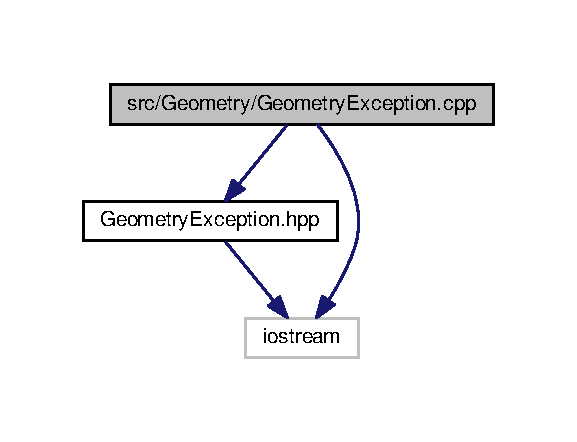
\includegraphics[width=277pt]{_geometry_exception_8cpp__incl}
\end{center}
\end{figure}
\subsection*{Functions}
\begin{DoxyCompactItemize}
\item 
ostream \& \hyperlink{_geometry_exception_8cpp_a1a0e9b6dde275e9a72dd6538ab4a7b73}{operator$<$$<$} (ostream \&os, const \hyperlink{class_geometry_exception}{Geometry\+Exception} \&geometry\+Exception)
\end{DoxyCompactItemize}


\subsection{Function Documentation}
\hypertarget{_geometry_exception_8cpp_a1a0e9b6dde275e9a72dd6538ab4a7b73}{}\label{_geometry_exception_8cpp_a1a0e9b6dde275e9a72dd6538ab4a7b73} 
\index{Geometry\+Exception.\+cpp@{Geometry\+Exception.\+cpp}!operator$<$$<$@{operator$<$$<$}}
\index{operator$<$$<$@{operator$<$$<$}!Geometry\+Exception.\+cpp@{Geometry\+Exception.\+cpp}}
\subsubsection{\texorpdfstring{operator$<$$<$()}{operator<<()}}
{\footnotesize\ttfamily ostream\& operator$<$$<$ (\begin{DoxyParamCaption}\item[{ostream \&}]{os,  }\item[{const \hyperlink{class_geometry_exception}{Geometry\+Exception} \&}]{geometry\+Exception }\end{DoxyParamCaption})}

Sends a string of excpetion to a stream 
\begin{DoxyParams}{Parameters}
{\em os} & ostream \\
\hline
{\em geometry\+Exception} & \hyperlink{class_geometry_exception}{Geometry\+Exception} have to print \\
\hline
\end{DoxyParams}
\begin{DoxyReturn}{Returns}
ostream to send to the output 
\end{DoxyReturn}

\hypertarget{_geometry_exception_8hpp}{}\section{src/\+Geometry/\+Geometry\+Exception.hpp File Reference}
\label{_geometry_exception_8hpp}\index{src/\+Geometry/\+Geometry\+Exception.\+hpp@{src/\+Geometry/\+Geometry\+Exception.\+hpp}}
{\ttfamily \#include $<$iostream$>$}\newline
Include dependency graph for Geometry\+Exception.\+hpp\+:\nopagebreak
\begin{figure}[H]
\begin{center}
\leavevmode
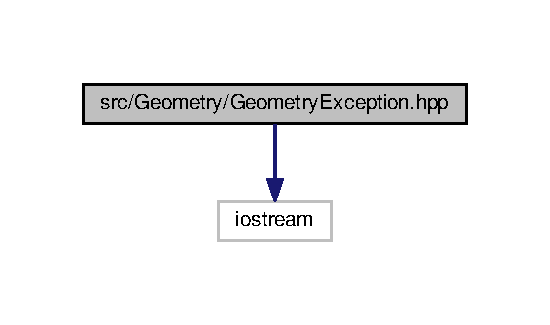
\includegraphics[width=264pt]{_geometry_exception_8hpp__incl}
\end{center}
\end{figure}
This graph shows which files directly or indirectly include this file\+:\nopagebreak
\begin{figure}[H]
\begin{center}
\leavevmode
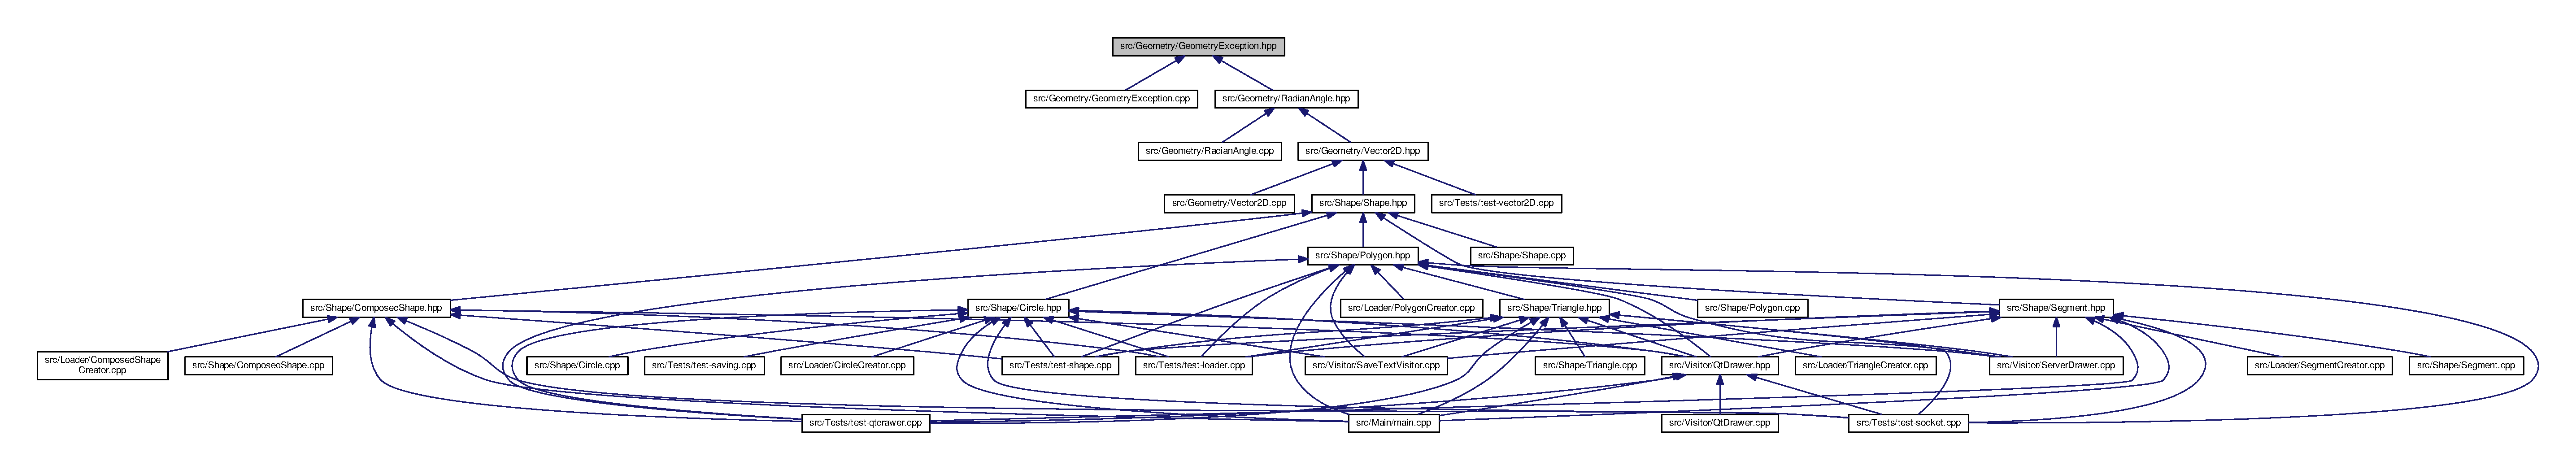
\includegraphics[width=350pt]{_geometry_exception_8hpp__dep__incl}
\end{center}
\end{figure}
\subsection*{Classes}
\begin{DoxyCompactItemize}
\item 
class \hyperlink{class_geometry_exception}{Geometry\+Exception}
\end{DoxyCompactItemize}
\subsection*{Functions}
\begin{DoxyCompactItemize}
\item 
ostream \& \hyperlink{_geometry_exception_8hpp_a1a0e9b6dde275e9a72dd6538ab4a7b73}{operator$<$$<$} (ostream \&os, const \hyperlink{class_geometry_exception}{Geometry\+Exception} \&geometry\+Exception)
\end{DoxyCompactItemize}


\subsection{Function Documentation}
\hypertarget{_geometry_exception_8hpp_a1a0e9b6dde275e9a72dd6538ab4a7b73}{}\label{_geometry_exception_8hpp_a1a0e9b6dde275e9a72dd6538ab4a7b73} 
\index{Geometry\+Exception.\+hpp@{Geometry\+Exception.\+hpp}!operator$<$$<$@{operator$<$$<$}}
\index{operator$<$$<$@{operator$<$$<$}!Geometry\+Exception.\+hpp@{Geometry\+Exception.\+hpp}}
\subsubsection{\texorpdfstring{operator$<$$<$()}{operator<<()}}
{\footnotesize\ttfamily ostream\& operator$<$$<$ (\begin{DoxyParamCaption}\item[{ostream \&}]{os,  }\item[{const \hyperlink{class_geometry_exception}{Geometry\+Exception} \&}]{geometry\+Exception }\end{DoxyParamCaption})}

Sends a string of excpetion to a stream 
\begin{DoxyParams}{Parameters}
{\em os} & ostream \\
\hline
{\em geometry\+Exception} & \hyperlink{class_geometry_exception}{Geometry\+Exception} have to print \\
\hline
\end{DoxyParams}
\begin{DoxyReturn}{Returns}
ostream to send to the output 
\end{DoxyReturn}

\hypertarget{_radian_angle_8cpp}{}\section{src/\+Geometry/\+Radian\+Angle.cpp File Reference}
\label{_radian_angle_8cpp}\index{src/\+Geometry/\+Radian\+Angle.\+cpp@{src/\+Geometry/\+Radian\+Angle.\+cpp}}
{\ttfamily \#include \char`\"{}Radian\+Angle.\+hpp\char`\"{}}\newline
{\ttfamily \#include $<$sstream$>$}\newline
{\ttfamily \#include $<$iostream$>$}\newline
{\ttfamily \#include $<$math.\+h$>$}\newline
Include dependency graph for Radian\+Angle.\+cpp\+:\nopagebreak
\begin{figure}[H]
\begin{center}
\leavevmode
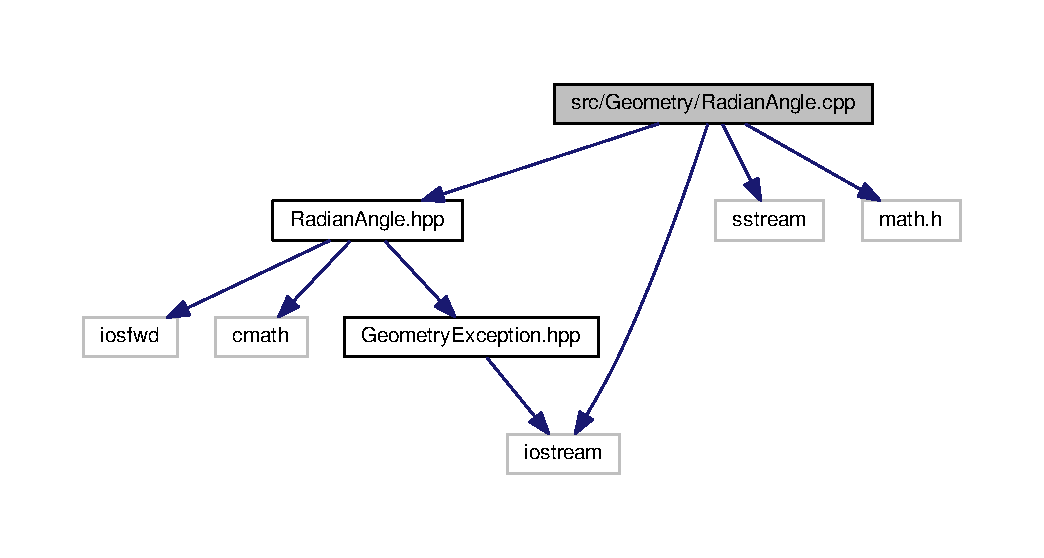
\includegraphics[width=350pt]{_radian_angle_8cpp__incl}
\end{center}
\end{figure}
\subsection*{Functions}
\begin{DoxyCompactItemize}
\item 
ostream \& \hyperlink{_radian_angle_8cpp_a19bc64edfd90b3e701d4e9fc173162e1}{operator$<$$<$} (ostream \&os, const \hyperlink{class_radian_angle}{Radian\+Angle} \&angle)
\item 
double \hyperlink{_radian_angle_8cpp_ab83046d4c4cf997bee757902750f229d}{cos} (const \hyperlink{class_radian_angle}{Radian\+Angle} \&angle)
\item 
double \hyperlink{_radian_angle_8cpp_a1c147c9e838e8f4806f9b7353f3165d4}{sin} (const \hyperlink{class_radian_angle}{Radian\+Angle} \&angle)
\end{DoxyCompactItemize}


\subsection{Function Documentation}
\hypertarget{_radian_angle_8cpp_ab83046d4c4cf997bee757902750f229d}{}\label{_radian_angle_8cpp_ab83046d4c4cf997bee757902750f229d} 
\index{Radian\+Angle.\+cpp@{Radian\+Angle.\+cpp}!cos@{cos}}
\index{cos@{cos}!Radian\+Angle.\+cpp@{Radian\+Angle.\+cpp}}
\subsubsection{\texorpdfstring{cos()}{cos()}}
{\footnotesize\ttfamily double cos (\begin{DoxyParamCaption}\item[{const \hyperlink{class_radian_angle}{Radian\+Angle} \&}]{angle }\end{DoxyParamCaption})}

Override function cos for \hyperlink{class_radian_angle}{Radian\+Angle} 
\begin{DoxyParams}{Parameters}
{\em angle} & \hyperlink{class_radian_angle}{Radian\+Angle} have to calculate \\
\hline
\end{DoxyParams}
\hypertarget{_radian_angle_8cpp_a19bc64edfd90b3e701d4e9fc173162e1}{}\label{_radian_angle_8cpp_a19bc64edfd90b3e701d4e9fc173162e1} 
\index{Radian\+Angle.\+cpp@{Radian\+Angle.\+cpp}!operator$<$$<$@{operator$<$$<$}}
\index{operator$<$$<$@{operator$<$$<$}!Radian\+Angle.\+cpp@{Radian\+Angle.\+cpp}}
\subsubsection{\texorpdfstring{operator$<$$<$()}{operator<<()}}
{\footnotesize\ttfamily ostream\& operator$<$$<$ (\begin{DoxyParamCaption}\item[{ostream \&}]{os,  }\item[{const \hyperlink{class_radian_angle}{Radian\+Angle} \&}]{angle }\end{DoxyParamCaption})}

Sends a string of angle to a stream 
\begin{DoxyParams}{Parameters}
{\em os} & ostream \\
\hline
{\em angle} & the angle to send \\
\hline
\end{DoxyParams}
\begin{DoxyReturn}{Returns}
ostream to send to output 
\end{DoxyReturn}
\hypertarget{_radian_angle_8cpp_a1c147c9e838e8f4806f9b7353f3165d4}{}\label{_radian_angle_8cpp_a1c147c9e838e8f4806f9b7353f3165d4} 
\index{Radian\+Angle.\+cpp@{Radian\+Angle.\+cpp}!sin@{sin}}
\index{sin@{sin}!Radian\+Angle.\+cpp@{Radian\+Angle.\+cpp}}
\subsubsection{\texorpdfstring{sin()}{sin()}}
{\footnotesize\ttfamily double sin (\begin{DoxyParamCaption}\item[{const \hyperlink{class_radian_angle}{Radian\+Angle} \&}]{angle }\end{DoxyParamCaption})}

Override function sin for \hyperlink{class_radian_angle}{Radian\+Angle} 
\begin{DoxyParams}{Parameters}
{\em angle} & \hyperlink{class_radian_angle}{Radian\+Angle} have to calculate \\
\hline
\end{DoxyParams}

\hypertarget{_radian_angle_8hpp}{}\section{src/\+Geometry/\+Radian\+Angle.hpp File Reference}
\label{_radian_angle_8hpp}\index{src/\+Geometry/\+Radian\+Angle.\+hpp@{src/\+Geometry/\+Radian\+Angle.\+hpp}}
{\ttfamily \#include $<$iosfwd$>$}\newline
{\ttfamily \#include $<$cmath$>$}\newline
{\ttfamily \#include \char`\"{}Geometry\+Exception.\+hpp\char`\"{}}\newline
Include dependency graph for Radian\+Angle.\+hpp\+:\nopagebreak
\begin{figure}[H]
\begin{center}
\leavevmode
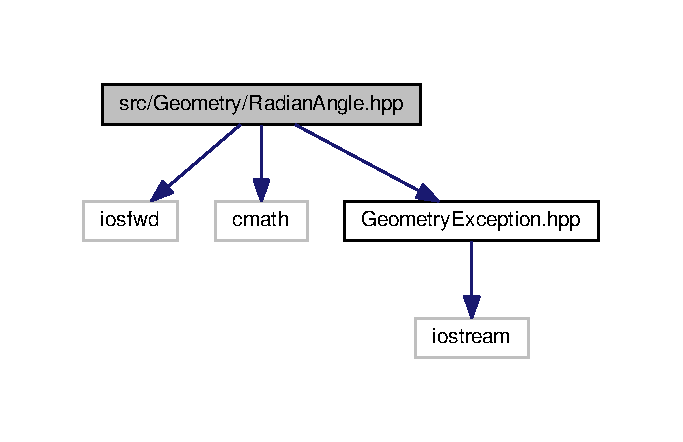
\includegraphics[width=328pt]{_radian_angle_8hpp__incl}
\end{center}
\end{figure}
This graph shows which files directly or indirectly include this file\+:\nopagebreak
\begin{figure}[H]
\begin{center}
\leavevmode
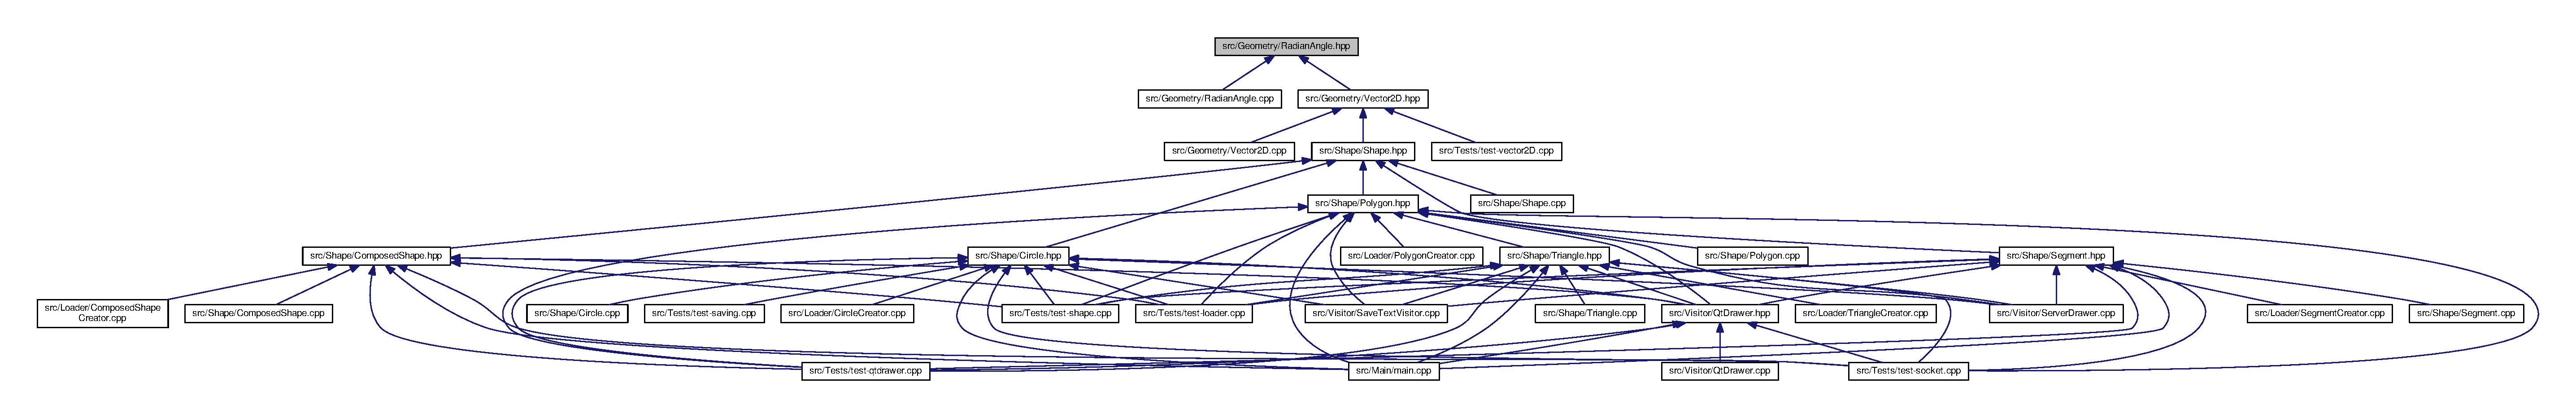
\includegraphics[width=350pt]{_radian_angle_8hpp__dep__incl}
\end{center}
\end{figure}
\subsection*{Classes}
\begin{DoxyCompactItemize}
\item 
class \hyperlink{class_radian_angle}{Radian\+Angle}
\end{DoxyCompactItemize}
\subsection*{Functions}
\begin{DoxyCompactItemize}
\item 
ostream \& \hyperlink{_radian_angle_8hpp_a19bc64edfd90b3e701d4e9fc173162e1}{operator$<$$<$} (ostream \&os, const \hyperlink{class_radian_angle}{Radian\+Angle} \&angle)
\item 
double \hyperlink{_radian_angle_8hpp_ab83046d4c4cf997bee757902750f229d}{cos} (const \hyperlink{class_radian_angle}{Radian\+Angle} \&angle)
\item 
double \hyperlink{_radian_angle_8hpp_a1c147c9e838e8f4806f9b7353f3165d4}{sin} (const \hyperlink{class_radian_angle}{Radian\+Angle} \&angle)
\end{DoxyCompactItemize}


\subsection{Function Documentation}
\hypertarget{_radian_angle_8hpp_ab83046d4c4cf997bee757902750f229d}{}\label{_radian_angle_8hpp_ab83046d4c4cf997bee757902750f229d} 
\index{Radian\+Angle.\+hpp@{Radian\+Angle.\+hpp}!cos@{cos}}
\index{cos@{cos}!Radian\+Angle.\+hpp@{Radian\+Angle.\+hpp}}
\subsubsection{\texorpdfstring{cos()}{cos()}}
{\footnotesize\ttfamily double cos (\begin{DoxyParamCaption}\item[{const \hyperlink{class_radian_angle}{Radian\+Angle} \&}]{angle }\end{DoxyParamCaption})}

Override function cos for \hyperlink{class_radian_angle}{Radian\+Angle} 
\begin{DoxyParams}{Parameters}
{\em angle} & \hyperlink{class_radian_angle}{Radian\+Angle} have to calculate \\
\hline
\end{DoxyParams}
\hypertarget{_radian_angle_8hpp_a19bc64edfd90b3e701d4e9fc173162e1}{}\label{_radian_angle_8hpp_a19bc64edfd90b3e701d4e9fc173162e1} 
\index{Radian\+Angle.\+hpp@{Radian\+Angle.\+hpp}!operator$<$$<$@{operator$<$$<$}}
\index{operator$<$$<$@{operator$<$$<$}!Radian\+Angle.\+hpp@{Radian\+Angle.\+hpp}}
\subsubsection{\texorpdfstring{operator$<$$<$()}{operator<<()}}
{\footnotesize\ttfamily ostream\& operator$<$$<$ (\begin{DoxyParamCaption}\item[{ostream \&}]{os,  }\item[{const \hyperlink{class_radian_angle}{Radian\+Angle} \&}]{angle }\end{DoxyParamCaption})}

Sends a string of angle to a stream 
\begin{DoxyParams}{Parameters}
{\em os} & ostream \\
\hline
{\em angle} & the angle to send \\
\hline
\end{DoxyParams}
\begin{DoxyReturn}{Returns}
ostream to send to output 
\end{DoxyReturn}
\hypertarget{_radian_angle_8hpp_a1c147c9e838e8f4806f9b7353f3165d4}{}\label{_radian_angle_8hpp_a1c147c9e838e8f4806f9b7353f3165d4} 
\index{Radian\+Angle.\+hpp@{Radian\+Angle.\+hpp}!sin@{sin}}
\index{sin@{sin}!Radian\+Angle.\+hpp@{Radian\+Angle.\+hpp}}
\subsubsection{\texorpdfstring{sin()}{sin()}}
{\footnotesize\ttfamily double sin (\begin{DoxyParamCaption}\item[{const \hyperlink{class_radian_angle}{Radian\+Angle} \&}]{angle }\end{DoxyParamCaption})}

Override function sin for \hyperlink{class_radian_angle}{Radian\+Angle} 
\begin{DoxyParams}{Parameters}
{\em angle} & \hyperlink{class_radian_angle}{Radian\+Angle} have to calculate \\
\hline
\end{DoxyParams}

\hypertarget{_vector2_d_8cpp}{}\section{src/\+Geometry/\+Vector2D.cpp File Reference}
\label{_vector2_d_8cpp}\index{src/\+Geometry/\+Vector2\+D.\+cpp@{src/\+Geometry/\+Vector2\+D.\+cpp}}
{\ttfamily \#include \char`\"{}Vector2\+D.\+hpp\char`\"{}}\newline
{\ttfamily \#include $<$sstream$>$}\newline
{\ttfamily \#include $<$iostream$>$}\newline
Include dependency graph for Vector2\+D.\+cpp\+:\nopagebreak
\begin{figure}[H]
\begin{center}
\leavevmode
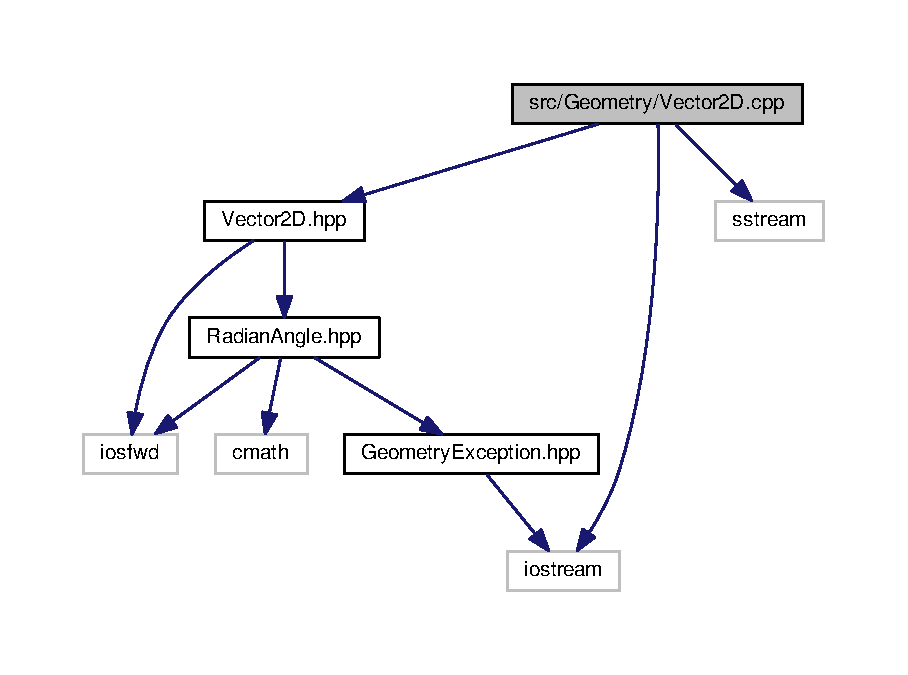
\includegraphics[width=350pt]{_vector2_d_8cpp__incl}
\end{center}
\end{figure}
\subsection*{Functions}
\begin{DoxyCompactItemize}
\item 
const \hyperlink{class_vector2_d}{Vector2D} \hyperlink{_vector2_d_8cpp_ad3f3c95069731f1cd8102ed44ea18029}{operator$\ast$} (const double \&a, const \hyperlink{class_vector2_d}{Vector2D} \&vector)
\item 
ostream \& \hyperlink{_vector2_d_8cpp_a947884ffef441f605f61b9bb1a2dab13}{operator$<$$<$} (ostream \&os, const \hyperlink{class_vector2_d}{Vector2D} \&vector)
\end{DoxyCompactItemize}


\subsection{Function Documentation}
\hypertarget{_vector2_d_8cpp_ad3f3c95069731f1cd8102ed44ea18029}{}\label{_vector2_d_8cpp_ad3f3c95069731f1cd8102ed44ea18029} 
\index{Vector2\+D.\+cpp@{Vector2\+D.\+cpp}!operator$\ast$@{operator$\ast$}}
\index{operator$\ast$@{operator$\ast$}!Vector2\+D.\+cpp@{Vector2\+D.\+cpp}}
\subsubsection{\texorpdfstring{operator$\ast$()}{operator*()}}
{\footnotesize\ttfamily const \hyperlink{class_vector2_d}{Vector2D} operator$\ast$ (\begin{DoxyParamCaption}\item[{const double \&}]{a,  }\item[{const \hyperlink{class_vector2_d}{Vector2D} \&}]{vector }\end{DoxyParamCaption})}

\hypertarget{_vector2_d_8cpp_a947884ffef441f605f61b9bb1a2dab13}{}\label{_vector2_d_8cpp_a947884ffef441f605f61b9bb1a2dab13} 
\index{Vector2\+D.\+cpp@{Vector2\+D.\+cpp}!operator$<$$<$@{operator$<$$<$}}
\index{operator$<$$<$@{operator$<$$<$}!Vector2\+D.\+cpp@{Vector2\+D.\+cpp}}
\subsubsection{\texorpdfstring{operator$<$$<$()}{operator<<()}}
{\footnotesize\ttfamily ostream\& operator$<$$<$ (\begin{DoxyParamCaption}\item[{ostream \&}]{os,  }\item[{const \hyperlink{class_vector2_d}{Vector2D} \&}]{vector }\end{DoxyParamCaption})}

Sends a string of vector to a stream 
\begin{DoxyParams}{Parameters}
{\em os} & ostream \\
\hline
{\em vector} & vector have to print \\
\hline
\end{DoxyParams}
\begin{DoxyReturn}{Returns}
ostream to send to the output 
\end{DoxyReturn}

\hypertarget{_vector2_d_8hpp}{}\section{src/\+Geometry/\+Vector2D.hpp File Reference}
\label{_vector2_d_8hpp}\index{src/\+Geometry/\+Vector2\+D.\+hpp@{src/\+Geometry/\+Vector2\+D.\+hpp}}
{\ttfamily \#include $<$iosfwd$>$}\newline
{\ttfamily \#include \char`\"{}Radian\+Angle.\+hpp\char`\"{}}\newline
Include dependency graph for Vector2\+D.\+hpp\+:\nopagebreak
\begin{figure}[H]
\begin{center}
\leavevmode
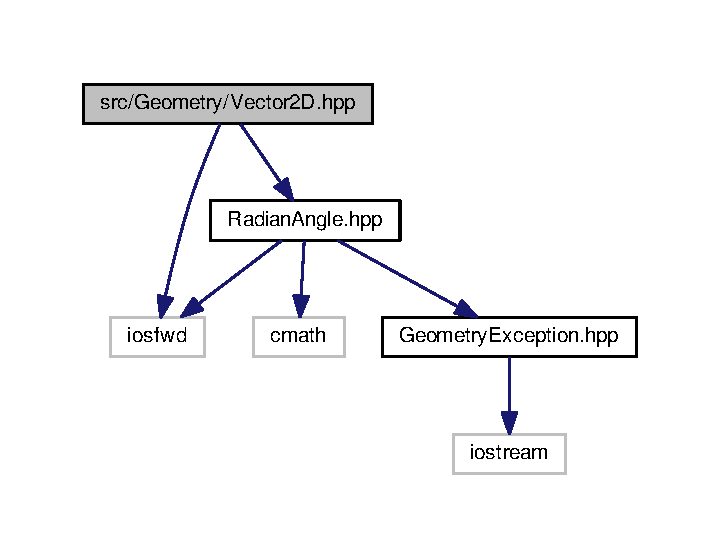
\includegraphics[width=346pt]{_vector2_d_8hpp__incl}
\end{center}
\end{figure}
This graph shows which files directly or indirectly include this file\+:\nopagebreak
\begin{figure}[H]
\begin{center}
\leavevmode
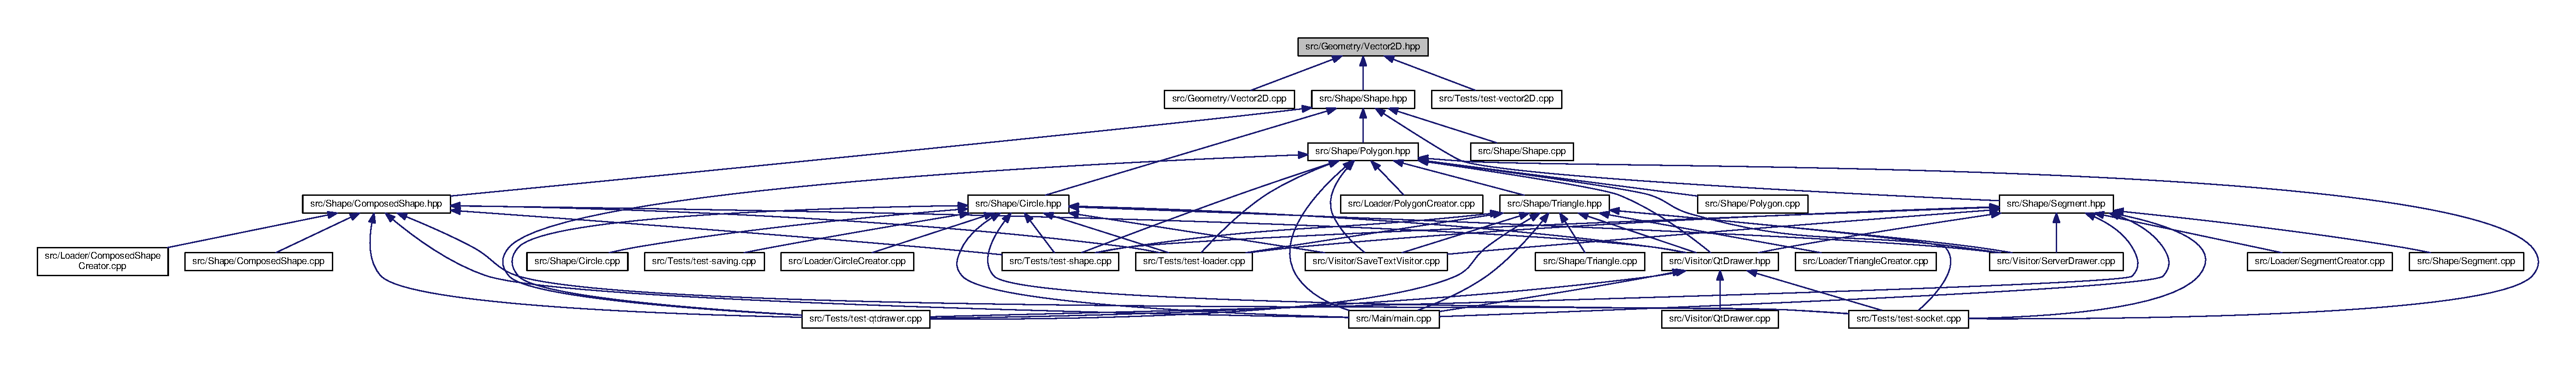
\includegraphics[width=350pt]{_vector2_d_8hpp__dep__incl}
\end{center}
\end{figure}
\subsection*{Classes}
\begin{DoxyCompactItemize}
\item 
class \hyperlink{class_vector2_d}{Vector2D}
\end{DoxyCompactItemize}
\subsection*{Functions}
\begin{DoxyCompactItemize}
\item 
const \hyperlink{class_vector2_d}{Vector2D} \hyperlink{_vector2_d_8hpp_ad3f3c95069731f1cd8102ed44ea18029}{operator$\ast$} (const double \&a, const \hyperlink{class_vector2_d}{Vector2D} \&vector)
\item 
ostream \& \hyperlink{_vector2_d_8hpp_a947884ffef441f605f61b9bb1a2dab13}{operator$<$$<$} (ostream \&os, const \hyperlink{class_vector2_d}{Vector2D} \&vector)
\end{DoxyCompactItemize}


\subsection{Function Documentation}
\hypertarget{_vector2_d_8hpp_ad3f3c95069731f1cd8102ed44ea18029}{}\label{_vector2_d_8hpp_ad3f3c95069731f1cd8102ed44ea18029} 
\index{Vector2\+D.\+hpp@{Vector2\+D.\+hpp}!operator$\ast$@{operator$\ast$}}
\index{operator$\ast$@{operator$\ast$}!Vector2\+D.\+hpp@{Vector2\+D.\+hpp}}
\subsubsection{\texorpdfstring{operator$\ast$()}{operator*()}}
{\footnotesize\ttfamily const \hyperlink{class_vector2_d}{Vector2D} operator$\ast$ (\begin{DoxyParamCaption}\item[{const double \&}]{a,  }\item[{const \hyperlink{class_vector2_d}{Vector2D} \&}]{vector }\end{DoxyParamCaption})}

\hypertarget{_vector2_d_8hpp_a947884ffef441f605f61b9bb1a2dab13}{}\label{_vector2_d_8hpp_a947884ffef441f605f61b9bb1a2dab13} 
\index{Vector2\+D.\+hpp@{Vector2\+D.\+hpp}!operator$<$$<$@{operator$<$$<$}}
\index{operator$<$$<$@{operator$<$$<$}!Vector2\+D.\+hpp@{Vector2\+D.\+hpp}}
\subsubsection{\texorpdfstring{operator$<$$<$()}{operator<<()}}
{\footnotesize\ttfamily ostream\& operator$<$$<$ (\begin{DoxyParamCaption}\item[{ostream \&}]{os,  }\item[{const \hyperlink{class_vector2_d}{Vector2D} \&}]{vector }\end{DoxyParamCaption})}

Sends a string of vector to a stream 
\begin{DoxyParams}{Parameters}
{\em os} & ostream \\
\hline
{\em vector} & vector have to print \\
\hline
\end{DoxyParams}
\begin{DoxyReturn}{Returns}
ostream to send to the output 
\end{DoxyReturn}

\hypertarget{_circle_creator_8cpp}{}\section{src/\+Loader/\+Circle\+Creator.cpp File Reference}
\label{_circle_creator_8cpp}\index{src/\+Loader/\+Circle\+Creator.\+cpp@{src/\+Loader/\+Circle\+Creator.\+cpp}}
{\ttfamily \#include \char`\"{}Circle\+Creator.\+hpp\char`\"{}}\newline
{\ttfamily \#include \char`\"{}Shape\+Loader\+Exception.\+hpp\char`\"{}}\newline
{\ttfamily \#include \char`\"{}../\+Shape/\+Circle.\+hpp\char`\"{}}\newline
{\ttfamily \#include $<$iostream$>$}\newline
{\ttfamily \#include $<$cstdlib$>$}\newline
Include dependency graph for Circle\+Creator.\+cpp\+:\nopagebreak
\begin{figure}[H]
\begin{center}
\leavevmode
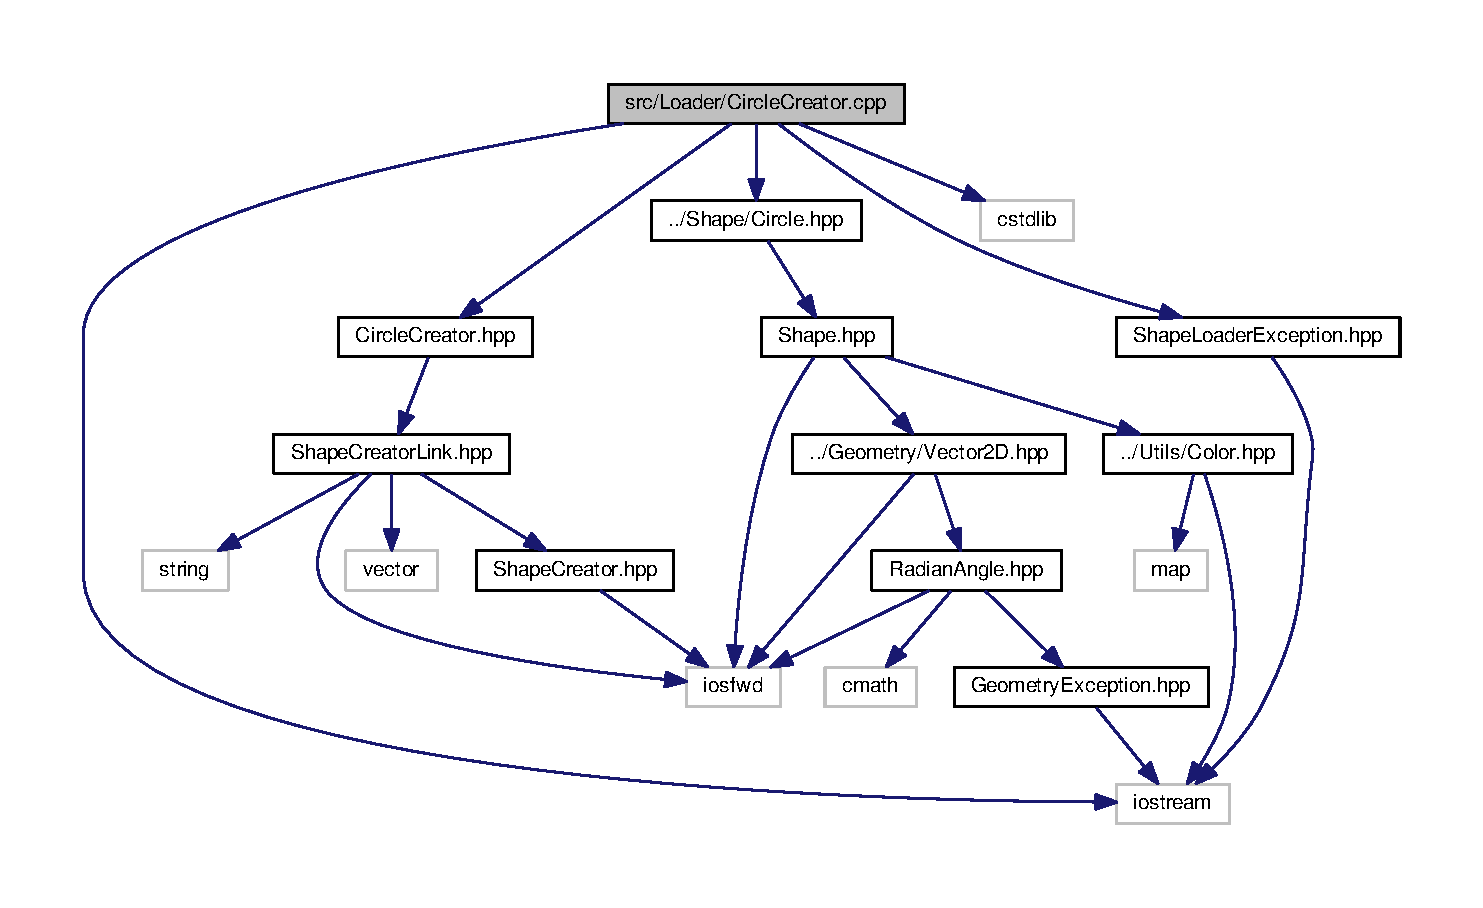
\includegraphics[width=350pt]{_circle_creator_8cpp__incl}
\end{center}
\end{figure}

\hypertarget{_circle_creator_8hpp}{}\section{src/\+Loader/\+Circle\+Creator.hpp File Reference}
\label{_circle_creator_8hpp}\index{src/\+Loader/\+Circle\+Creator.\+hpp@{src/\+Loader/\+Circle\+Creator.\+hpp}}
{\ttfamily \#include \char`\"{}Shape\+Creator\+Link.\+hpp\char`\"{}}\newline
Include dependency graph for Circle\+Creator.\+hpp\+:\nopagebreak
\begin{figure}[H]
\begin{center}
\leavevmode
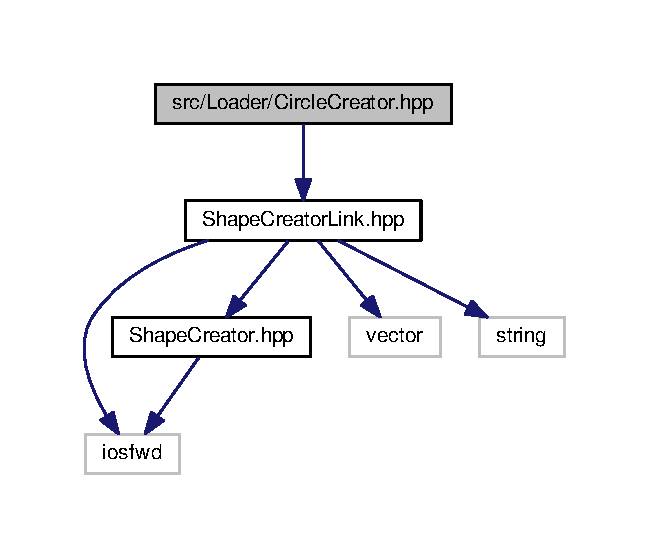
\includegraphics[width=311pt]{_circle_creator_8hpp__incl}
\end{center}
\end{figure}
This graph shows which files directly or indirectly include this file\+:
\nopagebreak
\begin{figure}[H]
\begin{center}
\leavevmode
\includegraphics[width=350pt]{_circle_creator_8hpp__dep__incl}
\end{center}
\end{figure}
\subsection*{Classes}
\begin{DoxyCompactItemize}
\item 
class \hyperlink{class_circle_creator}{Circle\+Creator}
\end{DoxyCompactItemize}

\hypertarget{_composed_shape_creator_8cpp}{}\section{src/\+Loader/\+Composed\+Shape\+Creator.cpp File Reference}
\label{_composed_shape_creator_8cpp}\index{src/\+Loader/\+Composed\+Shape\+Creator.\+cpp@{src/\+Loader/\+Composed\+Shape\+Creator.\+cpp}}
{\ttfamily \#include \char`\"{}Composed\+Shape\+Creator.\+hpp\char`\"{}}\newline
{\ttfamily \#include \char`\"{}Shape\+Loader\+Exception.\+hpp\char`\"{}}\newline
{\ttfamily \#include \char`\"{}../\+Shape/\+Composed\+Shape.\+hpp\char`\"{}}\newline
{\ttfamily \#include $<$iostream$>$}\newline
{\ttfamily \#include $<$cstdlib$>$}\newline
Include dependency graph for Composed\+Shape\+Creator.\+cpp\+:\nopagebreak
\begin{figure}[H]
\begin{center}
\leavevmode
\includegraphics[width=350pt]{_composed_shape_creator_8cpp__incl}
\end{center}
\end{figure}

\hypertarget{_composed_shape_creator_8hpp}{}\section{src/\+Loader/\+Composed\+Shape\+Creator.hpp File Reference}
\label{_composed_shape_creator_8hpp}\index{src/\+Loader/\+Composed\+Shape\+Creator.\+hpp@{src/\+Loader/\+Composed\+Shape\+Creator.\+hpp}}
{\ttfamily \#include \char`\"{}Shape\+Creator\+Link.\+hpp\char`\"{}}\newline
Include dependency graph for Composed\+Shape\+Creator.\+hpp\+:\nopagebreak
\begin{figure}[H]
\begin{center}
\leavevmode
\includegraphics[width=311pt]{_composed_shape_creator_8hpp__incl}
\end{center}
\end{figure}
This graph shows which files directly or indirectly include this file\+:
\nopagebreak
\begin{figure}[H]
\begin{center}
\leavevmode
\includegraphics[width=350pt]{_composed_shape_creator_8hpp__dep__incl}
\end{center}
\end{figure}
\subsection*{Classes}
\begin{DoxyCompactItemize}
\item 
class \hyperlink{class_composed_shape_creator}{Composed\+Shape\+Creator}
\end{DoxyCompactItemize}

\hypertarget{_polygon_creator_8cpp}{}\section{src/\+Loader/\+Polygon\+Creator.cpp File Reference}
\label{_polygon_creator_8cpp}\index{src/\+Loader/\+Polygon\+Creator.\+cpp@{src/\+Loader/\+Polygon\+Creator.\+cpp}}
{\ttfamily \#include \char`\"{}Polygon\+Creator.\+hpp\char`\"{}}\newline
{\ttfamily \#include \char`\"{}Shape\+Loader\+Exception.\+hpp\char`\"{}}\newline
{\ttfamily \#include \char`\"{}../\+Shape/\+Polygon.\+hpp\char`\"{}}\newline
{\ttfamily \#include $<$iostream$>$}\newline
{\ttfamily \#include $<$cstdlib$>$}\newline
Include dependency graph for Polygon\+Creator.\+cpp\+:\nopagebreak
\begin{figure}[H]
\begin{center}
\leavevmode
\includegraphics[width=350pt]{_polygon_creator_8cpp__incl}
\end{center}
\end{figure}

\hypertarget{_polygon_creator_8hpp}{}\section{src/\+Loader/\+Polygon\+Creator.hpp File Reference}
\label{_polygon_creator_8hpp}\index{src/\+Loader/\+Polygon\+Creator.\+hpp@{src/\+Loader/\+Polygon\+Creator.\+hpp}}
{\ttfamily \#include \char`\"{}Shape\+Creator\+Link.\+hpp\char`\"{}}\newline
Include dependency graph for Polygon\+Creator.\+hpp\+:\nopagebreak
\begin{figure}[H]
\begin{center}
\leavevmode
\includegraphics[width=311pt]{_polygon_creator_8hpp__incl}
\end{center}
\end{figure}
This graph shows which files directly or indirectly include this file\+:
\nopagebreak
\begin{figure}[H]
\begin{center}
\leavevmode
\includegraphics[width=350pt]{_polygon_creator_8hpp__dep__incl}
\end{center}
\end{figure}
\subsection*{Classes}
\begin{DoxyCompactItemize}
\item 
class \hyperlink{class_polygon_creator}{Polygon\+Creator}
\end{DoxyCompactItemize}

\hypertarget{_segment_creator_8cpp}{}\section{src/\+Loader/\+Segment\+Creator.cpp File Reference}
\label{_segment_creator_8cpp}\index{src/\+Loader/\+Segment\+Creator.\+cpp@{src/\+Loader/\+Segment\+Creator.\+cpp}}
{\ttfamily \#include \char`\"{}Segment\+Creator.\+hpp\char`\"{}}\newline
{\ttfamily \#include \char`\"{}Shape\+Loader\+Exception.\+hpp\char`\"{}}\newline
{\ttfamily \#include \char`\"{}../\+Shape/\+Segment.\+hpp\char`\"{}}\newline
{\ttfamily \#include $<$iostream$>$}\newline
{\ttfamily \#include $<$cstdlib$>$}\newline
Include dependency graph for Segment\+Creator.\+cpp\+:\nopagebreak
\begin{figure}[H]
\begin{center}
\leavevmode
\includegraphics[width=350pt]{_segment_creator_8cpp__incl}
\end{center}
\end{figure}

\hypertarget{_segment_creator_8hpp}{}\section{src/\+Loader/\+Segment\+Creator.hpp File Reference}
\label{_segment_creator_8hpp}\index{src/\+Loader/\+Segment\+Creator.\+hpp@{src/\+Loader/\+Segment\+Creator.\+hpp}}
{\ttfamily \#include \char`\"{}Shape\+Creator\+Link.\+hpp\char`\"{}}\newline
Include dependency graph for Segment\+Creator.\+hpp\+:\nopagebreak
\begin{figure}[H]
\begin{center}
\leavevmode
\includegraphics[width=311pt]{_segment_creator_8hpp__incl}
\end{center}
\end{figure}
This graph shows which files directly or indirectly include this file\+:
\nopagebreak
\begin{figure}[H]
\begin{center}
\leavevmode
\includegraphics[width=350pt]{_segment_creator_8hpp__dep__incl}
\end{center}
\end{figure}
\subsection*{Classes}
\begin{DoxyCompactItemize}
\item 
class \hyperlink{class_segment_creator}{Segment\+Creator}
\end{DoxyCompactItemize}

\hypertarget{_shape_creator_8hpp}{}\section{src/\+Loader/\+Shape\+Creator.hpp File Reference}
\label{_shape_creator_8hpp}\index{src/\+Loader/\+Shape\+Creator.\+hpp@{src/\+Loader/\+Shape\+Creator.\+hpp}}
{\ttfamily \#include $<$iosfwd$>$}\newline
Include dependency graph for Shape\+Creator.\+hpp\+:\nopagebreak
\begin{figure}[H]
\begin{center}
\leavevmode
\includegraphics[width=224pt]{_shape_creator_8hpp__incl}
\end{center}
\end{figure}
This graph shows which files directly or indirectly include this file\+:
\nopagebreak
\begin{figure}[H]
\begin{center}
\leavevmode
\includegraphics[width=350pt]{_shape_creator_8hpp__dep__incl}
\end{center}
\end{figure}
\subsection*{Classes}
\begin{DoxyCompactItemize}
\item 
class \hyperlink{class_shape_creator}{Shape\+Creator}
\end{DoxyCompactItemize}

\hypertarget{_shape_creator_link_8cpp}{}\section{src/\+Loader/\+Shape\+Creator\+Link.cpp File Reference}
\label{_shape_creator_link_8cpp}\index{src/\+Loader/\+Shape\+Creator\+Link.\+cpp@{src/\+Loader/\+Shape\+Creator\+Link.\+cpp}}
{\ttfamily \#include \char`\"{}Shape\+Creator\+Link.\+hpp\char`\"{}}\newline
{\ttfamily \#include \char`\"{}Shape\+Loader\+Exception.\+hpp\char`\"{}}\newline
{\ttfamily \#include $<$iostream$>$}\newline
Include dependency graph for Shape\+Creator\+Link.\+cpp\+:\nopagebreak
\begin{figure}[H]
\begin{center}
\leavevmode
\includegraphics[width=350pt]{_shape_creator_link_8cpp__incl}
\end{center}
\end{figure}

\hypertarget{_shape_creator_link_8hpp}{}\section{src/\+Loader/\+Shape\+Creator\+Link.hpp File Reference}
\label{_shape_creator_link_8hpp}\index{src/\+Loader/\+Shape\+Creator\+Link.\+hpp@{src/\+Loader/\+Shape\+Creator\+Link.\+hpp}}
{\ttfamily \#include $<$iosfwd$>$}\newline
{\ttfamily \#include \char`\"{}Shape\+Creator.\+hpp\char`\"{}}\newline
{\ttfamily \#include $<$vector$>$}\newline
{\ttfamily \#include $<$string$>$}\newline
Include dependency graph for Shape\+Creator\+Link.\+hpp\+:\nopagebreak
\begin{figure}[H]
\begin{center}
\leavevmode
\includegraphics[width=311pt]{_shape_creator_link_8hpp__incl}
\end{center}
\end{figure}
This graph shows which files directly or indirectly include this file\+:
\nopagebreak
\begin{figure}[H]
\begin{center}
\leavevmode
\includegraphics[width=350pt]{_shape_creator_link_8hpp__dep__incl}
\end{center}
\end{figure}
\subsection*{Classes}
\begin{DoxyCompactItemize}
\item 
class \hyperlink{class_shape_creator_link}{Shape\+Creator\+Link}
\end{DoxyCompactItemize}
\subsection*{Namespaces}
\begin{DoxyCompactItemize}
\item 
 \hyperlink{namespacefunc}{func}
\end{DoxyCompactItemize}
\subsection*{Functions}
\begin{DoxyCompactItemize}
\item 
vector$<$ string $>$ \hyperlink{namespacefunc_a9f72ec6e5c1c3620723c349a075d2298}{func\+::split} (const string \&s, char sep)
\end{DoxyCompactItemize}

\hypertarget{_shape_loader_8hpp}{}\section{src/\+Loader/\+Shape\+Loader.hpp File Reference}
\label{_shape_loader_8hpp}\index{src/\+Loader/\+Shape\+Loader.\+hpp@{src/\+Loader/\+Shape\+Loader.\+hpp}}
{\ttfamily \#include $<$iosfwd$>$}\newline
Include dependency graph for Shape\+Loader.\+hpp\+:\nopagebreak
\begin{figure}[H]
\begin{center}
\leavevmode
\includegraphics[width=221pt]{_shape_loader_8hpp__incl}
\end{center}
\end{figure}
This graph shows which files directly or indirectly include this file\+:
\nopagebreak
\begin{figure}[H]
\begin{center}
\leavevmode
\includegraphics[width=350pt]{_shape_loader_8hpp__dep__incl}
\end{center}
\end{figure}
\subsection*{Classes}
\begin{DoxyCompactItemize}
\item 
class \hyperlink{class_shape_loader}{Shape\+Loader}
\end{DoxyCompactItemize}

\hypertarget{_shape_loader_exception_8cpp}{}\section{src/\+Loader/\+Shape\+Loader\+Exception.cpp File Reference}
\label{_shape_loader_exception_8cpp}\index{src/\+Loader/\+Shape\+Loader\+Exception.\+cpp@{src/\+Loader/\+Shape\+Loader\+Exception.\+cpp}}
{\ttfamily \#include \char`\"{}Shape\+Loader\+Exception.\+hpp\char`\"{}}\newline
Include dependency graph for Shape\+Loader\+Exception.\+cpp\+:\nopagebreak
\begin{figure}[H]
\begin{center}
\leavevmode
\includegraphics[width=265pt]{_shape_loader_exception_8cpp__incl}
\end{center}
\end{figure}
\subsection*{Functions}
\begin{DoxyCompactItemize}
\item 
ostream \& \hyperlink{_shape_loader_exception_8cpp_a9db19dba46ba71d9fc2a1bd72f141364}{operator$<$$<$} (ostream \&os, const \hyperlink{class_shape_loader_exception}{Shape\+Loader\+Exception} \&\hyperlink{class_shape_loader_exception}{Shape\+Loader\+Exception})
\end{DoxyCompactItemize}


\subsection{Function Documentation}
\hypertarget{_shape_loader_exception_8cpp_a9db19dba46ba71d9fc2a1bd72f141364}{}\label{_shape_loader_exception_8cpp_a9db19dba46ba71d9fc2a1bd72f141364} 
\index{Shape\+Loader\+Exception.\+cpp@{Shape\+Loader\+Exception.\+cpp}!operator$<$$<$@{operator$<$$<$}}
\index{operator$<$$<$@{operator$<$$<$}!Shape\+Loader\+Exception.\+cpp@{Shape\+Loader\+Exception.\+cpp}}
\subsubsection{\texorpdfstring{operator$<$$<$()}{operator<<()}}
{\footnotesize\ttfamily ostream\& operator$<$$<$ (\begin{DoxyParamCaption}\item[{ostream \&}]{os,  }\item[{const \hyperlink{class_shape_loader_exception}{Shape\+Loader\+Exception} \&}]{Shape\+Loader\+Exception }\end{DoxyParamCaption})}

Sends a string of excpetion to a stream 
\begin{DoxyParams}{Parameters}
{\em os} & ostream \\
\hline
{\em \hyperlink{class_shape_loader_exception}{Shape\+Loader\+Exception}} & \hyperlink{class_shape_loader_exception}{Shape\+Loader\+Exception} have to print \\
\hline
\end{DoxyParams}
\begin{DoxyReturn}{Returns}
ostream to send to the output 
\end{DoxyReturn}

\hypertarget{_shape_loader_exception_8hpp}{}\section{src/\+Loader/\+Shape\+Loader\+Exception.hpp File Reference}
\label{_shape_loader_exception_8hpp}\index{src/\+Loader/\+Shape\+Loader\+Exception.\+hpp@{src/\+Loader/\+Shape\+Loader\+Exception.\+hpp}}
{\ttfamily \#include $<$iostream$>$}\newline
Include dependency graph for Shape\+Loader\+Exception.\+hpp\+:\nopagebreak
\begin{figure}[H]
\begin{center}
\leavevmode
\includegraphics[width=265pt]{_shape_loader_exception_8hpp__incl}
\end{center}
\end{figure}
This graph shows which files directly or indirectly include this file\+:
\nopagebreak
\begin{figure}[H]
\begin{center}
\leavevmode
\includegraphics[width=350pt]{_shape_loader_exception_8hpp__dep__incl}
\end{center}
\end{figure}
\subsection*{Classes}
\begin{DoxyCompactItemize}
\item 
class \hyperlink{class_shape_loader_exception}{Shape\+Loader\+Exception}
\end{DoxyCompactItemize}
\subsection*{Functions}
\begin{DoxyCompactItemize}
\item 
ostream \& \hyperlink{_shape_loader_exception_8hpp_aaeb686a05fcc919d9b383b9f61182f44}{operator$<$$<$} (ostream \&os, const \hyperlink{class_shape_loader_exception}{Shape\+Loader\+Exception} \&shape\+Loader\+Exception)
\end{DoxyCompactItemize}


\subsection{Function Documentation}
\hypertarget{_shape_loader_exception_8hpp_aaeb686a05fcc919d9b383b9f61182f44}{}\label{_shape_loader_exception_8hpp_aaeb686a05fcc919d9b383b9f61182f44} 
\index{Shape\+Loader\+Exception.\+hpp@{Shape\+Loader\+Exception.\+hpp}!operator$<$$<$@{operator$<$$<$}}
\index{operator$<$$<$@{operator$<$$<$}!Shape\+Loader\+Exception.\+hpp@{Shape\+Loader\+Exception.\+hpp}}
\subsubsection{\texorpdfstring{operator$<$$<$()}{operator<<()}}
{\footnotesize\ttfamily ostream\& operator$<$$<$ (\begin{DoxyParamCaption}\item[{ostream \&}]{os,  }\item[{const \hyperlink{class_shape_loader_exception}{Shape\+Loader\+Exception} \&}]{Shape\+Loader\+Exception }\end{DoxyParamCaption})}

Sends a string of excpetion to a stream 
\begin{DoxyParams}{Parameters}
{\em os} & ostream \\
\hline
{\em \hyperlink{class_shape_loader_exception}{Shape\+Loader\+Exception}} & \hyperlink{class_shape_loader_exception}{Shape\+Loader\+Exception} have to print \\
\hline
\end{DoxyParams}
\begin{DoxyReturn}{Returns}
ostream to send to the output 
\end{DoxyReturn}

\hypertarget{_shape_loader_link_8cpp}{}\section{src/\+Loader/\+Shape\+Loader\+Link.cpp File Reference}
\label{_shape_loader_link_8cpp}\index{src/\+Loader/\+Shape\+Loader\+Link.\+cpp@{src/\+Loader/\+Shape\+Loader\+Link.\+cpp}}
{\ttfamily \#include \char`\"{}Shape\+Loader\+Link.\+hpp\char`\"{}}\newline
{\ttfamily \#include \char`\"{}Shape\+Loader\+Exception.\+hpp\char`\"{}}\newline
Include dependency graph for Shape\+Loader\+Link.\+cpp\+:\nopagebreak
\begin{figure}[H]
\begin{center}
\leavevmode
\includegraphics[width=344pt]{_shape_loader_link_8cpp__incl}
\end{center}
\end{figure}

\hypertarget{_shape_loader_link_8hpp}{}\section{src/\+Loader/\+Shape\+Loader\+Link.hpp File Reference}
\label{_shape_loader_link_8hpp}\index{src/\+Loader/\+Shape\+Loader\+Link.\+hpp@{src/\+Loader/\+Shape\+Loader\+Link.\+hpp}}
{\ttfamily \#include $<$iosfwd$>$}\newline
{\ttfamily \#include \char`\"{}Shape\+Loader.\+hpp\char`\"{}}\newline
Include dependency graph for Shape\+Loader\+Link.\+hpp\+:\nopagebreak
\begin{figure}[H]
\begin{center}
\leavevmode
\includegraphics[width=243pt]{_shape_loader_link_8hpp__incl}
\end{center}
\end{figure}
This graph shows which files directly or indirectly include this file\+:
\nopagebreak
\begin{figure}[H]
\begin{center}
\leavevmode
\includegraphics[width=350pt]{_shape_loader_link_8hpp__dep__incl}
\end{center}
\end{figure}
\subsection*{Classes}
\begin{DoxyCompactItemize}
\item 
class \hyperlink{class_shape_loader_link}{Shape\+Loader\+Link}
\end{DoxyCompactItemize}

\hypertarget{_shape_loader_text_8cpp}{}\section{src/\+Loader/\+Shape\+Loader\+Text.cpp File Reference}
\label{_shape_loader_text_8cpp}\index{src/\+Loader/\+Shape\+Loader\+Text.\+cpp@{src/\+Loader/\+Shape\+Loader\+Text.\+cpp}}
{\ttfamily \#include \char`\"{}Shape\+Loader\+Text.\+hpp\char`\"{}}\newline
{\ttfamily \#include \char`\"{}Shape\+Loader\+Exception.\+hpp\char`\"{}}\newline
{\ttfamily \#include \char`\"{}Shape\+Creator.\+hpp\char`\"{}}\newline
{\ttfamily \#include $<$iostream$>$}\newline
{\ttfamily \#include $<$string$>$}\newline
{\ttfamily \#include $<$cstddef$>$}\newline
{\ttfamily \#include $<$fstream$>$}\newline
{\ttfamily \#include $<$sstream$>$}\newline
Include dependency graph for Shape\+Loader\+Text.\+cpp\+:\nopagebreak
\begin{figure}[H]
\begin{center}
\leavevmode
\includegraphics[width=350pt]{_shape_loader_text_8cpp__incl}
\end{center}
\end{figure}

\hypertarget{_shape_loader_text_8hpp}{}\section{src/\+Loader/\+Shape\+Loader\+Text.hpp File Reference}
\label{_shape_loader_text_8hpp}\index{src/\+Loader/\+Shape\+Loader\+Text.\+hpp@{src/\+Loader/\+Shape\+Loader\+Text.\+hpp}}
{\ttfamily \#include \char`\"{}Shape\+Loader\+Link.\+hpp\char`\"{}}\newline
Include dependency graph for Shape\+Loader\+Text.\+hpp\+:\nopagebreak
\begin{figure}[H]
\begin{center}
\leavevmode
\includegraphics[width=244pt]{_shape_loader_text_8hpp__incl}
\end{center}
\end{figure}
This graph shows which files directly or indirectly include this file\+:
\nopagebreak
\begin{figure}[H]
\begin{center}
\leavevmode
\includegraphics[width=350pt]{_shape_loader_text_8hpp__dep__incl}
\end{center}
\end{figure}
\subsection*{Classes}
\begin{DoxyCompactItemize}
\item 
class \hyperlink{class_shape_loader_text}{Shape\+Loader\+Text}
\end{DoxyCompactItemize}

\hypertarget{_triangle_creator_8cpp}{}\section{src/\+Loader/\+Triangle\+Creator.cpp File Reference}
\label{_triangle_creator_8cpp}\index{src/\+Loader/\+Triangle\+Creator.\+cpp@{src/\+Loader/\+Triangle\+Creator.\+cpp}}
{\ttfamily \#include \char`\"{}Triangle\+Creator.\+hpp\char`\"{}}\newline
{\ttfamily \#include \char`\"{}Shape\+Loader\+Exception.\+hpp\char`\"{}}\newline
{\ttfamily \#include \char`\"{}../\+Shape/\+Triangle.\+hpp\char`\"{}}\newline
{\ttfamily \#include $<$iostream$>$}\newline
{\ttfamily \#include $<$cstdlib$>$}\newline
Include dependency graph for Triangle\+Creator.\+cpp\+:\nopagebreak
\begin{figure}[H]
\begin{center}
\leavevmode
\includegraphics[width=350pt]{_triangle_creator_8cpp__incl}
\end{center}
\end{figure}

\hypertarget{_triangle_creator_8hpp}{}\section{src/\+Loader/\+Triangle\+Creator.hpp File Reference}
\label{_triangle_creator_8hpp}\index{src/\+Loader/\+Triangle\+Creator.\+hpp@{src/\+Loader/\+Triangle\+Creator.\+hpp}}
{\ttfamily \#include \char`\"{}Shape\+Creator\+Link.\+hpp\char`\"{}}\newline
Include dependency graph for Triangle\+Creator.\+hpp\+:\nopagebreak
\begin{figure}[H]
\begin{center}
\leavevmode
\includegraphics[width=311pt]{_triangle_creator_8hpp__incl}
\end{center}
\end{figure}
This graph shows which files directly or indirectly include this file\+:
\nopagebreak
\begin{figure}[H]
\begin{center}
\leavevmode
\includegraphics[width=350pt]{_triangle_creator_8hpp__dep__incl}
\end{center}
\end{figure}
\subsection*{Classes}
\begin{DoxyCompactItemize}
\item 
class \hyperlink{class_triangle_creator}{Triangle\+Creator}
\end{DoxyCompactItemize}

\hypertarget{main_8cpp}{}\section{src/\+Main/main.cpp File Reference}
\label{main_8cpp}\index{src/\+Main/main.\+cpp@{src/\+Main/main.\+cpp}}
{\ttfamily \#include \char`\"{}../\+Network/\+Socket.\+hpp\char`\"{}}\newline
{\ttfamily \#include \char`\"{}../\+Visitor/\+Server\+Drawer.\+hpp\char`\"{}}\newline
{\ttfamily \#include \char`\"{}../\+Shape/\+Circle.\+hpp\char`\"{}}\newline
{\ttfamily \#include \char`\"{}../\+Shape/\+Polygon.\+hpp\char`\"{}}\newline
{\ttfamily \#include \char`\"{}../\+Shape/\+Triangle.\+hpp\char`\"{}}\newline
{\ttfamily \#include \char`\"{}../\+Shape/\+Segment.\+hpp\char`\"{}}\newline
{\ttfamily \#include \char`\"{}../\+Shape/\+Composed\+Shape.\+hpp\char`\"{}}\newline
{\ttfamily \#include \char`\"{}../\+Visitor/\+Qt\+Drawer.\+hpp\char`\"{}}\newline
{\ttfamily \#include \char`\"{}../\+Visitor/\+Save\+Text\+Visitor.\+hpp\char`\"{}}\newline
{\ttfamily \#include \char`\"{}../\+Loader/\+Segment\+Creator.\+hpp\char`\"{}}\newline
{\ttfamily \#include \char`\"{}../\+Loader/\+Triangle\+Creator.\+hpp\char`\"{}}\newline
{\ttfamily \#include \char`\"{}../\+Loader/\+Polygon\+Creator.\+hpp\char`\"{}}\newline
{\ttfamily \#include \char`\"{}../\+Loader/\+Circle\+Creator.\+hpp\char`\"{}}\newline
{\ttfamily \#include \char`\"{}../\+Loader/\+Composed\+Shape\+Creator.\+hpp\char`\"{}}\newline
{\ttfamily \#include \char`\"{}../\+Loader/\+Shape\+Loader\+Exception.\+hpp\char`\"{}}\newline
{\ttfamily \#include \char`\"{}../\+Loader/\+Shape\+Loader\+Text.\+hpp\char`\"{}}\newline
Include dependency graph for main.\+cpp\+:
\nopagebreak
\begin{figure}[H]
\begin{center}
\leavevmode
\includegraphics[width=350pt]{main_8cpp__incl}
\end{center}
\end{figure}
\subsection*{Functions}
\begin{DoxyCompactItemize}
\item 
int \hyperlink{main_8cpp_a0ddf1224851353fc92bfbff6f499fa97}{main} (int argc, char $\ast$argv\mbox{[}$\,$\mbox{]})
\end{DoxyCompactItemize}


\subsection{Function Documentation}
\hypertarget{main_8cpp_a0ddf1224851353fc92bfbff6f499fa97}{}\label{main_8cpp_a0ddf1224851353fc92bfbff6f499fa97} 
\index{main.\+cpp@{main.\+cpp}!main@{main}}
\index{main@{main}!main.\+cpp@{main.\+cpp}}
\subsubsection{\texorpdfstring{main()}{main()}}
{\footnotesize\ttfamily int main (\begin{DoxyParamCaption}\item[{int}]{argc,  }\item[{char $\ast$}]{argv\mbox{[}$\,$\mbox{]} }\end{DoxyParamCaption})}


\hypertarget{_network_exception_8cpp}{}\section{src/\+Network/\+Network\+Exception.cpp File Reference}
\label{_network_exception_8cpp}\index{src/\+Network/\+Network\+Exception.\+cpp@{src/\+Network/\+Network\+Exception.\+cpp}}
{\ttfamily \#include \char`\"{}Network\+Exception.\+hpp\char`\"{}}\newline
Include dependency graph for Network\+Exception.\+cpp\+:\nopagebreak
\begin{figure}[H]
\begin{center}
\leavevmode
\includegraphics[width=252pt]{_network_exception_8cpp__incl}
\end{center}
\end{figure}
\subsection*{Functions}
\begin{DoxyCompactItemize}
\item 
ostream \& \hyperlink{_network_exception_8cpp_a2c376f88177b93b2c3734294358fbef0}{operator$<$$<$} (ostream \&os, const \hyperlink{class_network_exception}{Network\+Exception} \&network\+Exception)
\end{DoxyCompactItemize}


\subsection{Function Documentation}
\hypertarget{_network_exception_8cpp_a2c376f88177b93b2c3734294358fbef0}{}\label{_network_exception_8cpp_a2c376f88177b93b2c3734294358fbef0} 
\index{Network\+Exception.\+cpp@{Network\+Exception.\+cpp}!operator$<$$<$@{operator$<$$<$}}
\index{operator$<$$<$@{operator$<$$<$}!Network\+Exception.\+cpp@{Network\+Exception.\+cpp}}
\subsubsection{\texorpdfstring{operator$<$$<$()}{operator<<()}}
{\footnotesize\ttfamily ostream\& operator$<$$<$ (\begin{DoxyParamCaption}\item[{ostream \&}]{os,  }\item[{const \hyperlink{class_network_exception}{Network\+Exception} \&}]{network\+Exception }\end{DoxyParamCaption})}

Sends a string of excpetion to a stream 
\begin{DoxyParams}{Parameters}
{\em os} & ostream \\
\hline
{\em \hyperlink{class_network_exception}{Network\+Exception}} & \hyperlink{class_network_exception}{Network\+Exception} have to print \\
\hline
\end{DoxyParams}
\begin{DoxyReturn}{Returns}
ostream to send to the output 
\end{DoxyReturn}

\hypertarget{_network_exception_8hpp}{}\section{src/\+Network/\+Network\+Exception.hpp File Reference}
\label{_network_exception_8hpp}\index{src/\+Network/\+Network\+Exception.\+hpp@{src/\+Network/\+Network\+Exception.\+hpp}}
{\ttfamily \#include $<$iostream$>$}\newline
Include dependency graph for Network\+Exception.\+hpp\+:\nopagebreak
\begin{figure}[H]
\begin{center}
\leavevmode
\includegraphics[width=252pt]{_network_exception_8hpp__incl}
\end{center}
\end{figure}
This graph shows which files directly or indirectly include this file\+:\nopagebreak
\begin{figure}[H]
\begin{center}
\leavevmode
\includegraphics[width=350pt]{_network_exception_8hpp__dep__incl}
\end{center}
\end{figure}
\subsection*{Classes}
\begin{DoxyCompactItemize}
\item 
class \hyperlink{class_network_exception}{Network\+Exception}
\end{DoxyCompactItemize}
\subsection*{Functions}
\begin{DoxyCompactItemize}
\item 
ostream \& \hyperlink{_network_exception_8hpp_a2c376f88177b93b2c3734294358fbef0}{operator$<$$<$} (ostream \&os, const \hyperlink{class_network_exception}{Network\+Exception} \&network\+Exception)
\end{DoxyCompactItemize}


\subsection{Function Documentation}
\hypertarget{_network_exception_8hpp_a2c376f88177b93b2c3734294358fbef0}{}\label{_network_exception_8hpp_a2c376f88177b93b2c3734294358fbef0} 
\index{Network\+Exception.\+hpp@{Network\+Exception.\+hpp}!operator$<$$<$@{operator$<$$<$}}
\index{operator$<$$<$@{operator$<$$<$}!Network\+Exception.\+hpp@{Network\+Exception.\+hpp}}
\subsubsection{\texorpdfstring{operator$<$$<$()}{operator<<()}}
{\footnotesize\ttfamily ostream\& operator$<$$<$ (\begin{DoxyParamCaption}\item[{ostream \&}]{os,  }\item[{const \hyperlink{class_network_exception}{Network\+Exception} \&}]{network\+Exception }\end{DoxyParamCaption})}

Sends a string of excpetion to a stream 
\begin{DoxyParams}{Parameters}
{\em os} & ostream \\
\hline
{\em \hyperlink{class_network_exception}{Network\+Exception}} & \hyperlink{class_network_exception}{Network\+Exception} have to print \\
\hline
\end{DoxyParams}
\begin{DoxyReturn}{Returns}
ostream to send to the output 
\end{DoxyReturn}

\hypertarget{_socket_8cpp}{}\section{src/\+Network/\+Socket.cpp File Reference}
\label{_socket_8cpp}\index{src/\+Network/\+Socket.\+cpp@{src/\+Network/\+Socket.\+cpp}}
{\ttfamily \#include \char`\"{}Socket.\+hpp\char`\"{}}\newline
{\ttfamily \#include \char`\"{}Network\+Exception.\+hpp\char`\"{}}\newline
{\ttfamily \#include $<$vector$>$}\newline
{\ttfamily \#include $<$string.\+h$>$}\newline
Include dependency graph for Socket.\+cpp\+:\nopagebreak
\begin{figure}[H]
\begin{center}
\leavevmode
\includegraphics[width=350pt]{_socket_8cpp__incl}
\end{center}
\end{figure}

\hypertarget{_socket_8hpp}{}\section{src/\+Network/\+Socket.hpp File Reference}
\label{_socket_8hpp}\index{src/\+Network/\+Socket.\+hpp@{src/\+Network/\+Socket.\+hpp}}
{\ttfamily \#include $<$iostream$>$}\newline
{\ttfamily \#include $<$sys/types.\+h$>$}\newline
{\ttfamily \#include $<$sys/socket.\+h$>$}\newline
{\ttfamily \#include $<$netinet/in.\+h$>$}\newline
{\ttfamily \#include $<$arpa/inet.\+h$>$}\newline
{\ttfamily \#include $<$unistd.\+h$>$}\newline
{\ttfamily \#include $<$netdb.\+h$>$}\newline
Include dependency graph for Socket.\+hpp\+:\nopagebreak
\begin{figure}[H]
\begin{center}
\leavevmode
\includegraphics[width=350pt]{_socket_8hpp__incl}
\end{center}
\end{figure}
This graph shows which files directly or indirectly include this file\+:\nopagebreak
\begin{figure}[H]
\begin{center}
\leavevmode
\includegraphics[width=350pt]{_socket_8hpp__dep__incl}
\end{center}
\end{figure}
\subsection*{Classes}
\begin{DoxyCompactItemize}
\item 
class \hyperlink{class_socket}{Socket}
\end{DoxyCompactItemize}

\hypertarget{_circle_8cpp}{}\section{src/\+Shape/\+Circle.cpp File Reference}
\label{_circle_8cpp}\index{src/\+Shape/\+Circle.\+cpp@{src/\+Shape/\+Circle.\+cpp}}
{\ttfamily \#include \char`\"{}Circle.\+hpp\char`\"{}}\newline
{\ttfamily \#include $<$cmath$>$}\newline
{\ttfamily \#include $<$sstream$>$}\newline
{\ttfamily \#include $<$iostream$>$}\newline
{\ttfamily \#include \char`\"{}../\+Visitor/\+Drawing\+Visitor.\+hpp\char`\"{}}\newline
{\ttfamily \#include \char`\"{}../\+Visitor/\+Save\+Text\+Visitor.\+hpp\char`\"{}}\newline
{\ttfamily \#include \char`\"{}../\+Utils/\+Utils\+Exception.\+hpp\char`\"{}}\newline
Include dependency graph for Circle.\+cpp\+:
\nopagebreak
\begin{figure}[H]
\begin{center}
\leavevmode
\includegraphics[width=350pt]{_circle_8cpp__incl}
\end{center}
\end{figure}
\subsection*{Functions}
\begin{DoxyCompactItemize}
\item 
ostream \& \hyperlink{_circle_8cpp_aff122891f2c5c68c5016c71add530da2}{operator$<$$<$} (ostream \&os, const \hyperlink{class_circle}{Circle} \&circle)
\end{DoxyCompactItemize}


\subsection{Function Documentation}
\hypertarget{_circle_8cpp_aff122891f2c5c68c5016c71add530da2}{}\label{_circle_8cpp_aff122891f2c5c68c5016c71add530da2} 
\index{Circle.\+cpp@{Circle.\+cpp}!operator$<$$<$@{operator$<$$<$}}
\index{operator$<$$<$@{operator$<$$<$}!Circle.\+cpp@{Circle.\+cpp}}
\subsubsection{\texorpdfstring{operator$<$$<$()}{operator<<()}}
{\footnotesize\ttfamily ostream\& operator$<$$<$ (\begin{DoxyParamCaption}\item[{ostream \&}]{os,  }\item[{const \hyperlink{class_circle}{Circle} \&}]{circle }\end{DoxyParamCaption})}


\hypertarget{_circle_8hpp}{}\section{src/\+Shape/\+Circle.hpp File Reference}
\label{_circle_8hpp}\index{src/\+Shape/\+Circle.\+hpp@{src/\+Shape/\+Circle.\+hpp}}
{\ttfamily \#include \char`\"{}Shape.\+hpp\char`\"{}}\newline
Include dependency graph for Circle.\+hpp\+:\nopagebreak
\begin{figure}[H]
\begin{center}
\leavevmode
\includegraphics[width=350pt]{_circle_8hpp__incl}
\end{center}
\end{figure}
This graph shows which files directly or indirectly include this file\+:\nopagebreak
\begin{figure}[H]
\begin{center}
\leavevmode
\includegraphics[width=350pt]{_circle_8hpp__dep__incl}
\end{center}
\end{figure}
\subsection*{Classes}
\begin{DoxyCompactItemize}
\item 
class \hyperlink{class_circle}{Circle}
\end{DoxyCompactItemize}
\subsection*{Functions}
\begin{DoxyCompactItemize}
\item 
ostream \& \hyperlink{_circle_8hpp_aff122891f2c5c68c5016c71add530da2}{operator$<$$<$} (ostream \&os, const \hyperlink{class_circle}{Circle} \&circle)
\end{DoxyCompactItemize}


\subsection{Function Documentation}
\hypertarget{_circle_8hpp_aff122891f2c5c68c5016c71add530da2}{}\label{_circle_8hpp_aff122891f2c5c68c5016c71add530da2} 
\index{Circle.\+hpp@{Circle.\+hpp}!operator$<$$<$@{operator$<$$<$}}
\index{operator$<$$<$@{operator$<$$<$}!Circle.\+hpp@{Circle.\+hpp}}
\subsubsection{\texorpdfstring{operator$<$$<$()}{operator<<()}}
{\footnotesize\ttfamily ostream\& operator$<$$<$ (\begin{DoxyParamCaption}\item[{ostream \&}]{os,  }\item[{const \hyperlink{class_circle}{Circle} \&}]{circle }\end{DoxyParamCaption})}


\hypertarget{_composed_shape_8cpp}{}\section{src/\+Shape/\+Composed\+Shape.cpp File Reference}
\label{_composed_shape_8cpp}\index{src/\+Shape/\+Composed\+Shape.\+cpp@{src/\+Shape/\+Composed\+Shape.\+cpp}}
{\ttfamily \#include \char`\"{}Composed\+Shape.\+hpp\char`\"{}}\newline
{\ttfamily \#include $<$sstream$>$}\newline
{\ttfamily \#include $<$iostream$>$}\newline
{\ttfamily \#include \char`\"{}../\+Visitor/\+Drawing\+Visitor.\+hpp\char`\"{}}\newline
{\ttfamily \#include \char`\"{}../\+Visitor/\+Save\+Text\+Visitor.\+hpp\char`\"{}}\newline
Include dependency graph for Composed\+Shape.\+cpp\+:\nopagebreak
\begin{figure}[H]
\begin{center}
\leavevmode
\includegraphics[width=350pt]{_composed_shape_8cpp__incl}
\end{center}
\end{figure}
\subsection*{Functions}
\begin{DoxyCompactItemize}
\item 
ostream \& \hyperlink{_composed_shape_8cpp_a68ff1b04d83134ec6f6e949b45b63016}{operator$<$$<$} (ostream \&os, const \hyperlink{class_composed_shape}{Composed\+Shape} \&composed\+Shape)
\end{DoxyCompactItemize}


\subsection{Function Documentation}
\hypertarget{_composed_shape_8cpp_a68ff1b04d83134ec6f6e949b45b63016}{}\label{_composed_shape_8cpp_a68ff1b04d83134ec6f6e949b45b63016} 
\index{Composed\+Shape.\+cpp@{Composed\+Shape.\+cpp}!operator$<$$<$@{operator$<$$<$}}
\index{operator$<$$<$@{operator$<$$<$}!Composed\+Shape.\+cpp@{Composed\+Shape.\+cpp}}
\subsubsection{\texorpdfstring{operator$<$$<$()}{operator<<()}}
{\footnotesize\ttfamily ostream\& operator$<$$<$ (\begin{DoxyParamCaption}\item[{ostream \&}]{os,  }\item[{const \hyperlink{class_composed_shape}{Composed\+Shape} \&}]{composed\+Shape }\end{DoxyParamCaption})}


\hypertarget{_composed_shape_8hpp}{}\section{src/\+Shape/\+Composed\+Shape.hpp File Reference}
\label{_composed_shape_8hpp}\index{src/\+Shape/\+Composed\+Shape.\+hpp@{src/\+Shape/\+Composed\+Shape.\+hpp}}
{\ttfamily \#include \char`\"{}Shape.\+hpp\char`\"{}}\newline
{\ttfamily \#include $<$vector$>$}\newline
{\ttfamily \#include $<$cmath$>$}\newline
Include dependency graph for Composed\+Shape.\+hpp\+:\nopagebreak
\begin{figure}[H]
\begin{center}
\leavevmode
\includegraphics[width=350pt]{_composed_shape_8hpp__incl}
\end{center}
\end{figure}
This graph shows which files directly or indirectly include this file\+:\nopagebreak
\begin{figure}[H]
\begin{center}
\leavevmode
\includegraphics[width=350pt]{_composed_shape_8hpp__dep__incl}
\end{center}
\end{figure}
\subsection*{Classes}
\begin{DoxyCompactItemize}
\item 
class \hyperlink{class_composed_shape}{Composed\+Shape}
\end{DoxyCompactItemize}
\subsection*{Functions}
\begin{DoxyCompactItemize}
\item 
ostream \& \hyperlink{_composed_shape_8hpp_a68ff1b04d83134ec6f6e949b45b63016}{operator$<$$<$} (ostream \&os, const \hyperlink{class_composed_shape}{Composed\+Shape} \&composed\+Shape)
\end{DoxyCompactItemize}


\subsection{Function Documentation}
\hypertarget{_composed_shape_8hpp_a68ff1b04d83134ec6f6e949b45b63016}{}\label{_composed_shape_8hpp_a68ff1b04d83134ec6f6e949b45b63016} 
\index{Composed\+Shape.\+hpp@{Composed\+Shape.\+hpp}!operator$<$$<$@{operator$<$$<$}}
\index{operator$<$$<$@{operator$<$$<$}!Composed\+Shape.\+hpp@{Composed\+Shape.\+hpp}}
\subsubsection{\texorpdfstring{operator$<$$<$()}{operator<<()}}
{\footnotesize\ttfamily ostream\& operator$<$$<$ (\begin{DoxyParamCaption}\item[{ostream \&}]{os,  }\item[{const \hyperlink{class_composed_shape}{Composed\+Shape} \&}]{composed\+Shape }\end{DoxyParamCaption})}


\hypertarget{_polygon_8cpp}{}\section{src/\+Shape/\+Polygon.cpp File Reference}
\label{_polygon_8cpp}\index{src/\+Shape/\+Polygon.\+cpp@{src/\+Shape/\+Polygon.\+cpp}}
{\ttfamily \#include \char`\"{}Polygon.\+hpp\char`\"{}}\newline
{\ttfamily \#include $<$sstream$>$}\newline
{\ttfamily \#include $<$iostream$>$}\newline
{\ttfamily \#include \char`\"{}../\+Visitor/\+Drawing\+Visitor.\+hpp\char`\"{}}\newline
{\ttfamily \#include \char`\"{}../\+Visitor/\+Save\+Text\+Visitor.\+hpp\char`\"{}}\newline
Include dependency graph for Polygon.\+cpp\+:\nopagebreak
\begin{figure}[H]
\begin{center}
\leavevmode
\includegraphics[width=350pt]{_polygon_8cpp__incl}
\end{center}
\end{figure}
\subsection*{Functions}
\begin{DoxyCompactItemize}
\item 
ostream \& \hyperlink{_polygon_8cpp_af7ce19139e0c1e3637615abf41b8befb}{operator$<$$<$} (ostream \&os, const \hyperlink{class_polygon}{Polygon} \&polygon)
\end{DoxyCompactItemize}


\subsection{Function Documentation}
\hypertarget{_polygon_8cpp_af7ce19139e0c1e3637615abf41b8befb}{}\label{_polygon_8cpp_af7ce19139e0c1e3637615abf41b8befb} 
\index{Polygon.\+cpp@{Polygon.\+cpp}!operator$<$$<$@{operator$<$$<$}}
\index{operator$<$$<$@{operator$<$$<$}!Polygon.\+cpp@{Polygon.\+cpp}}
\subsubsection{\texorpdfstring{operator$<$$<$()}{operator<<()}}
{\footnotesize\ttfamily ostream\& operator$<$$<$ (\begin{DoxyParamCaption}\item[{ostream \&}]{os,  }\item[{const \hyperlink{class_polygon}{Polygon} \&}]{polygon }\end{DoxyParamCaption})}


\hypertarget{_polygon_8hpp}{}\section{src/\+Shape/\+Polygon.hpp File Reference}
\label{_polygon_8hpp}\index{src/\+Shape/\+Polygon.\+hpp@{src/\+Shape/\+Polygon.\+hpp}}
{\ttfamily \#include \char`\"{}Shape.\+hpp\char`\"{}}\newline
{\ttfamily \#include $<$vector$>$}\newline
{\ttfamily \#include $<$cmath$>$}\newline
Include dependency graph for Polygon.\+hpp\+:\nopagebreak
\begin{figure}[H]
\begin{center}
\leavevmode
\includegraphics[width=350pt]{_polygon_8hpp__incl}
\end{center}
\end{figure}
This graph shows which files directly or indirectly include this file\+:\nopagebreak
\begin{figure}[H]
\begin{center}
\leavevmode
\includegraphics[width=350pt]{_polygon_8hpp__dep__incl}
\end{center}
\end{figure}
\subsection*{Classes}
\begin{DoxyCompactItemize}
\item 
class \hyperlink{class_polygon}{Polygon}
\end{DoxyCompactItemize}
\subsection*{Functions}
\begin{DoxyCompactItemize}
\item 
ostream \& \hyperlink{_polygon_8hpp_af7ce19139e0c1e3637615abf41b8befb}{operator$<$$<$} (ostream \&os, const \hyperlink{class_polygon}{Polygon} \&polygon)
\end{DoxyCompactItemize}


\subsection{Function Documentation}
\hypertarget{_polygon_8hpp_af7ce19139e0c1e3637615abf41b8befb}{}\label{_polygon_8hpp_af7ce19139e0c1e3637615abf41b8befb} 
\index{Polygon.\+hpp@{Polygon.\+hpp}!operator$<$$<$@{operator$<$$<$}}
\index{operator$<$$<$@{operator$<$$<$}!Polygon.\+hpp@{Polygon.\+hpp}}
\subsubsection{\texorpdfstring{operator$<$$<$()}{operator<<()}}
{\footnotesize\ttfamily ostream\& operator$<$$<$ (\begin{DoxyParamCaption}\item[{ostream \&}]{os,  }\item[{const \hyperlink{class_polygon}{Polygon} \&}]{polygon }\end{DoxyParamCaption})}


\hypertarget{_segment_8cpp}{}\section{src/\+Shape/\+Segment.cpp File Reference}
\label{_segment_8cpp}\index{src/\+Shape/\+Segment.\+cpp@{src/\+Shape/\+Segment.\+cpp}}
{\ttfamily \#include \char`\"{}Segment.\+hpp\char`\"{}}\newline
{\ttfamily \#include $<$iostream$>$}\newline
{\ttfamily \#include $<$sstream$>$}\newline
Include dependency graph for Segment.\+cpp\+:\nopagebreak
\begin{figure}[H]
\begin{center}
\leavevmode
\includegraphics[width=350pt]{_segment_8cpp__incl}
\end{center}
\end{figure}
\subsection*{Functions}
\begin{DoxyCompactItemize}
\item 
ostream \& \hyperlink{_segment_8cpp_a8071236184a6b1617c06f5e5742f25a7}{operator$<$$<$} (ostream \&os, const \hyperlink{class_segment}{Segment} \&segment)
\end{DoxyCompactItemize}


\subsection{Function Documentation}
\hypertarget{_segment_8cpp_a8071236184a6b1617c06f5e5742f25a7}{}\label{_segment_8cpp_a8071236184a6b1617c06f5e5742f25a7} 
\index{Segment.\+cpp@{Segment.\+cpp}!operator$<$$<$@{operator$<$$<$}}
\index{operator$<$$<$@{operator$<$$<$}!Segment.\+cpp@{Segment.\+cpp}}
\subsubsection{\texorpdfstring{operator$<$$<$()}{operator<<()}}
{\footnotesize\ttfamily ostream\& operator$<$$<$ (\begin{DoxyParamCaption}\item[{ostream \&}]{os,  }\item[{const \hyperlink{class_segment}{Segment} \&}]{segment }\end{DoxyParamCaption})}


\hypertarget{_segment_8hpp}{}\section{src/\+Shape/\+Segment.hpp File Reference}
\label{_segment_8hpp}\index{src/\+Shape/\+Segment.\+hpp@{src/\+Shape/\+Segment.\+hpp}}
{\ttfamily \#include $<$iostream$>$}\newline
{\ttfamily \#include \char`\"{}Shape.\+hpp\char`\"{}}\newline
{\ttfamily \#include $<$cmath$>$}\newline
{\ttfamily \#include \char`\"{}../\+Visitor/\+Drawing\+Visitor.\+hpp\char`\"{}}\newline
{\ttfamily \#include \char`\"{}../\+Visitor/\+Save\+Text\+Visitor.\+hpp\char`\"{}}\newline
Include dependency graph for Segment.\+hpp\+:\nopagebreak
\begin{figure}[H]
\begin{center}
\leavevmode
\includegraphics[width=350pt]{_segment_8hpp__incl}
\end{center}
\end{figure}
This graph shows which files directly or indirectly include this file\+:\nopagebreak
\begin{figure}[H]
\begin{center}
\leavevmode
\includegraphics[width=350pt]{_segment_8hpp__dep__incl}
\end{center}
\end{figure}
\subsection*{Classes}
\begin{DoxyCompactItemize}
\item 
class \hyperlink{class_segment}{Segment}
\end{DoxyCompactItemize}
\subsection*{Functions}
\begin{DoxyCompactItemize}
\item 
ostream \& \hyperlink{_segment_8hpp_a8071236184a6b1617c06f5e5742f25a7}{operator$<$$<$} (ostream \&os, const \hyperlink{class_segment}{Segment} \&segment)
\end{DoxyCompactItemize}


\subsection{Function Documentation}
\hypertarget{_segment_8hpp_a8071236184a6b1617c06f5e5742f25a7}{}\label{_segment_8hpp_a8071236184a6b1617c06f5e5742f25a7} 
\index{Segment.\+hpp@{Segment.\+hpp}!operator$<$$<$@{operator$<$$<$}}
\index{operator$<$$<$@{operator$<$$<$}!Segment.\+hpp@{Segment.\+hpp}}
\subsubsection{\texorpdfstring{operator$<$$<$()}{operator<<()}}
{\footnotesize\ttfamily ostream\& operator$<$$<$ (\begin{DoxyParamCaption}\item[{ostream \&}]{os,  }\item[{const \hyperlink{class_segment}{Segment} \&}]{segment }\end{DoxyParamCaption})}


\hypertarget{_shape_8cpp}{}\section{src/\+Shape/\+Shape.cpp File Reference}
\label{_shape_8cpp}\index{src/\+Shape/\+Shape.\+cpp@{src/\+Shape/\+Shape.\+cpp}}
{\ttfamily \#include \char`\"{}Shape.\+hpp\char`\"{}}\newline
{\ttfamily \#include $<$iostream$>$}\newline
Include dependency graph for Shape.\+cpp\+:\nopagebreak
\begin{figure}[H]
\begin{center}
\leavevmode
\includegraphics[width=350pt]{_shape_8cpp__incl}
\end{center}
\end{figure}
\subsection*{Functions}
\begin{DoxyCompactItemize}
\item 
ostream \& \hyperlink{_shape_8cpp_ada7f3e97b3113c4725bf7ec7293b5a36}{operator$<$$<$} (ostream \&os, const \hyperlink{class_shape}{Shape} \&shape)
\end{DoxyCompactItemize}


\subsection{Function Documentation}
\hypertarget{_shape_8cpp_ada7f3e97b3113c4725bf7ec7293b5a36}{}\label{_shape_8cpp_ada7f3e97b3113c4725bf7ec7293b5a36} 
\index{Shape.\+cpp@{Shape.\+cpp}!operator$<$$<$@{operator$<$$<$}}
\index{operator$<$$<$@{operator$<$$<$}!Shape.\+cpp@{Shape.\+cpp}}
\subsubsection{\texorpdfstring{operator$<$$<$()}{operator<<()}}
{\footnotesize\ttfamily ostream\& operator$<$$<$ (\begin{DoxyParamCaption}\item[{ostream \&}]{os,  }\item[{const \hyperlink{class_shape}{Shape} \&}]{shape }\end{DoxyParamCaption})}


\hypertarget{_shape_8hpp}{}\section{src/\+Shape/\+Shape.hpp File Reference}
\label{_shape_8hpp}\index{src/\+Shape/\+Shape.\+hpp@{src/\+Shape/\+Shape.\+hpp}}
{\ttfamily \#include \char`\"{}../\+Utils/\+Color.\+hpp\char`\"{}}\newline
{\ttfamily \#include \char`\"{}../\+Geometry/\+Vector2\+D.\+hpp\char`\"{}}\newline
{\ttfamily \#include $<$iosfwd$>$}\newline
Include dependency graph for Shape.\+hpp\+:\nopagebreak
\begin{figure}[H]
\begin{center}
\leavevmode
\includegraphics[width=350pt]{_shape_8hpp__incl}
\end{center}
\end{figure}
This graph shows which files directly or indirectly include this file\+:\nopagebreak
\begin{figure}[H]
\begin{center}
\leavevmode
\includegraphics[width=350pt]{_shape_8hpp__dep__incl}
\end{center}
\end{figure}
\subsection*{Classes}
\begin{DoxyCompactItemize}
\item 
class \hyperlink{class_shape}{Shape}
\end{DoxyCompactItemize}
\subsection*{Functions}
\begin{DoxyCompactItemize}
\item 
ostream \& \hyperlink{_shape_8hpp_ada7f3e97b3113c4725bf7ec7293b5a36}{operator$<$$<$} (ostream \&os, const \hyperlink{class_shape}{Shape} \&shape)
\end{DoxyCompactItemize}


\subsection{Function Documentation}
\hypertarget{_shape_8hpp_ada7f3e97b3113c4725bf7ec7293b5a36}{}\label{_shape_8hpp_ada7f3e97b3113c4725bf7ec7293b5a36} 
\index{Shape.\+hpp@{Shape.\+hpp}!operator$<$$<$@{operator$<$$<$}}
\index{operator$<$$<$@{operator$<$$<$}!Shape.\+hpp@{Shape.\+hpp}}
\subsubsection{\texorpdfstring{operator$<$$<$()}{operator<<()}}
{\footnotesize\ttfamily ostream\& operator$<$$<$ (\begin{DoxyParamCaption}\item[{ostream \&}]{os,  }\item[{const \hyperlink{class_shape}{Shape} \&}]{shape }\end{DoxyParamCaption})}


\hypertarget{_triangle_8cpp}{}\section{src/\+Shape/\+Triangle.cpp File Reference}
\label{_triangle_8cpp}\index{src/\+Shape/\+Triangle.\+cpp@{src/\+Shape/\+Triangle.\+cpp}}
{\ttfamily \#include \char`\"{}Triangle.\+hpp\char`\"{}}\newline
{\ttfamily \#include $<$sstream$>$}\newline
{\ttfamily \#include $<$iostream$>$}\newline
{\ttfamily \#include \char`\"{}../\+Visitor/\+Save\+Visitor.\+hpp\char`\"{}}\newline
{\ttfamily \#include \char`\"{}../\+Visitor/\+Server\+Drawer.\+hpp\char`\"{}}\newline
Include dependency graph for Triangle.\+cpp\+:\nopagebreak
\begin{figure}[H]
\begin{center}
\leavevmode
\includegraphics[width=350pt]{_triangle_8cpp__incl}
\end{center}
\end{figure}
\subsection*{Functions}
\begin{DoxyCompactItemize}
\item 
ostream \& \hyperlink{_triangle_8cpp_a187347fa130a0bf0bf713db5afe3ee4b}{operator$<$$<$} (ostream \&os, const \hyperlink{class_triangle}{Triangle} \&triangle)
\end{DoxyCompactItemize}


\subsection{Function Documentation}
\hypertarget{_triangle_8cpp_a187347fa130a0bf0bf713db5afe3ee4b}{}\label{_triangle_8cpp_a187347fa130a0bf0bf713db5afe3ee4b} 
\index{Triangle.\+cpp@{Triangle.\+cpp}!operator$<$$<$@{operator$<$$<$}}
\index{operator$<$$<$@{operator$<$$<$}!Triangle.\+cpp@{Triangle.\+cpp}}
\subsubsection{\texorpdfstring{operator$<$$<$()}{operator<<()}}
{\footnotesize\ttfamily ostream\& operator$<$$<$ (\begin{DoxyParamCaption}\item[{ostream \&}]{os,  }\item[{const \hyperlink{class_triangle}{Triangle} \&}]{triangle }\end{DoxyParamCaption})}


\hypertarget{_triangle_8hpp}{}\section{src/\+Shape/\+Triangle.hpp File Reference}
\label{_triangle_8hpp}\index{src/\+Shape/\+Triangle.\+hpp@{src/\+Shape/\+Triangle.\+hpp}}
{\ttfamily \#include \char`\"{}Polygon.\+hpp\char`\"{}}\newline
{\ttfamily \#include $<$cmath$>$}\newline
Include dependency graph for Triangle.\+hpp\+:\nopagebreak
\begin{figure}[H]
\begin{center}
\leavevmode
\includegraphics[width=350pt]{_triangle_8hpp__incl}
\end{center}
\end{figure}
This graph shows which files directly or indirectly include this file\+:\nopagebreak
\begin{figure}[H]
\begin{center}
\leavevmode
\includegraphics[width=350pt]{_triangle_8hpp__dep__incl}
\end{center}
\end{figure}
\subsection*{Classes}
\begin{DoxyCompactItemize}
\item 
class \hyperlink{class_triangle}{Triangle}
\end{DoxyCompactItemize}
\subsection*{Functions}
\begin{DoxyCompactItemize}
\item 
ostream \& \hyperlink{_triangle_8hpp_a187347fa130a0bf0bf713db5afe3ee4b}{operator$<$$<$} (ostream \&os, const \hyperlink{class_triangle}{Triangle} \&triangle)
\end{DoxyCompactItemize}


\subsection{Function Documentation}
\hypertarget{_triangle_8hpp_a187347fa130a0bf0bf713db5afe3ee4b}{}\label{_triangle_8hpp_a187347fa130a0bf0bf713db5afe3ee4b} 
\index{Triangle.\+hpp@{Triangle.\+hpp}!operator$<$$<$@{operator$<$$<$}}
\index{operator$<$$<$@{operator$<$$<$}!Triangle.\+hpp@{Triangle.\+hpp}}
\subsubsection{\texorpdfstring{operator$<$$<$()}{operator<<()}}
{\footnotesize\ttfamily ostream\& operator$<$$<$ (\begin{DoxyParamCaption}\item[{ostream \&}]{os,  }\item[{const \hyperlink{class_triangle}{Triangle} \&}]{triangle }\end{DoxyParamCaption})}


\hypertarget{test-color_8cpp}{}\section{src/\+Tests/test-\/color.cpp File Reference}
\label{test-color_8cpp}\index{src/\+Tests/test-\/color.\+cpp@{src/\+Tests/test-\/color.\+cpp}}
{\ttfamily \#include \char`\"{}../\+Utils/\+Color.\+hpp\char`\"{}}\newline
Include dependency graph for test-\/color.cpp\+:\nopagebreak
\begin{figure}[H]
\begin{center}
\leavevmode
\includegraphics[width=200pt]{test-color_8cpp__incl}
\end{center}
\end{figure}
\subsection*{Functions}
\begin{DoxyCompactItemize}
\item 
int \hyperlink{test-color_8cpp_a0ddf1224851353fc92bfbff6f499fa97}{main} (int argc, char $\ast$argv\mbox{[}$\,$\mbox{]})
\end{DoxyCompactItemize}


\subsection{Function Documentation}
\hypertarget{test-color_8cpp_a0ddf1224851353fc92bfbff6f499fa97}{}\label{test-color_8cpp_a0ddf1224851353fc92bfbff6f499fa97} 
\index{test-\/color.\+cpp@{test-\/color.\+cpp}!main@{main}}
\index{main@{main}!test-\/color.\+cpp@{test-\/color.\+cpp}}
\subsubsection{\texorpdfstring{main()}{main()}}
{\footnotesize\ttfamily int main (\begin{DoxyParamCaption}\item[{int}]{argc,  }\item[{char $\ast$}]{argv\mbox{[}$\,$\mbox{]} }\end{DoxyParamCaption})}


\hypertarget{test-loader_8cpp}{}\section{src/\+Tests/test-\/loader.cpp File Reference}
\label{test-loader_8cpp}\index{src/\+Tests/test-\/loader.\+cpp@{src/\+Tests/test-\/loader.\+cpp}}
{\ttfamily \#include $<$iostream$>$}\newline
{\ttfamily \#include \char`\"{}../\+Loader/\+Shape\+Loader\+Text.\+hpp\char`\"{}}\newline
{\ttfamily \#include \char`\"{}../\+Shape/\+Composed\+Shape.\+hpp\char`\"{}}\newline
{\ttfamily \#include \char`\"{}../\+Shape/\+Segment.\+hpp\char`\"{}}\newline
{\ttfamily \#include \char`\"{}../\+Shape/\+Polygon.\+hpp\char`\"{}}\newline
{\ttfamily \#include \char`\"{}../\+Shape/\+Circle.\+hpp\char`\"{}}\newline
{\ttfamily \#include \char`\"{}../\+Shape/\+Triangle.\+hpp\char`\"{}}\newline
{\ttfamily \#include \char`\"{}../\+Utils/\+Color.\+hpp\char`\"{}}\newline
{\ttfamily \#include \char`\"{}../\+Visitor/\+Save\+Text\+Visitor.\+hpp\char`\"{}}\newline
{\ttfamily \#include \char`\"{}../\+Loader/\+Segment\+Creator.\+hpp\char`\"{}}\newline
{\ttfamily \#include \char`\"{}../\+Loader/\+Triangle\+Creator.\+hpp\char`\"{}}\newline
{\ttfamily \#include \char`\"{}../\+Loader/\+Polygon\+Creator.\+hpp\char`\"{}}\newline
{\ttfamily \#include \char`\"{}../\+Loader/\+Circle\+Creator.\+hpp\char`\"{}}\newline
{\ttfamily \#include \char`\"{}../\+Loader/\+Composed\+Shape\+Creator.\+hpp\char`\"{}}\newline
{\ttfamily \#include \char`\"{}../\+Loader/\+Shape\+Loader\+Exception.\+hpp\char`\"{}}\newline
{\ttfamily \#include $<$string$>$}\newline
{\ttfamily \#include $<$cstddef$>$}\newline
Include dependency graph for test-\/loader.cpp\+:\nopagebreak
\begin{figure}[H]
\begin{center}
\leavevmode
\includegraphics[width=350pt]{test-loader_8cpp__incl}
\end{center}
\end{figure}
\subsection*{Functions}
\begin{DoxyCompactItemize}
\item 
int \hyperlink{test-loader_8cpp_ae66f6b31b5ad750f1fe042a706a4e3d4}{main} ()
\end{DoxyCompactItemize}


\subsection{Function Documentation}
\hypertarget{test-loader_8cpp_ae66f6b31b5ad750f1fe042a706a4e3d4}{}\label{test-loader_8cpp_ae66f6b31b5ad750f1fe042a706a4e3d4} 
\index{test-\/loader.\+cpp@{test-\/loader.\+cpp}!main@{main}}
\index{main@{main}!test-\/loader.\+cpp@{test-\/loader.\+cpp}}
\subsubsection{\texorpdfstring{main()}{main()}}
{\footnotesize\ttfamily int main (\begin{DoxyParamCaption}{ }\end{DoxyParamCaption})}


\hypertarget{test-qtdrawer_8cpp}{}\section{src/\+Tests/test-\/qtdrawer.cpp File Reference}
\label{test-qtdrawer_8cpp}\index{src/\+Tests/test-\/qtdrawer.\+cpp@{src/\+Tests/test-\/qtdrawer.\+cpp}}
{\ttfamily \#include \char`\"{}../\+Shape/\+Circle.\+hpp\char`\"{}}\newline
{\ttfamily \#include \char`\"{}../\+Shape/\+Polygon.\+hpp\char`\"{}}\newline
{\ttfamily \#include \char`\"{}../\+Shape/\+Triangle.\+hpp\char`\"{}}\newline
{\ttfamily \#include \char`\"{}../\+Shape/\+Segment.\+hpp\char`\"{}}\newline
{\ttfamily \#include \char`\"{}../\+Shape/\+Composed\+Shape.\+hpp\char`\"{}}\newline
{\ttfamily \#include \char`\"{}../\+Visitor/\+Qt\+Drawer.\+hpp\char`\"{}}\newline
{\ttfamily \#include $<$Q\+Application$>$}\newline
{\ttfamily \#include $<$Qt\+Gui$>$}\newline
Include dependency graph for test-\/qtdrawer.cpp\+:\nopagebreak
\begin{figure}[H]
\begin{center}
\leavevmode
\includegraphics[width=350pt]{test-qtdrawer_8cpp__incl}
\end{center}
\end{figure}
\subsection*{Functions}
\begin{DoxyCompactItemize}
\item 
int \hyperlink{test-qtdrawer_8cpp_a0ddf1224851353fc92bfbff6f499fa97}{main} (int argc, char $\ast$argv\mbox{[}$\,$\mbox{]})
\end{DoxyCompactItemize}


\subsection{Function Documentation}
\hypertarget{test-qtdrawer_8cpp_a0ddf1224851353fc92bfbff6f499fa97}{}\label{test-qtdrawer_8cpp_a0ddf1224851353fc92bfbff6f499fa97} 
\index{test-\/qtdrawer.\+cpp@{test-\/qtdrawer.\+cpp}!main@{main}}
\index{main@{main}!test-\/qtdrawer.\+cpp@{test-\/qtdrawer.\+cpp}}
\subsubsection{\texorpdfstring{main()}{main()}}
{\footnotesize\ttfamily int main (\begin{DoxyParamCaption}\item[{int}]{argc,  }\item[{char $\ast$}]{argv\mbox{[}$\,$\mbox{]} }\end{DoxyParamCaption})}


\hypertarget{test-saving_8cpp}{}\section{src/\+Tests/test-\/saving.cpp File Reference}
\label{test-saving_8cpp}\index{src/\+Tests/test-\/saving.\+cpp@{src/\+Tests/test-\/saving.\+cpp}}
{\ttfamily \#include $<$cstring$>$}\newline
{\ttfamily \#include $<$iostream$>$}\newline
{\ttfamily \#include \char`\"{}../\+Shape/\+Circle.\+hpp\char`\"{}}\newline
{\ttfamily \#include \char`\"{}../\+Utils/\+Color.\+hpp\char`\"{}}\newline
{\ttfamily \#include \char`\"{}../\+Visitor/\+Save\+Text\+Visitor.\+hpp\char`\"{}}\newline
Include dependency graph for test-\/saving.cpp\+:\nopagebreak
\begin{figure}[H]
\begin{center}
\leavevmode
\includegraphics[width=350pt]{test-saving_8cpp__incl}
\end{center}
\end{figure}
\subsection*{Functions}
\begin{DoxyCompactItemize}
\item 
int \hyperlink{test-saving_8cpp_ae66f6b31b5ad750f1fe042a706a4e3d4}{main} ()
\end{DoxyCompactItemize}


\subsection{Function Documentation}
\hypertarget{test-saving_8cpp_ae66f6b31b5ad750f1fe042a706a4e3d4}{}\label{test-saving_8cpp_ae66f6b31b5ad750f1fe042a706a4e3d4} 
\index{test-\/saving.\+cpp@{test-\/saving.\+cpp}!main@{main}}
\index{main@{main}!test-\/saving.\+cpp@{test-\/saving.\+cpp}}
\subsubsection{\texorpdfstring{main()}{main()}}
{\footnotesize\ttfamily int main (\begin{DoxyParamCaption}{ }\end{DoxyParamCaption})}


\hypertarget{test-shape_8cpp}{}\section{src/\+Tests/test-\/shape.cpp File Reference}
\label{test-shape_8cpp}\index{src/\+Tests/test-\/shape.\+cpp@{src/\+Tests/test-\/shape.\+cpp}}
{\ttfamily \#include \char`\"{}../\+Shape/\+Circle.\+hpp\char`\"{}}\newline
{\ttfamily \#include \char`\"{}../\+Shape/\+Polygon.\+hpp\char`\"{}}\newline
{\ttfamily \#include \char`\"{}../\+Shape/\+Triangle.\+hpp\char`\"{}}\newline
{\ttfamily \#include \char`\"{}../\+Shape/\+Segment.\+hpp\char`\"{}}\newline
{\ttfamily \#include \char`\"{}../\+Shape/\+Composed\+Shape.\+hpp\char`\"{}}\newline
Include dependency graph for test-\/shape.cpp\+:\nopagebreak
\begin{figure}[H]
\begin{center}
\leavevmode
\includegraphics[width=350pt]{test-shape_8cpp__incl}
\end{center}
\end{figure}
\subsection*{Functions}
\begin{DoxyCompactItemize}
\item 
int \hyperlink{test-shape_8cpp_a0ddf1224851353fc92bfbff6f499fa97}{main} (int argc, char $\ast$argv\mbox{[}$\,$\mbox{]})
\end{DoxyCompactItemize}


\subsection{Function Documentation}
\hypertarget{test-shape_8cpp_a0ddf1224851353fc92bfbff6f499fa97}{}\label{test-shape_8cpp_a0ddf1224851353fc92bfbff6f499fa97} 
\index{test-\/shape.\+cpp@{test-\/shape.\+cpp}!main@{main}}
\index{main@{main}!test-\/shape.\+cpp@{test-\/shape.\+cpp}}
\subsubsection{\texorpdfstring{main()}{main()}}
{\footnotesize\ttfamily int main (\begin{DoxyParamCaption}\item[{int}]{argc,  }\item[{char $\ast$}]{argv\mbox{[}$\,$\mbox{]} }\end{DoxyParamCaption})}

\begin{DoxyVerb}Vector2D center1 = Vector2D(10, 10);
Vector2D center2 = Vector2D(1, 1);
Vector2D center3 = Vector2D(5, 5);
Vector2D center4 = Vector2D(30, 30);

cout << "===== Circle =====" << endl << endl;

Circle C1 = Circle(center1, 20);
cout << "C1(Vector2D(10, 10), 20) => " << C1 << endl;
C1.setColor(white);
cout << "C1.setColor(white) => " << C1 << endl;

Circle C2 = Circle(center2, 30, red);
cout << "C1(Vector2D(1, 1), 30, red) => " << C2 << endl;
\end{DoxyVerb}


\hyperlink{class_circle}{Circle} C2 = \hyperlink{class_circle}{Circle(center1, 30, red)}; \hyperlink{class_circle}{Circle} C1 = \hyperlink{class_circle}{Circle(center1, 20)}; \hyperlink{class_circle}{Circle} C2 = \hyperlink{class_circle}{Circle(center1, 30, red)};

cout $<$$<$ (int)color1.\+get\+Red() $<$$<$ endl; cout $<$$<$ (int)color1.\+get\+Green() $<$$<$ endl; cout $<$$<$ color1 $<$$<$ endl; cout $<$$<$ color2 $<$$<$ endl; cout $<$$<$ C1 $<$$<$ endl; cout $<$$<$ C2 $<$$<$ endl;
\hypertarget{test-socket_8cpp}{}\section{src/\+Tests/test-\/socket.cpp File Reference}
\label{test-socket_8cpp}\index{src/\+Tests/test-\/socket.\+cpp@{src/\+Tests/test-\/socket.\+cpp}}
{\ttfamily \#include \char`\"{}../\+Network/\+Socket.\+hpp\char`\"{}}\newline
{\ttfamily \#include \char`\"{}../\+Shape/\+Circle.\+hpp\char`\"{}}\newline
{\ttfamily \#include \char`\"{}../\+Shape/\+Polygon.\+hpp\char`\"{}}\newline
{\ttfamily \#include \char`\"{}../\+Shape/\+Triangle.\+hpp\char`\"{}}\newline
{\ttfamily \#include \char`\"{}../\+Shape/\+Segment.\+hpp\char`\"{}}\newline
{\ttfamily \#include \char`\"{}../\+Shape/\+Composed\+Shape.\+hpp\char`\"{}}\newline
{\ttfamily \#include \char`\"{}../\+Visitor/\+Qt\+Drawer.\+hpp\char`\"{}}\newline
Include dependency graph for test-\/socket.cpp\+:\nopagebreak
\begin{figure}[H]
\begin{center}
\leavevmode
\includegraphics[width=350pt]{test-socket_8cpp__incl}
\end{center}
\end{figure}
\subsection*{Functions}
\begin{DoxyCompactItemize}
\item 
int \hyperlink{test-socket_8cpp_a0ddf1224851353fc92bfbff6f499fa97}{main} (int argc, char $\ast$argv\mbox{[}$\,$\mbox{]})
\end{DoxyCompactItemize}


\subsection{Function Documentation}
\hypertarget{test-socket_8cpp_a0ddf1224851353fc92bfbff6f499fa97}{}\label{test-socket_8cpp_a0ddf1224851353fc92bfbff6f499fa97} 
\index{test-\/socket.\+cpp@{test-\/socket.\+cpp}!main@{main}}
\index{main@{main}!test-\/socket.\+cpp@{test-\/socket.\+cpp}}
\subsubsection{\texorpdfstring{main()}{main()}}
{\footnotesize\ttfamily int main (\begin{DoxyParamCaption}\item[{int}]{argc,  }\item[{char $\ast$}]{argv\mbox{[}$\,$\mbox{]} }\end{DoxyParamCaption})}


\hypertarget{test-vector2_d_8cpp}{}\section{src/\+Tests/test-\/vector2D.cpp File Reference}
\label{test-vector2_d_8cpp}\index{src/\+Tests/test-\/vector2\+D.\+cpp@{src/\+Tests/test-\/vector2\+D.\+cpp}}
{\ttfamily \#include $<$iostream$>$}\newline
{\ttfamily \#include \char`\"{}../\+Geometry/\+Vector2\+D.\+hpp\char`\"{}}\newline
Include dependency graph for test-\/vector2D.cpp\+:\nopagebreak
\begin{figure}[H]
\begin{center}
\leavevmode
\includegraphics[width=350pt]{test-vector2_d_8cpp__incl}
\end{center}
\end{figure}
\subsection*{Functions}
\begin{DoxyCompactItemize}
\item 
int \hyperlink{test-vector2_d_8cpp_a0ddf1224851353fc92bfbff6f499fa97}{main} (int argc, char $\ast$argv\mbox{[}$\,$\mbox{]})
\end{DoxyCompactItemize}


\subsection{Function Documentation}
\hypertarget{test-vector2_d_8cpp_a0ddf1224851353fc92bfbff6f499fa97}{}\label{test-vector2_d_8cpp_a0ddf1224851353fc92bfbff6f499fa97} 
\index{test-\/vector2\+D.\+cpp@{test-\/vector2\+D.\+cpp}!main@{main}}
\index{main@{main}!test-\/vector2\+D.\+cpp@{test-\/vector2\+D.\+cpp}}
\subsubsection{\texorpdfstring{main()}{main()}}
{\footnotesize\ttfamily int main (\begin{DoxyParamCaption}\item[{int}]{argc,  }\item[{char $\ast$}]{argv\mbox{[}$\,$\mbox{]} }\end{DoxyParamCaption})}


\hypertarget{_test_qt_8cpp}{}\section{src/\+Tests/\+Test\+Qt.cpp File Reference}
\label{_test_qt_8cpp}\index{src/\+Tests/\+Test\+Qt.\+cpp@{src/\+Tests/\+Test\+Qt.\+cpp}}
{\ttfamily \#include $<$Q\+Application$>$}\newline
{\ttfamily \#include $<$Qt\+Gui$>$}\newline
Include dependency graph for Test\+Qt.\+cpp\+:\nopagebreak
\begin{figure}[H]
\begin{center}
\leavevmode
\includegraphics[width=212pt]{_test_qt_8cpp__incl}
\end{center}
\end{figure}
\subsection*{Functions}
\begin{DoxyCompactItemize}
\item 
int \hyperlink{_test_qt_8cpp_a0ddf1224851353fc92bfbff6f499fa97}{main} (int argc, char $\ast$argv\mbox{[}$\,$\mbox{]})
\end{DoxyCompactItemize}


\subsection{Function Documentation}
\hypertarget{_test_qt_8cpp_a0ddf1224851353fc92bfbff6f499fa97}{}\label{_test_qt_8cpp_a0ddf1224851353fc92bfbff6f499fa97} 
\index{Test\+Qt.\+cpp@{Test\+Qt.\+cpp}!main@{main}}
\index{main@{main}!Test\+Qt.\+cpp@{Test\+Qt.\+cpp}}
\subsubsection{\texorpdfstring{main()}{main()}}
{\footnotesize\ttfamily int main (\begin{DoxyParamCaption}\item[{int}]{argc,  }\item[{char $\ast$}]{argv\mbox{[}$\,$\mbox{]} }\end{DoxyParamCaption})}


\hypertarget{_color_8cpp}{}\section{src/\+Utils/\+Color.cpp File Reference}
\label{_color_8cpp}\index{src/\+Utils/\+Color.\+cpp@{src/\+Utils/\+Color.\+cpp}}
{\ttfamily \#include \char`\"{}Color.\+hpp\char`\"{}}\newline
{\ttfamily \#include $<$sstream$>$}\newline
{\ttfamily \#include \char`\"{}Utils\+Exception.\+hpp\char`\"{}}\newline
Include dependency graph for Color.\+cpp\+:\nopagebreak
\begin{figure}[H]
\begin{center}
\leavevmode
\includegraphics[width=327pt]{_color_8cpp__incl}
\end{center}
\end{figure}
\subsection*{Functions}
\begin{DoxyCompactItemize}
\item 
ostream \& \hyperlink{_color_8cpp_aaa4c7d27cb5d200e5d58e49962d9d9e8}{operator$<$$<$} (ostream \&os, const \hyperlink{class_color}{Color} \&color)
\end{DoxyCompactItemize}


\subsection{Function Documentation}
\hypertarget{_color_8cpp_aaa4c7d27cb5d200e5d58e49962d9d9e8}{}\label{_color_8cpp_aaa4c7d27cb5d200e5d58e49962d9d9e8} 
\index{Color.\+cpp@{Color.\+cpp}!operator$<$$<$@{operator$<$$<$}}
\index{operator$<$$<$@{operator$<$$<$}!Color.\+cpp@{Color.\+cpp}}
\subsubsection{\texorpdfstring{operator$<$$<$()}{operator<<()}}
{\footnotesize\ttfamily ostream\& operator$<$$<$ (\begin{DoxyParamCaption}\item[{ostream \&}]{os,  }\item[{const \hyperlink{class_color}{Color} \&}]{color }\end{DoxyParamCaption})}


\hypertarget{_color_8hpp}{}\section{src/\+Utils/\+Color.hpp File Reference}
\label{_color_8hpp}\index{src/\+Utils/\+Color.\+hpp@{src/\+Utils/\+Color.\+hpp}}
{\ttfamily \#include $<$iostream$>$}\newline
{\ttfamily \#include $<$map$>$}\newline
Include dependency graph for Color.\+hpp\+:\nopagebreak
\begin{figure}[H]
\begin{center}
\leavevmode
\includegraphics[width=188pt]{_color_8hpp__incl}
\end{center}
\end{figure}
This graph shows which files directly or indirectly include this file\+:\nopagebreak
\begin{figure}[H]
\begin{center}
\leavevmode
\includegraphics[width=350pt]{_color_8hpp__dep__incl}
\end{center}
\end{figure}
\subsection*{Classes}
\begin{DoxyCompactItemize}
\item 
class \hyperlink{class_color}{Color}
\end{DoxyCompactItemize}
\subsection*{Functions}
\begin{DoxyCompactItemize}
\item 
ostream \& \hyperlink{_color_8hpp_aaa4c7d27cb5d200e5d58e49962d9d9e8}{operator$<$$<$} (ostream \&os, const \hyperlink{class_color}{Color} \&color)
\end{DoxyCompactItemize}


\subsection{Function Documentation}
\hypertarget{_color_8hpp_aaa4c7d27cb5d200e5d58e49962d9d9e8}{}\label{_color_8hpp_aaa4c7d27cb5d200e5d58e49962d9d9e8} 
\index{Color.\+hpp@{Color.\+hpp}!operator$<$$<$@{operator$<$$<$}}
\index{operator$<$$<$@{operator$<$$<$}!Color.\+hpp@{Color.\+hpp}}
\subsubsection{\texorpdfstring{operator$<$$<$()}{operator<<()}}
{\footnotesize\ttfamily ostream\& operator$<$$<$ (\begin{DoxyParamCaption}\item[{ostream \&}]{os,  }\item[{const \hyperlink{class_color}{Color} \&}]{color }\end{DoxyParamCaption})}


\hypertarget{_utils_exception_8cpp}{}\section{src/\+Utils/\+Utils\+Exception.cpp File Reference}
\label{_utils_exception_8cpp}\index{src/\+Utils/\+Utils\+Exception.\+cpp@{src/\+Utils/\+Utils\+Exception.\+cpp}}
{\ttfamily \#include \char`\"{}Utils\+Exception.\+hpp\char`\"{}}\newline
Include dependency graph for Utils\+Exception.\+cpp\+:\nopagebreak
\begin{figure}[H]
\begin{center}
\leavevmode
\includegraphics[width=219pt]{_utils_exception_8cpp__incl}
\end{center}
\end{figure}
\subsection*{Functions}
\begin{DoxyCompactItemize}
\item 
ostream \& \hyperlink{_utils_exception_8cpp_a6ebd1d5ff627152beaa743b43fc2f9d3}{operator$<$$<$} (ostream \&os, const \hyperlink{class_utils_exception}{Utils\+Exception} \&utils\+Exception)
\end{DoxyCompactItemize}


\subsection{Function Documentation}
\hypertarget{_utils_exception_8cpp_a6ebd1d5ff627152beaa743b43fc2f9d3}{}\label{_utils_exception_8cpp_a6ebd1d5ff627152beaa743b43fc2f9d3} 
\index{Utils\+Exception.\+cpp@{Utils\+Exception.\+cpp}!operator$<$$<$@{operator$<$$<$}}
\index{operator$<$$<$@{operator$<$$<$}!Utils\+Exception.\+cpp@{Utils\+Exception.\+cpp}}
\subsubsection{\texorpdfstring{operator$<$$<$()}{operator<<()}}
{\footnotesize\ttfamily ostream\& operator$<$$<$ (\begin{DoxyParamCaption}\item[{ostream \&}]{os,  }\item[{const \hyperlink{class_utils_exception}{Utils\+Exception} \&}]{utils\+Exception }\end{DoxyParamCaption})}

Sends a string of excpetion to a stream 
\begin{DoxyParams}{Parameters}
{\em os} & ostream \\
\hline
{\em utils\+Exception} & utils\+Exception have to print \\
\hline
\end{DoxyParams}
\begin{DoxyReturn}{Returns}
ostream to send to the output 
\end{DoxyReturn}

\hypertarget{_utils_exception_8hpp}{}\section{src/\+Utils/\+Utils\+Exception.hpp File Reference}
\label{_utils_exception_8hpp}\index{src/\+Utils/\+Utils\+Exception.\+hpp@{src/\+Utils/\+Utils\+Exception.\+hpp}}
{\ttfamily \#include $<$iostream$>$}\newline
Include dependency graph for Utils\+Exception.\+hpp\+:\nopagebreak
\begin{figure}[H]
\begin{center}
\leavevmode
\includegraphics[width=219pt]{_utils_exception_8hpp__incl}
\end{center}
\end{figure}
This graph shows which files directly or indirectly include this file\+:
\nopagebreak
\begin{figure}[H]
\begin{center}
\leavevmode
\includegraphics[width=350pt]{_utils_exception_8hpp__dep__incl}
\end{center}
\end{figure}
\subsection*{Classes}
\begin{DoxyCompactItemize}
\item 
class \hyperlink{class_utils_exception}{Utils\+Exception}
\end{DoxyCompactItemize}
\subsection*{Functions}
\begin{DoxyCompactItemize}
\item 
ostream \& \hyperlink{_utils_exception_8hpp_a6ebd1d5ff627152beaa743b43fc2f9d3}{operator$<$$<$} (ostream \&os, const \hyperlink{class_utils_exception}{Utils\+Exception} \&utils\+Exception)
\end{DoxyCompactItemize}


\subsection{Function Documentation}
\hypertarget{_utils_exception_8hpp_a6ebd1d5ff627152beaa743b43fc2f9d3}{}\label{_utils_exception_8hpp_a6ebd1d5ff627152beaa743b43fc2f9d3} 
\index{Utils\+Exception.\+hpp@{Utils\+Exception.\+hpp}!operator$<$$<$@{operator$<$$<$}}
\index{operator$<$$<$@{operator$<$$<$}!Utils\+Exception.\+hpp@{Utils\+Exception.\+hpp}}
\subsubsection{\texorpdfstring{operator$<$$<$()}{operator<<()}}
{\footnotesize\ttfamily ostream\& operator$<$$<$ (\begin{DoxyParamCaption}\item[{ostream \&}]{os,  }\item[{const \hyperlink{class_utils_exception}{Utils\+Exception} \&}]{utils\+Exception }\end{DoxyParamCaption})}

Sends a string of excpetion to a stream 
\begin{DoxyParams}{Parameters}
{\em os} & ostream \\
\hline
{\em utils\+Exception} & utils\+Exception have to print \\
\hline
\end{DoxyParams}
\begin{DoxyReturn}{Returns}
ostream to send to the output 
\end{DoxyReturn}

\hypertarget{_drawing_visitor_8hpp}{}\section{src/\+Visitor/\+Drawing\+Visitor.hpp File Reference}
\label{_drawing_visitor_8hpp}\index{src/\+Visitor/\+Drawing\+Visitor.\+hpp@{src/\+Visitor/\+Drawing\+Visitor.\+hpp}}
{\ttfamily \#include $<$iostream$>$}\newline
Include dependency graph for Drawing\+Visitor.\+hpp\+:\nopagebreak
\begin{figure}[H]
\begin{center}
\leavevmode
\includegraphics[width=226pt]{_drawing_visitor_8hpp__incl}
\end{center}
\end{figure}
This graph shows which files directly or indirectly include this file\+:\nopagebreak
\begin{figure}[H]
\begin{center}
\leavevmode
\includegraphics[width=350pt]{_drawing_visitor_8hpp__dep__incl}
\end{center}
\end{figure}
\subsection*{Classes}
\begin{DoxyCompactItemize}
\item 
class \hyperlink{class_drawing_visitor}{Drawing\+Visitor}
\end{DoxyCompactItemize}

\hypertarget{_qt_drawer_8cpp}{}\section{src/\+Visitor/\+Qt\+Drawer.cpp File Reference}
\label{_qt_drawer_8cpp}\index{src/\+Visitor/\+Qt\+Drawer.\+cpp@{src/\+Visitor/\+Qt\+Drawer.\+cpp}}
{\ttfamily \#include \char`\"{}Qt\+Drawer.\+hpp\char`\"{}}\newline
Include dependency graph for Qt\+Drawer.\+cpp\+:\nopagebreak
\begin{figure}[H]
\begin{center}
\leavevmode
\includegraphics[width=350pt]{_qt_drawer_8cpp__incl}
\end{center}
\end{figure}

\hypertarget{_qt_drawer_8hpp}{}\section{src/\+Visitor/\+Qt\+Drawer.hpp File Reference}
\label{_qt_drawer_8hpp}\index{src/\+Visitor/\+Qt\+Drawer.\+hpp@{src/\+Visitor/\+Qt\+Drawer.\+hpp}}
{\ttfamily \#include $<$Q\+Application$>$}\newline
{\ttfamily \#include $<$Qt\+Gui$>$}\newline
{\ttfamily \#include \char`\"{}Drawing\+Visitor.\+hpp\char`\"{}}\newline
{\ttfamily \#include \char`\"{}../\+Shape/\+Circle.\+hpp\char`\"{}}\newline
{\ttfamily \#include \char`\"{}../\+Shape/\+Polygon.\+hpp\char`\"{}}\newline
{\ttfamily \#include \char`\"{}../\+Shape/\+Triangle.\+hpp\char`\"{}}\newline
{\ttfamily \#include \char`\"{}../\+Shape/\+Segment.\+hpp\char`\"{}}\newline
{\ttfamily \#include \char`\"{}../\+Shape/\+Composed\+Shape.\+hpp\char`\"{}}\newline
Include dependency graph for Qt\+Drawer.\+hpp\+:\nopagebreak
\begin{figure}[H]
\begin{center}
\leavevmode
\includegraphics[width=350pt]{_qt_drawer_8hpp__incl}
\end{center}
\end{figure}
This graph shows which files directly or indirectly include this file\+:\nopagebreak
\begin{figure}[H]
\begin{center}
\leavevmode
\includegraphics[width=350pt]{_qt_drawer_8hpp__dep__incl}
\end{center}
\end{figure}
\subsection*{Classes}
\begin{DoxyCompactItemize}
\item 
class \hyperlink{class_qt_drawer}{Qt\+Drawer}
\end{DoxyCompactItemize}

\hypertarget{_save_text_visitor_8cpp}{}\section{src/\+Visitor/\+Save\+Text\+Visitor.cpp File Reference}
\label{_save_text_visitor_8cpp}\index{src/\+Visitor/\+Save\+Text\+Visitor.\+cpp@{src/\+Visitor/\+Save\+Text\+Visitor.\+cpp}}
{\ttfamily \#include $<$iostream$>$}\newline
{\ttfamily \#include $<$cstring$>$}\newline
{\ttfamily \#include $<$fstream$>$}\newline
{\ttfamily \#include \char`\"{}Save\+Text\+Visitor.\+hpp\char`\"{}}\newline
{\ttfamily \#include \char`\"{}../\+Shape/\+Circle.\+hpp\char`\"{}}\newline
{\ttfamily \#include \char`\"{}../\+Shape/\+Polygon.\+hpp\char`\"{}}\newline
{\ttfamily \#include \char`\"{}../\+Shape/\+Triangle.\+hpp\char`\"{}}\newline
{\ttfamily \#include \char`\"{}../\+Shape/\+Segment.\+hpp\char`\"{}}\newline
Include dependency graph for Save\+Text\+Visitor.\+cpp\+:\nopagebreak
\begin{figure}[H]
\begin{center}
\leavevmode
\includegraphics[width=350pt]{_save_text_visitor_8cpp__incl}
\end{center}
\end{figure}

\hypertarget{_save_text_visitor_8hpp}{}\section{src/\+Visitor/\+Save\+Text\+Visitor.hpp File Reference}
\label{_save_text_visitor_8hpp}\index{src/\+Visitor/\+Save\+Text\+Visitor.\+hpp@{src/\+Visitor/\+Save\+Text\+Visitor.\+hpp}}
{\ttfamily \#include \char`\"{}Save\+Visitor.\+hpp\char`\"{}}\newline
Include dependency graph for Save\+Text\+Visitor.\+hpp\+:\nopagebreak
\begin{figure}[H]
\begin{center}
\leavevmode
\includegraphics[width=232pt]{_save_text_visitor_8hpp__incl}
\end{center}
\end{figure}
This graph shows which files directly or indirectly include this file\+:
\nopagebreak
\begin{figure}[H]
\begin{center}
\leavevmode
\includegraphics[width=350pt]{_save_text_visitor_8hpp__dep__incl}
\end{center}
\end{figure}
\subsection*{Classes}
\begin{DoxyCompactItemize}
\item 
class \hyperlink{class_save_text_visitor}{Save\+Text\+Visitor}
\end{DoxyCompactItemize}

\hypertarget{_save_visitor_8hpp}{}\section{src/\+Visitor/\+Save\+Visitor.hpp File Reference}
\label{_save_visitor_8hpp}\index{src/\+Visitor/\+Save\+Visitor.\+hpp@{src/\+Visitor/\+Save\+Visitor.\+hpp}}
{\ttfamily \#include $<$iostream$>$}\newline
Include dependency graph for Save\+Visitor.\+hpp\+:\nopagebreak
\begin{figure}[H]
\begin{center}
\leavevmode
\includegraphics[width=213pt]{_save_visitor_8hpp__incl}
\end{center}
\end{figure}
This graph shows which files directly or indirectly include this file\+:
\nopagebreak
\begin{figure}[H]
\begin{center}
\leavevmode
\includegraphics[width=350pt]{_save_visitor_8hpp__dep__incl}
\end{center}
\end{figure}
\subsection*{Classes}
\begin{DoxyCompactItemize}
\item 
class \hyperlink{class_save_visitor}{Save\+Visitor}
\end{DoxyCompactItemize}

\hypertarget{_server_drawer_8cpp}{}\section{src/\+Visitor/\+Server\+Drawer.cpp File Reference}
\label{_server_drawer_8cpp}\index{src/\+Visitor/\+Server\+Drawer.\+cpp@{src/\+Visitor/\+Server\+Drawer.\+cpp}}
{\ttfamily \#include \char`\"{}Server\+Drawer.\+hpp\char`\"{}}\newline
{\ttfamily \#include \char`\"{}../\+Shape/\+Circle.\+hpp\char`\"{}}\newline
{\ttfamily \#include \char`\"{}../\+Shape/\+Polygon.\+hpp\char`\"{}}\newline
{\ttfamily \#include \char`\"{}../\+Shape/\+Triangle.\+hpp\char`\"{}}\newline
{\ttfamily \#include \char`\"{}../\+Shape/\+Segment.\+hpp\char`\"{}}\newline
Include dependency graph for Server\+Drawer.\+cpp\+:\nopagebreak
\begin{figure}[H]
\begin{center}
\leavevmode
\includegraphics[width=350pt]{_server_drawer_8cpp__incl}
\end{center}
\end{figure}

\hypertarget{_server_drawer_8hpp}{}\section{src/\+Visitor/\+Server\+Drawer.hpp File Reference}
\label{_server_drawer_8hpp}\index{src/\+Visitor/\+Server\+Drawer.\+hpp@{src/\+Visitor/\+Server\+Drawer.\+hpp}}
{\ttfamily \#include $<$iostream$>$}\newline
{\ttfamily \#include \char`\"{}../\+Network/\+Socket.\+hpp\char`\"{}}\newline
{\ttfamily \#include \char`\"{}Drawing\+Visitor.\+hpp\char`\"{}}\newline
Include dependency graph for Server\+Drawer.\+hpp\+:\nopagebreak
\begin{figure}[H]
\begin{center}
\leavevmode
\includegraphics[width=350pt]{_server_drawer_8hpp__incl}
\end{center}
\end{figure}
This graph shows which files directly or indirectly include this file\+:\nopagebreak
\begin{figure}[H]
\begin{center}
\leavevmode
\includegraphics[width=350pt]{_server_drawer_8hpp__dep__incl}
\end{center}
\end{figure}
\subsection*{Classes}
\begin{DoxyCompactItemize}
\item 
class \hyperlink{class_server_drawer}{Server\+Drawer}
\end{DoxyCompactItemize}

%--- End generated contents ---

% Index
\backmatter
\newpage
\phantomsection
\clearemptydoublepage
\addcontentsline{toc}{chapter}{Index}
\printindex

\end{document}
